\documentclass[12pt,a4paper,oneside]{report}

% 
% Encodage, langue, polices
% 
\usepackage[utf8]{inputenc}
\usepackage[T1]{fontenc}
% caractères Unicode des tableaux générés (tex_tables.py)
\DeclareUnicodeCharacter{03B1}{\ensuremath{\alpha}}
\DeclareUnicodeCharacter{03B2}{\ensuremath{\beta}}
\DeclareUnicodeCharacter{03B3}{\ensuremath{\gamma}}
\DeclareUnicodeCharacter{03BC}{\ensuremath{\mu}}
\DeclareUnicodeCharacter{03C0}{\ensuremath{\pi}}
\DeclareUnicodeCharacter{03C3}{\ensuremath{\sigma}}
\DeclareUnicodeCharacter{2080}{\ensuremath{{}_0}}
\DeclareUnicodeCharacter{2081}{\ensuremath{{}_1}}
\DeclareUnicodeCharacter{2082}{\ensuremath{{}_2}}
\DeclareUnicodeCharacter{2265}{\ensuremath{\geq}}
\usepackage[french,provide=*]{babel}
\usepackage{textcomp}

% 
% Mise en page
% 
\usepackage[a4paper,left=3cm,right=2.5cm,top=2.5cm,bottom=2.5cm]{geometry}
\usepackage{setspace}
\onehalfspacing
\usepackage{fancyhdr}
\pagestyle{fancy}
\fancyhf{}
\fancyhead[L]{\nouppercase{\leftmark}}
\fancyhead[R]{\thepage}
\renewcommand{\headrulewidth}{0.4pt}
\makeatletter
\renewcommand{\chaptermark}[1]{\markboth{\@chapapp\ \thechapter.\ #1}{}}
\makeatother
\renewcommand{\sectionmark}[1]{}
\fancypagestyle{plain}{\fancyhf{}\fancyfoot[C]{\thepage}\renewcommand{\headrulewidth}{0pt}}
\AtBeginDocument{\setlength{\headheight}{15pt}}
\setlength{\emergencystretch}{3em}

% 
% Titres de chapitres/sections
% 
\usepackage{titlesec}
\titleformat{\chapter}[display]
  {\normalfont\bfseries\Large}
  {\chaptertitlename\ \thechapter}{20pt}{\Large}
\titlespacing*{\chapter}{0pt}{0pt}{30pt}
% pages de partie : « Première partie », puis le titre (mémoire de référence)
\newcommand{\partieordinal}[1]{\ifcase#1\or Première\or Deuxième\or Troisième\or Quatrième\fi{} partie}
\titleformat{\part}[display]{\centering\normalfont\Huge\bfseries}{\partieordinal{\value{part}}}{20pt}{\Huge}

% 
% Mathematiques
% 
\usepackage{amsmath}
\usepackage{amssymb}
\usepackage{amsfonts}
\usepackage{amsthm}
\theoremstyle{plain}
\newtheorem{theoreme}{Théorème}[chapter]
\theoremstyle{definition}
\newtheorem{definition}[theoreme]{Définition}
\numberwithin{equation}{chapter}
\providecommand{\textsubscript}[1]{\ensuremath{{}_{\text{#1}}}}
\DeclareMathOperator{\tr}{tr}
\DeclareMathOperator{\diag}{diag}
\DeclareMathOperator{\cov}{cov}
\DeclareMathOperator{\Var}{Var}
\DeclareMathOperator{\sign}{sign}

% 
% Graphiques, tableaux, figures
% 
\usepackage{graphicx}
\usepackage{adjustbox}
\usepackage{float}
\usepackage{booktabs}
\usepackage{array}
\usepackage{longtable}
\usepackage{caption}
\captionsetup{font=small,labelfont=bf}


% 
% Code source (Python)
% 
\usepackage{xcolor}
\usepackage{listings}
\definecolor{codebg}{RGB}{248,248,248}
\definecolor{codekw}{RGB}{0,0,160}
\definecolor{codestr}{RGB}{163,21,21}
\definecolor{codecom}{RGB}{0,128,0}
\definecolor{codeframe}{RGB}{200,200,200}
\lstset{
  basicstyle=\ttfamily\scriptsize,
  keywordstyle=\color{codekw}\bfseries,
  stringstyle=\color{codestr},
  commentstyle=\color{codecom}\itshape,
  backgroundcolor=\color{codebg},
  frame=single,
  rulecolor=\color{codeframe},
  breaklines=true,
  breakatwhitespace=false,
  postbreak=\mbox{\textcolor{codekw}{$\hookrightarrow$}\space},
  showstringspaces=false,
  columns=fullflexible,
  keepspaces=true,
  tabsize=4,
  xleftmargin=0.6em,
  xrightmargin=0.2em,
  aboveskip=1em,
  belowskip=0.6em,
  literate=
    {é}{{\'e}}1 {è}{{\`e}}1 {ê}{{\^e}}1 {ë}{{\"e}}1
    {à}{{\`a}}1 {â}{{\^a}}1 {ä}{{\"a}}1
    {ù}{{\`u}}1 {û}{{\^u}}1 {ü}{{\"u}}1
    {ô}{{\^o}}1 {ö}{{\"o}}1 {î}{{\^\i}}1 {ï}{{\"\i}}1
    {ç}{{\c c}}1 {É}{{\'E}}1 {È}{{\`E}}1 {À}{{\`A}}1
    {«}{{\guillemotleft}}1 {»}{{\guillemotright}}1
    {°}{{\textdegree}}1 {—}{{}}1 {–}{{--}}1
}

% 
% Liens, references
%
% Bibliographie au format IEEE (numérotation dans l'ordre d'apparition), fichier references.bib, compilation par biber
\usepackage{csquotes}
\usepackage[backend=biber, style=ieee, sorting=none]{biblatex}
\addbibresource{references.bib}
\DefineBibliographyStrings{french}{volume = {vol\adddot}, volumes = {vol\adddot}, jourvol = {vol\adddot}}   % « vol. » (IEEE), pas « t. »
\usepackage[hidelinks]{hyperref}
\usepackage{cleveref}
\usepackage{qrcode}
\newcommand{\depot}{https://github.com/Kanaicare8/em-classique-vs-variationnel}
% QR code et adresse lisible d'un fichier du dépôt
\newcommand{\qrfichier}[2]{%
  \begin{minipage}[t]{0.31\linewidth}\centering
  \qrcode[height=2.4cm]{\depot/blob/main/#1}\\[0.3em]
  {\footnotesize\textbf{#2}}\\
  {\scriptsize\texttt{#1}}
  \end{minipage}}

% 
% Divers
% 
\usepackage{enumitem}

%
% Schémas TikZ, couleurs de la charte (Navy, Blue, Sky) et tableaux générés par le code
%
\usepackage{tikz}
\usetikzlibrary{arrows.meta}
\definecolor{navy}{HTML}{0B1F4B}
\definecolor{bleu}{HTML}{1E6FD9}
\definecolor{ciel}{HTML}{87CEEB}
% \tableauGenere{nom} inclut tables/nom.tex (produit par tex_tables.py) ou signale qu'il reste à générer
\newcommand{\tableauGenere}[1]{%
  \IfFileExists{tables/#1.tex}{\input{tables/#1}}{%
    \par\medskip\noindent\fbox{\parbox{0.92\linewidth}{\small Tableau « \detokenize{#1} » à générer : exécuter le code, puis \texttt{python -m emvb.tex\_tables}.}}\par\medskip}}
% \lectureGeneree{nom} inclut tables/lecture_nom.tex : lecture factuelle écrite par tex_tables.py depuis les résultats
\newcommand{\lectureGeneree}[1]{\IfFileExists{tables/lecture_#1.tex}{\par\input{tables/lecture_#1}\par}{}}
% \aCompleter{quoi} : lecture à réécrire depuis les sorties de la nouvelle chaîne (les chiffres de l'ancienne ont été retirés)
\newcommand{\aCompleter}[1]{\par\medskip\noindent\fbox{\parbox{0.92\linewidth}{\small \textbf{À compléter} depuis les sorties de la nouvelle chaîne : #1}}\par\medskip}

\title{Comparaison entre l'algorithme EM classique et l'EM variationnel}
\author{KANA TIODONG ICARE BRICHEL}
\date{Année Académique 2025 -- 2026}

\begin{document}

% Noms francises (apres babel, qui les redefinit en fin de preambule)
\addto\captionsfrench{%
  \renewcommand{\tablename}{Tableau}%
  \renewcommand{\figurename}{Figure}%
  \renewcommand{\contentsname}{Table des matières}%
  \renewcommand{\listtablename}{Liste des tableaux}%
  \renewcommand{\listfigurename}{Table des figures}%
  \renewcommand{\bibname}{Bibliographie}%
}
% application immédiate : les noms de babel sont déjà en place à ce stade
\captionsfrench

% =======================================================================
% PAGE DE GARDE
% =======================================================================
\begin{titlepage}
\begin{center}
{\Large Université de Douala}\\[4pt]
{\large École Nationale Supérieure Polytechnique de Douala}

\vspace{2.5cm}
{\LARGE\bfseries Comparaison entre l'algorithme EM classique\\[4pt] et l'EM variationnel}\\[10pt]
{\large\itshape Avantages, inconvénients et applications}

\vspace{2cm}
{\large Mémoire de Master of Science}\\[6pt]
{\large Sciences des données et Intelligence Artificielle}

\vspace{2cm}
Présenté par\\[6pt]
{\Large\bfseries KANA TIODONG Icare Brichel}

\vspace{1.8cm}
Mémoire co-encadré par\\[8pt]
\begin{tabular}{@{}ll@{}}
Prof. Dr. habil. P. Njionou Sadjang & Professeur associé, ENSPD \\
Prof. Patrice Takam Soh & Professeur associé, Université de Yaoundé 1 \\
\end{tabular}

\vfill
Douala, Cameroun \textbullet{} novembre 2026
\end{center}
\end{titlepage}

\pagenumbering{roman}

% Pages liminaires exigées par le canevas de l'école : résumé (FR et EN) et abréviations.
% Chiffres repris des tableaux générés (tables/bilan_recherche, prix_decisions, cout_selection, S9_variance).

\chapter*{Résumé}
\addcontentsline{toc}{chapter}{Résumé}
Ce mémoire compare l'algorithme EM classique et l'EM variationnel (VB en champ moyen) pour les modèles de mélange, avec deux références : l'EM dont le nombre de composantes est choisi par le BIC (EM-BIC) et un MAP-EM qui porte les mêmes priors que le VB. Les deux algorithmes sont implémentés en PyTorch à partir des mêmes équations et du même critère d'arrêt, avec des paramètres fixés par un calibrage écrit à l'avance. Cinq hypothèses de recherche sont mises à l'épreuve par 63 tests déclarés avant l'exécution (équivalence ou différence, correction de Holm par famille), sur dix scénarios synthétiques répliqués, sur un cas réel, l'alerte sur les prix des denrées de base au Cameroun (données du PAM, 2021-2026), et sur une comparaison pLSA contre LDA. Aucune supériorité générale n'est démontrée. Le VB et l'EM-BIC sont équivalents quand les groupes sont séparés ou contaminés par des aberrations ; le VB fait mieux quand les groupes se chevauchent ou que la dimension croît, mais moins bien sur les prix, où aucune méthode ne prévoit mieux qu'une loi gaussienne. Le nombre de composantes du VB dépend surtout de la concentration du prior de Dirichlet (69 \% de la variance). Ses intervalles de crédibilité couvrent 22 \% et 64 \% des valeurs vraies pour un niveau nominal de 90 \%. Le VB produit moins d'ajustements dégénérés que l'EM, comme le MAP-EM, ce qui attribue cet effet aux priors. Enfin, le pipeline EM-BIC coûte 2,6 à 5 fois le temps d'un VB. Le VB ne bat donc pas l'EM : il déplace la sélection du nombre de composantes vers ses hyperparamètres.

\medskip
\noindent\textbf{Mots-clés :} algorithme EM, inférence variationnelle, modèles de mélange, sélection de modèle, tests d'équivalence, prix alimentaires.

\chapter*{Abstract}
\addcontentsline{toc}{chapter}{Abstract}
This thesis compares the classical EM algorithm and variational EM (mean-field variational Bayes, VB) for mixture models, against two baselines: EM with the number of components chosen by BIC (EM-BIC) and a MAP-EM carrying the same priors as VB. Both algorithms are implemented in PyTorch from the same equations and the same stopping rule, with parameters set by a calibration written in advance. Five research hypotheses are tested through 63 tests declared before execution (equivalence or difference, Holm correction within each family) on ten replicated synthetic scenarios, on a real case, early warning on staple food prices in Cameroon (WFP data, 2021-2026), and on a pLSA versus LDA comparison. No general superiority is shown. VB and EM-BIC are equivalent when clusters are well separated or contaminated by outliers; VB does better when clusters overlap or dimension grows, but worse on food prices, where no method forecasts better than a single Gaussian. The number of components kept by VB depends mostly on the Dirichlet concentration (69\,\% of the variance). Its credible intervals cover 22\,\% and 64\,\% of the true values at a nominal 90\,\% level. VB yields fewer degenerate fits than EM, as does MAP-EM, which attributes the effect to the priors. Finally, the EM-BIC pipeline takes 2.6 to 5 times the time of one VB fit. VB therefore does not beat EM: it moves the choice of the number of components to its hyperparameters.

\medskip
\noindent\textbf{Keywords:} EM algorithm, variational inference, mixture models, model selection, equivalence testing, food prices.

\clearpage

% =======================================================================
% SOMMAIRE, LISTES
% =======================================================================
\tableofcontents
\clearpage
\renewcommand{\listfigurename}{Table des figures}
\listoffigures
\clearpage
\renewcommand{\listtablename}{Liste des tableaux}
\listoftables
\clearpage
% Liste des notations et abréviations, placée après les listes (structure du mémoire de référence).
\chapter*{Liste des notations et abréviations}
\addcontentsline{toc}{chapter}{Liste des notations et abréviations}
{\renewcommand{\arraystretch}{0.92}%
\begin{tabular}{@{}ll@{}}
AEVB & Bayes variationnel auto-encodant (\emph{auto-encoding variational Bayes}) \\
AIC & critère d'information d'Akaike \\
ARI & indice de Rand ajusté \\
BIC & critère d'information bayésien \\
CAVI & montée par coordonnées pour l'inférence variationnelle \\
DM & test de Diebold et Mariano \\
ELBO & borne inférieure de l'évidence (\emph{evidence lower bound}) \\
EM & espérance-maximisation (\emph{expectation-maximization}) \\
EM-BIC & EM dont le nombre de composantes est choisi par le BIC \\
EM-ICL & EM dont le nombre de composantes est choisi par l'ICL \\
FEWS NET & réseau des systèmes d'alerte précoce contre la famine \\
GEM & EM généralisé \\
GMM & modèle de mélange gaussien \\
HMM & modèle de Markov caché \\
IC & intervalle de confiance \\
ICL & critère de vraisemblance complétée intégrée \\
KL & divergence de Kullback-Leibler \\
LDA & allocation de Dirichlet latente \\
MAP & maximum a posteriori \\
MAR & données manquantes aléatoires (\emph{missing at random}) \\
MCAR & données manquantes complètement aléatoires (\emph{missing completely at random}) \\
MCMC & méthodes de Monte-Carlo par chaînes de Markov \\
MLE & estimateur du maximum de vraisemblance \\
NLP & traitement automatique du langage naturel \\
NPMI & information mutuelle ponctuelle normalisée \\
PAM & Programme alimentaire mondial \\
pLSA & analyse sémantique latente probabiliste \\
PPCA & analyse en composantes principales probabiliste \\
SEM & EM stochastique \\
SGVB & estimateur bayésien variationnel par gradient stochastique \\
SVI & inférence variationnelle stochastique \\
TOST & procédure des deux tests unilatéraux (\emph{two one-sided tests}) \\
VAE & auto-encodeur variationnel \\
VB & Bayes variationnel (EM variationnel en champ moyen) \\
VI & inférence variationnelle \\
\end{tabular}}

\clearpage

\pagenumbering{arabic}

% =======================================================================
% CORPS DU DOCUMENT (genere automatiquement depuis le .docx)
% =======================================================================


%% ==== Introduction générale ====
\chapter*{Introduction générale}
\addcontentsline{toc}{chapter}{Introduction générale}
\markboth{Introduction générale}{}

\section*{Contexte}
Beaucoup de données ne disent pas directement ce que l'on cherche à y lire : des documents ne disent pas de quels thèmes ils parlent, des relevés de prix ne disent pas dans quel « régime » se trouve un marché. Les modèles de mélange formalisent ces structures cachées, et leur estimation pose une question pratique : combien de groupes retenir, et avec quelle confiance ? Deux algorithmes se disputent cette estimation, l'EM classique et l'EM variationnel, et le second est souvent présenté comme le plus fiable. Ce mémoire examine si cette réputation est méritée, sur des données contrôlées d'abord, puis sur un problème réel : l'alerte sur les prix des denrées de base au Cameroun, où des chocs de prix brusques menacent la sécurité alimentaire~\cite{giews2026,fewsnet2026,pam2023bulletin}.

\section*{Problématique}
Les modèles à variables latentes, au premier rang desquels les mélanges gaussiens, sont ajustés depuis plus de quarante ans par l'algorithme Espérance-Maximisation (EM) de Dempster, Laird et Rubin~\cite{dempster1977}. L'EM fournit un estimateur ponctuel du maximum de vraisemblance, exige que le nombre de composantes $K$ soit fixé à l'avance et peut converger vers des solutions dégénérées. L'EM variationnel, dans sa forme bayésienne~\cite{attias2000,bishop2006}, place des lois a priori sur les paramètres, approche leur loi a posteriori par un champ moyen et élague les composantes superflues. La question traitée est la suivante : \emph{que gagne-t-on, et que perd-on, en passant de l'EM classique à l'EM variationnel, et sur quelles preuves ces gains et ces pertes reposent-ils ?}

La littérature présente volontiers l'EM variationnel comme un progrès. Ce mémoire ne tient aucun avantage pour acquis : chaque avantage (sélection automatique de $K$, incertitude, robustesse aux singularités, économie de calcul) et chaque inconvénient (coût, sensibilité aux priors, biais d'approximation, irréversibilité de l'élagage, dépendance à $K_{\max}$) est relié à une preuve : un théorème, une expérience répliquée, une expérience unique, ou la mention « non testé ».

\section*{Trois niveaux d'inférence}
La comparaison n'a de sens que si l'on distingue trois niveaux, rassemblés à la figure~\ref{fig:trois_niveaux} (chapitre~\ref{chap:methodologie}). (1) L'\emph{EM classique} estime $\theta$ par un point (maximum de vraisemblance) avec $q(Z) = p(Z \mid X, \theta)$ exact. (2) L'\emph{EM variationnel à $\theta$ ponctuel} (\cite{neal1998} ; la LDA de Blei, Ng et Jordan~\cite{blei2003}) approche $q(Z)$ mais garde $\theta$ ponctuel. (3) Le \emph{Bayes variationnel} (VB) rend $\theta$ aléatoire et approche $q(\theta)$. Un comparateur intermédiaire, le \emph{MAP-EM}, ajoute à l'EM les priors Normal-Wishart du VB, avec un Dirichlet plat et sans distribution sur $\theta$ : il isole l'effet des priors sur les composantes de celui du reste de l'approche variationnelle.

\section*{Thèse défendue}
Le VB ne « bat » pas l'EM. Il déplace la sélection de $K$ vers le choix des hyperparamètres (et de $K_{\max}$), apporte une incertitude approchée, au prix d'un coût et d'une sensibilité aux priors. Le mémoire ne revendique aucune supériorité d'un algorithme sur l'autre, ni aucun résultat théorique nouveau : l'équivalence de Neal et Hinton y est redémontrée avec soin, non présentée comme une contribution.

\section*{Hypothèses et critères}
Les hypothèses sont déclarées dans le code (\texttt{hypotheses.py}), avec un seul test par hypothèse, avant l'exécution confirmatoire. Celles des scénarios ont été formalisées après une première exécution exploratoire, ce qui est déclaré comme un écart au protocole ; celles du cas pratique l'ont été avant tout ajustement de modèle sur ses données. Au chapitre~\ref{chap:methodologie}, dix scénarios synthétiques (S1 à S10) testent le chevauchement, le déséquilibre des poids, la sous-estimation de $K$, les queues épaisses, la dimension, le petit effectif, les aberrations, la grille de $\alpha_0$ autour du seuil $d/2$ de Rousseau et Mengersen~\cite{rousseau2011}, un plan factoriel sur les priors et la sensibilité au seuil d'activité, chacun avec un nombre de réplications fixé par un calcul de puissance et un test apparié déclaré (équivalence ou différence). La thèse est décomposée en cinq hypothèses de recherche (RH1 absence de supériorité générale, RH2 déplacement de la sélection de $K$, RH3 incertitude approchée, RH4 régularisation par les priors, RH5 coût), mises à l'épreuve par les tests des scénarios, du cas pratique (HP1 à HP7, et six comparaisons de prévision) et du corpus de texte (tableau~\ref{tab:plan_tests}). La correction de Holm s'applique au sein de chaque famille d'hypothèses, et l'équivalence est une issue légitime.

\section*{Objectifs}
L'objectif général est de mesurer, sous un protocole commun et avec des tests déclarés à l'avance, ce que l'on gagne et ce que l'on perd en remplaçant l'EM classique par l'EM variationnel pour les modèles de mélange, sur des données synthétiques contrôlées et sur un problème réel du Cameroun. Il se décline en cinq objectifs spécifiques :
\begin{enumerate}
\item établir les fondements communs des deux algorithmes (ELBO, divergence de Kullback-Leibler, trois niveaux d'inférence) et les implémenter à partir des mêmes équations, avec le même critère d'arrêt ;
\item comparer leur choix du nombre de composantes et sa dépendance aux hyperparamètres (RH1, RH2) ;
\item mesurer la couverture réelle de l'incertitude qu'ils fournissent (RH3) et leur robustesse aux solutions dégénérées (RH4) ;
\item comparer leur coût, par ajustement et en temps total de sélection du modèle (RH5) ;
\item appliquer la comparaison au repérage des régimes de tension des prix alimentaires au Cameroun et en tirer un guide de choix assorti de niveaux de preuve.
\end{enumerate}

\section*{Méthode et reproductibilité}
Tous les algorithmes sont écrits en PyTorch à partir des équations, avec un \emph{critère d'arrêt commun} (tolérance relative sur le critère total et plafond d'étapes M, fixés par une étude de calibrage et consignés dans le registre des paramètres en annexe ; figure~\ref{fig:boucle_arret}) : aucune comparaison n'est faite avec des critères d'arrêt différents. Les tableaux et les figures sont produits par le code avec des graines fixées ; aucun nombre des tableaux n'est saisi à la main, et le dépôt est archivé (annexe A).

\section*{Périmètre}
Le mémoire porte sur les mélanges gaussiens (et de Student pour la robustesse) et sur la LDA. Le modèle de Markov caché (algorithme de Baum-Welch) n'est que cité, sans expérience ; il figure parmi les perspectives. Le cas pratique porte sur un problème réel de la sous-région : repérer les régimes de tension des prix des denrées de base (maïs, riz importé, niébé) sur les marchés du Cameroun, à partir des données publiques du Programme alimentaire mondial, pour l'alerte précoce sur la sécurité alimentaire ; une comparaison pLSA contre LDA porte sur un corpus réel. La vision, la bio-informatique et la recommandation font l'objet d'une revue de la littérature, sans expérience. Les mélanges de Dirichlet infinis~\cite{rasmussen2000,blei2006}, les méthodes MCMC et les familles variationnelles structurées sont hors périmètre.

\section*{Plan}
Le mémoire compte trois parties et quatre chapitres. La première partie est la revue de la littérature. Le chapitre~\ref{chap:fondements} en constitue le cadre conceptuel : variables latentes, vraisemblance, cadre bayésien, divergence de Kullback-Leibler, ELBO, EM et EM variationnel, en distinguant les trois niveaux d'inférence. Le chapitre~\ref{chap:etat_art} examine les travaux antérieurs, compare les approches de façon critique, recense les domaines d'application, dégage les limites de la littérature et en tire les hypothèses de recherche. La deuxième partie (chapitre~\ref{chap:methodologie}) expose la méthodologie, sans résultat : type et cadre de la recherche, comparaison théorique et algorithmique, hypothèses et plan des tests, données, plan d'échantillonnage, méthodes d'analyse, calibrage, implémentation, considérations éthiques et limites. La troisième partie (chapitre~\ref{chap:resultats}) présente les résultats (illustrations exploratoires, scénarios confirmatoires, cas pratique des prix alimentaires, comparaison pLSA contre LDA), les interprète au regard des hypothèses et de la littérature, en discute les limites et propose un guide de décision avec niveaux de preuve. La conclusion générale dresse le bilan, les limites et les perspectives.


%% ==== PARTIE 1 ====
\part{REVUE DE LA LITTÉRATURE : FONDEMENTS ET ÉTAT DE L'ART}

%% ==== CHAPITRE : FONDEMENTS THÉORIQUES ET ALGORITHMES EM ====
\chapter{CADRE CONCEPTUEL : FONDEMENTS THÉORIQUES ET ALGORITHMES EM}\label{chap:fondements}
\section{Introduction de la revue}\label{sec:intro_revue}
Une revue de la littérature situe une recherche dans son champ : elle fixe les définitions, rappelle ce qui est établi et dégage ce qui reste à établir. La présente revue porte sur l'estimation des modèles à variables latentes, en particulier des mélanges gaussiens, par l'algorithme EM et par l'inférence variationnelle ; ce domaine est né avec l'article de Dempster, Laird et Rubin~\cite{dempster1977} et a été renouvelé par l'inférence variationnelle bayésienne~\cite{jordan1999,attias2000,bishop2006}. Elle est organisée par thèmes, en deux chapitres. Le présent chapitre constitue le cadre conceptuel : il définit les concepts (variables latentes, vraisemblance, mélange gaussien, cadre bayésien, divergence de Kullback-Leibler, ELBO) et présente les deux algorithmes, leurs propriétés, leurs avantages et leurs limites. Le chapitre~\ref{chap:etat_art} examine les travaux antérieurs, compare les approches de façon critique, recense les domaines d'application, dégage les limites de la littérature et situe la présente recherche.

\section{Modèles à variables latentes}\label{sec:modeles_a_variables_latentes}
\label{sec:definition_formelle}Un modèle probabiliste à variables latentes relie, par une loi jointe, des observations à des variables cachées, causes non observées qui expliquent la structure des données. Pour une observation $x_{i}$ :

\begin{equation}
\begin{adjustbox}{max width=0.92\linewidth}$\displaystyle p(x_{i} | \theta ) = \int _\mathcal{Z} p(x_{i}{,} z_{i} | \theta ) dz_{i}$\end{adjustbox}
\tag{1.1}
\label{eq:1_1}
\end{equation}
L'inférence estime $\theta $ à partir des seules observations \{$x_{i}$\}. La loi jointe se factorise selon le processus génératif (on tire les variables latentes, puis les observations conditionnellement à elles) :

\begin{equation}
\begin{adjustbox}{max width=0.92\linewidth}$\displaystyle p(X{,} Z | \theta ) = p(Z | \theta ) \times p(X | Z{,} \theta ) = \prod _{i} p(z_{i} | \theta ) p(x_{i} | z_{i}{,} \theta )$\end{adjustbox}
\tag{1.2}
\label{eq:1_2}
\end{equation}
\label{sec:exemples_fondamentaux}Les variables latentes sont discrètes (appartenance à un groupe dans un mélange), continues (coordonnées dans un espace réduit, dans les modèles factoriels) ou structurées (séquences d'états d'un modèle de Markov caché) ; leur nature fixe la difficulté du calcul de la vraisemblance marginale et la forme de l'algorithme EM applicable. Le tableau~\ref{tab:1_1} en donne des exemples ; le mélange gaussien et la LDA sont repris au chapitre~\ref{chap:resultats}.

\begin{table}[H]
\centering
\small
\setlength{\tabcolsep}{0.14cm}
\begin{tabular}{|>{\raggedright\arraybackslash}p{3.4cm}|>{\raggedright\arraybackslash}p{3.7cm}|>{\raggedright\arraybackslash}p{2.9cm}|>{\raggedright\arraybackslash}p{3.7cm}|}
\hline
\textbf{Modèle} & \textbf{Variables latentes} & \textbf{Paramètres} & \textbf{Application} \\
\hline
Mélange gaussien (GMM) & Appartenance à une composante $z_{i} \in \{1, \ldots, K\}$ & $\pi $, $\mu _{k}$, $\Sigma _{k}$ & Clustering, estimation de densité \\
\hline
Modèle de Markov caché (HMM) & Séquence d'états discrets & A, B, $\pi _{0}$ & Reconnaissance vocale \\
\hline
ACP probabiliste (PPCA) & Coordonnées latentes $z_{i}$ $\in $ $\mathbb{R}^{L}$ & W, $\sigma ^{2}$ & Réduction de dimension \\
\hline
LDA & Topics par document, mots par topic & $\alpha $, $\beta $ & Modélisation de sujets textuels \\
\hline
VAE & Code latent $z_{i}$ $\in $ $\mathbb{R}^{L}$ & $\theta_{\text{enc}}$, $\theta_{\text{dec}}$ & Génération d'images \\
\hline
\end{tabular}
\caption{Exemples fondamentaux de modèles à variables latentes}
\label{tab:1_1}
\end{table}
\section{Vraisemblance et estimation}\label{sec:vraisemblance_et_estimation}
\subsection{Vraisemblance complète et vraisemblance incomplète}\label{sec:vraisemblance_complete_et_vraisemblance_incomplete}
La distinction entre vraisemblance complète et incomplète est au cœur de l'algorithme EM. La log-vraisemblance complète inclut les variables latentes :

\begin{equation}
\begin{adjustbox}{max width=0.92\linewidth}$\displaystyle \ell_{c}(\theta ) = \log p(X{,} Z | \theta ) = \sum_{i} \log p(x_{i}{,} z_{i} | \theta )$\end{adjustbox}
\tag{1.3}
\label{eq:1_3}
\end{equation}
Elle se factorise simplement et conduit souvent à des estimateurs en forme fermée. La log-vraisemblance incomplète, définie sur les seules observations, s'écrit :

\begin{equation}
\begin{adjustbox}{max width=0.92\linewidth}$\displaystyle \ell (\theta ) = \log p(X | \theta ) = \sum_{i} \log \int p(x_{i}{,} z_{i} | \theta ) dz_{i} = \sum_{i} \log \sum_{k} p(x_{i}{,} z_{i} = k | \theta )$\end{adjustbox}
\tag{1.4}
\label{eq:1_4}
\end{equation}
Le logarithme d'une somme détruit cette factorisation et rend l'optimisation directe de $\ell $($\theta $) généralement impossible en forme fermée ; l'EM contourne la difficulté par une borne inférieure, l'ELBO.

\subsection{L'inégalité de Jensen et le principe de la borne inférieure}\label{sec:l_inegalite_de_jensen_et}
\begin{theoreme}[Inégalité de Jensen]\label{thm:jensen}
Soit $f$ une fonction concave et $X$ une variable aléatoire réelle telle que $X$ et $f(X)$ soient intégrables. Alors
\begin{equation}
\begin{adjustbox}{max width=0.92\linewidth}$\displaystyle f(\mathbb{E}[X]) \geq \mathbb{E}[f(X)]$\end{adjustbox}
\tag{1.5}
\label{eq:1_5}
\end{equation}
où $\mathbb{E}$ désigne l'espérance. Si $f$ est strictement concave, l'égalité a lieu si et seulement si $X$ est presque sûrement constante.
\end{theoreme}

Appliquée à la fonction logarithme, qui est concave, avec q(Z) comme distribution de pondération, cette inégalité fournit, pour tout $\theta $ et toute distribution q(Z) :

\begin{equation}
\begin{adjustbox}{max width=0.92\linewidth}$\displaystyle \ell (\theta ) = \log p(X | \theta ) \geq \mathbb{E}_{q}[\log p(X{,} Z | \theta )] - \mathbb{E}_{q}[\log q(Z)] =: \mathrm{ELBO}(q{,} \theta )$\end{adjustbox}
\tag{1.6}
\label{eq:1_6}
\end{equation}
Cette borne, l'ELBO (\emph{Evidence Lower BOund}), fonde l'EM sous ses deux variantes : on la maximise alternativement en q (étape E) et en $\theta $ (étape M), ce qui garantit que la log-vraisemblance ne diminue jamais. L'égalité est atteinte pour q(Z) = p(Z | X, $\theta $), la loi a posteriori des variables latentes : c'est ce que réalise l'étape E de l'EM classique.

\subsection{Identifiabilité et unicité}\label{sec:identifiabilite_et_unicite}
Un modèle est identifiable si p(X | $\theta $) = p(X | $\theta ' $) implique $\theta $ = $\theta ' $. Les mélanges ne le sont que partiellement : les K! permutations des étiquettes donnent la même loi (\emph{label switching}), ce qui ne change pas la qualité de la solution mais complique la comparaison entre relances.

Une seconde forme de non-identifiabilité, distincte du label switching, est propre aux mélanges sur-paramétrés, c'est-à-dire ajustés avec plus de composantes que la loi génératrice n'en contient. Si un poids $\pi_k$ est nul, les paramètres $(\mu_k, \Sigma_k)$ de la composante correspondante n'interviennent plus dans la densité : ils sont arbitraires. Si deux composantes ont la même moyenne et la même covariance, seule la somme $\pi_j + \pi_k$ est identifiée. Dans ces deux cas, l'ensemble des paramètres qui donnent la même densité n'est plus un ensemble fini de $K!$ permutations mais une sous-variété de l'espace des paramètres : la vraisemblance est plate dans certaines directions et la matrice d'information de Fisher est singulière~\cite{rousseau2011}. Cette propriété a deux conséquences utilisées plus loin. Elle rend fausses, pour un mélange sur-paramétré, les hypothèses de régularité des théorèmes asymptotiques usuels. Elle est aussi le phénomène que l'élagage de l'EM variationnel met à profit (section~\ref{sec:elagage}), dont l'effet sur le champ moyen reste, en l'état, une hypothèse à tester et non un résultat établi.


\section{Modèles de mélanges gaussiens (GMM)}\label{sec:modeles_de_melanges_gaussiens_gmm}
\subsection{Lois gaussiennes univariée et multivariée}\label{sec:la_distribution_gaussienne_univariee}\label{sec:la_distribution_gaussienne_multivariee}
La loi gaussienne $\mathcal{N}$($\mu $, $\sigma ^{2}$) sur $\mathbb{R}$, de moyenne $\mu $ et de variance $\sigma ^{2}$ > 0, a pour densité :

\begin{equation}
\begin{adjustbox}{max width=0.92\linewidth}$\displaystyle p(x | \mu {,} \sigma ^{2}) = 1/\sqrt{2\pi \sigma ^{2}} \cdot \exp [-(x-\mu )^{2} / (2\sigma ^{2})]$\end{adjustbox}
\tag{1.7}
\label{eq:1_7}
\end{equation}
En dimension D, la loi $\mathcal{N}$($\mu $, $\Sigma $), de moyenne $\mu $ $\in $ $\mathbb{R}^{D}$ et de covariance $\Sigma $ symétrique définie positive, a pour densité :

\begin{equation}
\begin{adjustbox}{max width=0.92\linewidth}$\displaystyle p(x | \mu {,} \Sigma ) = (2\pi )^{-D/2} |\Sigma |^{-1/2} \exp [-\tfrac{1}{2} (x-\mu )^{T} \Sigma ^{-1} (x-\mu )]$\end{adjustbox}
\tag{1.8}
\label{eq:1_8}
\end{equation}
Les formes sphérique ($\Sigma $ = $\sigma ^{2}I$), diagonale et pleine correspondent à des complexités croissantes des mélanges.

\subsection{Le modèle de mélange gaussien}\label{sec:le_modele_de_melange_gaussien}
Le mélange de K gaussiennes, modèle central de ce mémoire, tire un indicateur $z_{i}$ $\in $ \{1, \ldots{}, K\} selon une loi catégorielle de paramètres ($\pi _{1}$, \ldots{}, $\pi_{K}$), puis $x_{i}$ selon la gaussienne de la composante tirée. Sa densité marginale est :

\begin{equation}
\begin{adjustbox}{max width=0.92\linewidth}$\displaystyle p(x | \theta ) = \sum_{k=1}^{K} \pi _{k} \mathcal{N}(x | \mu _{k}{,} \Sigma _{k})$\end{adjustbox}
\tag{1.9}
\label{eq:1_9}
\end{equation}
où les poids de mélange $\pi _{k}$ satisfont $\pi _{k}$ $\geq $ 0 et $\sum_{k}$ $\pi _{k}$ = 1, et où $\theta $ = \{$\pi _{k}$, $\mu _{k}$, $\Sigma _{k}$\}$_{k=1}^{K}$ désigne l'ensemble des paramètres du modèle. Pour K assez grand, un GMM approche n'importe quelle densité continue ; en classification, il donne des partitions souples, chaque point appartenant à plusieurs groupes avec des probabilités.

\label{sec:relation_entre_gmm_et_k}L'algorithme k-means en est un cas limite : avec $\Sigma _{k}$ = $\sigma ^{2}I$ et $\sigma ^{2}$ $\to $ 0, les responsabilités de l'EM deviennent des affectations dures au centre le plus proche, et les mises à jour des moyennes sont celles des centroïdes de k-means.

Un exemple numérique d'évaluation de la densité d'un mélange à deux composantes est donné à l'annexe G (section~\ref{sec:exemple_numerique_evaluation_de_la}).

\section{Introduction au cadre bayésien}\label{sec:introduction_au_cadre_bayesien}
\label{sec:la_philosophie_bayesienne}\label{sec:le_theoreme_de_bayes_et}Le bayésien traite les paramètres comme des variables aléatoires : ses connaissances préalables sont une loi a priori, son incertitude après observation une loi a posteriori ; c'est le cadre de l'EM variationnel (section~\ref{sec:em_variationnel}). Le théorème de Bayes s'écrit :

\begin{equation}
\begin{adjustbox}{max width=0.92\linewidth}$\displaystyle p(\theta | X) = p(X | \theta ) p(\theta ) / p(X)$\end{adjustbox}
\tag{1.11}
\label{eq:1_11}
\end{equation}
où p($\theta $) est la loi a priori, p(X | $\theta $) la vraisemblance, p($\theta $ | X) la loi a posteriori et p(X) = $\int $ p(X | $\theta $) p($\theta $) $d\theta $ la vraisemblance marginale, ou évidence : une constante de normalisation en $\theta $, mais la quantité centrale de la sélection bayésienne de modèles.

Pour un GMM bayésien, on place des priors conjugués : un prior de Dirichlet sur les poids, $\pi $ $\sim $ Dir($\alpha _{0}$, \ldots{}, $\alpha _{0}$), et un prior Normal-Wishart sur les composantes, ($\mu _{k}$, $\Lambda _{k}$) $\sim $ $\mathcal{N}\mathcal{W}$($m_{0}$, $\beta _{0}$, $W_{0}$, $\nu _{0}$), où $\Lambda _{k}$ = $\Sigma _{k}^{-1}$ désigne la matrice de précision. \label{sec:distributions_conjuguees}Un prior est conjugué à la vraisemblance si la loi a posteriori reste dans sa famille ; la conjugaison (Dirichlet--Catégorielle pour les poids, Normal-Wishart--Gaussienne multivariée pour les composantes) donne les mises à jour en forme fermée de l'EM variationnel (section~\ref{sec:em_variationnel}).

Un exemple numérique de la conjugaison Dirichlet--Catégorielle est donné à l'annexe G (section~\ref{sec:exemple_numerique_illustratif_conjugaison_dirichlet}).

\section{La divergence de Kullback-Leibler}\label{sec:la_divergence_de_kullback_leibler}
\subsection{Définition et propriétés}\label{sec:definition_et_proprietes}
La divergence de Kullback-Leibler (KL) entre deux distributions de probabilité q et p est définie par :

\begin{equation}
\begin{adjustbox}{max width=0.92\linewidth}$\displaystyle \mathrm{KL}[q \Vert p] = \mathbb{E}_{q}[\log q(z) - \log p(z)] = \int q(z) \log [q(z)/p(z)] dz$\end{adjustbox}
\tag{1.13}
\label{eq:1_13}
\end{equation}
\begin{theoreme}[Inégalité de Gibbs]\label{thm:gibbs}
Pour deux lois $q$ et $p$ telles que $\mathrm{KL}[q \Vert p]$ soit définie, $\mathrm{KL}[q \Vert p] \geq 0$, avec égalité si et seulement si $q = p$ presque partout.
\end{theoreme}

Cette divergence possède d'autres propriétés importantes : elle est asymétrique, c'est-à-dire que KL[q $\Vert $ p] $\neq $ KL[p $\Vert $ q] en général ; elle n'est pas une distance au sens mathématique du terme, car elle ne satisfait pas l'inégalité triangulaire ; enfin, elle est étroitement liée à l'information de Fisher et joue un rôle central en théorie de l'information.

En théorie de l'information, KL[q $\Vert $ p] est le surcoût moyen, en nats, du codage de données issues de q par un code optimal pour p ; minimiser KL[q $\Vert $ p($\theta $, Z | X)] revient à chercher, dans une famille variationnelle donnée, la loi q la plus proche du vrai posterior.

\subsection{KL et ELBO : la décomposition fondamentale}\label{sec:kl_et_elbo_la_decomposition}
La relation entre la divergence KL, l'ELBO et la log-vraisemblance marginale est établie par la décomposition fondamentale suivante :

\begin{equation}
\begin{adjustbox}{max width=0.92\linewidth}$\displaystyle \log p(X) = \mathrm{ELBO}(q) + \mathrm{KL}[q(Z{,} \theta ) \Vert p(Z{,} \theta | X)]$\end{adjustbox}
\tag{1.14}
\label{eq:1_14}
\end{equation}
Cette décomposition est fondamentale, car elle montre que maximiser l'ELBO par rapport à q est équivalent à minimiser KL[q $\Vert $ p($\cdot $ | X)], puisque log p(X) est une constante par rapport à q. Elle montre également que l'ELBO sous-estime toujours la log-vraisemblance marginale, puisque la divergence KL est non négative, et que l'écart entre les deux est exactement la divergence KL entre l'approximation variationnelle et la vraie distribution a posteriori. Cette relation constitue le socle mathématique commun sur lequel reposent à la fois l'EM classique, présenté à la section~\ref{sec:em_classique}, et l'EM variationnel, présenté à la section~\ref{sec:em_variationnel}.

\subsection{KL directe et KL inverse : le phénomène de zero-forcing}\label{sec:kl_inverse}
Un point souvent source de confusion, mais dont la compréhension éclaire directement l'une des limites de l'EM variationnel signalées à la section~\ref{sec:limites_vb}, concerne le choix particulier de la divergence KL minimisée par l'inférence variationnelle. La décomposition de la section précédente minimise KL[q $\Vert $ p], c'est-à-dire la divergence dite « inverse » (reverse KL), et non KL[p $\Vert $ q], la divergence « directe » (forward KL) qui serait utilisée, par exemple, dans l'estimation du maximum de vraisemblance d'un modèle paramétrique ajusté à des données. Ce choix n'est pas arbitraire : il est dicté par la tractabilité, puisque KL[q $\Vert $ p] = $\mathbb{E}_q[\log q - \log p]$ ne requiert que des espérances sous q, la distribution que l'on contrôle, alors que KL[p $\Vert $ q] nécessiterait des espérances sous la véritable distribution a posteriori p, précisément celle que l'on cherche à approximer et que l'on ne sait pas calculer.

Ce choix a toutefois deux conséquences distinctes, qu'il faut nommer séparément car leurs remèdes diffèrent.

\textbf{Premier effet : le mode-seeking, dû à la divergence KL inverse. }La divergence KL inverse pénalise très fortement les régions où $q(z) > 0$ mais $p(z) \approx 0$, et tolère les régions où $q(z) \approx 0$ mais $p(z) > 0$. Lorsque la loi a posteriori $p$ est multimodale, $q$ se concentre donc sur un seul mode plutôt que de couvrir tous les modes (mode-seeking ou zero-forcing). Le posterior d'un GMM à $K$ composantes est multimodal : il possède $K!$ modes symétriques par permutation des étiquettes, dont $q$ ne capture qu'un. Le remède relève du choix de la divergence (KL directe, divergences $\alpha$) ou de la famille variationnelle.

\textbf{Second effet : la sous-estimation de la variance, due à la factorisation. }Même pour un posterior unimodal, l'hypothèse de champ moyen $q(Z, \theta) = q(Z)q(\theta)$ ignore la corrélation entre variables latentes et paramètres. La variance de $q$ est alors mécaniquement inférieure à celle du posterior marginal, comme pour une gaussienne bivariée corrélée approchée par un produit de lois marginales. Ce second effet n'est pas lié à la multimodalité, et le remède relève d'une famille variationnelle plus riche (structurée, flux normalisants) plutôt que d'un changement de divergence.

La figure~\ref{fig:kl_inverse} illustre le premier effet. Les deux effets conduisent à des intervalles de crédibilité plus étroits que ceux d'une caractérisation exacte, un biais optimiste dont le praticien doit tenir compte. Leur importance quantitative dans le GMM n'est pas établie par ce chapitre : elle est mesurée par la couverture empirique de l'hypothèse HP6 (section \ref{sec:couverture}).

\begin{figure}[H]
\centering
\begin{tikzpicture}[x=1.15cm,y=3.2cm]
  \draw[->] (-4.3,0) -- (4.5,0) node[right] {$z$};
  \draw[->] (-4.3,0) -- (-4.3,1.05);
  \draw[navy,very thick,domain=-4:4,samples=120,smooth]
    plot (\x,{0.45*exp(-(\x+2)^2/(2*0.35^2)) + 0.45*exp(-(\x-2)^2/(2*0.35^2))});
  \draw[bleu,thick,dashed,domain=-4:4,samples=120,smooth]
    plot (\x,{0.9*exp(-(\x+2)^2/(2*0.35^2))});
  \draw[ciel!60!black,thick,dotted,domain=-4:4,samples=120,smooth]
    plot (\x,{0.38*exp(-\x^2/(2*2.1^2))});
  \node[navy,font=\footnotesize,anchor=south] at (2,0.5) {$p(z)$ (bimodal)};
  \node[bleu,font=\footnotesize,anchor=south] at (-2,0.92) {KL inverse : mode-seeking};
  \node[ciel!60!black,font=\footnotesize,anchor=south] at (0,0.4) {KL directe};
\end{tikzpicture}
\caption{Premier effet de la KL inverse : sur un posterior multimodal, le $q$ qui minimise $\mathrm{KL}[q\,\Vert\,p]$ se concentre sur un mode (tirets), alors que la KL directe $\mathrm{KL}[p\,\Vert\,q]$ étale $q$ sur les modes (pointillés). Schéma illustratif, les hauteurs des courbes ne sont pas normalisées.}
\label{fig:kl_inverse}
\end{figure}


\section{L'algorithme EM classique}\label{sec:em_classique}
\subsection{Formulation mathématique complète}\label{sec:formulation_mathematique_complete}
\subsubsection{a) L'algorithme en pseudocode}\label{sec:a_l_algorithme_en_pseudocode}
L'algorithme EM classique peut être formulé de manière concise. Il prend en entrée un jeu de données X = \{$x_{1}$, \ldots{}, $x_{N}$\}, un nombre de composantes K et un critère d'arrêt $\varepsilon $, et retourne les paramètres estimés $\hat{\theta }$. Les grandes étapes en sont les suivantes : initialisation aléatoire ou par k-means des paramètres $\theta ^{0}$ = \{$\pi _{k}^{0}$, $\mu _{k}^{0}$, $\Sigma _{k}^{0}$\}$_{k=1}^{K}$ ; puis, à chaque itération t, calcul des responsabilités à l'étape E, mise à jour des paramètres à l'étape M, et évaluation de la log-vraisemblance jusqu'à convergence, soit |$\ell $($\theta ^{t}$) - $\ell $($\theta ^{t-1}$)| < $\varepsilon $, soit atteinte d'un nombre maximal d'itérations.

\subsubsection{b) L'étape E en détail}\label{sec:b_l_etape_e_en}
L'étape E calcule la distribution conditionnelle q(Z) = p(Z | X, $\theta ^{t}$) des variables latentes sachant les observations et les paramètres courants. Cette distribution est représentée par les responsabilités $r_{ik}$, qui constituent les probabilités a posteriori d'appartenance :

\begin{equation}
\begin{adjustbox}{max width=0.92\linewidth}$\displaystyle r_{ik} = p(z_{i} = k | x_{i}{,} \theta ^{t}) = \pi _{k}^{t} \mathcal{N}(x_{i} | \mu _{k}^{t}{,} \Sigma _{k}^{t}) / \sum_{j} \pi _{j}^{t} \mathcal{N}(x_{i} | \mu _{j}^{t}{,} \Sigma _{j}^{t})$\end{adjustbox}
\tag{1.15}
\label{eq:1_15}
\end{equation}
Ces responsabilités satisfont $r_{ik}$ $\geq $ 0 et $\sum_{k}$ $r_{ik}$ = 1 pour tout i. Elles peuvent être interprétées comme des affectations souples : plutôt que d'assigner chaque point à une seule composante, on lui attribue un poids continu pour chaque composante. Cette représentation souple capture naturellement l'incertitude sur l'appartenance dans les régions de chevauchement entre composantes.

Le calcul des responsabilités peut poser des problèmes numériques lorsque les densités gaussiennes sont très petites, ce qui conduit à un phénomène d'underflow. En pratique, on travaille en log-espace et on utilise l'astuce dite du log-sum-exp pour stabiliser les calculs.

\subsubsection{c) L'étape M en détail}\label{sec:c_l_etape_m_en}
L'étape M maximise la fonction Q($\theta $ | $\theta ^{t}$) = $\mathbb{E}_{p(Z|X,\theta^{t})}[\log p(X, Z \mid \theta)]$ par rapport à $\theta $. Pour le GMM, cette maximisation admet des solutions analytiques fermées. En différentiant Q par rapport à $\pi _{k}$, $\mu _{k}$ et $\Sigma _{k}$, et en annulant les gradients (la contrainte $\sum_{k}$ $\pi _{k}$ = 1 étant traitée par un multiplicateur de Lagrange), on obtient les mises à jour :

\begin{equation}
\begin{adjustbox}{max width=0.92\linewidth}$\displaystyle \pi _{k} = N_{k}/N{,} \mu _{k} = (1/N_{k}) \sum_{i} r_{ik} x_{i}{,} \Sigma _{k} = (1/N_{k}) \sum_{i} r_{ik} (x_{i}-\mu _{k})(x_{i}-\mu _{k})^{T}$\end{adjustbox}
\tag{1.16}
\label{eq:1_16}
\end{equation}
où $N_{k}$ = $\sum_{i}$ $r_{ik}$ désigne le nombre effectif de points assignés à la composante k : une quantité réelle, pas nécessairement entière. Ces formules ont une interprétation intuitive claire : la nouvelle moyenne $\mu _{k}$ est la moyenne pondérée des données, avec des poids proportionnels aux responsabilités ; la nouvelle covariance $\Sigma _{k}$ est la covariance empirique pondérée autour de cette nouvelle moyenne ; et le nouveau poids $\pi _{k}$ est la fraction effective de données assignées à la composante k. La dérivation complète de ces trois formules, par annulation des gradients de la fonction Q, est détaillée ci-après, dans un souci de complétude mathématique.

\subsubsection{d) Dérivation complète des mises à jour de l'étape M}\label{sec:d_derivation_complete_des_mises}
Cette section détaille la dérivation des formules de mise à jour de l'étape M annoncées ci-dessus, à partir de l'expression explicite de la fonction Q pour le modèle de mélange gaussien. En développant la log-vraisemblance complète pour le GMM, on obtient :

\begin{equation}
\begin{adjustbox}{max width=0.92\linewidth}$\displaystyle Q(\theta | \theta ^{t}) = \sum_{i} \sum_{k} r_{ik} [\log \pi _{k} + \log \mathcal{N}(x_{i} | \mu _{k}{,} \Sigma _{k})]$\end{adjustbox}
\tag{1.17}
\label{eq:1_17}
\end{equation}
\textbf{Mise à jour de $\pi _{k}$. }Le terme de Q qui dépend de $\pi $ s'écrit $\sum_{i}$ $\sum_{k}$ $r_{ik}$ log $\pi _{k}$, sous la contrainte $\sum_{k}$ $\pi _{k}$ = 1. On introduit le lagrangien \emph{L($\pi $, $\lambda $) = $\sum_{i}$ $\sum_{k}$ $r_{ik}$ log $\pi _{k}$ + $\lambda $(1 - $\sum_{k}$ $\pi _{k}$)}. En annulant la dérivée partielle par rapport à $\pi _{k}$, on obtient $\partial L$/$\partial \pi _{k}$ = $\sum_{i}$ $r_{ik}$ / $\pi _{k}$ - $\lambda $ = 0, soit $\pi _{k}$ = $N_{k}$/$\lambda $, où $N_{k}$ = $\sum_{i}$ $r_{ik}$. En sommant cette relation sur k et en utilisant la contrainte $\sum_{k}$ $\pi _{k}$ = 1, il vient $\sum_{k}$ $N_{k}$/$\lambda $ = 1, soit $\lambda $ = $\sum_{k}$ $N_{k}$ = N (le nombre total d'observations, puisque $\sum_{k}$ $r_{ik}$ = 1 pour chaque i). On en déduit immédiatement $\pi _{k}$ = $N_{k}$/N, ce qui établit la première formule de mise à jour.

\textbf{Mise à jour de $\mu _{k}$. }Le terme de Q qui dépend de $\mu _{k}$ s'écrit, à une constante additive près, \emph{-$\tfrac{1}{2}$ $\sum_{i}$ $r_{ik}$ ($x_{i}$-$\mu _{k}$)$^{T}$ $\Sigma _{k}^{-1}$ ($x_{i}$-$\mu _{k}$)}. En annulant le gradient par rapport à $\mu _{k}$, on obtient $\partial Q$/$\partial \mu _{k}$ = $\sum_{i}$ $r_{ik}$ $\Sigma _{k}^{-1}$ ($x_{i}$-$\mu _{k}$) = 0. Comme $\Sigma _{k}^{-1}$ est inversible, cette égalité équivaut à $\sum_{i}$ $r_{ik}$ ($x_{i}$-$\mu _{k}$) = 0, c'est-à-dire $\sum_{i}$ $r_{ik}$ $x_{i}$ = $\mu _{k}$ $\sum_{i}$ $r_{ik}$ = $\mu _{k}$ $N_{k}$, d'où l'on tire directement $\mu _{k}$ = (1/$N_{k}$) $\sum_{i}$ $r_{ik}$ $x_{i}$, ce qui établit la deuxième formule de mise à jour : la nouvelle moyenne est la moyenne empirique pondérée par les responsabilités.

\textbf{Mise à jour de $\Sigma _{k}$. }En substituant la nouvelle valeur de $\mu _{k}$ et en différentiant Q par rapport à $\Sigma _{k}^{-1}$ (il est d'usage, pour cette dérivation, de différentier par rapport à la matrice de précision plutôt qu'à la covariance elle-même, ce qui simplifie les calculs matriciels), on utilise les deux identités classiques du calcul matriciel $\partial $/$\partial A$ log|A| = ($A^{T}$)$^{-1}$ et $\partial $/$\partial A$ ($x^{T}Ax$) = $xx^{T}$. On obtient alors $\partial Q$/$\partial \Sigma _{k}^{-1}$ = $\tfrac{1}{2}$ $\sum_{i}$ $r_{ik}$ [$\Sigma _{k}$ - ($x_{i}$-$\mu _{k}$)($x_{i}$-$\mu _{k}$)$^{T}$] = 0, ce qui conduit à $\Sigma _{k}$ $\sum_{i}$ $r_{ik}$ = $\sum_{i}$ $r_{ik}$ ($x_{i}$-$\mu _{k}$)($x_{i}$-$\mu _{k}$)$^{T}$, soit finalement $\Sigma _{k}$ = (1/$N_{k}$) $\sum_{i}$ $r_{ik}$ ($x_{i}$-$\mu _{k}$)($x_{i}$-$\mu _{k}$)$^{T}$, ce qui établit la troisième et dernière formule de mise à jour.

Cette dérivation complète met en évidence un point important : chacune des trois mises à jour de l'étape M résulte d'une simple annulation de gradient sur une fonction Q qui, conditionnellement aux responsabilités $r_{ik}$ fixées à l'étape E, est concave séparément en $\pi$ (à contrainte de somme fixée), en $\mu$ et en la matrice de \emph{précision} $\Lambda = \Sigma^{-1}$ (et non en $\Sigma$ elle-même). C'est précisément cette séparabilité qui rend l'étape M analytiquement soluble pour le GMM, alors que la log-vraisemblance incomplète $\ell $($\theta $), elle, ne l'est pas.

\subsubsection{e) L'astuce du log-sum-exp}\label{sec:e_l_astuce_du_log}
La stabilisation numérique du calcul des responsabilités, mentionnée à l'étape E (section~\ref{sec:b_l_etape_e_en}), mérite d'être détaillée, car elle est systématiquement employée dans les implémentations pratiques de l'EM, qu'il s'agisse de l'EM classique ou de l'EM variationnel. Le problème se pose ainsi : on souhaite calculer log $\sum_{k}$ exp($a_{k}$), où les $a_{k}$ = log $\pi _{k}$ + log $\mathcal{N}$($x_{i}$ | $\mu _{k}$, $\Sigma _{k}$) peuvent être des nombres très négatifs (par exemple -500 ou moins), de sorte que exp($a_{k}$) peut sous-déborder vers zéro. Le seuil dépend de la précision : en double précision (float64) exp($a$) s'annule pour $a \lesssim -745$, donc -500 ne pose pas de problème ; en simple précision (float32) le seuil est d'environ $-88$ et -500 provoquerait une division par zéro lors du calcul des responsabilités. L'astuce du log-sum-exp reste indispensable dès que les log-densités sont très négatives (grande dimension, composantes éloignées).

L'astuce consiste à factoriser par le maximum des $a_{k}$ avant d'exponentier :

\begin{equation}
\begin{adjustbox}{max width=0.92\linewidth}$\displaystyle \log \sum_{k} \exp (a_{k}) = a_{\max} + \log \sum_{k} \exp (a_{k} - a_{\max}){,}\ \text{où}\ a_{\max} = \max_{k} a_{k}$\end{adjustbox}
\tag{1.18}
\label{eq:1_18}
\end{equation}
Cette identité est mathématiquement triviale (il suffit de factoriser exp($a_{\max}$) dans la somme puis de repasser au logarithme), mais elle change radicalement le comportement numérique du calcul : après soustraction de $a_{\max}$, le terme correspondant au maximum vaut exp(0) = 1, et tous les autres termes valent exp($a_{k}$ - $a_{\max}$) $\leq $ 1, ce qui élimine tout risque de dépassement de capacité (overflow) ou de perte de précision par underflow. C'est cette identité qui est utilisée, sous une forme ou une autre, dans les deux implémentations from scratch présentées à la section~\ref{sec:implementation} (sections~\ref{sec:impl_em} et~\ref{sec:impl_vb}).

\subsubsection{f) La fonction Q et la garantie de croissance}\label{sec:f_la_fonction_q_et}
La propriété de croissance monotone de l'EM repose sur la décomposition $\ell $($\theta $) = Q($\theta $ | $\theta ^{t}$) - $\mathbb{E}_{p(Z|X,\theta^{t})}[\log p(Z \mid X, \theta)]$ + constante. Comme l'étape M assure Q($\theta ^{t+1}$ | $\theta ^{t}$) $\geq $ Q($\theta ^{t}$ | $\theta ^{t}$), et que le terme soustractif ne diminue pas quand $\theta $ passe de $\theta ^{t}$ à $\theta ^{t+1}$ (par la non-négativité de la divergence KL établie à la section~\ref{sec:la_divergence_de_kullback_leibler}), on conclut que $\ell $($\theta ^{t+1}$) $\geq $ $\ell $($\theta ^{t}$) : la log-vraisemblance ne peut donc que croître ou rester constante à chaque itération de l'algorithme.

\subsection{Propriétés théoriques}\label{sec:proprietes_em}
\subsubsection{a) Convergence : théorème principal}\label{sec:a_convergence_theoreme_principal}
Le théorème de convergence de l'EM a été établi par Dempster et al.~\cite{dempster1977} et renforcé par Wu~\cite{wu1983}.

\begin{theoreme}[Convergence de l'EM]\label{thm:wu}
Sous des conditions de régularité standard (modèle lisse, espace des paramètres compact), la suite $(\theta^{t})$ générée par l'algorithme EM vérifie : (i) la suite des log-vraisemblances $(\ell(\theta^{t}))$ est croissante et bornée, donc convergente ; (ii) tout point d'accumulation de $(\theta^{t})$ est un point stationnaire de $\ell$ ; (iii) si $\ell$ est unimodale et sous une condition de différentiabilité, la suite $(\theta^{t})$ converge vers l'unique estimateur du maximum de vraisemblance.
\end{theoreme}

Il est important de noter que l'EM n'est pas garanti de converger vers le maximum global de la vraisemblance. Dans les modèles de mélanges, la surface de vraisemblance est typiquement multimodale, et l'algorithme converge vers le maximum local le plus proche du point de départ, ce qui justifie la pratique courante consistant à relancer l'algorithme depuis plusieurs initialisations différentes.

\textbf{Limite du théorème pour le GMM. }Les résultats de Wu~\cite{wu1983} supposent une vraisemblance continue et un ensemble de niveau compact. Le GMM à covariances libres ne les vérifie pas : sa vraisemblance est non bornée (si une composante s'effondre sur une observation, $\det\Sigma_k \to 0$ et $\ell \to +\infty$, section~\ref{sec:inconvenients_et_limites_de_l}). Le théorème ne s'applique donc pas tel quel. Deux issues sont possibles : borner inférieurement les valeurs propres de $\Sigma_k$, ou parler de maximum local \emph{restreint}. Le code utilise la première : chaque covariance reçoit $+\,\varepsilon I$, $\varepsilon$ étant calibré par validation croisée (registre, \texttt{reg\_covariance}, section~\ref{sec:impl_em}). Les points stationnaires obtenus sont alors ceux de la vraisemblance régularisée, non ceux de la vraisemblance d'origine.

\subsubsection{b) Vitesse de convergence linéaire}\label{sec:b_vitesse_de_convergence_lineaire}
La vitesse de convergence locale de l'algorithme EM est linéaire, avec un taux de convergence donné par la valeur propre maximale de la fraction d'information manquante $I_{\text{comp}}^{-1} I_{\text{man}}$ :

\begin{equation}
\begin{adjustbox}{max width=0.92\linewidth}$\displaystyle r = \lambda_{\max}(I_{\text{comp}}^{-1} I_{\text{man}}) \in [0{,} 1)$\end{adjustbox}
\tag{1.19}
\label{eq:1_19}
\end{equation}
où $I_{\text{comp}}$ désigne la matrice d'information complète (information de Fisher qu'on aurait si les variables latentes étaient observées) et $I_{\text{man}}$ la matrice d'information manquante, de sorte que $I_{\text{obs}}$ = $I_{\text{comp}}$ - $I_{\text{man}}$. La matrice $I_{\text{comp}}^{-1}$ $I_{\text{man}}$ = I - $I_{\text{comp}}^{-1}$ $I_{\text{obs}}$ est la matrice de taux établie par Dempster, Laird et Rubin~\cite[section~3]{dempster1977}. Plus r est proche de 1 (c'est-à-dire lorsque la proportion d'information manquante est élevée), plus la convergence est lente ; plus r est proche de 0, plus la convergence est rapide. Ce résultat explique pourquoi l'EM peut se révéler très lent dans certains problèmes comportant un grand nombre de variables latentes ou de fortes ambiguïtés d'appartenance.

\subsubsection{c) Erreurs standard et information de Fisher}\label{sec:c_erreurs_standard_et_information}
L'EM ne fournit pas directement d'incertitude ; des intervalles de confiance asymptotiques s'obtiennent a posteriori par l'information de Fisher observée à $\hat{\theta }$, calculée par la formule de Louis~\cite{louis1982}, $I_{\text{obs}}(\hat{\theta }) = I_{\text{comp}}(\hat{\theta }) - I_{\text{man}}(\hat{\theta })$, où $I_{\text{comp}}$ et $I_{\text{man}}$ sont les informations complète et manquante de la section précédente. Cette formule est rarement utilisée en pratique, faute de simplicité ; le bootstrap (utilisé à la section \ref{sec:res_prix}), l'EM stochastique et l'EM supplémenté de Meng et Rubin~\cite{meng1991} en sont les alternatives. L'EM variationnel ne « lève » pas cette limite, car les deux approches ne répondent pas à la même question : un intervalle de confiance décrit la variabilité de l'estimateur sur des échantillons répétés, un intervalle de crédibilité la loi de $\theta$ sachant les données sous un prior donné, et celui du champ moyen n'est qu'approché (section~\ref{sec:kl_inverse}).

\subsubsection{d) Garanties non asymptotiques sous mauvaise spécification}\label{sec:d_garanties_non_asymptotiques_sous}
Les résultats précédents~\cite{dempster1977,wu1983} sont asymptotiques en nombre d'itérations et supposent le modèle bien spécifié. Des travaux récents bornent, à $n$ observations et en dimension $d$, la distance entre les itérés de l'EM et le paramètre visé, en passant de l'EM \emph{de population} (calculé sous la vraie loi) à l'EM \emph{empirique}, selon le cadre de Balakrishnan, Wainwright et Yu~\cite{balakrishnan2017} (cité d'après Dwivedi et al.~\cite{dwivedi2020}). Deux situations intéressent ce travail, dont l'EM-$K_{\max}$ ajuste trop de composantes et dont les données réelles ne sont pas des mélanges gaussiens exacts.

\textbf{Sur-spécification~\cite{dwivedi2020}.} Des données $\mathcal{N}(0, \sigma^2 I_d)$ sont ajustées par le mélange symétrique $\pi\,\mathcal{N}(\theta, \sigma^2 I_d) + (1-\pi)\,\mathcal{N}(-\theta, \sigma^2 I_d)$, à $\pi$ et $\sigma^2$ connus, où $\theta^* = 0$ est le vrai paramètre. Dans le cas \emph{déséquilibré} ($\pi \neq 1/2$, théorème 1), l'EM empirique atteint en $O(\log(n/d))$ itérations une boule de rayon $O((d/n)^{1/2})$ autour de $\theta^*$, le taux paramétrique usuel. Dans le cas \emph{équilibré} ($\pi = 1/2$, théorèmes 2 et 3), la convergence devient « exponentiellement plus lente » : il faut $O((n/d)^{1/2})$ itérations pour atteindre une boule de rayon de l'ordre de $(d/n)^{1/4}$, le taux de Chen~\cite{chen1995} pour le maximum de vraisemblance des mélanges sur-spécifiés ; les auteurs relient cette lenteur, de façon heuristique, à la singularité de l'information de Fisher en $\theta^*$. Ces théorèmes portent sur un modèle très contraint, et la persistance du taux lent pour des mélanges généraux n'est étayée que numériquement : ils ne prouvent rien sur l'EM-$K_{\max}$ à covariances libres, mais indiquent qu'un grand nombre d'itérations et une estimation imprécise des composantes superflues y sont attendus, sans défaillance de l'implémentation. Aucune expérience de ce travail ne mesure la pente de l'erreur en fonction de $n$.

\textbf{Sous-spécification et projection de Kullback-Leibler~\cite{dwivedi2018}.} Lorsque le modèle ajusté ne contient pas la vraie loi $P$, la cible de l'EM est la projection $\theta^\dagger = \arg\min_{\theta} \mathrm{KL}(P \,\Vert\, P_\theta)$, où $P_\theta$ est la loi du modèle de paramètre $\theta$. Pour deux classes univariées à variance connue, les auteurs caractérisent le biais $|\theta^\dagger - \theta^*|$ et montrent que l'EM empirique atteint une boule de rayon $O(n^{-1/2})$ autour de $\theta^\dagger$. Sur des données à queues épaisses (S4) ou réelles, les paramètres de l'EM approchent donc la meilleure approximation gaussienne au sens de la divergence KL, non des « groupes vrais » ; le VB optimise une autre fonction objectif, et ces résultats ne s'y transposent pas sans démonstration.

Le déroulement complet de l'EM sur un petit exemple numérique figure à l'annexe G (section~\ref{sec:application_au_melange_gaussien_exemple}).

\subsection{Variantes de l'EM classique}\label{sec:variantes_em}
\begin{table}[H]
\centering
\small
\setlength{\tabcolsep}{0.14cm}
\begin{tabular}{|p{3.54cm}|p{3.54cm}|p{3.54cm}|p{3.54cm}|}
\hline
\textbf{Variante} & \textbf{Modification} & \textbf{Avantage} & \textbf{Inconvénient} \\
\hline
EM standard & Aucune & Simple, convergence garantie & Lent sur grandes données \\
\hline
EM stochastique (SEM) & Étape E : tirage aléatoire & Évite certains optima locaux & Pas de monotonie \\
\hline
EM online & Mise à jour incrémentale & Scalable & Choix du taux d'apprentissage \\
\hline
EM généralisé (GEM) & Étape M approchée & Flexible & Convergence plus lente \\
\hline
EM accéléré (ECME) & Étape CM-E alternée & Convergence plus rapide & Complexité accrue \\
\hline
\end{tabular}
\caption{Principales variantes de l'algorithme EM classique}
\label{tab:1_3}
\end{table}
L'EM stochastique, proposé par Celeux et Diebolt~\cite{celeux1985}, modifie l'étape E en remplaçant le calcul des responsabilités par un tirage aléatoire : chaque observation est assignée à une seule composante selon la distribution définie par les responsabilités. Cette introduction de stochasticité permet d'éviter certains optima locaux, de calculer des estimations d'incertitude empiriques, et d'explorer plus largement l'espace des paramètres, au prix de la perte de la propriété de monotonie de la vraisemblance.

Pour les grandes bases de données, l'EM standard, dit « batch », traite l'ensemble des données à chaque itération, ce qui peut se révéler prohibitif. L'EM online, proposé par Sato et Ishii~\cite{sato2000} puis par Cappé et Moulines~\cite{cappe2009}, met à jour les paramètres après chaque observation ou mini-lot, réduisant drastiquement le coût par itération, et converge dans les mêmes conditions que l'EM standard sous des conditions de type Robbins-Monro sur le taux d'apprentissage.

L'EM généralisé remplace l'étape M exacte par une étape qui améliore, sans nécessairement maximiser, la fonction Q : on requiert seulement Q($\theta ^{t+1}$ | $\theta ^{t}$) $\geq $ Q($\theta ^{t}$ | $\theta ^{t}$), au lieu d'une maximisation exacte. La propriété de croissance monotone de la vraisemblance est préservée sous cette condition plus faible, ce qui rend le GEM utile lorsque l'étape M exacte est coûteuse ou n'admet pas de solution analytique.

Enfin, l'application originale ayant motivé l'article de Dempster et al. était précisément le traitement des données manquantes. Lorsque certaines composantes de $x_{i}$ sont manquantes, on peut traiter les valeurs manquantes comme des variables latentes supplémentaires, et l'algorithme EM impute naturellement ces valeurs en calculant leur espérance conditionnelle à l'étape E. Cette approche est asymptotiquement plus efficace que l'imputation simple et produit des estimateurs consistants sous l'hypothèse MCAR ou MAR.

L'extension de l'EM aux données séquentielles, l'algorithme de Baum-Welch pour les modèles de Markov cachés~\cite{baum1970}, sort du périmètre de ce mémoire, qui n'en fait aucune expérience.

\subsection{Avantages de l'EM classique}\label{sec:avantages_de_l_em_classique}
Les avantages et les limites présentés ici et aux sections~\ref{sec:avantages_de_l_em_variationnel} et~\ref{sec:limites_vb} sont rattachés chacun, dans la grille « axe $\times$ preuve » (tableau~\ref{tab:2_17}), à leur niveau de preuve : théorème, expérience répliquée, expérience unique ou mention « non testé ».
\begin{itemize}
\item \textbf{Simplicité et transparence : }l'algorithme EM est conceptuellement clair et facile à comprendre. Les deux étapes E et M ont des interprétations directes, et les mises à jour sont souvent analytiques, ce qui facilite l'implémentation, le débogage et l'adaptation à de nouveaux modèles.
\item \textbf{Garantie de convergence monotone : }la log-vraisemblance ne décroît jamais d'une itération à l'autre (section~\ref{sec:proprietes_em}) et fournit un critère d'arrêt naturel.
\item \textbf{Coût par itération modéré : }chaque itération coûte $O(NKD^{2})$ et se vectorise bien (section~\ref{sec:complexite_computationnelle}) ; les premières itérations font souvent l'essentiel du chemin, même si la convergence finale est linéaire.
\item \textbf{Applicabilité universelle : }l'EM s'applique à n'importe quel modèle probabiliste pour lequel p(Z | X, $\theta $) est calculable et $\mathbb{E}$[log p(X, Z | $\theta $)] est maximisable, ce qui couvre une immense variété de modèles en pratique.
\item \textbf{Gestion naturelle des données incomplètes : }par construction, l'EM intègre sur les valeurs manquantes, produisant des estimateurs asymptotiquement efficaces sans recourir à des heuristiques d'imputation.
\end{itemize}
\subsection{Inconvénients et limites de l'EM classique}\label{sec:inconvenients_et_limites_de_l}
\begin{itemize}
\item \textbf{Convergence vers des optima locaux : }l'EM converge vers un point stationnaire de la vraisemblance, généralement un maximum local. Sur les problèmes multimodaux, comme les GMM à composantes proches, la solution trouvée peut être significativement sous-optimale par rapport au maximum global.
\item \textbf{Nécessité de spécifier K a priori : }le nombre de composantes K doit être fixé avant l'exécution de l'algorithme. Une mauvaise spécification de K conduit inévitablement à des résultats sous-optimaux : la sous-estimation entraîne des composantes trop larges fusionnant des groupes distincts, tandis que la surestimation entraîne des composantes redondantes ou dégénérées. C'est précisément cette limite que nous illustrerons expérimentalement au chapitre~\ref{chap:resultats}, à travers un cas où K est volontairement surestimé.
\item \textbf{Incertitude non native : }l'EM classique fournit une estimation ponctuelle $\hat{\theta}$ ; une incertitude s'obtient a posteriori (formule de Louis~\cite{louis1982}, bootstrap, EM supplémenté de Meng et Rubin~\cite{meng1991}, EM stochastique), au prix de calculs supplémentaires. Ces intervalles sont de confiance, non de crédibilité (section~\ref{sec:proprietes_em}.c).
\item \textbf{Singularités et dégénérescences : }une composante peut s'effondrer sur un seul point, sa variance tendant vers zéro et la log-vraisemblance vers l'infini ; une régularisation de la covariance est alors nécessaire (section~\ref{sec:comportement_numerique_et_stabilite}).
\item \textbf{Lenteur de convergence : }le taux linéaire peut devenir très lent près de l'optimum quand les composantes se chevauchent ; l'EM variationnel en lot a le même ordre de coût par itération, et comparer des nombres d'itérations exige un critère d'arrêt commun (sections~\ref{sec:complexite_computationnelle} et~\ref{sec:res_elbo}).
\item \textbf{Scalabilité limitée : }la version en lot traite toutes les données à chaque itération ; la même limite vaut pour l'EM variationnel en lot, et des variantes en ligne existent pour les deux (sections~\ref{sec:variantes_em} et~\ref{sec:variantes_vb}).
\end{itemize}
\section{L'algorithme EM variationnel}\label{sec:em_variationnel}
\subsection{Motivation et cadre général}\label{sec:motivation_et_cadre_general}
Les limitations identifiées à la section~\ref{sec:inconvenients_et_limites_de_l} motivent naturellement le développement d'une approche plus riche. L'EM variationnel émerge à la confluence de deux courants : l'inférence bayésienne, qui traite les paramètres comme des variables aléatoires et vise à caractériser leur distribution a posteriori complète, et l'optimisation variationnelle, qui transforme le problème d'inférence (généralement intractable) en un problème d'optimisation sur un espace de distributions plus simples.

Le cadre variationnel trouve ses racines dans les travaux de Hinton et van Camp~\cite{hinton1993} sur les réseaux de neurones bayésiens, de Peterson et Anderson~\cite{peterson1987} sur les champs moyens pour les réseaux de Boltzmann, et a été synthétisé et généralisé par Jordan, Ghahramani, Jaakkola et Saul~\cite{jordan1999} dans leur article fondateur sur les méthodes variationnelles pour les modèles graphiques. Depuis lors, l'inférence variationnelle est devenue l'une des méthodes d'inférence approchée les plus utilisées en apprentissage automatique probabiliste. Pour le mélange gaussien, le traitement variationnel à priors conjugués est généralement rattaché à Attias~\cite{attias2000} et il est exposé en détail par Bishop~\cite[section~10.2]{bishop2006}, dont ce travail suit les équations. Corduneanu et Bishop~\cite{corduneanu2001} en donnent une variante distincte : les poids de mélange $\pi$ n'y reçoivent pas de prior de Dirichlet, ils sont traités comme des paramètres ponctuels et estimés par maximisation de la borne inférieure (maximum de vraisemblance de type II), tandis que $(\mu_k, \Lambda_k)$ restent aléatoires (section~\ref{sec:elagage}). L'article d'Attias n'a pas été consulté dans le texte original ; il n'est cité que pour l'historique.

\subsection{Inférence variationnelle}\label{sec:inference_variationnelle}
\subsubsection{a) Le problème d'inférence bayésienne}\label{sec:a_le_probleme_d_inference}
Dans le cadre bayésien complet, on cherche à calculer la distribution a posteriori jointe sur les paramètres et les variables latentes, p($\theta $, Z | X) = p(X | Z, $\theta $) p(Z | $\theta $) p($\theta $) / p(X). Le dénominateur, p(X) = $\int \int $ p(X | Z, $\theta $) p(Z | $\theta $) p($\theta $) dZ $d\theta $, est la vraisemblance marginale, ou évidence. Son calcul nécessite une intégrale de haute dimension, généralement intractable analytiquement pour des modèles non triviaux. Sans ce dénominateur, on ne peut pas normaliser la distribution a posteriori. L'inférence variationnelle contourne ce problème en remplaçant le calcul exact de p($\theta $, Z | X) par l'optimisation d'une approximation.

\subsubsection{b) La famille variationnelle et le problème d'optimisation}\label{sec:b_la_famille_variationnelle_et}
L'inférence variationnelle introduit une famille de distributions $\mathcal{Q}$ = \{q($\theta $, Z | $\lambda $), $\lambda $ $\in $ $\mathcal{L}$\}, paramétrée par des paramètres variationnels $\lambda $. L'objectif est de trouver le membre de cette famille le plus proche de la vraie distribution a posteriori, au sens de la divergence de Kullback-Leibler :

\begin{equation}
\begin{adjustbox}{max width=0.92\linewidth}$\displaystyle q^{*}(\theta {,} Z) = \operatorname*{argmin}_{q \in \mathcal{Q}} \mathrm{KL}[q(\theta {,} Z) \Vert p(\theta {,} Z | X)]$\end{adjustbox}
\tag{1.20}
\label{eq:1_20}
\end{equation}
Cette divergence ne peut pas être calculée directement, car elle fait intervenir p(X) dans sa normalisation. On montre cependant que minimiser cette divergence est équivalent à maximiser l'ELBO, qui, elle, est calculable :

\begin{equation}
\begin{adjustbox}{max width=0.92\linewidth}$\displaystyle \mathrm{ELBO}(q) = \mathbb{E}_{q}[\log p(X{,} Z{,} \theta )] - \mathbb{E}_{q}[\log q(\theta {,} Z)]$\end{adjustbox}
\tag{1.21}
\label{eq:1_21}
\end{equation}
Cette reformulation est la clé de l'inférence variationnelle : un problème d'inférence, à savoir le calcul d'une distribution, est transformé en un problème d'optimisation, à savoir la maximisation d'une fonctionnelle de q, qui peut être traité par des algorithmes d'optimisation standard.

\subsubsection{c) L'ELBO comme objectif d'apprentissage}\label{sec:c_l_elbo_comme_objectif}
L'ELBO peut être décomposé de deux manières complémentaires, chacune offrant une interprétation différente. La première décomposition montre l'ELBO comme la différence entre la vraisemblance attendue et la complexité du modèle :

\begin{equation}
\begin{adjustbox}{max width=0.92\linewidth}$\displaystyle \mathrm{ELBO}(q) = \mathbb{E}_{q}[\log p(X | Z{,} \theta )] - \mathrm{KL}[q(\theta {,} Z) \Vert p(\theta {,} Z)]$\end{adjustbox}
\tag{1.22}
\label{eq:1_22}
\end{equation}
Le premier terme, la log-vraisemblance attendue sous q, mesure la qualité de l'ajustement aux données ; le second terme, la divergence KL entre la distribution variationnelle et le prior joint, pénalise les distributions q qui s'écartent trop du prior, réalisant ainsi une forme de régularisation bayésienne automatique. La maximisation de l'ELBO réalise donc un compromis naturel entre ajustement aux données et fidélité au prior.

La seconde décomposition, déjà introduite à la section~\ref{sec:kl_et_elbo_la_decomposition}, montre l'ELBO comme une borne inférieure de la log-évidence : log p(X) = ELBO(q) + KL[q($\theta $, Z) $\Vert $ p($\theta $, Z | X)] $\geq $ ELBO(q). Cette décomposition éclaire l'usage de l'ELBO en sélection de modèle bayésien, mais en borne aussi la portée : l'ELBO n'est qu'une borne inférieure de la log-évidence, et l'écart $\mathrm{KL}$ qui les sépare dépend du modèle et de la famille variationnelle. Un ELBO plus élevé à la convergence ne garantit donc pas une évidence plus grande ; comparer deux modèles par leur ELBO revient à comparer deux bornes, ce qui n'est justifié que si leurs écarts $\mathrm{KL}$ sont du même ordre (point repris dans la discussion des limites du VB).

\subsection{Formulation de l'EM variationnel}\label{sec:formulation_de_l_em_variationnel}
\subsubsection{a) L'hypothèse du champ moyen}\label{sec:a_l_hypothese_du_champ}
L'hypothèse la plus courante pour définir la famille variationnelle $\mathcal{Q}$ est l'hypothèse du champ moyen, qui suppose une factorisation complète de la distribution variationnelle sur les différentes variables :

\begin{equation}
\begin{adjustbox}{max width=0.92\linewidth}$\displaystyle q(\theta {,} Z) = q(\theta ) \prod _{i} q(z_{i}) = q(\pi ) \prod _{k} q(\mu _{k}{,} \Lambda _{k}) \prod _{i} q(z_{i})$\end{adjustbox}
\tag{1.23}
\label{eq:1_23}
\end{equation}
Cette hypothèse ignore les corrélations a posteriori entre les paramètres $\theta $ et les variables latentes Z, ainsi qu'entre les variables latentes de différentes observations. Si cette indépendance est rarement exacte dans la vraie distribution a posteriori, elle simplifie considérablement le problème d'optimisation en le rendant décomposable en sous-problèmes indépendants, tout en restant une approximation raisonnable dans de nombreuses applications.

\subsubsection{b) Les mises à jour variationnelles optimales}\label{sec:b_les_mises_a_jour}
Sous l'hypothèse du champ moyen, la solution variationnelle optimale pour chaque facteur $q_{j}$($z_{j}$) est donnée par la formule du champ moyen variationnel :

\begin{equation}
\begin{adjustbox}{max width=0.92\linewidth}$\displaystyle \log q^{*}_{j}(z_{j}) = \mathbb{E}_{q(z \setminus z_{j})}[\log p(X{,} Z{,} \theta )] + \text{constante}$\end{adjustbox}
\tag{1.24}
\label{eq:1_24}
\end{equation}
Cette mise à jour prend l'espérance de la log-distribution jointe par rapport à tous les autres facteurs, en maintenant $z_{j}$ fixe, la constante additive assurant la normalisation. Cette formule est générale et s'applique à n'importe quel facteur, qu'il s'agisse d'une variable latente ou d'un paramètre. Dans le cas des modèles conjugués, cette espérance peut être calculée analytiquement et conduit à une distribution de la même famille que le prior correspondant.

\subsubsection{c) Dérivation détaillée pour le mélange gaussien bayésien}\label{sec:c_derivation_detaillee_pour_le}
Cette section applique explicitement la formule générale du champ moyen variationnel, énoncée ci-dessus, au cas particulier du mélange gaussien bayésien, afin de montrer comment les formes de Dirichlet et de Normal-Wishart, utilisées dans l'algorithme de la section~\ref{sec:formulation_de_l_em_variationnel}.d, se déduisent directement de cette formule générale plutôt que d'être postulées arbitrairement.

\textbf{Facteur q($\pi $). }En isolant, dans le logarithme de la distribution jointe complète log p(X, Z, $\pi $, $\mu $, $\Lambda $), les seuls termes qui dépendent de $\pi $, on obtient log p(Z | $\pi $) + log p($\pi $) = $\sum_{i}$ $\sum_{k}$ $z_{ik}$ log $\pi _{k}$ + $\Sigma _{k}$ ($\alpha _{0}$-1) log $\pi _{k}$ + constante, où $z_{ik}$ désigne l'indicatrice $z_{i}$ = k. En appliquant la formule du champ moyen, on prend l'espérance de cette expression par rapport à q(Z), ce qui revient à remplacer $z_{ik}$ par son espérance $r_{ik}$ = $\mathbb{E}_q[z_{ik}]$ :

\begin{equation}
\begin{adjustbox}{max width=0.92\linewidth}$\displaystyle \log q^{*}(\pi ) = \sum_{k} (\alpha _{0} - 1 + N_{k}) \log \pi _{k} + \text{constante}{,}\ \text{où}\ N_{k} = \sum_{i} r_{ik}$\end{adjustbox}
\tag{1.25}
\label{eq:1_25}
\end{equation}
Cette expression est, à une constante de normalisation près, exactement le logarithme de la densité d'une distribution de Dirichlet de paramètres $\alpha _{k}$ = $\alpha _{0}$ + $N_{k}$. On retrouve ainsi directement, par simple application de la formule générale, la mise à jour $\alpha _{k}$ = $\alpha _{0}$ + $N_{k}$ utilisée à la section~\ref{sec:formulation_de_l_em_variationnel}.d, sans qu'il soit nécessaire de la postuler : elle découle mécaniquement de la conjugaison entre le prior de Dirichlet et la vraisemblance catégorielle.

\textbf{Facteur q($\mu _{k}$, $\Lambda _{k}$). }De façon similaire, en isolant les termes qui dépendent de ($\mu _{k}$, $\Lambda _{k}$) dans log p(X, Z, $\pi $, $\mu $, $\Lambda $), on obtient une contribution de la vraisemblance gaussienne, $\sum_{i}$ $r_{ik}$ log $\mathcal{N}$($x_{i}$ | $\mu _{k}$, $\Lambda _{k}^{-1}$), à laquelle s'ajoute le logarithme du prior Normal-Wishart log p($\mu _{k}$, $\Lambda _{k}$). Cette somme, une fois réorganisée en complétant le carré sur $\mu _{k}$ (une manipulation algébrique standard pour les formes quadratiques gaussiennes), se réécrit comme le logarithme d'une densité Normal-Wishart de paramètres mis à jour :

\begin{equation}
\begin{adjustbox}{max width=0.92\linewidth}$\displaystyle \beta _{k} = \beta _{0} + N_{k}{,} m_{k} = (\beta _{0}m_{0} + N_{k}\bar{x}_{k})/\beta _{k}{,} \nu _{k} = \nu _{0} + N_{k}{,} W_{k}^{-1} = W_{0}^{-1} + N_{k}S_{k} + [\beta _{0}N_{k}/(\beta _{0}+N_{k})](\bar{x}_{k}-m_{0})(\bar{x}_{k}-m_{0})^{T}$\end{adjustbox}
\tag{1.26}
\label{eq:1_26}
\end{equation}
où $\bar{x}$$_{k}$ et $S_{k}$ désignent respectivement la moyenne et la covariance empiriques pondérées par les responsabilités, telles que définies à la section~\ref{sec:formulation_de_l_em_variationnel}.d. Le terme $\beta _{k}$ s'interprète comme une « taille d'échantillon effective augmentée » (la taille d'échantillon effective $N_{k}$ à laquelle s'ajoute la pseudo-taille d'échantillon $\beta _{0}$ du prior), tandis que le dernier terme correctif dans la mise à jour de $W_{k}^{-1}$ traduit l'incertitude supplémentaire due à l'écart entre la moyenne empirique du cluster $\bar{x}$$_{k}$ et la moyenne a priori $m_{0}$ : plus cet écart est grand par rapport à la confiance relative accordée au prior (mesurée par le rapport $\beta _{0}N_{k}$/($\beta _{0}$+$N_{k}$)), plus l'inverse $W_{k}^{-1}$ de la matrice d'échelle de la loi de Wishart augmente. La précision attendue $\mathbb{E}[\Lambda_k] = \nu_k W_k$ diminue alors, ce qui élargit la covariance attendue de la composante et, par $\mu_k \mid \Lambda_k \sim \mathcal{N}(m_k, (\beta_k \Lambda_k)^{-1})$, la distribution a posteriori sur $\mu _{k}$.

Cette dérivation confirme, de façon rigoureuse, que les formules de mise à jour utilisées à la section~\ref{sec:formulation_de_l_em_variationnel}.d ne sont pas de simples analogues heuristiques de l'étape M classique : elles sont la conséquence mathématique directe et nécessaire de l'application de la formule générale du champ moyen variationnel au choix spécifique de priors conjugués effectué à la section~\ref{sec:le_theoreme_de_bayes_et}. Ce même schéma de dérivation (isoler les termes pertinents dans la log-distribution jointe, prendre leur espérance sous les autres facteurs, puis reconnaître la forme conjuguée résultante) se généralise sans difficulté conceptuelle à tout modèle à variables latentes construit à partir de distributions conjuguées, ce qui explique la popularité de l'hypothèse du champ moyen dans la pratique de l'inférence variationnelle.

\subsubsection{d) L'algorithme EM variationnel}\label{sec:d_l_algorithme_em_variationnel}
L'algorithme EM variationnel alterne entre deux étapes, analogues aux étapes E et M de l'EM classique, mais opérant sur des distributions plutôt que sur des estimations ponctuelles. L'algorithme prend en entrée les observations X, un nombre maximal de composantes $K_{\max}$, les hyperparamètres du prior \{$\alpha _{0}$, $m_{0}$, $\beta _{0}$, $W_{0}$, $\nu _{0}$\}, ainsi qu'un critère d'arrêt $\varepsilon $.

\textbf{Initialisation. }Les paramètres variationnels sont initialisés : $\alpha _{k}$ = $\alpha _{0}$ + $N/K_{\max}$, $N_{k}$ = $N/K_{\max}$, $m_{k}$ = $m_{0}$ + perturbation aléatoire, $\beta _{k}$ = $\beta _{0}$ + $N_{k}$, $\nu _{k}$ = $\nu _{0}$ + $N_{k}$, $W_{k}$ = $W_{0}$.

\textbf{Étape E variationnelle. }Pour chaque observation i et chaque composante k, on calcule :

\begin{equation}
\begin{adjustbox}{max width=0.92\linewidth}$\displaystyle \log \rho _{ik} = \mathbb{E}[\log \pi _{k}] + \tfrac{1}{2} \mathbb{E}[\log |\Lambda _{k}|] - (D/2) \log (2\pi ) - \tfrac{1}{2} \mathbb{E}[(x_{i}-\mu _{k})^{T}\Lambda _{k}(x_{i}-\mu _{k})]$\end{adjustbox}
\tag{1.27}
\label{eq:1_27}
\end{equation}
puis on normalise pour obtenir les responsabilités : $r_{ik}$ = exp(log $\rho _{ik}$) / $\sum_{j}$ exp(log $\rho _{ij}$).

\textbf{Étape M variationnelle. }Pour chaque composante k, on calcule $N_{k}$ = $\sum_{i}$ $r_{ik}$, $\bar{x}$$_{k}$ = (1/$N_{k}$) $\sum_{i}$ $r_{ik}$ $x_{i}$, et $S_{k}$ = (1/$N_{k}$) $\sum_{i}$ $r_{ik}$ ($x_{i}$-$\bar{x}$$_{k}$)($x_{i}$-$\bar{x}$$_{k}$)$^{T}$, avant de mettre à jour les paramètres des lois de Dirichlet et Normal-Wishart :

\begin{equation}
\begin{adjustbox}{max width=0.92\linewidth}$\displaystyle \alpha _{k} = \alpha _{0} + N_{k}{,} \beta _{k} = \beta _{0} + N_{k}{,} m_{k} = (\beta _{0}m_{0} + N_{k}\bar{x}_{k})/\beta _{k}{,} \nu _{k} = \nu _{0} + N_{k}$\end{adjustbox}
\tag{1.28}
\label{eq:1_28}
\end{equation}
ainsi que la mise à jour de la matrice d'échelle $W_{k}^{-1}$ = $W_{0}^{-1}$ + $N_{k}S_{k}$ + [$\beta _{0}N_{k}$/($\beta _{0}$+$N_{k}$)] ($\bar{x}$$_{k}$-$m_{0}$)($\bar{x}$$_{k}$-$m_{0}$)$^{T}$. L'ELBO est ensuite calculé, et les composantes telles que $\alpha _{k}$ $\approx $ $\alpha _{0}$ sont élaguées, selon le mécanisme détaillé à la section~\ref{sec:elagage}. Ces deux étapes sont répétées jusqu'à convergence de l'ELBO, l'algorithme retournant alors la distribution $q^{*}$($\theta $) ainsi que le nombre effectif de composantes actives, $K_{\text{effectif}}$.

\subsubsection{e) Calcul des espérances nécessaires}\label{sec:e_calcul_des_esperances_necessaires}
L'étape E variationnelle requiert le calcul de plusieurs espérances par rapport aux distributions variationnelles courantes, espérances qui admettent des formes analytiques pour les distributions conjuguées utilisées. Pour la distribution de Dirichlet q($\pi $) = Dir($\alpha _{1}$, \ldots{}, $\alpha_{K}$), l'espérance du logarithme du poids est donnée par :

\begin{equation}
\begin{adjustbox}{max width=0.92\linewidth}$\displaystyle \mathbb{E}[\log \pi _{k}] = \psi (\alpha _{k}) - \psi (\sum_{j} \alpha _{j})$\end{adjustbox}
\tag{1.29}
\label{eq:1_29}
\end{equation}
où $\psi $ désigne la fonction digamma. Pour la distribution de Wishart q($\Lambda _{k}$) = $\mathcal{W}$($W_{k}$, $\nu _{k}$), on obtient $\mathbb{E}$[log|$\Lambda _{k}$|] = $\Sigma _{j=1}^{D}$ $\psi $[($\nu _{k}$+1-j)/2] + D log 2 + log|$W_{k}$|. Enfin, pour la distribution normale q($\mu _{k}$|$\Lambda _{k}$) = $\mathcal{N}$($m_{k}$, ($\beta _{k}\Lambda _{k}$)$^{-1}$), l'espérance de la forme quadratique vaut :

\begin{equation}
\begin{adjustbox}{max width=0.92\linewidth}$\displaystyle \mathbb{E}[(x-\mu _{k})^{T}\Lambda _{k}(x-\mu _{k})] = D/\beta _{k} + \nu _{k}(x-m_{k})^{T}W_{k}(x-m_{k})$\end{adjustbox}
\tag{1.30}
\label{eq:1_30}
\end{equation}
\subsection{Sélection automatique du nombre de composantes}\label{sec:elagage}
L'une des propriétés les plus remarquables et pratiquement importantes de l'EM variationnel est sa capacité à déterminer automatiquement le nombre effectif de composantes dans un mélange gaussien bayésien. Ce mécanisme, qui constitue l'un des apports majeurs de l'EM variationnel par rapport à l'EM classique, mérite une explication détaillée, car il sera au cœur de l'étude expérimentale présentée au chapitre~\ref{chap:methodologie}.

La clé de ce mécanisme réside dans le prior de Dirichlet Dir($\alpha _{0}$, \ldots{}, $\alpha _{0}$) placé sur les poids de mélange. Lorsque $\alpha _{0}$ est petit (typiquement $\alpha _{0}$ = $1/K_{\max}$ ou $\alpha _{0}$ = 10$^{-3}$), ce prior favorise fortement les solutions parcimonieuses, où la plupart des poids sont proches de zéro, c'est-à-dire les solutions n'utilisant qu'un petit nombre de composantes actives.

Lors de l'optimisation variationnelle, l'élagage ne provient pas de l'espérance $\mathbb{E}[\pi_k] = (\alpha_0 + N_k)/(K\alpha_0 + N)$ : celle-ci est tirée vers la valeur uniforme $1/K$ pour tout $\alpha_0$ (section~\ref{sec:exemple_numerique_illustratif_conjugaison_dirichlet}) et ne s'annule jamais. Il provient de l'espérance du logarithme du poids, qui intervient dans l'étape E (équation~\ref{eq:1_29}) :
\begin{equation*}
\mathbb{E}[\log \pi_k] = \psi(\alpha_k) - \psi\Big(\sum_{j}\alpha_j\Big), \qquad \alpha_k = \alpha_0 + N_k .
\end{equation*}
Pour $\alpha_k < 1$, on a $\psi(\alpha_k) = \psi(\alpha_k + 1) - 1/\alpha_k \approx -1/\alpha_k$, qui tend vers $-\infty$ quand $\alpha_k \to 0$. Une composante qui capte peu d'observations a donc un $\alpha_k$ proche de $\alpha_0$, un $\mathbb{E}[\log \pi_k]$ très négatif et des responsabilités $r_{ik}$ qui s'effondrent : $N_k$ diminue, ce qui accentue encore l'effet (rétroaction positive). La figure~\ref{fig:elagage} illustre ce mécanisme. Il est difficilement réversible : une composante dont $\alpha_k$ est tombé près de $\alpha_0$ ne reçoit plus de responsabilité et ne peut plus être réactivée par les itérations suivantes.

\begin{figure}[H]
\centering
\begin{tikzpicture}[x=2.6cm,y=0.62cm,>=Stealth]
  \draw[->] (0,0) -- (4.3,0) node[right] {$\alpha_k$};
  \draw[->] (0,-9) -- (0,2.2) node[above] {$\psi(\alpha_k)$};
  \foreach \x in {1,2,3,4} {\draw (\x,0.1) -- (\x,-0.1) node[below=3pt,font=\footnotesize] {\x};}
  \foreach \y in {-8,-6,-4,-2,0,2} {\draw (0.03,\y) -- (-0.03,\y) node[left,font=\footnotesize] {\y};}
  \draw[navy,very thick,domain=0.125:4,samples=90,smooth]
    plot (\x,{ln(\x+2)-1/(2*(\x+2))-1/(12*(\x+2)^2)-1/\x-1/(\x+1)});
  \draw[bleu,dashed] (1,-9) -- (1,2);
  \node[bleu,font=\footnotesize,anchor=west] at (1.03,1.6) {$\alpha_k=1$};
  \node[font=\footnotesize,anchor=west,text width=3.6cm] at (0.26,-7.3) {composante vide : $\alpha_k\approx\alpha_0$ petit, $\mathbb{E}[\log\pi_k]\ll 0$};
  \node[font=\footnotesize,anchor=east,text width=3.2cm,align=right] at (4.2,-3.3) {composante soutenue par les données : $\alpha_k=\alpha_0+N_k$ grand};
\end{tikzpicture}
\caption{Mécanisme d'élagage : $\psi(\alpha_k)\approx -1/\alpha_k$ tend vers $-\infty$ quand $\alpha_k\to 0$. Dans l'étape E, $\mathbb{E}[\log\pi_k]=\psi(\alpha_k)-\psi(\sum_j\alpha_j)$ pénalise une composante dont $\alpha_k$ reste proche de $\alpha_0$. Courbe tracée par l'approximation asymptotique de la fonction digamma décalée de 2.}
\label{fig:elagage}
\end{figure}


Le seuil en deçà duquel l'élagage opère n'est pas $\alpha_0 = 1$.

\begin{theoreme}[Rousseau et Mengersen~\cite{rousseau2011}, énoncé simplifié]\label{thm:rousseau}
Pour un mélange sur-paramétré muni d'un prior de Dirichlet de concentration $\alpha_0$, la loi a posteriori exacte vide les composantes superflues lorsque $\alpha_0 < d/2$, où $d$ est le nombre de paramètres libres d'une composante.
\end{theoreme}

En dimension 2, $d = 5$ pour une covariance pleine (seuil de 2,5), $d = 4$ pour une covariance diagonale (seuil de 2) et $d = 3$ pour une covariance sphérique (seuil de 1,5). Ce résultat concerne le posterior exact, non l'approximation de champ moyen. Son transfert à l'EM variationnel est donc une \emph{hypothèse à tester}, et non un fait acquis : l'expérience S8 (section \ref{sec:res_s8}) mesure le nombre de composantes actives sur une grille de $\alpha_0$ de 1 à 10 autour de ces seuils.

Ce mécanisme d'élagage automatique constitue une forme de rasoir d'Occam bayésien : le modèle utilise spontanément le nombre minimal de composantes nécessaires pour expliquer les données, sans sur-ajustement. En initialisant avec un $K_{\max}$ suffisamment grand (par exemple Kmax = 20 pour un problème où l'on attend entre 3 et 5 groupes), l'algorithme converge naturellement vers une solution utilisant uniquement le nombre approprié de composantes actives, sans qu'il soit nécessaire d'exécuter l'algorithme séparément pour chaque valeur candidate de K, comme l'exigerait l'EM classique.

Ce rasoir d'Occam a un coût que le texte précédent ne doit pas masquer : le résultat dépend de $K_{\max}$ (il ne peut pas retrouver plus de composantes que $K_{\max}$), des hyperparamètres $(\alpha_0, \beta_0, \nu_0, W_0)$ qui déplacent la sensibilité de l'initialisation vers les priors, et du seuil d'activité choisi pour décréter qu'une composante est éteinte (le seuil $N_k \geq 1$ est une convention, dont la sensibilité est mesurée par l'expérience S10).

\textbf{Deux mécanismes d'élagage à ne pas confondre. }Le mécanisme décrit ci-dessus, par $\mathbb{E}[\log \pi_k]$, est celui du modèle entièrement bayésien de Bishop~\cite[section~10.2]{bishop2006}, où $\pi$ suit un Dirichlet ; c'est celui que ce travail implémente. Corduneanu et Bishop~\cite{corduneanu2001} obtiennent l'élagage autrement : $\pi$ est un paramètre ponctuel, réestimé par $\pi_k = N^{-1}\sum_i r_{ik}$~\cite[éq.~10.83]{bishop2006}, et les composantes qui contribuent peu à expliquer les données voient leur poids conduit à zéro au cours de l'optimisation, par un effet de détermination automatique de la pertinence. Dans la typologie de la section~\ref{sec:trois_niveaux_d_inference_mle}, cette variante est hybride : $\pi$ relève du niveau 2 (point estimé sur une borne marginale), $(\mu_k, \Lambda_k)$ du niveau 3. Les deux mécanismes partent d'un $K$ initial élevé et suppriment les composantes superflues en une seule exécution, mais ils n'ont ni les mêmes hyperparamètres (pas d'$\alpha_0$ chez Corduneanu et Bishop) ni la même lecture de l'incertitude sur les poids. Bishop~\cite[section~10.2.4]{bishop2006} signale en outre que, pour comparer des valeurs de $K$ par la borne, il faut tenir compte des $K!$ modes équivalents du posterior, par exemple en ajoutant $\ln K!$ à la borne.

Un exemple numérique de l'EM variationnel et de son élagage figure à l'annexe G (section~\ref{sec:exemple_numerique_illustratif}).

\subsection{Calcul de l'ELBO et critère de convergence}\label{sec:calcul_elbo}
Pour le mélange gaussien bayésien sous l'hypothèse du champ moyen, l'ELBO peut être calculé analytiquement à chaque itération. Il se décompose sous la forme :

\begin{equation}
\begin{adjustbox}{max width=0.92\linewidth}$\displaystyle \mathrm{ELBO} = \mathbb{E}_{q}[\log p(X|Z{,}\theta )] + \mathbb{E}_{q}[\log p(Z|\pi )] + \mathbb{E}_{q}[\log p(\pi )] + \Sigma _{k} \mathbb{E}_{q}[\log p(\mu _{k}{,}\Lambda _{k})] - \mathbb{E}_{q}[\log q(Z)] - \mathbb{E}_{q}[\log q(\pi )] - \Sigma _{k} \mathbb{E}_{q}[\log q(\mu _{k}{,}\Lambda _{k})]$\end{adjustbox}
\tag{1.31}
\label{eq:1_31}
\end{equation}
Chacun de ces termes peut être calculé analytiquement grâce aux formes conjuguées des distributions considérées ; leur expression complète est donnée par Bishop~\cite[éq.~10.71 à 10.77]{bishop2006} et implémentée à l'annexe B. L'ELBO constitue le critère de convergence naturel de l'EM variationnel : on arrête l'algorithme lorsque |ELBO(t) - ELBO(t-1)| < $\varepsilon $. Contrairement à l'EM classique, où la log-vraisemblance peut diverger vers l'infini en présence de singularités, l'ELBO de l'EM variationnel reste toujours borné, grâce à la régularisation bayésienne induite par les priors.

\subsection{Avantages de l'EM variationnel}\label{sec:avantages_de_l_em_variationnel}
\begin{itemize}
\item \textbf{Quantification complète de l'incertitude : }l'EM variationnel fournit une distribution $q^{*}$($\theta $) sur les paramètres, permettant de calculer des intervalles de crédibilité, des quantiles, et d'intégrer l'incertitude paramétrique dans les prédictions, propriété fondamentale dans les applications où la décision doit tenir compte de l'incertitude. Cette distribution est une approximation (section~\ref{sec:kl_inverse}) : sa fiabilité est mesurée par la couverture empirique de l'hypothèse HP6.
\item \textbf{Sélection automatique du nombre de composantes : }le mécanisme d'élagage variationnel détermine automatiquement le nombre effectif de composantes, éliminant la nécessité d'une sélection externe de K et permettant une inférence en une seule exécution plutôt qu'une série d'exécutions pour différentes valeurs de K, au prix du choix de $K_{\max}$ et des hyperparamètres. Le gain en temps n'est pas acquis : il doit être mesuré en temps total jusqu'au modèle final (hypothèse RH5, test HP4).
\item \textbf{Régularisation bayésienne et robustesse : }les priors empêchent les composantes de s'effondrer sur des observations individuelles, le terme de Kullback-Leibler vers le prior agissant dans l'ELBO comme une régularisation (section~\ref{sec:comportement_numerique_et_stabilite}).
\item \textbf{ELBO croissante et critère de convergence : }comme la log-vraisemblance de l'EM, l'ELBO ne décroît jamais et sert de critère d'arrêt. Elle peut comparer des valeurs de $K$ \emph{au sein du même algorithme variationnel}, avec les réserves de Corduneanu et Bishop~\cite{corduneanu2001} (l'écart entre l'ELBO et la log-évidence varie d'un modèle à l'autre), mais ne se compare ni à un BIC ni à une log-vraisemblance d'EM (sections~\ref{sec:selection_modele} et~\ref{sec:res_vb_k6}).
\item \textbf{Cadre extensible aux modèles complexes : }le cadre variationnel s'étend naturellement aux modèles hiérarchiques complexes, aux modèles génératifs profonds tels que les VAE, ainsi qu'aux modèles comportant plusieurs niveaux de variables latentes, là où l'EM classique devient difficilement applicable.
\end{itemize}
\subsection{Inconvénients et limites de l'EM variationnel}\label{sec:limites_vb}
\begin{itemize}
\item \textbf{Biais d'approximation systématique : }l'hypothèse du champ moyen introduit un biais systématique dans l'approximation. La distribution variationnelle optimale $q^{*}$ tend généralement à sous-estimer la variance de la véritable distribution a posteriori, effet de la factorisation du champ moyen et de la divergence KL inverse (section~\ref{sec:kl_inverse}). Lorsque la distribution a posteriori est fortement multimodale ou présente de fortes corrélations, cette approximation peut devenir relativement grossière.
\item \textbf{Complexité d'implémentation : }la dérivation des mises à jour variationnelles pour un nouveau modèle nécessite une bonne maîtrise du calcul variationnel bayésien ainsi que de la famille exponentielle. L'implémentation correcte du calcul de l'ELBO pour le suivi de la convergence est sensiblement plus complexe que celle de l'EM classique.
\item \textbf{Sensibilité aux distributions a priori : }le choix des hyperparamètres des distributions a priori ($\alpha _{0}$, $m_{0}$, $\beta _{0}$, $W_{0}$, $\nu _{0}$) peut influencer de manière significative les résultats, particulièrement lorsque le nombre de données disponibles est limité, ce qui nécessite une expertise ou une procédure de calibration empirique.
\item \textbf{Convergence vers des optima locaux de l'ELBO : }la maximisation de l'ELBO reste susceptible de converger vers des optima locaux. Bien que la régularisation bayésienne rende généralement la surface d'optimisation plus lisse que dans l'EM classique, ce problème n'est pas totalement éliminé, et plusieurs initialisations demeurent recommandées.
\item \textbf{Coût computationnel par itération plus élevé : }les espérances variationnelles (fonctions digamma, déterminants) ajoutent un surcoût à chaque itération par rapport à l'EM (section~\ref{sec:complexite_computationnelle}) ; pour des problèmes simples, il peut ne pas être compensé.
\item \textbf{Applicabilité restreinte aux modèles conjugués : }les mises à jour analytiques fermées de l'EM variationnel ne sont disponibles que pour les modèles utilisant des distributions conjuguées. Pour les modèles non conjugués, il est nécessaire de recourir à des méthodes d'approximation supplémentaires, telles que les gradients stochastiques, les approximations de Laplace ou les méthodes de quadrature, ce qui augmente davantage la complexité de l'algorithme.
\item \textbf{Irréversibilité de l'élagage : }une composante dont le poids s'est effondré ne reçoit plus de responsabilité et ne peut plus revenir (section~\ref{sec:elagage}). Une mauvaise trajectoire initiale peut donc éliminer définitivement une composante utile. Cet effet n'a pas été testé directement dans ce mémoire (« non testé » dans la grille de synthèse).
\item \textbf{Dépendance à $K_{\max}$ : }l'élagage ne peut retrouver que $K \leq K_{\max}$ composantes ; la sélection de $K$ est déplacée vers le choix de $K_{\max}$ et des hyperparamètres.
\item \textbf{Garanties fréquentistes partielles : }aucun résultat connu de ce travail ne garantit que l'élagage du champ moyen sélectionne le bon $K$ ; ceux de Rousseau et Mengersen~\cite{rousseau2011} portent sur le posterior exact. À $K$ fixé, les garanties sont partielles. Wang et Titterington~\cite{wang2006}, cités par Blei et al.~\cite[section~5.2]{blei2017}, montrent pour le mélange gaussien conjugué que CAVI converge vers un optimum local et que la moyenne variationnelle est consistante, à $O(1/n)$ du maximum de vraisemblance ; Wang et Titterington~\cite{wang2005} montrent que la covariance variationnelle asymptotique est trop petite (ces deux articles n'ont pas été consultés directement). Zhang et Gao~\cite{zhang2020} bornent le taux de contraction du posterior variationnel par celui du posterior exact augmenté d'une erreur d'approximation propre à la famille variationnelle ; leur application aux mélanges ne factorise pas $q(Z)\,q(\pi, \mu, \Lambda)$ comme le VB de ce travail, et le résultat de type Bernstein-von Mises de Wang et Blei~\cite{wang2019} n'a pas été consulté. Ces résultats prédisent une sous-couverture des intervalles du VB, que l'hypothèse HP6 confronte aux données sans vérifier les théorèmes.
\item \textbf{Double usage des données avec des priors empiriques : }fixer $m_0$ et $W_0^{-1}$ à partir des données (Bayes empirique) utilise l'échantillon deux fois ; l'ELBO et les intervalles de crédibilité n'ont plus leur lecture bayésienne stricte. Un jeu de priors fixés avant les données doit être comparé (expérience S9).
\end{itemize}
\section{Conclusion du chapitre}\label{sec:conclusion_du_chapitre_1}
Les modèles à variables latentes, et en particulier le mélange gaussien, fournissent le cadre commun de l'EM classique et de l'EM variationnel. L'inégalité de Jensen et la borne ELBO en sont le socle commun ; le cadre bayésien et la divergence de Kullback-Leibler disent ce qui les distingue. Chaque notion est illustrée par un exemple numérique à l'annexe G, calculé à la main (densité d'un GMM, conjugaison Dirichlet--Catégorielle) ou produit par le code (tableaux~\ref{tab:t1_2} et~\ref{tab:t1_5}).

L'EM classique est simple, peu coûteux par itération et monotone, mais il faut lui fixer $K$ de l'extérieur, il ne fournit pas d'incertitude native et il est sujet aux singularités ; en sur-spécification équilibrée, il converge lentement, et en sous-spécification il vise la projection de Kullback-Leibler de la vraie loi (section~\ref{sec:proprietes_em}.d). Le cadre bayésien de l'EM variationnel ne lève pas ces limites mais les déplace : le nombre de composantes est estimé par élagage, sous l'influence de $K_{\max}$ et des priors, et l'incertitude devient native mais approchée et vraisemblablement trop étroite (section~\ref{sec:limites_vb}), au prix d'une implémentation plus complexe et d'un coût par itération plus élevé.

Le chapitre suivant examine ce que la littérature a établi sur ces deux algorithmes, avec quelles méthodes et sous quelles limites, et situe la présente recherche par rapport à elle.


%% ==== CHAPITRE : ÉTAT DE L'ART ====
\chapter{ÉTAT DE L'ART ET POSITIONNEMENT DE LA RECHERCHE}\label{chap:etat_art}
Le chapitre~\ref{chap:fondements} a posé le cadre conceptuel : les objets, les théorèmes et les deux algorithmes. Ce chapitre examine ce que la littérature a établi à leur sujet, avec quelles méthodes et sous quelles limites. Il suit l'ordre des travaux antérieurs, des tendances récentes, de la comparaison critique et des domaines d'application, avant de dégager les limites de cette littérature et d'y situer la présente recherche. Les sources marquées « cité d'après » ou « non consulté » dans la bibliographie n'ont pas été lues directement ; les constats sur ce qui manque dans la littérature portent sur les seules sources citées.

\section{Travaux antérieurs sur l'EM classique}\label{sec:ea_em}
\textbf{Formalisation et garanties. }Les idées de l'EM précèdent sa formalisation : Hartley~\cite{hartley1958} pour les tableaux de contingence, Baum et al.~\cite{baum1970} pour les modèles de Markov cachés, Orchard et Woodbury~\cite{orchard1972} pour les données manquantes. Dempster, Laird et Rubin~\cite{dempster1977} les unifient dans le cadre de la famille exponentielle et établissent la croissance de la vraisemblance à chaque itération. Leur démonstration de convergence comportait une lacune, corrigée par Wu~\cite{wu1983} et Boyles~\cite{boyles1983}, qui distinguent la convergence de la suite des vraisemblances de celle de la suite des paramètres (théorème~\ref{thm:wu}). Ces garanties sont qualitatives et asymptotiques en nombre d'itérations, et supposent le modèle bien spécifié.

\textbf{Résultats non asymptotiques récents. }Dwivedi et al.~\cite{dwivedi2020}, s'appuyant sur le cadre de Balakrishnan, Wainwright et Yu~\cite{balakrishnan2017}, montrent qu'en sur-spécification équilibrée l'EM converge lentement et n'atteint qu'une précision de l'ordre de $(d/n)^{1/4}$, le taux établi par Chen~\cite{chen1995} pour le maximum de vraisemblance des mélanges sur-spécifiés ; en sous-spécification, la cible de l'EM est la projection de Kullback-Leibler de la vraie loi sur la famille ajustée~\cite{dwivedi2018} (section~\ref{sec:proprietes_em}). Ces résultats portent sur des mélanges symétriques à poids et variances connus : ils suggèrent comment se comporte l'EM-$K_{\max}$, qui ajuste plus de composantes qu'il n'en existe, et l'EM sur des données réelles mal spécifiées, sans s'appliquer tels quels au GMM général.

\textbf{Incertitude, variantes et choix de $K$. }L'EM ne fournit qu'un point ; l'information observée s'obtient par la formule de Louis~\cite{louis1982} ou l'EM supplémenté de Meng et Rubin~\cite{meng1991}, et le bootstrap en est une alternative, au prix d'ajustements répétés. L'EM stochastique de Celeux et Diebolt~\cite{celeux1985} et l'EM online de Sato et Ishii~\cite{sato2000} puis de Cappé et Moulines~\cite{cappe2009} répondent respectivement aux optima locaux et au coût des grands jeux de données. Le nombre de composantes se choisit hors de l'algorithme, par un balayage de $K$ et un critère pénalisé : le BIC, ou l'ICL de Biernacki, Celeux et Govaert~\cite{biernacki2000}, qui pénalise aussi le chevauchement des composantes. La dépendance à l'initialisation est traitée par des relances multiples, dont Biernacki et al.~\cite{biernacki2003} comparent les stratégies. Les monographies de McLachlan et Peel~\cite{mclachlan2000}, sur les mélanges finis, et de McLachlan et Krishnan~\cite{mclachlan2008}, sur l'EM et ses extensions, rassemblent ces travaux.

\section{Travaux antérieurs sur l'inférence variationnelle}\label{sec:ea_vb}
\textbf{Origines et mélange gaussien conjugué. }Le cadre variationnel trouve ses racines dans les travaux de Peterson et Anderson~\cite{peterson1987} sur les champs moyens pour les réseaux de Boltzmann et de Hinton et van Camp~\cite{hinton1993} sur les réseaux de neurones bayésiens ; Jordan et al.~\cite{jordan1999} en font une méthode générale pour les modèles graphiques. Frühwirth-Schnatter~\cite{fruhwirth2006} consacre un ouvrage aux mélanges finis et aux modèles markoviens à changement de régime. Pour le mélange gaussien à priors conjugués, le traitement variationnel est rattaché à Attias~\cite{attias2000} et exposé par Bishop~\cite[section~10.2]{bishop2006}, dont ce travail suit les équations. Corduneanu et Bishop~\cite{corduneanu2001} en donnent une variante où les poids sont des paramètres ponctuels : l'élagage y résulte de la maximisation de la borne, et non de l'espérance $\mathbb{E}[\log \pi_k]$ sous un prior de Dirichlet (section~\ref{sec:elagage}). Ils mettent aussi en garde contre la comparaison de modèles par l'ELBO, dont l'écart à la log-évidence varie d'un modèle à l'autre.

\textbf{Garanties. }La revue de Blei, Kucukelbir et McAuliffe~\cite{blei2017} rapporte, d'après Wang et Titterington~\cite{wang2006,wang2005}, que pour le mélange gaussien conjugué la moyenne variationnelle est consistante mais que la covariance variationnelle asymptotique est trop petite. Zhang et Gao~\cite{zhang2020} bornent le taux de contraction du posterior variationnel par celui du posterior exact augmenté d'une erreur d'approximation propre à la famille variationnelle ; leur application aux mélanges ne factorise pas $q(Z)\,q(\theta)$ comme le VB de ce travail. Pour les mélanges sur-paramétrés, Rousseau et Mengersen~\cite{rousseau2011} établissent que le posterior \emph{exact} vide les composantes superflues lorsque $\alpha_0 < d/2$ (théorème~\ref{thm:rousseau}). Aucune de ces sources ne garantit que l'élagage du champ moyen retrouve le bon nombre de composantes.

\textbf{Modèles de thèmes. }Le pLSA de Hofmann~\cite{hofmann1999} estime les thèmes par maximum de vraisemblance ; la LDA de Blei, Ng et Jordan~\cite{blei2003} ajoute un prior de Dirichlet sur les proportions de thèmes par document et l'estime par un EM variationnel à paramètres de thèmes ponctuels (section~\ref{sec:texte_methodo}). Leur comparaison est le pendant, pour le texte, de celle de l'EM et du VB pour les mélanges gaussiens.

\section{Tendances et innovations : variantes avancées de l'inférence variationnelle}\label{sec:variantes_vb}
Trois variantes répondent chacune à une limite de l'EM variationnel en lot à champ moyen : le coût d'un passage complet sur les données, le calcul analytique des espérances et la rigidité de la famille factorisée. Seule la première est implémentée ici ; aucune conclusion expérimentale ne s'appuie sur les deux autres.

\textbf{Inférence variationnelle stochastique (SVI). }Hoffman, Blei, Wang et Paisley~\cite{hoffman2013} distinguent des variables cachées globales, partagées par toutes les observations (pour le GMM, $\pi$, $\mu_k$, $\Lambda_k$), et locales (les $z_n$). Quand les lois conditionnelles complètes sont dans la famille exponentielle, le gradient \emph{naturel} de l'ELBO par rapport au paramètre naturel global $\lambda$ est la différence entre le paramètre de la loi conditionnelle optimale et $\lambda$ ; ce gradient, qui tient compte de la géométrie de l'espace des lois par la métrique de Fisher, est invariant aux reparamétrisations. La SVI estime ce paramètre optimal sur un mini-lot de taille $B$ (statistiques multipliées par $N/B$, où $N$ est le nombre d'observations) et met à jour $\lambda \leftarrow (1 - \rho_t)\lambda + \rho_t \hat\lambda$, où $\hat\lambda$ est l'estimation bruitée et $\rho_t = (t + \tau)^{-\kappa}$ un pas qui satisfait les conditions de Robbins et Monro ($\kappa \in (0{,}5 ; 1]$, $\tau \geq 0$). Les auteurs l'appliquent à des corpus de plusieurs millions d'articles. La fonction \texttt{svi\_gmm} applique cette mise à jour au GMM (annexe A) comme vérification, non comme bras de comparaison ; elle est l'analogue, pour le VB, de l'EM en ligne (section~\ref{sec:variantes_em}), dont elle hérite la difficulté de réglage du pas. Qu'elle converge plus vite que les mises à jour par gradient ordinaire n'est pas testé ici.

\textbf{Auto-encodeurs variationnels et inférence amortie. }Kingma et Welling~\cite{kingma2014} traitent les variables latentes continues dont les espérances de l'ELBO n'ont pas de forme close : l'astuce de reparamétrisation, qui écrit un tirage de $q_\phi(z \mid x)$ comme une transformation différentiable d'un bruit, donne un estimateur sans biais et différentiable de la borne, et un réseau encodeur fournit les paramètres variationnels de chaque observation (inférence amortie). Elle suppose $z$ continu, alors que l'indicateur d'appartenance du GMM est discret, et l'optimisation par gradient stochastique perd les mises à jour en forme close et la croissance monotone de l'ELBO.

\textbf{Flux normalisants. }Rezende et Mohamed~\cite{rezende2015} enrichissent la famille variationnelle en transformant une loi simple par une suite de bijections dont le déterminant jacobien reste calculable (flux planaires et radiaux), et soutiennent qu'un flux assez long peut approcher le vrai posterior, ce que le champ moyen ne permet pas. C'est le remède à la sous-estimation de la variance par factorisation (section~\ref{sec:kl_inverse}), non évalué ici, au prix, là encore, des mises à jour conjuguées.

\section{Comparaison critique des approches}\label{sec:ea_comparaison}
Le tableau~\ref{tab:ea_comparaison} confronte les approches selon ce qu'elles estiment, la façon dont elles choisissent $K$, l'incertitude qu'elles fournissent et les garanties qui les appuient.

\begin{table}[H]
\centering
\scriptsize
\setlength{\tabcolsep}{0.12cm}
\begin{tabular}{|>{\raggedright\arraybackslash}p{2.3cm}|>{\raggedright\arraybackslash}p{2.4cm}|>{\raggedright\arraybackslash}p{2.6cm}|>{\raggedright\arraybackslash}p{2.6cm}|>{\raggedright\arraybackslash}p{4.2cm}|}
\hline
\textbf{Approche} & \textbf{Estime} & \textbf{Choix de $K$} & \textbf{Incertitude} & \textbf{Garanties et limites (sources)} \\
\hline
EM et BIC ou ICL & un point (maximum de vraisemblance) & externe : balayage de $K$ et critère pénalisé~\cite{biernacki2000} & aucune native ; bootstrap ou information observée~\cite{louis1982,meng1991} & convergence vers un point stationnaire~\cite{wu1983} ; lente en sur-spécification~\cite{dwivedi2020} ; coût d'un ajustement par valeur de $K$ \\
\hline
MAP-EM & un point régularisé par le prior & externe (pas d'élagage si $\alpha_0 \geq 1$) & aucune native & mêmes garanties que l'EM pour le log-posterior (section~\ref{sec:le_map_em_isoler_l}) \\
\hline
VB conjugué~\cite{attias2000,bishop2006} & une loi approchée sur $\theta$ & interne : élagage sous $K_{\max}$ & native mais approchée, variance trop petite~\cite{wang2005} & moyenne consistante~\cite{wang2006} ; élagage garanti pour le seul posterior exact~\cite{rousseau2011} ; dépend de $\alpha_0$ et de $K_{\max}$ \\
\hline
VB à poids ponctuels~\cite{corduneanu2001} & loi sur $(\mu_k, \Lambda_k)$, $\pi$ ponctuel & interne : maximisation de la borne & partielle & comparaison de modèles par l'ELBO biaisée~\cite{corduneanu2001} \\
\hline
SVI~\cite{hoffman2013} & comme le VB conjugué & interne & comme le VB conjugué & convergence sous conditions de Robbins et Monro ; pas de croissance monotone de l'ELBO à chaque pas \\
\hline
pLSA~\cite{hofmann1999} et LDA~\cite{blei2003} & thèmes ponctuels ; LDA : loi sur les proportions par document & fixé & LDA : sur les proportions seulement & la LDA n'est pas un VB complet (section~\ref{sec:texte_methodo}) \\
\hline
\end{tabular}
\caption{Comparaison critique des approches d'après les sources de la revue}
\label{tab:ea_comparaison}
\end{table}

Quatre points de controverse en ressortent. (1) \emph{Choix de $K$.} L'élagage est souvent présenté comme une sélection automatique de $K$ ; le théorème~\ref{thm:rousseau} ne le garantit que pour le posterior exact et le fait dépendre de $\alpha_0$, et le résultat dépend en outre de $K_{\max}$ : le choix de $K$ est déplacé vers les hyperparamètres plutôt que supprimé. (2) \emph{Comparaison de modèles.} L'ELBO n'est qu'une borne de la log-évidence, dont l'écart varie d'un modèle à l'autre~\cite{corduneanu2001} ; elle ne se compare ni à un BIC ni à une log-vraisemblance d'EM. (3) \emph{Incertitude.} Le VB fournit des intervalles de crédibilité natifs, mais le champ moyen sous-estime la variance~\cite[section~10.1.2]{bishop2006}, \cite{blei2017} ; l'EM fournit des intervalles de confiance au prix d'un bootstrap. Les deux ne mesurent pas le même objet. (4) \emph{Coût.} Une itération variationnelle coûte plus qu'une itération EM, mais l'EM doit être ajusté pour chaque valeur de $K$ : seule une comparaison en temps total jusqu'au modèle final départage les deux.

\section{Domaines d'application}\label{sec:portee}
Les mélanges et leurs algorithmes d'ajustement servent dans de nombreux domaines. Le présent travail en mesure deux, les prix alimentaires et le texte ; les autres font l'objet d'une revue, sans expérience.

\subsection{Suivi des prix alimentaires}\label{sec:ea_prix}
Le Programme alimentaire mondial suit chaque mois les prix des denrées de base et les classe, avec l'indicateur ALPS, en phases « normal », « stress », « alerte » et « crise » par comparaison à une tendance saisonnière estimée et à des seuils fixés~\cite{pam2014alps}. Les régimes y sont définis à l'avance, non appris des données, et la phase attribuée à un marché n'est pas accompagnée d'une incertitude. Le cas pratique de ce mémoire (section~\ref{sec:prix_methodo}) apprend ces régimes par un mélange gaussien et attache à chaque observation une probabilité d'alerte et son intervalle.


\subsection{Autres domaines (revue, non testés)}\label{sec:vision_et_bio_informatique_revue}\label{sec:systemes_de_recommandation_revue_de}
Les domaines suivants ne font l'objet d'aucune expérience dans ce mémoire ; toute affirmation sans source y est marquée « non testé ». En \textbf{vision}, les mélanges gaussiens servent à la segmentation d'images, où le nombre de pixels peut dépasser le million et replace la scalabilité au centre du choix ; la soustraction de fond de Stauffer et Grimson~\cite{stauffer1999} modélise chaque pixel par un petit mélange mis à jour par une heuristique inspirée de l'EM en ligne, les composantes de poids élevé et de faible variance étant classées comme fond. En \textbf{bio-informatique}, les mélanges identifient des sous-populations cellulaires dont le nombre est souvent l'objet de l'étude ; la dimension (de l'ordre du millier de gènes) rend la covariance pleine impraticable pour les deux algorithmes (coût en $KD^3$, covariances singulières dès que $N_k < D+1$), d'où une réduction de dimension ou des covariances diagonales, et les mélanges infinis (processus de Dirichlet~\cite{rasmussen2000}) relèvent d'un autre mécanisme que le VB à $K_{\max}$ fini. En \textbf{recommandation}, la factorisation matricielle probabiliste place des priors gaussiens sur les vecteurs latents et l'inférence variationnelle fournit une loi a posteriori utile à l'exploration. Les préférences parfois avancées (EM pour le temps réel, VB pour la segmentation hors ligne ou la génomique, incertitude utile au démarrage à froid) ne sont ni sourcées ni testées ici : \emph{non testé}. Le tableau~\ref{tab:3_1} résume le statut de la preuve par domaine.

\begin{table}[H]
\centering
\small
\setlength{\tabcolsep}{0.14cm}
\begin{tabular}{|p{3.6cm}|p{5.4cm}|p{5.2cm}|}
\hline
\textbf{Domaine} & \textbf{Usage décrit} & \textbf{Statut de la preuve dans ce mémoire} \\
\hline
Prix alimentaires (cas pratique) & Régimes de tension des prix, probabilité d'alerte & Expériences répliquées et une période de test (section \ref{sec:res_prix}) \\
\hline
Texte & Modèles de thèmes (pLSA, LDA) & Expérience répliquée sur corpus réel \\
\hline
Vision & Segmentation, soustraction de fond & Revue : non testé \\
\hline
Bio-informatique & Sous-populations cellulaires, annotation de séquences & Revue : non testé \\
\hline
Recommandation & Factorisation matricielle probabiliste, démarrage à froid & Revue : non testé \\
\hline
\end{tabular}
\caption{Statut de la preuve par domaine d'application}
\label{tab:3_1}
\end{table}

\section{Problématiques et limites de la littérature}\label{sec:ea_limites}
Cinq questions restent ouvertes au terme de cette revue. Chaque constat dit ce que nous n'avons pas trouvé dans les sources citées ; il ne prétend pas qu'aucun autre travail ne l'ait établi.
\begin{enumerate}
\item \emph{Élagage du champ moyen.} Les garanties d'élagage portent sur le posterior exact~\cite{rousseau2011} ; nous n'avons pas trouvé, dans les sources citées, de mesure de leur transfert au champ moyen, ni de la dépendance du nombre de composantes retenues à $\alpha_0$, à $K_{\max}$ et aux autres hyperparamètres.
\item \emph{Incertitude à taille finie.} La sous-estimation de la variance par le champ moyen est établie asymptotiquement, à $K$ fixé~\cite{wang2005,blei2017} ; nous n'avons pas trouvé de mesure de la couverture effective des intervalles du VB lorsque $K$ est inconnu et les données réelles, ni de comparaison avec un bootstrap de l'EM qui choisit lui aussi $K$.
\item \emph{Avantages pratiques du VB.} La sélection automatique de $K$ et la protection contre les singularités sont présentées par des arguments théoriques ou des illustrations~\cite{bishop2006,corduneanu2001} ; nous n'y avons pas trouvé de mesure de ces avantages contre la base EM-BIC, avec le même critère d'arrêt, les mêmes relances et un coût compté en temps total.
\item \emph{Absence et équivalence.} Constater qu'une comparaison ne montre pas de différence ne démontre pas que les méthodes sont équivalentes~\cite{lakens2017} ; une conclusion d'équivalence demande un test dédié, à une marge fixée à l'avance.
\item \emph{Données locales.} Nous n'avons pas trouvé d'application de ces algorithmes aux prix alimentaires du Cameroun ; le suivi opérationnel des prix par le PAM repose sur des seuils fixés à l'avance~\cite{pam2014alps}, sans régimes appris des données ni probabilité d'alerte accompagnée de son incertitude.
\end{enumerate}

\section{Lien avec la présente recherche}\label{sec:ea_lien}
Ce travail prolonge les sources de la revue sans les contredire : il reprend leurs algorithmes et leurs théorèmes, et mesure ce qu'elles laissent ouvert. Son originalité tient à la façon de comparer plutôt qu'à un algorithme nouveau. Les deux algorithmes sont implémentés à partir des mêmes équations, avec le même critère d'arrêt, les mêmes relances et des paramètres fixés par un calibrage écrit à l'avance. La base de comparaison est EM-BIC et EM-ICL, et non un EM à $K$ surestimé. Un MAP-EM sépare l'effet des priors sur les composantes de celui du reste de l'approche variationnelle. Chaque conclusion repose sur un test déclaré avant les calculs (différence ou équivalence), avec correction de Holm et nombre de réplications fixé par un calcul de puissance. Enfin, le cas pratique porte sur des données locales et publiques.

Chaque limite de la section~\ref{sec:ea_limites} donne une hypothèse de recherche, précisée au chapitre~\ref{chap:methodologie} (section~\ref{sec:hypotheses}) :
\begin{itemize}
\item limite 1 $\to$ \textbf{RH2} : le nombre de composantes du VB dépend de ses priors et de $K_{\max}$ au moins autant que celui de l'EM dépend de ses propres choix ;
\item limite 2 $\to$ \textbf{RH3} : les intervalles du VB couvrent moins que leur niveau nominal ;
\item limite 3 $\to$ \textbf{RH1}, \textbf{RH4} et \textbf{RH5} : sur des groupes séparés, le VB et EM-BIC sont équivalents ; à petit effectif, le VB dégénère moins que l'EM de même capacité, et cet effet est celui des priors sur les composantes ; un ajustement VB coûte plus qu'un ajustement EM, mais moins que le balayage EM-BIC complet ;
\item limite 4 $\to$ tests d'équivalence (TOST) à marges fixées à l'avance, partout où l'hypothèse prédit une absence de différence ;
\item limite 5 $\to$ cas pratique des prix alimentaires du Cameroun (tests HP1 à HP7 et comparaisons de prévision).
\end{itemize}

\section{Synthèse de la revue}\label{sec:ea_synthese}
La littérature établit les propriétés de l'EM (croissance de la vraisemblance, convergence vers un point stationnaire, lenteur en sur-spécification) et celles du VB conjugué (mises à jour en forme close, ELBO croissante, moyenne consistante, variance trop petite), ainsi que les conditions d'élagage du posterior exact. Dans les sources citées, les avantages pratiques du VB sont surtout présentés par des arguments et des illustrations. Le fossé que ce mémoire entend combler est donc celui de la mesure : savoir, sous un protocole commun et avec des tests déclarés, si le VB fait mieux, aussi bien ou moins bien que la base EM-BIC pour le choix de $K$, l'incertitude, la robustesse et le coût, sur des données synthétiques contrôlées et sur un problème réel. Le chapitre~\ref{chap:methodologie} décrit la méthode de cette mesure.


%% ==== PARTIE 2 ====
\part{MÉTHODOLOGIE}

%% ==== CHAPITRE : MÉTHODOLOGIE ====
\chapter{MÉTHODOLOGIE DE LA CONFRONTATION}\label{chap:methodologie}
\section{Introduction du chapitre}\label{sec:intro_methodo}
La question du mémoire est de savoir ce que l'on gagne et ce que l'on perd en passant de l'EM classique à l'EM variationnel, et sur quelles preuves. Le chapitre~\ref{chap:etat_art} a relevé que, dans les sources citées, les avantages attribués au VB sont surtout établis par des arguments et des illustrations, et en a tiré cinq hypothèses de recherche. Ce chapitre décrit la manière dont ces hypothèses sont mises à l'épreuve ; il ne présente aucun résultat. Il suit les neuf points du canevas de l'école : type et cadre de la recherche, comparaison théorique et algorithmique, hypothèses et tests, données, échantillonnage, méthodes d'analyse, calibrage et implémentation, éthique, limites.

\section{Type et approche de recherche}\label{sec:type_recherche}
La recherche est \emph{explicative et expérimentale} : elle cherche à établir, par des expériences contrôlées, si une différence entre deux algorithmes existe, dans quel sens, et à quoi elle tient (priors, $K_{\max}$, effectif, forme des données). Elle est aussi \emph{appliquée}, par un cas réel de suivi des prix alimentaires. L'approche est \emph{quantitative} : chaque hypothèse est opérationnalisée par une métrique (indice de Rand ajusté, log-vraisemblance hors échantillon, erreur sur $K$, fréquence d'ajustements dégénérés, couverture, temps) et par un test statistique déclaré avant les calculs confirmatoires. Les expériences exploratoires (illustrations sur un tirage) sont séparées des expériences confirmatoires (réplications et tests) et ne tranchent aucune hypothèse. Ce choix découle de la question posée : un avantage revendiqué ne peut être retenu que s'il est mesuré, sur des données dont la vérité est connue (scénarios, jeu semi-synthétique) ou sur des données réelles avec une période de test séparée.

\section{Cadre de recherche}\label{sec:cadre_recherche}
Le travail est un mémoire de Master en science des données et intelligence artificielle de l'École nationale supérieure polytechnique de Douala (Université de Douala), année 2025-2026. Il ne porte sur aucune population humaine : les unités étudiées sont des \emph{jeux de données} et des \emph{ajustements} d'algorithmes. La population cible est celle des problèmes de mélange que décrivent les données retenues : jeux synthétiques gaussiens ou de Student dont la vérité est connue (scénarios S1 à S10, section~\ref{sec:scenarios_plan}), Iris (section~\ref{sec:iris_methodo}), relevés mensuels de prix de trois denrées sur les marchés du Cameroun (section~\ref{sec:prix_methodo}) et documents de quatre groupes de 20 Newsgroups (section~\ref{sec:texte_methodo}). Les critères d'inclusion et d'exclusion sont ceux de chaque source : règles de nettoyage et période d'étude pour les prix, critères de vocabulaire et de longueur des documents pour le texte, plan expérimental pour les scénarios. Les calculs sont exécutés sur une instance de calcul dans le nuage (annexe D).

\section{Comparaison théorique}\label{sec:comparaison_theorique}
Sur le plan théorique, l'EM classique et l'EM variationnel partagent un socle commun (la maximisation alternée d'une borne inférieure de la vraisemblance, l'ELBO) mais divergent fondamentalement sur la nature de l'objet qu'ils cherchent à estimer. L'EM classique traite les paramètres $\theta $ comme des constantes inconnues, dont on cherche l'estimateur ponctuel du maximum de vraisemblance $\hat{\theta }$ = $\arg\max_{\theta}$ $\ell $($\theta $). L'EM variationnel, en revanche, traite $\theta $ comme une variable aléatoire dont on cherche à approximer la distribution a posteriori complète $q^{*}$($\theta $), au moyen d'une famille variationnelle factorisée sous l'hypothèse du champ moyen.

Le tableau~\ref{tab:2_1} résume les différences qui en découlent.

\begin{table}[H]
\centering
\small
\setlength{\tabcolsep}{0.14cm}
\begin{tabular}{|p{4.84cm}|p{4.84cm}|p{4.84cm}|}
\hline
\textbf{Aspect théorique} & \textbf{EM classique} & \textbf{EM variationnel} \\
\hline
Nature des paramètres & Constantes inconnues (fréquentiste) & Variables aléatoires (bayésien) \\
\hline
Objet estimé & Estimation ponctuelle $\hat{\theta }$ & Distribution a posteriori $q^{*}$($\theta $) \\
\hline
Objectif optimisé & Vraisemblance $\ell $($\theta $), via l'ELBO à $\theta $ fixé & ELBO(q) conjointement sur q($\theta $) et q(Z) \\
\hline
Rôle du prior & Absent (ou implicite dans la régularisation) & Central : Dirichlet sur $\pi $, Normal-Wishart sur ($\mu $, $\Lambda $) \\
\hline
Traitement de K & Fixé à la main ou choisi par un critère externe (BIC, ICL) & Estimé par élagage sous $K_{\max}$, sous l'influence des priors \\
\hline
Nature de la borne optimisée & Égalité atteinte à l'étape E (q = p(Z|X,$\theta $)) & Approximation permanente (hypothèse du champ moyen) \\
\hline
Quantification de l'incertitude & Absente en natif (calcul a posteriori possible) & Native, via la distribution $q^{*}$($\theta $) \\
\hline
\end{tabular}
\caption{Comparaison théorique entre l'EM classique et l'EM variationnel}
\label{tab:2_1}
\end{table}
Il convient de noter que l'EM classique peut, dans une certaine mesure, être vu comme un cas particulier de l'inférence variationnelle : lorsque l'on choisit, pour la distribution variationnelle sur les paramètres, une masse de Dirac q($\theta $) = $\delta $($\theta $ - $\hat{\theta }$), l'ELBO se réduit, à une constante divergente et au terme $\log p(\hat\theta)$ près (passage à la limite détaillé ci-dessous), à la borne $\mathbb{E}_{q(Z)}[\log p(X, Z \mid \hat\theta)] - \mathbb{E}_{q(Z)}[\log q(Z)] \leq \ell(\hat\theta)$, où l'égalité a lieu lorsque $q(Z)$ est la loi a posteriori des affectations ; avec un prior plat, l'algorithme obtenu coïncide avec l'EM classique. Cette lecture s'appuie sur la formulation de Neal et Hinton~\cite{neal1998}, mais elle n'y figure pas telle quelle : Neal et Hinton gardent $\theta$ ponctuel et définissent l'énergie libre $F(\tilde P, \theta) = \mathbb{E}_{\tilde P}[\log P(y, z \mid \theta)] + H(\tilde P) = L(\theta) - \mathrm{KL}(\tilde P \,\Vert\, P_\theta)$, où $\tilde P$ est une loi sur les variables non observées $y$ et $z$ les données (éq. 2 et 3 de l'article). L'étape E maximise $F$ en $\tilde P$, l'étape M en $\theta$ ; un maximum local de $F$ en $(\tilde P^*, \theta^*)$ donne un maximum local de $L$ en $\theta^*$, ce qui justifie les variantes incrémentale et creuse de l'EM. La seule restriction à des masses ponctuelles que discutent les auteurs (section 6) porte sur $\tilde P$, c'est-à-dire sur les variables latentes : elle donne la variante « le gagnant prend tout », dont les k-moyennes sont un cas particulier. Le passage à une masse de Dirac sur $\theta$ est le raisonnement de la section~\ref{sec:de_l_energie_libre_de}, construit sur cette formulation. Il éclaire la relation entre les deux algorithmes : l'EM variationnel n'est pas une méthode radicalement différente de l'EM classique, mais une généralisation de celui-ci, dans laquelle la contrainte de Dirac sur $\theta $ est relâchée au profit d'une famille de distributions plus riche.

\subsection{De l'énergie libre de Neal et Hinton au cas limite de Dirac}\label{sec:de_l_energie_libre_de}
Cette section détaille la dérivation de la correspondance énoncée ci-dessus, qui permet de replacer l'EM classique comme un cas particulier, plutôt qu'une alternative, de l'EM variationnel. Reprenons la définition de l'ELBO donnée à la section~\ref{sec:l_inegalite_de_jensen_et}, en distinguant explicitement les variables latentes Z des paramètres $\theta $ dans la distribution variationnelle jointe q(Z, $\theta $) = q(Z) q($\theta $) :

\begin{equation}
\begin{adjustbox}{max width=0.92\linewidth}$\displaystyle \mathrm{ELBO}(q(Z){,} q(\theta )) = \mathbb{E}_{q(Z)q(\theta )}[\log p(X{,} Z | \theta )] + \mathbb{E}_{q(\theta )}[\log p(\theta )] - \mathbb{E}_{q(Z)}[\log q(Z)] - \mathbb{E}_{q(\theta )}[\log q(\theta )]$\end{adjustbox}
\tag{3.1}
\label{eq:2_1}
\end{equation}
Choisissons à présent, pour la distribution variationnelle sur les paramètres, une masse de Dirac centrée en un point $\hat{\theta }$ : q($\theta $) = $\delta $($\theta $ - $\hat{\theta }$). Par définition de la mesure de Dirac, l'espérance sous q($\theta $) de toute fonction f($\theta $) se réduit simplement à l'évaluation de f au point $\hat{\theta }$, c'est-à-dire $\mathbb{E}_{q(\theta)}[f(\theta)]$ = f($\hat{\theta }$). En appliquant cette propriété à chacun des quatre termes de l'ELBO ci-dessus :

\begin{equation}
\begin{adjustbox}{max width=0.92\linewidth}$\displaystyle \mathrm{ELBO}(q(Z){,} \delta _{\hat{\theta }}) = \mathbb{E}_{q(Z)}[\log p(X{,} Z | \hat{\theta })] + \log p(\hat{\theta }) - \mathbb{E}_{q(Z)}[\log q(Z)] - \log \delta (0)$\end{adjustbox}
\tag{3.2}
\label{eq:2_2}
\end{equation}
Les deux derniers termes appellent une précaution : la masse de Dirac n'est pas une densité, et $\log\delta(0)$ n'a pas de sens. Il faut passer à la limite d'une famille de lois. Posons $q_\varepsilon(\theta) = \mathcal{N}(\hat\theta, \varepsilon I_d)$ et faisons tendre $\varepsilon \to 0$. Par continuité de $\log p(X, Z \mid \theta)$ et de $\log p(\theta)$, les deux espérances convergent vers leurs valeurs en $\hat\theta$. Le terme d'entropie vaut $-\mathbb{E}_{q_\varepsilon}[\log q_\varepsilon] = \tfrac{d}{2}\log(2\pi e\,\varepsilon)$ : il diverge quand $\varepsilon \to 0$, mais il ne dépend ni de $q(Z)$ ni de $\hat\theta$. L'ELBO s'écrit donc
\begin{equation*}
\mathrm{ELBO}(q(Z), q_\varepsilon) = \underbrace{\mathbb{E}_{q(Z)}[\log p(X, Z \mid \hat\theta)] - \mathbb{E}_{q(Z)}[\log q(Z)]}_{\mathrm{ELBO}(q(Z),\,\hat\theta)} + \log p(\hat\theta) + \tfrac{d}{2}\log(2\pi e\,\varepsilon) + o(1),
\end{equation*}
et la constante divergente n'affecte pas la localisation de l'optimum en $(q(Z), \hat\theta)$. Reste le terme $\log p(\hat\theta)$ : avec un prior plat (impropre), il est constant et l'on obtient l'EM du maximum de vraisemblance ; \emph{sans} prior plat, on maximise l'ELBO plus $\log p(\hat\theta)$ et l'on obtient le MAP-EM (section~\ref{sec:le_map_em_isoler_l}), non le MLE-EM. L'équation~\eqref{eq:2_3} est donc exacte pour un prior plat et à $\log p(\hat\theta)$ près sinon. Ce passage à la limite est un raisonnement élémentaire, donné à des fins pédagogiques et non comme une contribution originale : la décomposition sur laquelle il repose, $L(\theta) = F(\tilde P, \theta) + \mathrm{KL}(\tilde P \,\Vert\, P_\theta)$ avec EM comme montée par coordonnées, est celle de Neal et Hinton~\cite[éq.~3, lemmes 1 et 2]{neal1998} et de Bishop~\cite[section~9.4]{bishop2006} ; l'extension à une loi sur $\theta$ est celle de l'EM variationnel (section~\ref{sec:em_variationnel}).

\begin{equation}
\begin{adjustbox}{max width=0.92\linewidth}$\displaystyle \mathrm{ELBO}(q(Z){,} \delta _{\hat{\theta }}) \approx \mathbb{E}_{q(Z)}[\log p(X{,} Z | \hat{\theta })] - \mathbb{E}_{q(Z)}[\log q(Z)] = \mathrm{ELBO}(q(Z){,} \hat{\theta })$\end{adjustbox}
\tag{3.3}
\label{eq:2_3}
\end{equation}
Cette dernière expression est exactement l'ELBO à paramètres fixés $\hat{\theta }$, telle que définie à la section~\ref{sec:l_inegalite_de_jensen_et} pour l'EM classique. Sa maximisation par rapport à q(Z) donne, comme établi à la section~\ref{sec:l_inegalite_de_jensen_et}, $q^{*}(Z)$ = p(Z | X, $\hat{\theta }$), soit exactement l'étape E de l'EM classique (section~\ref{sec:formulation_mathematique_complete}.b), et sa maximisation par rapport à $\hat{\theta }$, une fois q(Z) fixée à cette valeur optimale, correspond exactement à l'étape M de l'EM classique (section~\ref{sec:formulation_mathematique_complete}.c), puisque $\mathbb{E}_{q(Z)}[\log p(X,Z \mid \theta)]$ est alors précisément la fonction Q($\theta $|$\theta ^{t}$) définie à la section~\ref{sec:formulation_mathematique_complete}.c. L'EM classique apparaît ainsi comme le cas particulier de l'EM variationnel obtenu en restreignant la famille variationnelle sur les paramètres $\theta $ aux seules masses de Dirac, c'est-à-dire à la famille la moins expressive possible : une famille qui ne peut, par construction, représenter aucune incertitude sur $\theta $, ce qui explique directement l'absence de quantification de l'incertitude relevée comme limite de l'EM classique à la section~\ref{sec:inconvenients_et_limites_de_l}. Réciproquement, l'EM variationnel décrit à la section~\ref{sec:em_variationnel} s'obtient en remplaçant cette famille de Dirac par la famille, plus riche, des distributions factorisées sous l'hypothèse du champ moyen (section~\ref{sec:formulation_de_l_em_variationnel}.a) : les deux algorithmes se déduisent donc d'un seul et même principe variationnel, appliqué à deux familles variationnelles emboîtées, l'une (Dirac) étant un cas particulier dégénéré de l'autre (champ moyen).

\subsection{Trois niveaux d'inférence : MLE, MAP et Bayes complet}\label{sec:trois_niveaux_d_inference_mle}
La dérivation de la section~\ref{sec:de_l_energie_libre_de} situe les deux algorithmes dans une hiérarchie de trois niveaux d'inférence (tableau~\ref{tab:2_2}). Le \textbf{maximum de vraisemblance} (EM classique) ne fait intervenir aucun prior : rien n'y pénalise les valeurs de $\theta $ qui ajustent le bruit, d'où sa propension aux singularités (section~\ref{sec:inconvenients_et_limites_de_l}). Le \textbf{maximum a posteriori} ajoute un prior mais ne retient toujours qu'un point, $\hat{\theta}_{\text{MAP}} = \arg\max_{\theta} p(X \mid \theta)\,p(\theta)$, où $p(\theta)$ est la loi a priori ; c'est une régularisation du MLE, que le MAP-EM met en œuvre (section~\ref{sec:le_map_em_isoler_l}) et que toutes les comparaisons incluent pour isoler l'effet du prior. L'\textbf{inférence bayésienne complète} (EM variationnel) caractérise la loi a posteriori, ou son approximation $q^{*}(\theta)$ ; elle seule fournit une incertitude, les deux premiers niveaux ne produisant qu'un point.

\begin{table}[H]
\centering
\small
\setlength{\tabcolsep}{0.14cm}
\begin{tabular}{|p{3.54cm}|p{3.54cm}|p{3.54cm}|p{3.54cm}|}
\hline
\textbf{Niveau} & \textbf{Objectif optimisé} & \textbf{Sortie} & \textbf{Algorithme correspondant} \\
\hline
MLE & $\arg\max_{\theta}$ p(X|$\theta $) & Un point $\hat{\theta }$ & EM classique (section~\ref{sec:em_classique}) \\
\hline
MAP & $\arg\max_{\theta}$ p(X|$\theta $)p($\theta $) & Un point $\hat{\theta }$ régularisé & MAP-EM (section~\ref{sec:le_map_em_isoler_l}) \\
\hline
Bayes complet & Caractériser p($\theta $|X) en entier & Une distribution $q^{*}$($\theta $) & EM variationnel (section~\ref{sec:em_variationnel}) \\
\hline
\end{tabular}
\caption{Les trois niveaux d'inférence statistique pour les modèles à variables latentes}
\label{tab:2_2}
\end{table}
\subsection{Le MAP-EM : isoler l'effet du prior}\label{sec:le_map_em_isoler_l}
Avec les priors conjugués du modèle bayésien (Dirichlet sur $\pi$, Normale-Inverse-Wishart sur $(\mu_k, \Sigma_k)$ de paramètres $\alpha_0, m_0, \beta_0, \Psi_0 = W_0^{-1}, \nu_0$), l'étape M du MAP-EM maximise $Q(\theta \mid \theta^t) + \log p(\theta)$ en forme close. Avec $N_k = \sum_i r_{ik}$, $\bar x_k$ la moyenne pondérée et $S_k = \sum_i r_{ik}(x_i - \bar x_k)(x_i - \bar x_k)^\top$ :
\begin{align*}
\pi_k &= \frac{N_k + \alpha_0 - 1}{N + K(\alpha_0 - 1)}, \qquad \mu_k = \frac{\beta_0 m_0 + N_k \bar x_k}{\beta_0 + N_k},\\
\Sigma_k &= \frac{\Psi_0 + S_k + \frac{\beta_0 N_k}{\beta_0 + N_k}(\bar x_k - m_0)(\bar x_k - m_0)^\top}{\nu_0 + N_k + D + 2}.
\end{align*}
Ce sont les modes conjoints en $(\pi, \mu, \Sigma)$ (la densité est prise en $\Sigma$, non en $\Lambda$) ; la formule de $\pi_k$ exige $\alpha_0 \geq 1$. Un prior plat ($\alpha_0 = 1$, $\beta_0 = 0$, $\Psi_0 = 0$, $\nu_0 = -D-2$) redonne exactement l'EM classique, ce que vérifie un test unitaire, et le log-posterior $\ell(\theta) + \log p(\theta)$ croît à chaque itération. Le MAP-EM de ce travail porte les priors Normal-Wishart du VB, mais un Dirichlet plat ($\alpha_0 = 1$, registre \texttt{alpha0\_map}) : le VB utilise $\alpha_0 = 1/K_{\max} < 1$, valeur pour laquelle le mode en $\pi$ n'existe pas à l'intérieur du simplexe. Le MAP-EM ne fournit qu'un point et ne peut pas éteindre de composante par le prior de Dirichlet. Comparer EM, MAP-EM et VB permet donc d'attribuer à la régularisation des composantes ce qui lui revient, et au reste de l'approche variationnelle (distribution sur $\theta$ et élagage par le Dirichlet) ce qui lui revient ; ces deux derniers effets ne sont pas séparés. Le schéma de la figure~\ref{fig:trois_niveaux} situe les trois algorithmes.

\begin{figure}[H]
\centering
\begin{tikzpicture}[
    cell/.style={draw=navy,rounded corners=2pt,minimum width=4.0cm,minimum height=1.4cm,align=center,font=\footnotesize,text width=3.7cm},
    enteteh/.style={font=\footnotesize\bfseries,text=navy,align=center},
    em/.style={cell,fill=ciel!25},
    vb/.style={cell,fill=bleu!25},
    hors/.style={cell,dashed,draw=gray,text=gray}]
  \node[enteteh] at (0,3.2)   {$\theta$ ponctuel\\sans prior};
  \node[enteteh] at (4.4,3.2) {$\theta$ ponctuel\\avec prior};
  \node[enteteh] at (8.8,3.2) {$\theta$ aléatoire\\$q(\theta)$};
  \node[enteteh,anchor=east,text width=2.3cm] at (-2.2,1.6) {$q(Z)=p(Z\mid X,\theta)$ exact};
  \node[enteteh,anchor=east,text width=2.3cm] at (-2.2,-0.3) {$q(Z)$ approchée};
  \node[em] at (0,1.6)   {\textbf{EM classique}\\MLE, niveau 1};
  \node[em] at (4.4,1.6) {\textbf{MAP-EM}\\niveau 2, section 2.1.3};
  \node[hors] at (8.8,1.6) {posterior exact (MCMC), hors périmètre};
  \node[em] at (0,-0.3)   {\textbf{EM variationnel à $\theta$ ponctuel}\\Neal--Hinton, LDA de Blei};
  \node[hors] at (4.4,-0.3) {MAP variationnel, non traité};
  \node[vb] at (8.8,-0.3) {\textbf{Bayes variationnel (VB)}\\champ moyen, niveau 3};
\end{tikzpicture}
\caption{Trois niveaux d'inférence selon la nature de $\theta$ et l'approximation de $q(Z)$. Cases pleines : algorithmes comparés (EM classique, MAP-EM, VB pour le GMM ; EM variationnel à $\theta$ ponctuel pour la LDA du chapitre 3). Cases en pointillés : non traitées.}
\label{fig:trois_niveaux}
\end{figure}



\section{Comparaison algorithmique}\label{sec:comparaison_algorithmique}
\subsection{Complexité computationnelle}\label{sec:complexite_computationnelle}
Le tableau~\ref{tab:2_3} donne le coût de chaque étape pour un mélange de K gaussiennes à covariances pleines en dimension D, sur N observations.

\begin{table}[H]
\centering
\small
\setlength{\tabcolsep}{0.14cm}
\begin{tabular}{|p{4.84cm}|p{4.84cm}|p{4.84cm}|}
\hline
\textbf{Étape} & \textbf{EM classique} & \textbf{EM variationnel} \\
\hline
Étape E & O($NKD^{2}$) (formes quadratiques), plus O($KD^{3}$) pour les factorisations de Cholesky & O($NKD^{2}$), plus O($KD$) évaluations de la fonction digamma \\
\hline
Étape M & O($NKD^{2}$) & O($NKD^{2}$), plus O($KD^{3}$) pour l'inversion des $W_{k}$ \\
\hline
Calcul du critère de convergence & O(NK) (log-vraisemblance, déjà calculée à l'étape E) & O($NK + KD^{3}$) (ELBO complète, statistiques déjà calculées) \\
\hline
Complexité totale par itération & O($NKD^{2} + KD^{3}$) & O($NKD^{2} + KD^{3}$) \\
\hline
Nombre d'itérations typique & Faible à modéré & Modéré à élevé (dépend de Kmax et des priors) \\
\hline
\end{tabular}
\caption{Complexité algorithmique comparée (par itération)}
\label{tab:2_3}
\end{table}
Les deux algorithmes ont le même ordre de grandeur par itération ; le surcoût du VB tient à des facteurs constants (digamma, déterminants, ELBO à chaque itération) et au nombre d'itérations, qui dépend du critère d'arrêt et des priors. Les mesures s'arrêtent à $D = 20$ (scénario S5) : au-delà, toute affirmation est \emph{non testée}.

\subsection{Comportement numérique et stabilité}\label{sec:comportement_numerique_et_stabilite}
Sans régularisation, l'EM est sujet aux singularités : une composante ajustée à très peu de points voit sa variance tendre vers zéro et la log-vraisemblance diverger, ce qui impose une régularisation de la covariance ($\Sigma _{k}$ $\leftarrow $ $\Sigma _{k}$ + $\varepsilon I$).

L'EM variationnel est, lui, doté d'une régularisation structurelle : le prior Normal-Wishart borne inférieurement la matrice d'échelle $W_k^{-1} \succeq W_0^{-1}$, ce qui empêche $\Lambda_k$ de diverger, et le prior de Dirichlet empêche $\pi_k$ de s'annuler exactement. Cette protection est une propriété du modèle, non un résultat mesuré : elle n'est pas démontrée par une expérience tant que la fréquence des ajustements dégénérés n'est pas comptée. Il faut de plus noter que l'implémentation de l'EM utilisée dans ce mémoire n'est pas non régularisée : elle ajoute $\varepsilon I$ à chaque covariance, $\varepsilon$ étant calibré (\texttt{reg\_covariance}, section~\ref{sec:impl_em}). Comparer « EM sans protection » et « VB protégé » serait donc inexact. Le scénario S6 (petit effectif, section \ref{sec:res_s4s6}) compte, pour chaque algorithme, la part d'ajustements dégénérés, définie par une valeur propre minimale de $\Sigma_k$ inférieure à $10^{-6}$ fois sa trace, ou un effectif $N_k < D+1$. Le tableau~\ref{tab:2_17} classe la robustesse aux singularités selon ce comptage.

Pour le conditionnement, les densités sont évaluées par la factorisation de Cholesky $\Sigma _{k} = LL^{T}$ plutôt que par inversion explicite : la forme quadratique s'obtient par un système triangulaire et $\log |\Sigma _{k}| = 2\sum _{j}\log L_{jj}$, où les $L_{jj}$ sont les éléments diagonaux de $L$, ce qui améliore la stabilité sans changer le résultat.

\subsection{Critères de sélection de modèle}\label{sec:selection_modele}
Lorsque l'on utilise l'EM classique, la sélection du nombre de composantes K repose généralement sur des critères d'information calculés a posteriori, après avoir exécuté l'algorithme pour plusieurs valeurs candidates de K. Les critères les plus couramment employés sont le critère d'information bayésien (BIC), le critère d'information d'Akaike (AIC), et le critère de vraisemblance classifiante intégrée (ICL), définis respectivement par :

\begin{equation}
\begin{adjustbox}{max width=0.92\linewidth}$\displaystyle BIC(K) = -2 \ell (\hat{\theta }_{K}) + p(K) \log N$\end{adjustbox}
\tag{3.4}
\label{eq:2_4}
\end{equation}
\begin{equation}
\begin{adjustbox}{max width=0.92\linewidth}$\displaystyle AIC(K) = -2 \ell (\hat{\theta }_{K}) + 2 p(K)$\end{adjustbox}
\tag{3.5}
\label{eq:2_5}
\end{equation}
où $p(K)$ désigne le nombre de paramètres libres du modèle à $K$ composantes. L'ICL~\cite{biernacki2000} ajoute au BIC deux fois l'entropie des affectations :
\begin{equation}
\mathrm{ICL}(K) = \mathrm{BIC}(K) + 2\,\mathrm{EN}(K), \qquad \mathrm{EN}(K) = -\sum_{i=1}^{N}\sum_{k=1}^{K} r_{ik}\log r_{ik} \geq 0,
\tag{3.5b}
\label{eq:2_5b}
\end{equation}
ce qui pénalise les mélanges dont les composantes se chevauchent. Ces critères exigent un ajustement EM par valeur de $K$ candidate (et plusieurs initialisations par valeur), alors que l'EM variationnel produit une solution en une exécution à $K_{\max}$ fixé. L'économie n'est pas acquise, une exécution variationnelle pouvant coûter plusieurs fois une exécution de l'EM : elle se mesure en \emph{temps total jusqu'au modèle final}, balayage EM-BIC complet contre un ajustement variationnel (RH5, test HP4, tableau~\ref{tab:cout_selection}).

Ces critères fixent la \emph{baseline pertinente} de toute la confrontation : la comparaison utile n'est pas « EM avec $K$ imposé contre VB », situation défavorable à l'EM par construction et réservée aux illustrations du mécanisme d'élagage, mais « EM avec $K$ choisi par BIC ou ICL contre VB ».

\section{Hypothèses de recherche et plan des tests}\label{sec:hypotheses}
La thèse défendue (« le VB ne bat pas l'EM ; il déplace la sélection de $K$ vers les hyperparamètres et $K_{\max}$, apporte une incertitude approchée, au prix d'un coût et d'une sensibilité aux priors ») est décomposée en cinq hypothèses de recherche, notées RH1 à RH5 (tableau~\ref{tab:hypotheses_recherche}). Chacune découle d'un résultat du chapitre~\ref{chap:fondements} ou des sections~\ref{sec:comparaison_theorique} et~\ref{sec:comparaison_algorithmique} : l'équivalence des deux algorithmes à la limite de Dirac (section~\ref{sec:comparaison_theorique}) fonde RH1 ; le mécanisme d'élagage par $\alpha_0$ et la dépendance à $K_{\max}$ (section~\ref{sec:elagage}) fondent RH2 ; la sous-estimation de la variance par le champ moyen (section~\ref{sec:kl_inverse}) fonde RH3 ; la régularisation structurelle des priors (section~\ref{sec:comportement_numerique_et_stabilite}) et le comparateur MAP-EM (section~\ref{sec:le_map_em_isoler_l}) fondent RH4 ; l'analyse de complexité (section~\ref{sec:complexite_computationnelle}) et le coût du balayage de $K$ (section~\ref{sec:selection_modele}) fondent RH5.

\tableauGenere{hypotheses_recherche}

Une hypothèse de recherche n'est pas testée directement : elle est mise à l'épreuve par des \emph{tests déclarés}, écrits dans le code (\texttt{hypotheses.py}) avant l'exécution confirmatoire. Chaque test porte sur un point d'un plan d'expérience, compare deux bras A et B sur une métrique, par différences appariées réplication par réplication, et précise le résultat attendu si l'hypothèse de recherche est vraie : « équivalent » (test d'équivalence), « A > B » ou « A < B » (test de différence orienté), ou « non orienté » lorsque la thèse ne prédit pas le sens de l'écart. Le plan complet est au tableau~\ref{tab:plan_tests}. Les tests de RH1 sont principalement des tests d'équivalence : la thèse prédit l'absence de supériorité, et une équivalence démontrée est une issue confirmatoire, non un échec. Les tests de RH4 sont orientés ; RH2 réunit un test d'équivalence (HS3) et un test orienté (HP5) ; ceux de RH3 et de RH5 sont des décisions par intervalle (couverture, rapport de coût).

\tableauGenere{plan_tests}

\section{Sources, collecte et préparation des données}\label{sec:donnees}
Cinq sources de données sont utilisées, toutes secondaires : deux générateurs (jeu de référence, scénarios) et trois fichiers publics (Iris, prix du PAM, 20 Newsgroups) ; le jeu semi-synthétique du cas pratique est simulé à partir du modèle ajusté sur les prix. Toutes sont chargées par du code écrit pour ce mémoire (\texttt{donnees.py}), sans bibliothèque d'apprentissage automatique. \textbf{Validité et fiabilité.} Les générateurs sont déterministes à graine fixée, de sorte qu'un tirage se reproduit exactement. Le fichier des prix est accompagné de sa provenance (\texttt{data/prix/PROVENANCE.txt}) et son empreinte SHA-256 est vérifiée à chaque chargement : un fichier modifié est refusé. Iris et 20 Newsgroups sont lus dans leurs versions publiques d'origine (fichier UCI et archive \texttt{20news-bydate}), sans vérification d'empreinte par le code.

\subsection{Jeu synthétique de référence}\label{sec:donnees_reference}
Les illustrations du chapitre~\ref{chap:resultats} reposent sur un jeu de données synthétique bidimensionnel. Ce choix méthodologique permet une visualisation directe des résultats et une interprétation sans ambiguïté des mécanismes en jeu.

Le jeu de données est constitué de N = 300 observations bidimensionnelles, générées à partir de trois groupes gaussiens, de centres respectifs (0, 0), (5, 5) et (0, 5), chacun comportant 100 observations et une covariance isotrope d'écart-type 0,7 (variance 0,49). Les centres sont distants de 5 à 7,1 unités, soit de 7 à 10 écarts-types : les trois groupes sont donc bien séparés. Ce jeu de données constitue, par construction, un mélange à trois composantes gaussiennes. Sa graine est dérivée de façon déterministe du rôle du tirage (fonction \texttt{persistance.graine}, annexe D), de sorte que chaque étape qui l'utilise (validation, illustrations) travaille sur un tirage fixé et reproductible ; les scénarios S1 à S10 (section~\ref{sec:scenarios_plan}) répliquent et généralisent ce protocole.

L'expérience consiste à ajuster, sur ce même jeu de données, un GMM classique via l'algorithme EM classique et un GMM bayésien via l'algorithme EM variationnel, en imposant dans les deux cas un nombre de composantes délibérément surestimé, K = 6, soit le double du nombre réel de groupes. L'objectif est d'observer comment chacun des deux algorithmes gère cette surestimation. Deux jeux d'hyperparamètres sont considérés pour l'EM variationnel : des priors empiriques (centrés sur les données : $\beta _{0}$ = 1, $W_{0}^{-1}$ égale à la covariance empirique) et des priors diffus ($\beta _{0}$ = $10^{-3}$, $W_{0}$ = I). Sauf mention contraire, les résultats rapportés utilisent les priors empiriques.

\begin{table}[H]
\centering
\small
\setlength{\tabcolsep}{0.14cm}
\begin{tabular}{|p{7.42cm}|p{7.42cm}|}
\hline
\textbf{Paramètre} & \textbf{Valeur} \\
\hline
Nombre d'observations (N) & 300 (3 groupes de 100) \\
\hline
Dimension (D) & 2 \\
\hline
Nombre de composantes imposé (K) & 6 (nombre réel de groupes : 3) \\
\hline
Covariance des groupes générateurs & Isotrope, écart-type 0,7 (variance 0,49) \\
\hline
Graine de génération des données & 42 \\
\hline
EM classique & Mélange gaussien, covariance pleine, initialisation par k-means \\
\hline
EM variationnel & GMM bayésien, covariance pleine, prior de Dirichlet fini de concentration $\alpha _{0}$ \\
\hline
Priors Normal-Wishart (« empiriques », Bayes empirique) & $m_{0}$ = moyenne des données, $\beta _{0}$ = 1, $\nu _{0}$ = D, $W_{0}^{-1}$ = covariance empirique : les données servent deux fois (priors et vraisemblance) \\
\hline
Concentration du prior de Dirichlet ($\alpha _{0}$) & 1 / K = 0,167 \\
\hline
Critère d'arrêt & Identique pour tous les algorithmes : variation relative du critère total inférieure à la tolérance calibrée (log-vraisemblance pour l'EM et le MAP-EM, ELBO pour le VB en covariance pleine ; registre, section~\ref{sec:calibrage}) \\
\hline
Nombre maximal d'itérations & Plafond d'étapes M calibré, commun à tous les algorithmes ; une exécution qui atteint le plafond est marquée « non convergée » \\
\hline
Nombre d'initialisations & 20 pour toutes les familles et tous les bras (meilleur critère retenu ; registre) \\
\hline
Composante active & $N_k/N \geq 1\,\%$ (registre \texttt{seuil\_actif}), même règle pour tous les bras et tous les plans ; sensibilité au seuil mesurée au tableau~\ref{tab:S10_seuil} \\
\hline
\end{tabular}
\caption{Paramètres du protocole expérimental}
\label{tab:2_4}
\end{table}
\emph{Source : implémentation PyTorch décrite à l'annexe A.}

\begin{figure}[H]
\centering
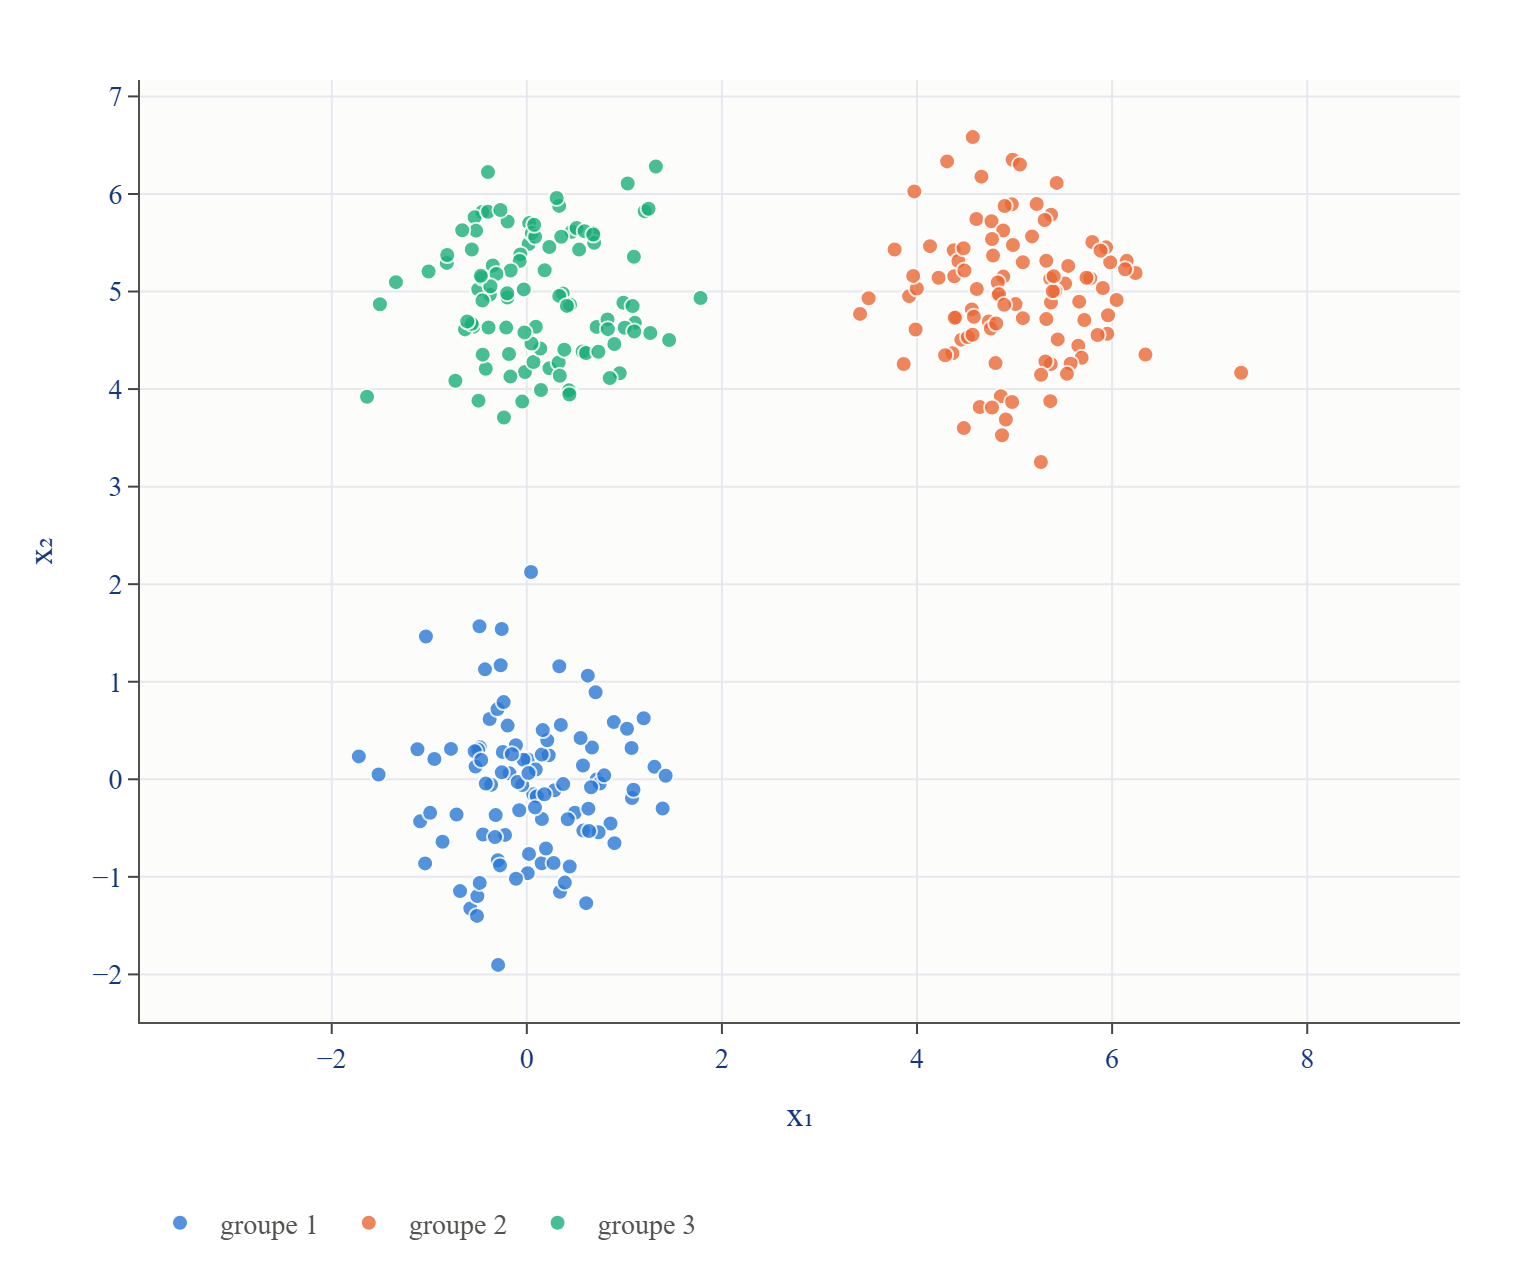
\includegraphics[width=0.85\textwidth]{figures/fig03.png}
\caption{Jeu de données synthétique utilisé pour l'étude expérimentale : trois groupes gaussiens réels de 100 observations chacun (N = 300 au total).}
\label{fig:2_2}
\end{figure}
\subsection{Scénarios synthétiques S1 à S10}\label{sec:scenarios_plan}
Les scénarios remplacent l'expérience unique du jeu de référence par des plans répliqués, chacun isolant un facteur que la thèse désigne comme décisif. Chaque point d'un plan est répété $R$ fois, $R$ étant fixé par le calcul de puissance (section~\ref{sec:calibrage}) ; données d'apprentissage et de test sont tirées avec des graines dérivées du rôle de chaque tirage. Le tableau~\ref{tab:scenarios_plan} résume les plans.

\begin{table}[H]
\centering
\small
\setlength{\tabcolsep}{0.1cm}
\begin{tabular}{|p{1.0cm}|p{3.0cm}|p{6.2cm}|p{4.6cm}|}
\hline
\textbf{Scén.} & \textbf{Facteur} & \textbf{Génération} & \textbf{Mesure principale} \\
\hline
S1 & Chevauchement & 3 gaussiennes de variance unité aux sommets d'un triangle, séparation de 1 à 5 écarts-types, $N=300$ & ARI, VB-emp contre EM-BIC \\
\hline
S2 & Poids déséquilibrés & Poids 80, 15 et 5 \%, séparation de 5 écarts-types & Perte de la composante minoritaire \\
\hline
S3 & Sous-estimation de $K$ & $K$ vrai de 4 à 6 (centres alignés, écart 4), $K$ choisi égal à 3 & ARI, VB à $K_{\max}=3$ contre EM à $K=3$ \\
\hline
S4 & Queues épaisses & Composantes de Student à 3 degrés de liberté & ARI \\
\hline
S5 & Dimension & $D \in \{2, 5, 10, 20\}$, séparation de 6 écarts-types & ARI \\
\hline
S6 & Petit effectif & $N \in \{30, 60, 120, 300, 1\,000\}$, test de 1\,000 points & Ajustements dégénérés, VB contre EM-$K_{\max}$ \\
\hline
S7 & Aberrations & Proportion de 1, 5 ou 10 \% de points uniformes, amplitude de 5, 10 ou 20 & ARI hors aberrations \\
\hline
S8 & Seuil $d/2$ de $\alpha_0$ & $\alpha_0 \in \{1;\,1{,}5;\,2;\,2{,}5;\,3;\,5;\,10\}$, covariances pleine, diagonale et sphérique & Composantes actives (descriptif) \\
\hline
S9 & Plan factoriel des priors & $\alpha_0$ (4 niveaux) $\times$ $\beta_0$ (3) $\times$ $\nu_0 - D$ (2) $\times$ échelle de $W_0$ (3) & Part de variance de $\hat K$ (descriptif) \\
\hline
S10 & Seuil d'activité & $\alpha_0 \in \{1/6;\,1;\,2{,}5;\,10\}$, seuils $N_k \geq 1$, 0,5, 1 et 5 \% de $N$ & Composantes actives (descriptif) \\
\hline
\end{tabular}
\caption{Plans des scénarios synthétiques}
\label{tab:scenarios_plan}
\end{table}

Le seuil théorique de S8 provient de Rousseau et Mengersen~\cite{rousseau2011} : $d/2 = 2{,}5$ (pleine), $2$ (diagonale) et $1{,}5$ (sphérique) en dimension 2. Cette théorie porte sur le posterior exact : un basculement observé ailleurs est une propriété du champ moyen, non une réfutation. Pour les covariances non pleines, le critère d'arrêt est une approximation (section~\ref{sec:impl_vb}).

\subsection{Iris}\label{sec:iris_methodo}
Le jeu Iris de Fisher~\cite{fisher1936} compte $N=150$ fleurs de trois espèces décrites par $D=4$ mesures en centimètres, non standardisées (fichier versionné). Il sert de première confrontation à des données réelles dont les groupes se chevauchent (versicolor et virginica) ; ses étiquettes, connues indépendamment des mesures, permettent de calculer l'ARI. La régularisation $\varepsilon I$ (section~\ref{sec:impl_em}) est une valeur absolue unique, calibrée sur l'ensemble des jeux, où les jeux synthétiques sont les plus nombreux ; en centimètres, elle peut dépasser certaines variances d'Iris (variance intra-espèce de la largeur des pétales : 0,0115~cm² pour setosa, 0,039 pour versicolor, 0,075 pour virginica, calculée sur le fichier). Les ajustements EM et MAP-EM sur Iris peuvent en être lissés.

\subsection{Prix alimentaires des marchés du Cameroun (cas pratique)}\label{sec:prix_methodo}
\textbf{Problème réel. }Le Cadre Harmonisé d'octobre 2025 estime que plus de 2,8 millions de personnes, soit 10 \% de la population analysée, seront en insécurité alimentaire aiguë (phase 3 ou plus) au Cameroun entre juin et août 2026, principalement dans l'Extrême-Nord, le Nord-Ouest et le Sud-Ouest~\cite{giews2026,fewsnet2026}. Les prix des denrées de base y connaissent des chocs brusques et de sens opposés : le prix moyen du maïs blanc a augmenté de 24 \% en un mois dans l'Extrême-Nord en août 2023~\cite{pam2023bulletin}, alors qu'en avril 2026 le maïs et le sorgho se vendaient à Kousseri, Mokolo et Mora de 40 à 50 \% moins cher qu'un an plus tôt, la demande d'exportation vers le Nigeria ayant reculé avec l'interdiction camerounaise d'exporter des céréales~\cite{fewsnet2026}. Le Programme alimentaire mondial (PAM) les classe chaque mois en phases d'alerte selon des seuils fixés à l'avance (indicateur ALPS, section~\ref{sec:ea_prix}). La question pratique est la suivante : \emph{un mélange gaussien peut-il apprendre des régimes de prix à partir des données, sans seuils fixés à l'avance, et attacher à chaque marché et à chaque mois une probabilité d'être en régime de tension, avec une incertitude sur cette probabilité ?}

\textbf{Lien avec la thèse. }Ce cas met à l'épreuve, sur un problème réel, la sélection de $K$ (nombre de régimes inconnu), le petit effectif (séries courtes et trouées, domaine où les priors pèsent le plus, comme en S6), la sensibilité aux hyperparamètres (HP5), l'incertitude de la probabilité d'alerte et sa couverture (HP6), et les queues épaisses (S4, S7). Les tests correspondants (HP1 à HP7, HPP1 à HPP6) figurent au tableau~\ref{tab:plan_tests} ; chacun peut conclure dans un sens ou dans l'autre, et l'équivalence est une issue légitime.

\textbf{Données. }Base de prix du PAM pour le Cameroun, diffusée sur la plateforme HDX~\cite{pam2026donnees} sous licence CC BY-IGO (redistribution autorisée avec attribution) : 77\,268 relevés de janvier 2005 à août 2026, 83 marchés. L'extrait utilisé (\texttt{data/prix/wfp\_cmr\_panier.csv}, versionné avec le code, empreinte SHA-256 vérifiée au chargement ; script \texttt{scripts/telecharger\_prix\_wfp.py}) retient les prix de détail en francs CFA par kilogramme de trois denrées de base : le \emph{maïs blanc} (céréale locale), le \emph{riz importé} (céréale importée, sensible au change et aux coûts d'importation) et le \emph{niébé} (légumineuse, source de protéines). Ce panier a été choisi d'après la seule couverture des séries, avant tout ajustement.

\textbf{Variables. }Pour la denrée $j$, le marché $m$ et le mois $t$, la variable est l'écart du log-prix à son niveau des douze mois précédents :
\[
e_j(m,t) = \ln p_j(m,t) - \frac{1}{|U|}\sum_{u \in U} \ln p_j(m,u), \qquad U = \{u \in [t-12,\, t-1] : p_j(m,u) \text{ relevé}\},
\]
définie si au moins trois relevés existent dans la fenêtre. Un écart de $+0{,}30$ correspond à un prix environ 35 \% au-dessus de son niveau récent. Cette variable est \emph{causale} (aucune information postérieure à $t$), insensible aux mois manquants, et elle retire la dérive lente des prix (inflation) ainsi que la saisonnalité moyenne sur une année. Une observation $(m,t)$ est retenue si les trois écarts sont définis : $x_{m,t} = (e_1, e_2, e_3) \in \mathbb{R}^3$. Les variables sont standardisées par la moyenne et l'écart-type de la seule période d'apprentissage.

\textbf{Nettoyage déclaré. }Un relevé est écarté s'il diffère d'un facteur au moins 3, dans le même sens, du relevé du mois précédent \emph{et} de celui du mois suivant : c'est un pic isolé d'un mois, aller-retour, typique d'une virgule décalée (par exemple 97, puis 995, puis 97 XAF/kg pour le maïs à Doukoula en août, septembre et octobre 2023). Un triplement suivi d'un retour en un mois n'est pas plausible pour une denrée de base au détail : la plus forte hausse mensuelle citée par les bulletins du PAM pour le maïs de l'Extrême-Nord est de 24 \%. La règle est fixée avant tout ajustement ; 21 relevés sont écartés, dont 14 en septembre 2023, et leur liste complète est archivée dans le dépôt du mémoire (annexe A, fichier \texttt{prix\_releves\_ecartes.csv}). Parce qu'elle utilise le relevé du mois suivant, cette règle convient à une analyse rétrospective mais pas, telle quelle, à une alerte en temps réel.

\textbf{Validation temporelle. }Apprentissage d'avril 2021 à décembre 2023 (562 observations, 50 marchés, 6 régions), test de janvier 2024 à août 2026 (493 observations, 27 marchés, 3 régions). La date de coupure a été choisie d'après le seul nombre d'observations, avant toute estimation, pour que l'évaluation porte sur des mois postérieurs à tout l'apprentissage~\cite{roberts2017}. La description des deux périodes est au tableau~\ref{tab:prix_descriptif} et la carte des marchés à la figure~\ref{fig:prix_marches}.

\tableauGenere{prix_descriptif}

\begin{figure}[H]
\centering
\IfFileExists{figures/prix_marches.png}{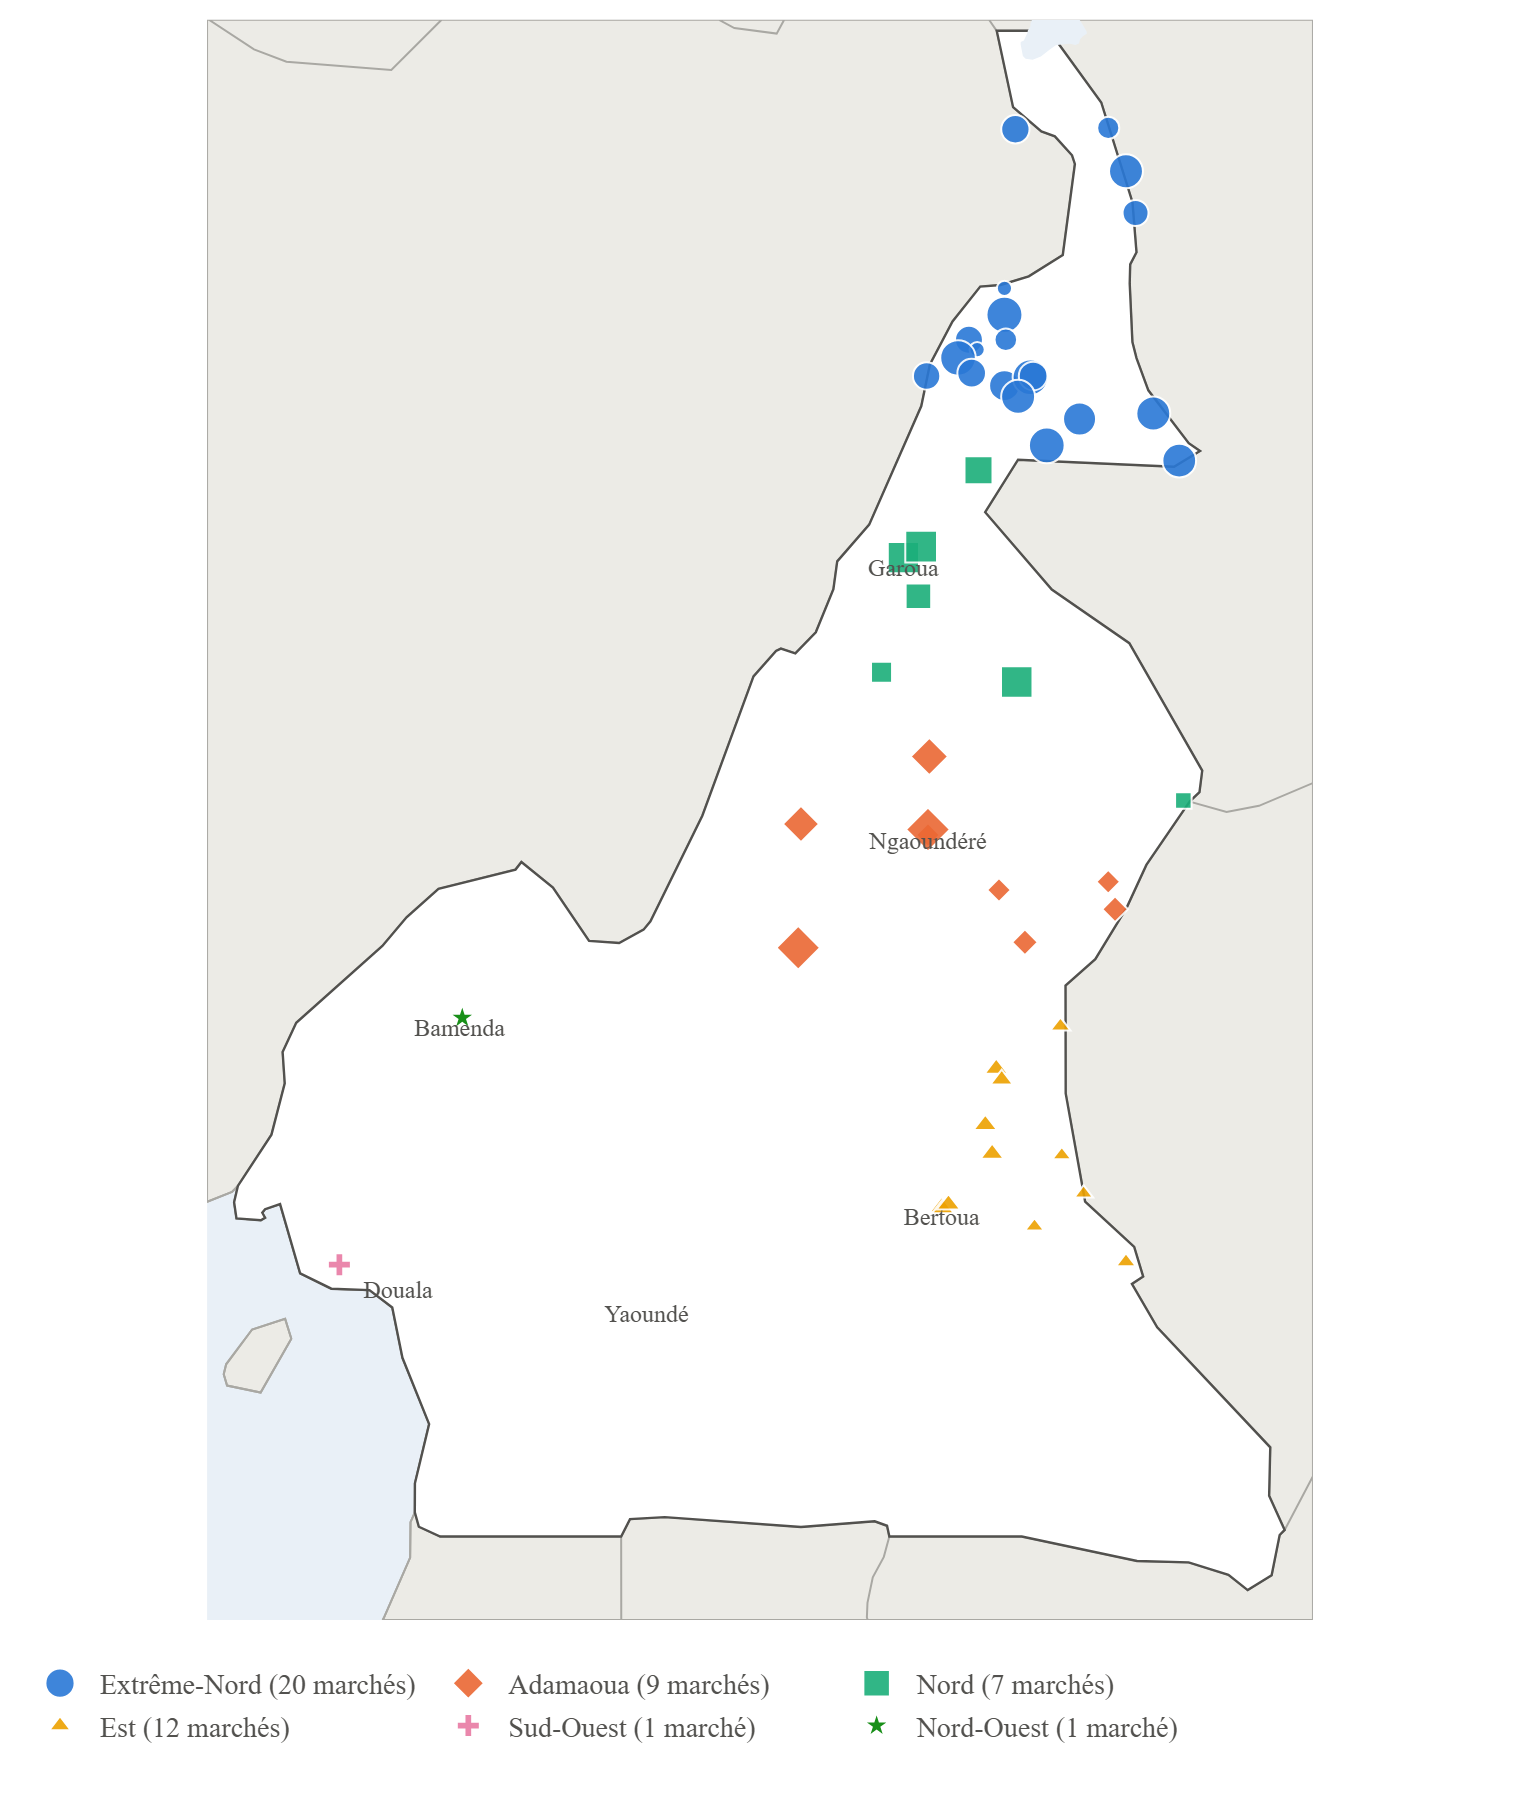
\includegraphics[width=0.62\textwidth]{figures/prix_marches.png}}{\fbox{\parbox{0.6\textwidth}{\centering figure à générer (\texttt{python run.py --figures})}}}
\caption{Marchés suivis : couleur et symbole par région (nombre de marchés entre parenthèses), taille selon le nombre d'observations retenues (apprentissage et test) ; quelques villes servent de repère. Sources : PAM, base de prix du Cameroun (HDX, CC BY-IGO) ; frontières Natural Earth.}
\label{fig:prix_marches}
\end{figure}

\textbf{Bras. }Les bras du chapitre~\ref{chap:methodologie}, avec le même critère d'arrêt (figure~\ref{fig:boucle_arret}), le même nombre de relances (registre, famille « prix ») et la covariance pleine : EM-$K_{\text{réf}}$, EM-$K_{\max}$, EM-BIC et EM-ICL ($K$ de 1 à $K_{\max}=8$), MAP-EM (priors empiriques et calibrés), VB à priors empiriques (VB-emp) et calibrés (VB-cal). $K_{\max}=8$ est le double des quatre phases usuelles d'alerte. Le \emph{régime de tension} d'un ajustement est la composante active dont la moyenne des trois écarts, en unités d'origine, est la plus élevée ; la \emph{probabilité d'alerte} d'une observation est sa responsabilité pour cette composante. Une observation est dite \emph{en alerte} lorsque cette probabilité dépasse 0,5. C'est la règle de décision de Bayes quand une fausse alerte et une alerte manquée ont le même coût : le seuil qui minimise le coût attendu vaut $c_{\text{FA}}/(c_{\text{FA}} + c_{\text{AM}})$, où $c_{\text{FA}}$ est le coût d'une fausse alerte et $c_{\text{AM}}$ celui d'une alerte manquée. Ces coûts relèvent des organismes de sécurité alimentaire et ne sont pas fixés ici.

\textbf{Plan. }(a) \emph{Référence} : EM-BIC sur toute la période d'apprentissage ; il fixe $K_{\text{réf}}$ et le modèle générateur du jeu semi-synthétique (tableau~\ref{tab:prix_reference}). (b) \emph{Sous-échantillons réels} : $N \in \{30, 60, 120, 250\}$ observations tirées dans l'apprentissage, tous les bras, évaluation sur toute la période de test. (c) \emph{Semi-synthétique} : jeux de taille $N \in \{30, 60, 120, 250, 500\}$ tirés du modèle de référence, de sorte que $K$, la partition et les paramètres vrais sont connus et réalistes. (d) \emph{Couverture} des intervalles à 90 \% sur le semi-synthétique ($N \geq 120$) : intervalles de crédibilité du VB (tirages de la loi variationnelle) et bootstrap non paramétrique de l'EM à démarrage chaud, appariés aux composantes vraies par l'algorithme hongrois ; une composante vraie sans composante active appariée compte comme non couverte (couverture inconditionnelle), une indicatrice est tirée par paramètre scalaire et l'intervalle de la couverture est un bootstrap \emph{par grappes} de réplications. (e) \emph{Sensibilité} : $\hat K$ du VB sur les configurations de priors plausibles issues du calibrage, contre $\hat K$ de EM-BIC entre graines. (f) \emph{Prévision} : log-score de chaque observation de test pour chaque modèle ajusté sur tout l'apprentissage. (g) \emph{Alerte} : probabilité de tension de chaque observation, avec son intervalle à 90 \%. Les nombres de réplications sont fixés par le calcul de puissance (registre, clés \texttt{prix\_sous}, \texttt{prix\_semi}, \texttt{prix\_sensibilite}).



Les observations d'un même mois partagent les chocs communs (prix internationaux, change, saison) : pour les comparaisons de prévision, la différence de log-score est d'abord moyennée par mois, puis le test de Diebold et Mariano~\cite{diebold1995} porte sur la série mensuelle. Le nombre de réplications écartées d'une comparaison appariée (bras en échec numérique) est rapporté dans la colonne « Exclues » des tableaux de décision.

\subsection{Corpus de texte (pLSA contre LDA)}\label{sec:texte_methodo}
\textbf{Niveaux d'inférence. }La LDA de Blei, Ng et Jordan~\cite{blei2003} est présentée à tort comme un exact analogue du GMM bayésien. Au sens de la figure~\ref{fig:trois_niveaux}, la LDA du code est un \emph{EM variationnel à $\beta$ ponctuel} : $q(\theta_d)$ est un Dirichlet (paramètres $\gamma_d$), mais les distributions de mots par thème $\beta_k$ sont des paramètres ponctuels estimés à l'étape M et $\alpha$ est fixé. Elle n'est pas un VB complet. Son étape E, un point fixe sur $(\phi_d, \gamma_d)$, s'arrête à la tolérance commune ou après au plus 100 itérations par étape M, valeur par défaut de scikit-learn~\cite{pedregosa2011} ; chaque itération augmente la borne, qui reste donc croissante, et le nombre d'étapes E plafonnées est rapporté. La correspondance avec le GMM est donc partielle : $\gamma_k \leftrightarrow \alpha_k$ vaut pour les poids de mélange ($\theta_d$ joue le rôle de $\pi$ par document), mais $\beta_k$ n'a pas de prior (contrairement à $(\mu_k,\Lambda_k)$ dans le GMM bayésien). Le comparateur « EM classique » de la LDA est le pLSA~\cite{hofmann1999}, qui estime $\theta_d$ et $\beta_k$ par maximum de vraisemblance sans prior.

Ce placement suit le texte original : Blei, Ng et Jordan~\cite[section~5.3]{blei2003} estiment $\alpha$ et $\beta$ ponctuellement par un EM variationnel de type Bayes empirique ; leur variante « lissée » (section 5.4), reprise par Hoffman et al.~\cite{hoffman2013} avec la SVI, place un prior de Dirichlet sur chaque $\beta_k$ et relève du niveau 3. La LDA du code correspond à la version non lissée, à $\alpha$ fixé : la comparaison pLSA contre LDA mesure l'effet du prior sur $\theta_d$ seul, non celui d'un traitement bayésien complet.

\begin{figure}[H]
\centering
\begin{tikzpicture}[>=Stealth,
    v/.style={circle,draw=navy,minimum size=0.9cm,font=\footnotesize,inner sep=0pt},
    o/.style={circle,draw=navy,fill=ciel!40,minimum size=0.9cm,font=\footnotesize,inner sep=0pt}]
  \node[font=\footnotesize\bfseries] at (1.7,3.0) {pLSA (EM, sans prior)};
  \node[v] (theta1) at (0,1.8) {$\theta_d$};
  \node[v] (z1) at (1.8,1.8) {$z$};
  \node[o] (w1) at (3.4,1.8) {$w$};
  \node[font=\scriptsize] (phi1) at (3.4,0.4) {$\phi_k$ ponctuel};
  \draw[->] (theta1) -- (z1);
  \draw[->] (z1) -- (w1);
  \draw[->] (phi1) -- (w1);
  \node[font=\scriptsize,text=gray] at (0,0.9) {ponctuel, sans prior};
  \node[font=\footnotesize\bfseries] at (9.4,3.0) {LDA (EM variationnel)};
  \node[font=\scriptsize] (alpha) at (6.4,1.8) {$\alpha$};
  \node[v] (theta2) at (7.8,1.8) {$\theta_d$};
  \node[v] (z2) at (9.4,1.8) {$z$};
  \node[o] (w2) at (11,1.8) {$w$};
  \node[font=\scriptsize] (beta2) at (11,0.4) {$\beta_k$ ponctuel};
  \draw[->] (alpha) -- (theta2);
  \draw[->] (theta2) -- (z2);
  \draw[->] (z2) -- (w2);
  \draw[->] (beta2) -- (w2);
  \node[font=\scriptsize,text=gray] at (7.8,0.9) {$\sim\mathrm{Dir}(\alpha)$, prior};
\end{tikzpicture}
\caption{Modèles graphiques du pLSA et de la LDA utilisée ici. La différence testée est le prior de Dirichlet sur $\theta_d$ (LDA) contre un $\theta_d$ ponctuel sans prior (pLSA). Dans les deux cas les distributions de mots par thème sont ponctuelles : la LDA du code est un EM variationnel à $\beta$ ponctuel, non un VB complet.}
\label{fig:plsa_lda}
\end{figure}


\textbf{Hypothèse (HT1, rattachée à RH4). }Le pLSA sur-apprend davantage que la LDA quand le nombre de documents $N$ est petit (le prior de Dirichlet sur $\theta_d$ est la raison d'être de la LDA) ; l'écart se réduit quand $N$ croît. Elle est testée par la différence appariée, par $N \in \{50, 200, 1\,000\}$, de l'écart relatif entre perplexité hors échantillon et perplexité sur les documents d'apprentissage.

\textbf{Données et protocole. }Sous-ensemble de 20 Newsgroups (quatre groupes : \texttt{sci.space}, \texttt{rec.sport.baseball}, \texttt{talk.politics.mideast}, \texttt{comp.graphics}), lu directement dans l'archive originale \texttt{20news-bydate.tar.gz}, sans bibliothèque d'apprentissage ; jeu de diffusion libre pour la recherche, sans licence explicite (à citer :~\cite{lang1995}). Prétraitement, fixé avant l'analyse et identique pour les deux modèles : suppression des en-têtes, des lignes de citation et des signatures ; minuscules ; seules les suites de lettres sont gardées (ponctuation et chiffres écartés) ; mots d'au moins trois lettres, racinisés par l'algorithme de Porter~\cite{porter1980} écrit pour ce travail ; vocabulaire des 1\,500 racines les plus fréquentes parmi celles présentes dans au moins cinq documents et dans au plus la moitié d'entre eux. Les mots vides sont écartés par ce seul critère de fréquence documentaire, sans liste externe ; les documents comptant moins de vingt occurrences de mots du vocabulaire sont exclus. La sensibilité des conclusions à la taille du vocabulaire (500 et 3\,000 racines) est mesurée. La perplexité hors échantillon est calculée par complétion de document (la moitié des mots d'un document sert à estimer $\theta_d$, l'autre à l'évaluer, de façon identique pour les deux modèles) ; la cohérence des thèmes est mesurée par le NPMI des dix premiers mots ; la pureté est calculée par rapport aux étiquettes du corpus. Les deux modèles partagent le critère d'arrêt de la figure~\ref{fig:boucle_arret}. Les probabilités sont planchées à $10^{-12}$ et la part de mots planchés est rapportée.

\section{Plan d'échantillonnage}\label{sec:echantillonnage}
\textbf{Taille de l'échantillon. }L'unité d'échantillonnage est la \emph{réplication} : un jeu de données tiré, sur lequel tous les bras sont ajustés. Le nombre de réplications de chaque famille de plans est fixé avant les calculs confirmatoires par un calcul de puissance (puissance d'au moins 0,8 au niveau de la première étape de Holm), à partir de réplications pilotes dont les graines sont disjointes de celles des étapes confirmatoires ; une hypothèse sans variance pilote ne fixe pas ce nombre, et celui-ci est plafonné par un budget de temps déclaré, la puissance obtenue étant rapportée (section~\ref{sec:calibrage}). Les tailles des tirages Monte Carlo (bootstrap, tirages a posteriori) sont fixées par une règle de précision des bornes rapportées.

\textbf{Méthode d'échantillonnage. }Les jeux synthétiques sont tirés par simulation selon le plan de chaque scénario. Pour les prix, des sous-échantillons de $N \in \{30, 60, 120, 250\}$ observations sont tirés aléatoirement, sans remise, dans la période d'apprentissage, et des jeux semi-synthétiques de $N \in \{30, 60, 120, 250, 500\}$ observations sont simulés à partir du modèle de référence ; la comparaison de prévision utilise au contraire une séparation \emph{temporelle} (apprentissage d'avril 2021 à décembre 2023, test de janvier 2024 à août 2026), afin de ne pas évaluer un modèle sur des mois antérieurs à ses données. Pour le texte, des échantillons de $N \in \{50, 200, 1000\}$ documents sont tirés dans le réservoir d'apprentissage. Chaque tirage reçoit une graine dérivée de son rôle (annexe D).

\textbf{Justification. }Le tirage aléatoire simple et la simulation donnent des réplications indépendantes, condition des tests appariés de la section~\ref{sec:decision} ; les tailles croissantes isolent l'effet de l'effectif, central pour l'hypothèse RH4 ; la séparation temporelle reproduit l'usage réel d'un modèle d'alerte.

\section{Méthodes d'analyse : protocole de comparaison}\label{sec:protocole}
\subsection{Bras comparés et critère d'arrêt commun}\label{sec:bras_compares_et_critere_d}
Tous les bras sont ajustés sur les mêmes données, avec le même critère d'arrêt, le même nombre de relances et la même graine d'ajustement : EM-$K$ ($K$ de référence), EM-$K_{\max}$ (même capacité que le VB), EM-BIC et EM-ICL ($K$ choisi par balayage de 1 à $K_{\max}$), MAP-EM (priors Normal-Wishart du VB, Dirichlet plat $\alpha_0 = 1$, sans loi sur les paramètres), VB à priors empiriques (VB-emp), diffus (VB-diff) et calibrés (VB-cal). Une composante est active si $N_k/N$ dépasse le seuil du registre, et $\hat K$ est le nombre de composantes actives, avec la même règle pour tous les bras. Le schéma de la figure~\ref{fig:protocole} résume le protocole et celui de la figure~\ref{fig:boucle_arret} le critère d'arrêt commun.

\begin{figure}[H]
\centering
\begin{tikzpicture}[>=Stealth,
    b/.style={draw=navy,rounded corners=2pt,align=center,font=\scriptsize,fill=ciel!20,minimum height=0.8cm,text width=2.5cm},
    g/.style={draw=bleu,rounded corners=2pt,align=center,font=\scriptsize,fill=bleu!15,minimum height=0.55cm,text width=3.4cm}]
  \node[b] (don) at (0,0) {données (au moins 30 réplications, graines fixées)};
  \node[g] (a1) at (4.2,1.95) {EM-$K$ ($K$ connu)};
  \node[g] (a2) at (4.2,1.3)  {EM-$K_{\max}$};
  \node[g] (a3) at (4.2,0.65) {EM-BIC};
  \node[g] (a4) at (4.2,0)    {EM-ICL};
  \node[g] (a5) at (4.2,-0.65) {MAP-EM};
  \node[g] (a6) at (4.2,-1.3) {VB, priors empiriques};
  \node[g] (a7) at (4.2,-1.95) {VB, priors diffus};
  \node[b] (mes) at (7.9,0) {mesures : $\hat K$, ARI, log-vraisemblance hors échantillon, dégénérescence, temps};
  \node[b] (tst) at (11.5,0) {tests appariés, TOST, Wilcoxon, correction de Holm};
  \draw[->] (don) -- (a1.west);
  \draw[->] (don) -- (a4.west);
  \draw[->] (don) -- (a7.west);
  \draw[->] (a1.east) -- (mes.west);
  \draw[->] (a4.east) -- (mes.west);
  \draw[->] (a7.east) -- (mes.west);
  \draw[->] (mes) -- (tst);
  \node[font=\scriptsize,text=navy] at (5.9,-2.7) {même critère d'arrêt (figure~\ref{fig:boucle_arret}) pour tous les bras};
\end{tikzpicture}
\caption{Protocole « 5 EM + VB » : tous les bras partagent le critère d'arrêt, les graines et les mesures ; chaque comparaison est appariée par réplication.}
\label{fig:protocole}
\end{figure}

\begin{figure}[H]
\centering
\begin{tikzpicture}[>=Stealth,
    boite/.style={draw=navy,rounded corners=2pt,minimum height=0.9cm,align=center,font=\footnotesize,fill=ciel!20,text width=3.0cm},
    test/.style={draw=bleu,rounded corners=2pt,align=center,font=\footnotesize,fill=bleu!12,text width=3.6cm,minimum height=1.1cm}]
  \node[boite] (init) at (0,0) {initialisation\\$\theta_0$ ou $q_0$, $n_M=0$};
  \node[boite] (E) at (4.2,0) {étape E\\$r_{ik}$ et critère $c_t$};
  \node[test] (T) at (8.8,0) {$\lvert c_t-c_{t-1}\rvert\le \mathrm{tol}\cdot\max(\lvert c_{t-1}\rvert,1)$ ?};
  \node[boite,fill=navy!15] (S) at (13.0,0) {arrêt\\\texttt{converge}=vrai};
  \node[test] (P) at (8.8,-2.2) {$n_M=500$ ?\\sinon étape M};
  \node[boite,fill=navy!15] (S2) at (13.0,-2.2) {arrêt\\\texttt{converge}=faux};
  \node[boite] (M) at (4.2,-2.2) {étape M\\$n_M\leftarrow n_M+1$};
  \draw[->] (init) -- (E);
  \draw[->] (E) -- (T);
  \draw[->] (T) -- node[above,font=\scriptsize]{oui} (S);
  \draw[->] (T) -- node[right,font=\scriptsize]{non} (P);
  \draw[->] (P) -- node[above,font=\scriptsize]{oui} (S2);
  \draw[->] (P) -- node[above,font=\scriptsize]{non} (M);
  \draw[->] (M) -- (E);
\end{tikzpicture}
\caption{Critère d'arrêt commun à l'EM, au MAP-EM, à l'EM variationnel et au pLSA. Le critère $c$ est la log-vraisemblance totale (EM) ou l'ELBO total (VB, covariance pleine), évalué après chaque étape E et avant l'étape M. Tolérance relative $10^{-6}$ et plafond commun de 500 étapes M ; $n_M$ est le nombre d'itérations rapporté.}
\label{fig:boucle_arret}
\end{figure}

\subsection{Métriques}\label{sec:metriques}
L'ARI suppose une vérité terrain et dépend du nombre de composantes ; la silhouette n'est comparable qu'à $K$ égal et n'est pas utilisée comme preuve. Les plans rapportent donc aussi la log-vraisemblance moyenne hors échantillon (plug-in pour tous les bras ; loi prédictive de Student en plus pour le VB, afin de séparer l'effet de la loi prédictive de celui des priors), l'erreur $\lvert \hat K - K \rvert$ lorsque $K$ est connu, et la fréquence d'ajustements dégénérés (valeur propre minimale de $\Sigma_k$ inférieure à $10^{-6}$ fois sa trace, ou $N_k < D+1$). Pour le cas pratique s'ajoutent la probabilité d'alerte (responsabilité du régime de tension), son intervalle à 90 \% (tirages de la loi variationnelle pour le VB, bootstrap à démarrage chaud pour l'EM) et le log-score de chaque observation de la période de test. Les temps sont mesurés dans un seul processus et un seul fil, en temps total jusqu'au modèle final.

\subsection{Tests statistiques et règle de décision}\label{sec:decision}
Chaque test déclaré porte sur les différences appariées $d_r = A_r - B_r$ des réplications $r$. Un test d'\emph{équivalence} est un TOST~\cite{schuirmann1987} à une marge fixée avant tout résultat confirmatoire : la plus petite différence d'intérêt, choisie par l'importance pratique~\cite{lakens2017,lakens2018}. Pour l'ARI, indice de référence de la validation des classifications~\cite{steinley2004}, la marge vaut 0,05, soit 5 \% de l'écart entre un accord dû au hasard (ARI nul) et un accord parfait (ARI égal à 1). Pour la log-vraisemblance moyenne par observation, elle vaut 0,05 nat, soit environ $\log 1{,}05$ : la densité prédictive d'une méthode dépasse celle de l'autre d'au plus 5 \% en moyenne géométrique, le même seuil relatif que pour l'ARI. Les décisions sont aussi rapportées à la moitié et au double de chaque marge, et le bruit d'optimisation (écart entre deux ajustements d'une même méthode) est mesuré pour vérifier que chaque marge le dépasse ; un test de \emph{différence} est le test des rangs signés de Wilcoxon, calculé par sa loi exacte de permutation. La correction de Holm~\cite{holm1979} est appliquée au sein de chaque famille (scénarios, prix, prévision, texte), et la décision est prise sur la probabilité critique \emph{ajustée}. L'estimation rapportée est la moyenne des différences, avec son intervalle bootstrap percentile à 95 \%, ainsi que l'estimateur de Hodges et Lehmann~\cite{hodges1963}, médiane des moyennes de Walsh $(d_i + d_j)/2$ pour $i \leq j$ ; c'est cet estimateur, cohérent avec le test de Wilcoxon, qui donne le sens d'une différence significative (la moyenne quand il est nul, ce qui arrive pour des indicatrices dont la plupart des différences sont nulles). Les réplications où un bras échoue numériquement sont exclues de la comparaison et leur nombre est rapporté (colonne « Exclues »). Les comparaisons de prévision du cas pratique utilisent le test de Diebold et Mariano~\cite{diebold1995}, avec la correction de Harvey, Leybourne et Newbold~\cite{harvey1997}, sur la série \emph{mensuelle} des différences de log-score : les observations d'un même mois partagent des chocs communs et ne sont pas indépendantes.

Le verdict d'une décision au regard de son hypothèse de recherche est déclaré ainsi : \emph{conforme} si la décision est celle qu'attend l'hypothèse ; \emph{contraire} si elle démontre l'effet opposé ; \emph{non tranché} si le test ne conclut pas (une équivalence non démontrée n'est pas une différence démontrée) ; une différence démontrée pour un test non orienté est rapportée sans être comptée pour ni contre l'hypothèse. Le bilan d'une hypothèse de recherche est le décompte de ces verdicts sur tous ses tests ; il n'est pas résumé par une seule probabilité.

\subsubsection*{Couverture des intervalles (HP6)}\label{sec:couverture}
La sous-estimation de variance du champ moyen (section~\ref{sec:kl_inverse}) ne peut être jugée que par la couverture empirique des intervalles à 90 \% sur des jeux dont les paramètres vrais sont connus. Elle constitue une \emph{prédiction théorique testée} : le champ moyen sous-estime la variance a posteriori~\cite[section~10.1.2]{bishop2006}, \cite{blei2017}, et les intervalles qui en découlent sont trop étroits dans les mélanges~\cite{wang2005}. La mesure est faite sur le jeu semi-synthétique du cas pratique (section \ref{sec:res_prix}, hypothèse HP6), pour le VB et pour le bootstrap de l'EM-BIC, qui choisit $K$ par le BIC sur chaque jeu simulé comme le VB choisit le sien ; la comparaison porte sur la différence de couverture entre les deux, appariée par réplication. Le bootstrap de l'EM au $K$ de référence, qui connaît $K$, sert de borne favorable à l'EM. Les deux bootstraps sont conditionnels au $K$ retenu : ils ne propagent pas l'incertitude du choix de $K$, de même que les intervalles du VB sont conditionnels à sa structure élaguée. La couverture est \emph{inconditionnelle} (une composante vraie sans composante active appariée compte comme non couverte) ; une indicatrice est tirée par paramètre scalaire, et l'intervalle de la couverture est un bootstrap par grappes de réplications, les indicatrices d'une même réplication n'étant pas indépendantes. Les intervalles de crédibilité et de confiance ne mesurent pas le même objet : leur couverture sur la valeur vraie est une comparaison de calibration, non de justesse bayésienne.

\section{Calibrage des paramètres}\label{sec:calibrage}
Aucune valeur méthodologique n'est choisie à la main. Chaque paramètre est inscrit dans un registre (\texttt{parametres.py} ; valeurs principales au tableau~\ref{tab:registre_resume}, annexe E) avec un statut : \emph{mathématique} (conséquence d'un résultat), \emph{source} (valeur prescrite par une référence vérifiée), \emph{plan} (choix de conception déclaré), ou \emph{calibré} par une étude écrite dans le code. Tant qu'une valeur calibrée manque, l'orchestrateur refuse les étapes confirmatoires. Le calibrage s'exécute en sept vagues, chacune n'utilisant que des valeurs fixées par les vagues précédentes, et uniquement des données d'apprentissage (jamais la période de test du cas pratique) :
\begin{enumerate}
\item plafond des itérations de Lloyd pour l'initialisation par k-means (au plus 1 \% des exécutions l'atteignent) ;
\item tolérance d'arrêt et plafond d'étapes M : plus grande tolérance dont 99 \% des ajustements s'accordent avec une référence à $10^{-10}$ sur le critère final (écart par observation inférieur à $5 \times 10^{-4}$), l'accord des partitions étant rapporté ; si aucune tolérance ne remplit la règle, le calibrage s'arrête ;
\item régularisation $\varepsilon$ des covariances : rang moyen de la log-vraisemblance hors pli (blocs temporels contigus pour les prix), sur une grille de 0 à 1, une valeur au bord de la grille étant signalée ;
\item nombre de relances : 20 pour toutes les familles et pour EM comme pour VB ; pour chaque cas pilote est rapportée la probabilité que la meilleure des 20 relances soit à moins de $5 \times 10^{-4}$ par observation de la meilleure de 200 relances pilotes~\cite{biernacki2003} ; pour l'étape texte, plus petit nombre de relances (au plus 20) dont la meilleure est, avec une probabilité d'au moins 0,99, à moins de 0,1~\% de la meilleure des 200 relances pilotes ;
\item hyperparamètres du bras VB-cal (recherche aléatoire puis divisions successives~\cite{bergstra2012,jamieson2016}), hyperparamètres de la LDA et pas des variantes stochastiques, par validation croisée ;
\item contrôle des marges d'équivalence, fixées a priori (le bruit d'optimisation entre deux graines doit rester inférieur à la marge), et tailles Monte Carlo (erreur des bornes inférieure à la moitié de la dernière décimale affichée) ;
\item nombre de réplications : plus petit $R$ donnant une puissance simulée d'au moins 0,8 au niveau de la première étape de Holm, d'après des réplications pilotes à graines disjointes ; une hypothèse sans variance pilote ne fixe pas $R$, et $R$ est plafonné par un budget de temps déclaré, la puissance obtenue étant rapportée pour chaque hypothèse.
\end{enumerate}
Chaque vague écrit sa valeur, sa règle et ses évaluations dans \texttt{resultats/calibrage/}, ce qui rend chaque choix traçable.

\section{Implémentation et ingénierie du code}\label{sec:implementation}
\subsection{EM classique}\label{sec:impl_em}
L'EM classique est implémenté en PyTorch~\cite{paszke2019} à partir des équations du chapitre~\ref{chap:fondements}, sans bibliothèque de modélisation : seules les opérations élémentaires (algèbre linéaire, factorisation de Cholesky, fonction digamma) sont utilisées, et les critères d'évaluation (BIC, AIC, indice de Rand ajusté, silhouette) sont écrits explicitement. Le code complet figure à l'annexe A ; les extraits ci-dessous montrent la correspondance avec les équations.

\subsubsection*{Étapes E et M}
La densité gaussienne est évaluée par la factorisation de Cholesky de la covariance (section~\ref{sec:comportement_numerique_et_stabilite}), puis l'étape E calcule les responsabilités en log-espace avec l'astuce du log-sum-exp (équations~\ref{eq:1_15} et \ref{eq:1_18}). L'étape M applique les mises à jour de l'équation~\eqref{eq:1_16}. Le code de ces étapes, dans sa version exécutée qui traite toutes les relances en un seul lot, est reproduit à l'annexe A, avec la correspondance entre fonctions, sections et équations.

\subsubsection*{Initialisation, relances et critère d'arrêt}\label{sec:impl_em_init}
Deux initialisations sont disponibles : par k-means (avec initialisation k-means++), qui donne un point de départ proche de la solution, et aléatoire (K points de données tirés au hasard et covariance globale, section~\ref{sec:formulation_mathematique_complete}.a). L'algorithme est relancé n\_init fois et la solution de plus grande log-vraisemblance est conservée. Le critère d'arrêt est celui de la figure~\ref{fig:boucle_arret}, commun à l'EM, au MAP-EM, au VB et au pLSA : variation relative du critère \emph{total} inférieure à la tolérance calibrée, plafond d'étapes M calibré, la sortie rapportant \texttt{converge} (faux si le plafond est atteint : l'exécution est alors « non convergée »). Chaque covariance reçoit $+\,\varepsilon I$, $\varepsilon$ étant calibré par validation croisée (registre, \texttt{reg\_covariance}) : l'EM utilisé dans ce mémoire est donc régularisé, ce qui en fait un maximum local de la vraisemblance régularisée (section~\ref{sec:proprietes_em}.a). Le code retourne aussi l'ICL, l'entropie des affectations et un indicateur de dégénérescence.

\subsection{EM variationnel}\label{sec:impl_vb}
L'EM variationnel pour le GMM bayésien est implémenté de la même façon. Les espérances nécessaires (équations~\ref{eq:1_29} et \ref{eq:1_30}) sont calculées avec la fonction digamma de PyTorch, les mises à jour suivent les équations~\eqref{eq:1_26} et \eqref{eq:1_28}, et l'ELBO de l'équation~\eqref{eq:1_31} est évaluée exactement à chaque itération (annexe B). L'étape E variationnelle est reproduite à l'annexe A.

\subsubsection*{Étapes E et M variationnelles}
Les variantes de covariance tied, diag et spherical, absentes du chapitre~\ref{chap:fondements}, sont obtenues avec un prior de Wishart partagé ou des priors Gamma sur les précisions. Leur ELBO n'est ni dérivée ni implémentée : le critère d'arrêt est la somme des log-normalisations de l'étape E, c'est-à-dire l'ELBO privée du terme $\mathrm{KL}[q(\theta)\Vert p(\theta)]$, qui n'est pas nécessairement monotone. Ces variantes sont donc une \emph{approximation} (clé \texttt{critere\_nom} = \texttt{approximation\_log\_norm}) et les conclusions qui les concernent sont formulées en conséquence ; le terme $D/\beta_k$ de l'étape E reste exact pour ces priors.

\subsection{Orchestration reprenable et production des résultats}\label{sec:architecture}
Les expériences sont organisées en étapes (calibrage, validation, illustrations, chronométrage, scénarios, prix, texte), chacune étant une liste d'unités indépendantes exécutées en parallèle. Chaque unité terminée est écrite de façon atomique dans un magasin d'artefacts ; les longs ajustements sauvegardent périodiquement l'état complet de leur boucle. Un calcul interrompu (erreur, coupure de courant, arrêt volontaire) reprend donc exactement où il s'était arrêté, sans rien recalculer, et un superviseur relance automatiquement le calcul après un arrêt non voulu. Les tableaux et les figures du chapitre~\ref{chap:resultats} sont produits depuis ce magasin, sans recalcul ; les lectures factuelles qui accompagnent les décisions sont, elles aussi, écrites par le code à partir des fichiers de résultats. Aucun nombre des résultats n'est saisi à la main.

\section{Considérations éthiques}\label{sec:ethique}
Le travail n'implique aucune enquête auprès de personnes et ne requiert donc pas de consentement éclairé. Toutes les données sont secondaires et publiques. Les prix du PAM sont diffusés sous licence CC BY-IGO, qui autorise la réutilisation avec attribution~\cite{pam2026donnees} ; ils portent sur des marchés, non sur des personnes. Le corpus 20 Newsgroups est diffusé librement pour la recherche~\cite{lang1995} ; les en-têtes (adresses et noms des expéditeurs) et les signatures sont retirés au prétraitement, et seuls des comptes de mots sont conservés. Iris est un jeu public~\cite{fisher1936}. Aucune donnée personnelle n'est donc traitée ni publiée. Les résultats sur les prix décrivent des régimes statistiques et ne constituent pas un dispositif d'alerte opérationnel : ils ne doivent pas être utilisés pour des décisions d'assistance sans validation par les organismes compétents. Le code et l'extrait de données utilisé sont publiés (annexe A) ; chaque tableau et chaque figure peuvent être régénérés par le code, ce qui permet de vérifier chaque chiffre.

\section{Limites de la méthodologie : menaces à la validité et écarts au protocole}\label{sec:validite}
\textbf{Validité interne. }Les comparaisons utilisent le même critère d'arrêt, les mêmes relances et les mêmes graines pour tous les bras ; l'EM du code est régularisé par $\varepsilon I$, avec la valeur calibrée $\varepsilon = 0{,}1$ (section~\ref{sec:calibrage}), de sorte qu'aucune comparaison n'oppose un « EM non protégé » à un « VB protégé ». Les priors empiriques réutilisent les données (Bayes empirique) : le bras VB-diff et le plan factoriel S9 en mesurent l'effet. Le jeu semi-synthétique du cas pratique est tiré du modèle EM-BIC de référence, et l'erreur sur $K$ (HP1) est mesurée par rapport au $K_{\text{réf}}$ que ce bras a choisi : la vérité est fabriquée par l'un des bras comparés, ce qui peut avantager EM-BIC par construction. Ce n'est pas une fuite d'information (les jeux simulés sont indépendants des données d'ajustement), mais les résultats semi-synthétiques se lisent sous cette réserve.

\textbf{Validité externe. }Les scénarios reposent sur des mélanges gaussiens (ou de Student) simples, de dimension au plus 20. Le cas pratique porte sur trois denrées, des séries courtes et trouées, et une période de test qui ne couvre que trois régions et dont la distribution diffère de l'apprentissage ; ses conclusions ne s'étendent pas d'elles-mêmes aux autres régions ou pays.

\textbf{Validité de construit. }L'ARI suppose une vérité terrain ; le nombre de composantes actives dépend du seuil d'activité (S10) ; un « régime de tension » est une composante du mélange, non un état observé. Les mesures sans étiquette (log-vraisemblance et log-score hors échantillon) complètent donc l'ARI.

\textbf{Validité statistique. }Les observations spatiales et temporelles réelles ne sont pas indépendantes : la validation temporelle et l'agrégation mensuelle des comparaisons de prévision atténuent ce problème sans le supprimer. Les tests sont corrigés par famille, la puissance est fixée a priori, et les exclusions dues aux échecs numériques sont rapportées.

\textbf{Écarts au protocole.} (1) Les tests des scénarios ont été formalisés, un seul par hypothèse, après une première exécution exploratoire. (2) Les tests du cas pratique ont été déclarés le 27 octobre 2026, après la seule description de la couverture des données et avant tout ajustement de modèle ; le même jour, après un essai technique de la chaîne (deux réplications, paramètres provisoires, résultats non utilisés), le rattachement aux hypothèses de recherche a été ajouté, la sensibilité aux priors (HP5) est passée d'un constat descriptif à un test apparié, et le test HP7 a été ajouté pour isoler l'effet des priors. (3) La règle de nettoyage des relevés de prix a été fixée après l'inspection des données brutes, avant tout ajustement. (4) La réplication du jeu de référence sur trente tirages des versions antérieures est remplacée par les scénarios répliqués S1 à S10. (5) Le 4 novembre 2026, avant tout résultat confirmatoire, cinq règles ont été modifiées. Les marges d'équivalence, d'abord tirées du bruit d'optimisation (écart entre deux ajustements d'une même méthode), sont désormais fixées a priori par l'importance pratique : 0,05 pour l'ARI et 0,05 nat par observation pour la log-vraisemblance (section~\ref{sec:calibrage}) ; la règle antérieure rendait l'équivalence presque impossible à démontrer, quelles que soient les méthodes, et le bruit d'optimisation sert désormais de contrôle. Une hypothèse dont les différences pilotes sont toutes identiques ne fixe plus le nombre de réplications de sa famille, et ce nombre est plafonné par un budget de temps, la puissance obtenue étant rapportée pour chaque hypothèse. La dégénérescence est comptée avec le même critère pour tous les bras (petite composante, ou valeur propre minimale inférieure à $10^{-6}$ fois la trace de la covariance finale), alors que le critère antérieur ne pouvait signaler un effondrement que pour l'EM. La couverture (HP6) compare le VB au bootstrap d'EM-BIC, qui choisit $K$ comme le VB, le bootstrap à $K$ connu servant de borne. Le sens d'une différence significative est donné par l'estimateur de Hodges-Lehmann, cohérent avec le test de Wilcoxon, et non plus par le signe de la moyenne. (6) Le 5 novembre 2026, avant tout résultat confirmatoire du texte, le nombre de relances des ajustements pLSA et LDA de l'étape texte et de ses pilotes a été séparé de celui du calibrage. La règle commune exigeait de retrouver la même solution ; pour le pLSA, dont les optima de qualité voisine sont nombreux, elle imposait le plafond de 200 relances et un coût hors budget. La règle retenue est le plus petit nombre de relances, au plus 20, dont la meilleure atteint avec une probabilité d'au moins 0,99 un critère à moins de 0,1~\% de la meilleure des 200 relances pilotes ; elle est estimée sur ces relances pilotes, sans nouvel ajustement. Les tailles de vocabulaire de sensibilité (500 et 3\,000 racines), descriptives, sont ramenées à trois réplications ; le test HT1 garde toutes les siennes. (7) Le même jour, avant tout résultat confirmatoire, après une première passe du calibrage interrompue, quatre règles ont été modifiées. La tolérance d'arrêt exigeait aussi l'accord des partitions (ARI au moins 0,99) ; aucune valeur de la grille ne remplissait cette condition, car sur des classes qui se chevauchent quelques points frontière changent de classe sans changer la vraisemblance : l'accord se juge désormais sur le critère seul, l'ARI étant rapporté, et le calibrage s'arrête si aucune tolérance ne convient, au lieu de retenir la plus stricte sans le signaler. Le nombre de relances, fixé par le cas pilote le plus difficile, atteignait le plafond de 200 pour toutes les familles, alors que la plupart des cas pilotes en demandaient beaucoup moins ; il est fixé à 20, le même pour tous les bras, et la probabilité d'atteindre le meilleur optimum est rapportée pour chaque cas. L'étape E de la LDA, bornée jusque-là par le plafond des étapes M, est limitée à 100 itérations. La grille de régularisation, dont la meilleure valeur était la plus grande, est étendue à 0,3 et 1. Les valeurs déjà calibrées avec l'ancienne tolérance sont écartées et recalculées. (8) Le 7 novembre 2026, après les résultats confirmatoires, un défaut de code a été corrigé dans le bootstrap de l'EM du cas des prix : les réplicats étaient alignés sur le modèle de référence par leurs seules moyennes, ce qui intervertissait les deux régimes, voisins, dans 47 réplicats sur 200 et élargissait artificiellement les intervalles. Ils sont désormais alignés par le recouvrement des responsabilités. Les unités concernées (couverture de HP6 et alerte) ont été recalculées ; le test et la règle de décision sont inchangés, et les verdicts aussi.

\section{Synthèse et transition}\label{sec:synthese_methodo}
La méthodologie retenue est quantitative et expérimentale. Les deux algorithmes sont implémentés à partir des mêmes équations, avec le même critère d'arrêt, les mêmes relances et des paramètres fixés par un calibrage écrit à l'avance ; ils sont comparés à la base EM-BIC et EM-ICL et à un MAP-EM. Cinq hypothèses de recherche sont opérationnalisées par des tests déclarés (différence ou équivalence), corrigés par famille, sur des scénarios synthétiques, un cas réel de prix alimentaires et un corpus de texte, avec un nombre de réplications fixé par un calcul de puissance. Les limites de cette démarche et les écarts au protocole sont déclarés. Le chapitre~\ref{chap:resultats} présente les résultats dans l'ordre de cette méthodologie et les confronte aux hypothèses et à la littérature.

%% ==== PARTIE 3 ====
\part{RÉSULTATS ET DISCUSSION}

%% ==== CHAPITRE : RÉSULTATS ET DISCUSSION ====
\chapter{RÉSULTATS ET DISCUSSION}\label{chap:resultats}
\section{Introduction du chapitre}\label{sec:intro_resultats}
Ce chapitre présente et interprète les résultats du protocole décrit au chapitre~\ref{chap:methodologie}. Il met à l'épreuve les cinq hypothèses de recherche : l'absence de supériorité générale du VB sur EM-BIC (RH1), le déplacement de la sélection de $K$ vers les hyperparamètres (RH2), une incertitude du VB qui couvre moins que son niveau nominal (RH3), une régularisation due aux priors (RH4) et un coût par ajustement plus élevé, mais inférieur au balayage EM-BIC complet (RH5). Il suit l'ordre de la preuve : validations numériques et illustrations exploratoires du mécanisme (section~\ref{sec:res_illustrations}), scénarios confirmatoires (section~\ref{sec:res_scenarios}), cas pratique des prix alimentaires du Cameroun (section~\ref{sec:res_prix}), comparaison pLSA contre LDA (section~\ref{sec:res_texte}), puis bilan des hypothèses de recherche (section~\ref{sec:bilan}) et recommandations (section~\ref{sec:recommandations}). Tous les tableaux et les lectures factuelles des décisions sont produits par le code à partir des fichiers de résultats.

\section{Validation numérique et illustrations exploratoires}\label{sec:res_illustrations}
Les expériences de cette section portent sur le jeu de référence (section~\ref{sec:donnees_reference}) et sur Iris. Elles sont \emph{exploratoires} : une seule exécution par configuration, avec $K$ parfois imposé, de sorte qu'elles illustrent les mécanismes du chapitre~\ref{chap:fondements} sans trancher aucune hypothèse de recherche ; les décisions confirmatoires sont celles des sections suivantes.

\tableauGenere{validation_proprietes}

\subsection{Sélection externe de $K$ par BIC et AIC}\label{sec:res_bic}
Afin d'illustrer concrètement cette procédure de sélection externe, et de la comparer à l'approche endogène de l'EM variationnel, nous avons calculé le BIC et l'AIC de l'EM classique pour K variant de 1 à 6 sur le jeu de données à trois groupes réels utilisé tout au long de ce chapitre. La figure~\ref{fig:2_1} présente les résultats obtenus.

\begin{figure}[H]
\centering
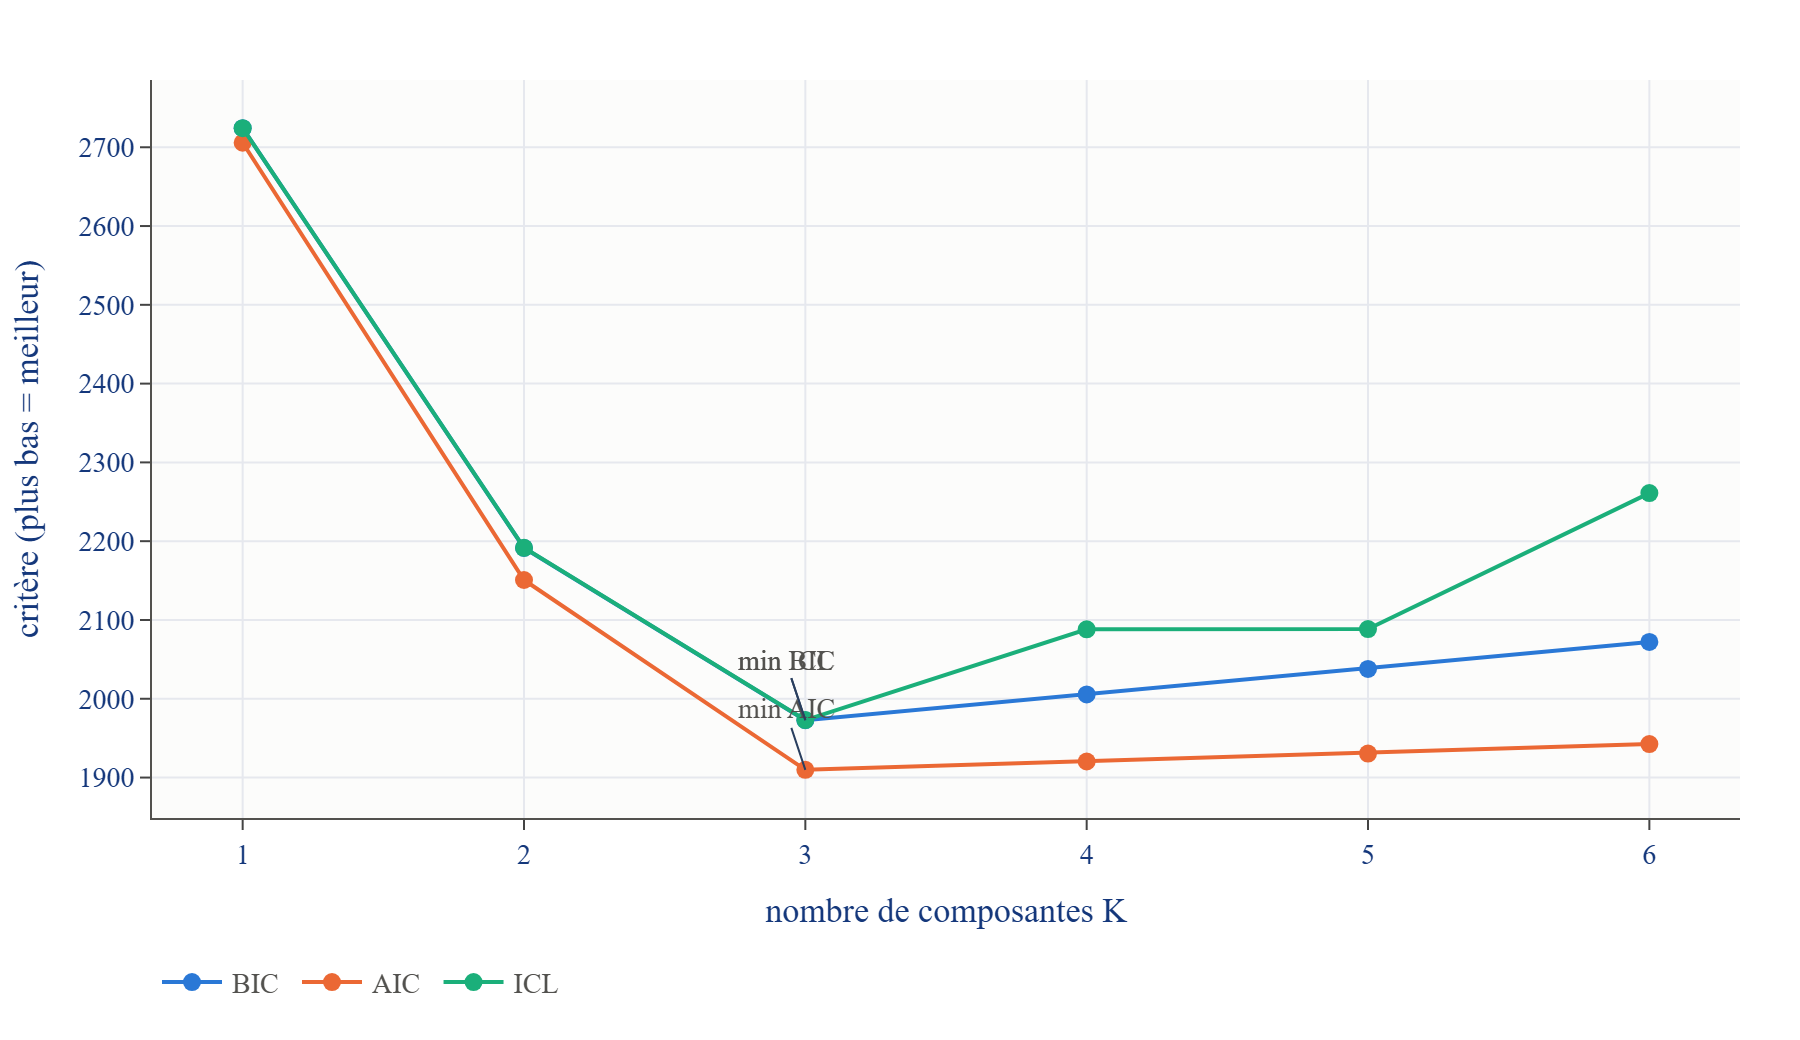
\includegraphics[width=0.85\textwidth]{figures/fig02.png}
\caption{Critères BIC et AIC de l'EM classique en fonction du nombre de composantes K, sur le jeu de données à trois groupes réels.}
\label{fig:2_1}
\end{figure}
\tableauGenere{ill_bic_aic}
Le BIC est minimal à $K = 3$ (1972,74), comme l'ICL (1972,96) et l'AIC (1909,78) ; de $K = 3$ à $K = 6$, la log-vraisemblance ne gagne plus que 1,67 (tableau~\ref{tab:ill_bic_aic}). Les trois critères retrouvent donc le nombre de groupes générateurs. Cette figure fixe la \emph{baseline pertinente} pour la suite : la comparaison utile n'est pas « EM avec $K = 6$ imposé contre VB avec $K_{\max} = 6$ » (situation volontairement défavorable à l'EM, section \ref{sec:res_k3}), mais « EM avec $K$ choisi par BIC ou ICL contre VB ». Le coût de cette baseline (un ajustement EM par valeur de $K$ et par initialisation) est comparé au coût d'un ajustement variationnel en temps total, jamais en proportion du nombre de valeurs de $K$ testées.

\subsection{EM à $K = 6$ imposé et EM variationnel à $K_{\max} = 6$}\label{sec:res_em_k6}\label{sec:res_vb_k6}\label{sec:res_partition}
L'EM classique est ajusté avec $K=6$ composantes, l'EM variationnel avec $K_{\max}=6$, des priors empiriques et un prior de Dirichlet de concentration $\alpha_0 = 1/K$ (vingt initialisations et critère d'arrêt commun pour les deux). Le tableau~\ref{tab:ill_k6} donne, pour chaque ajustement, le nombre de composantes actives (seuil $N_k/N \geq 1\,\%$), l'ARI et la silhouette, calculés sur les affectations à la composante de responsabilité maximale, et le nombre d'itérations ; les partitions et les poids finaux figurent aux figures~\ref{fig:2_3} et~\ref{fig:2_4}.

\tableauGenere{ill_k6}
\emph{Source : implémentation PyTorch (graine dérivée du rôle, annexe D) ; les temps sont ceux d'une exécution unique, le coût étant jugé par l'étape de chronométrage (HP4).}

L'EM garde ses six composantes actives, avec un ARI de 0,995 (initialisation k-means) et de 0,990 (initialisation aléatoire), en 233 itérations : les composantes excédentaires ne captent que quelques points. Il n'a aucun mécanisme interne pour reconnaître que $K=6$ est surestimé ; un balayage de $K$ par BIC ou ICL le fait (section~\ref{sec:selection_modele}). Le VB à priors empiriques ne garde que trois composantes actives, les trois autres s'éteignant, et retrouve exactement la partition génératrice (ARI de 1,000) en 21 itérations. Avec des priors diffus ($\beta_0 = 10^{-3}$, $W_0 = I$), il garde aussi trois composantes et le même ARI, mais en 538 itérations (487 avec une initialisation par le prior) : sur ce jeu bien séparé, les priors changent la vitesse de convergence, pas la solution.

Quatre remarques encadrent cette lecture. (1) La comparaison est défavorable à l'EM par construction, puisque son $K$ est imposé ; la comparaison pertinente, avec EM-BIC et EM-ICL, est celle des scénarios (section~\ref{sec:res_s1s3}). (2) L'élagage ne libère pas le VB du choix de $K$ : le nombre de composantes qu'il retient dépend de $K_{\max}$ et des priors, ce que mesurent les sections~\ref{sec:res_alpha0}, \ref{sec:res_scenarios} et~\ref{sec:res_s9s10}. (3) La silhouette dépend surtout du nombre de composantes et n'est pas utilisée comme preuve. (4) L'ELBO, calculée exactement (équation~\eqref{eq:1_31}), reste inférieure à la log-vraisemblance maximale de l'EM, comme l'exige la chaîne $\mathrm{ELBO} \leq \log p(X) \leq \max_{\theta} \log p(X \mid \theta)$ : elle intègre la pénalité de complexité due aux priors, et les deux quantités ne se comparent pas comme deux scores d'ajustement (figure~\ref{fig:2_7}). Le nombre d'itérations, mesuré au même critère d'arrêt, n'est pas une propriété intrinsèque des algorithmes, et le temps n'est comparé qu'à critère et machine communs (sections~\ref{sec:res_scalabilite} et~\ref{sec:res_cout}).

\begin{figure}[H]
\centering
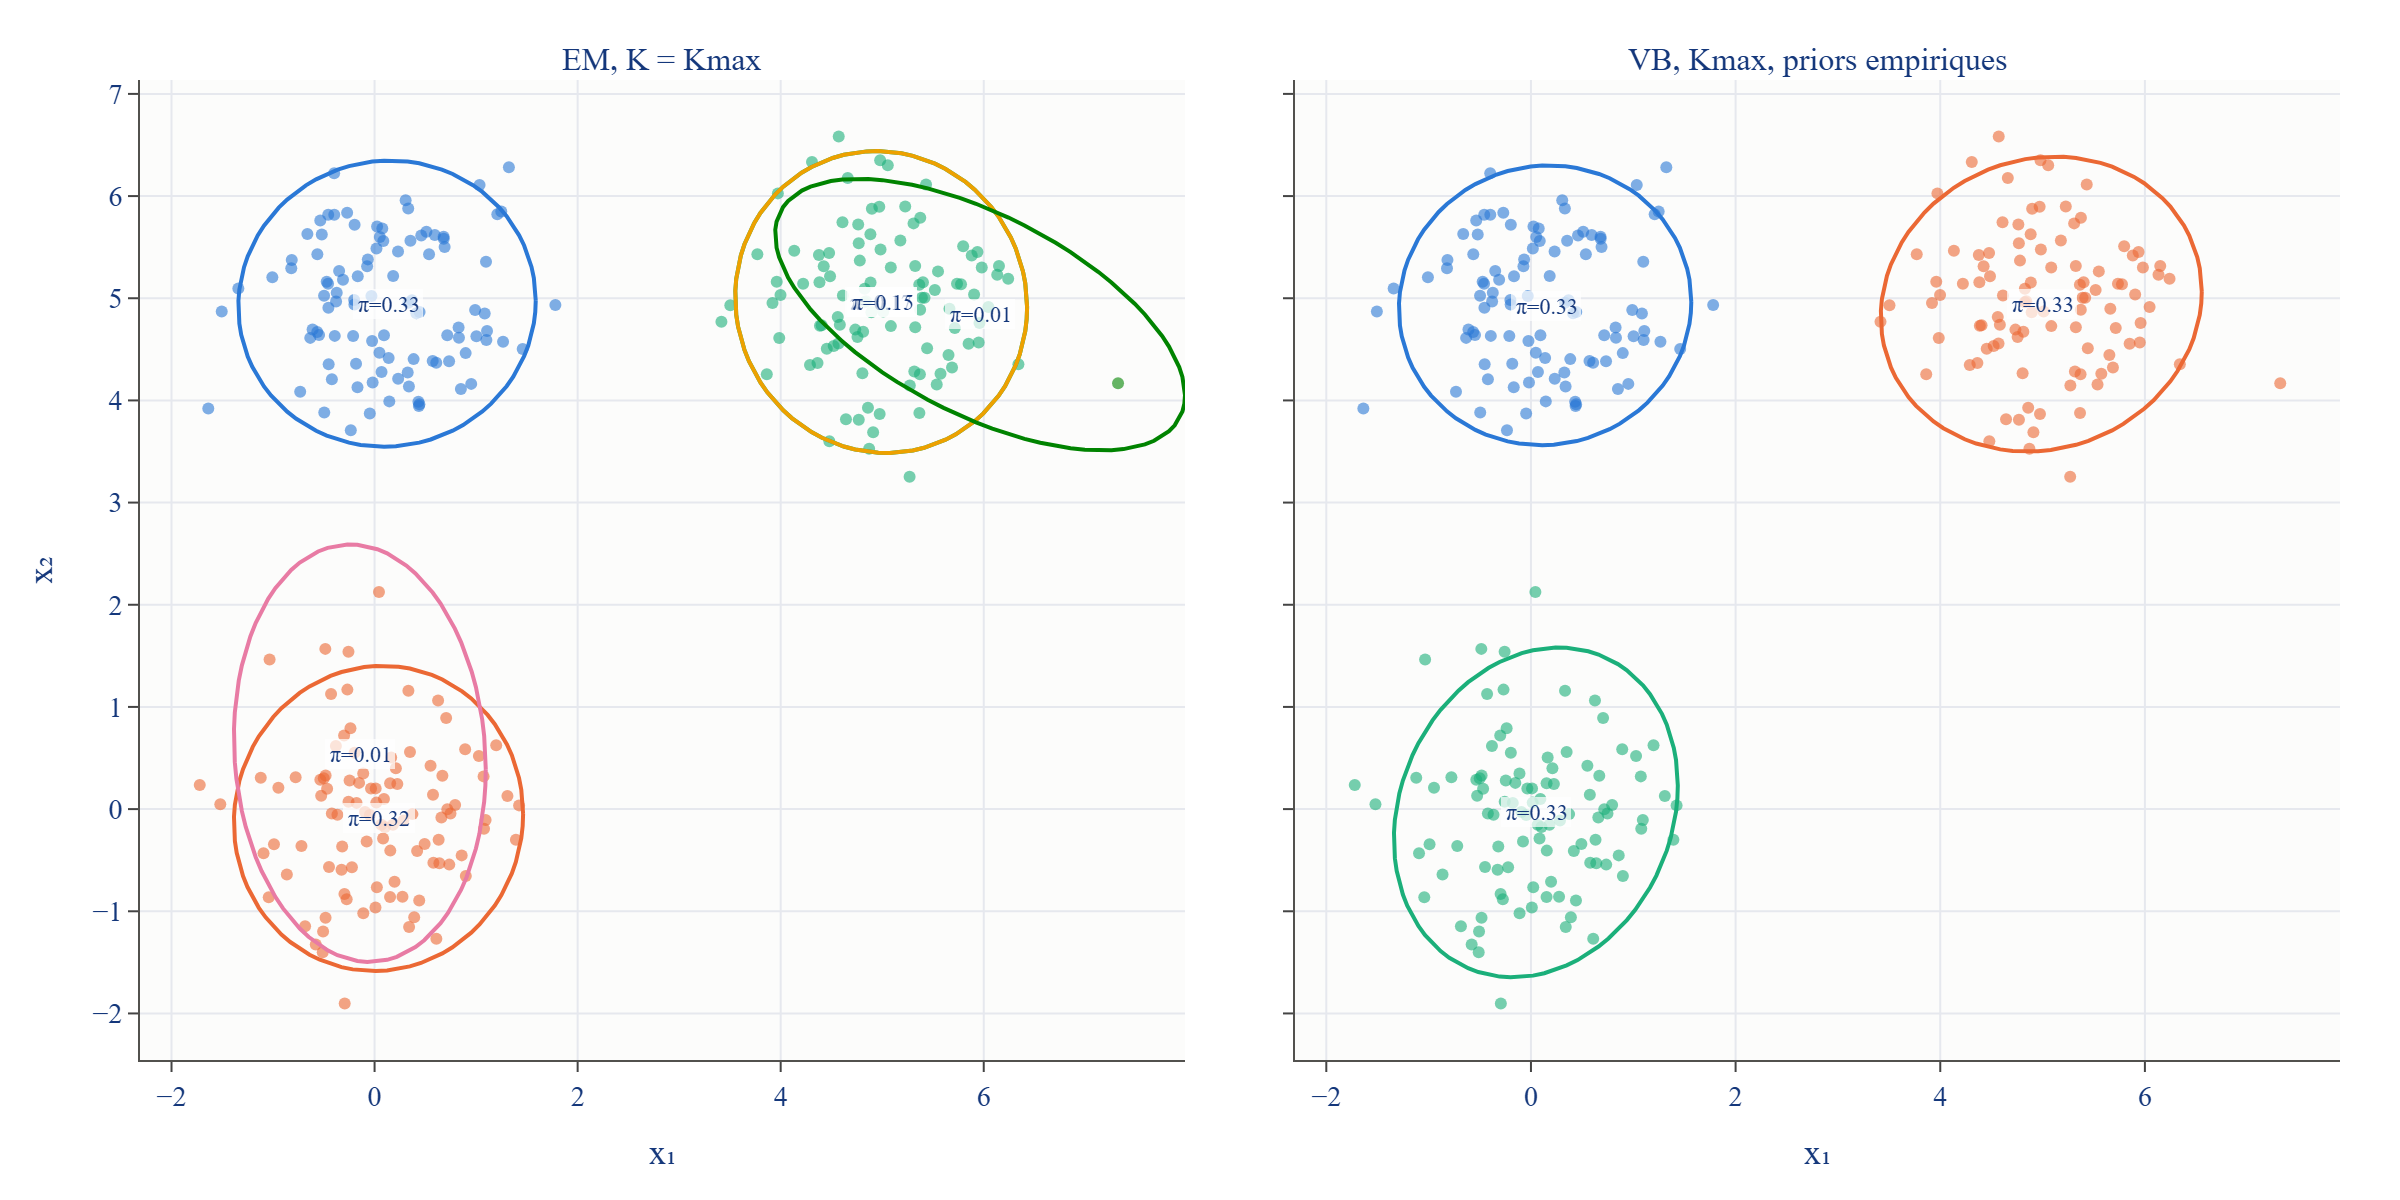
\includegraphics[width=0.95\textwidth]{figures/fig04.png}
\caption{Partition obtenue avec six composantes : une couleur par composante, ellipses de covariance à deux écarts-types, croix aux centres. À gauche, l'EM classique conserve ses six composantes ; à droite, l'EM variationnel n'en retient que trois (les composantes élaguées figurent en gris dans la légende).}
\label{fig:2_3}
\end{figure}
\begin{figure}[H]
\centering
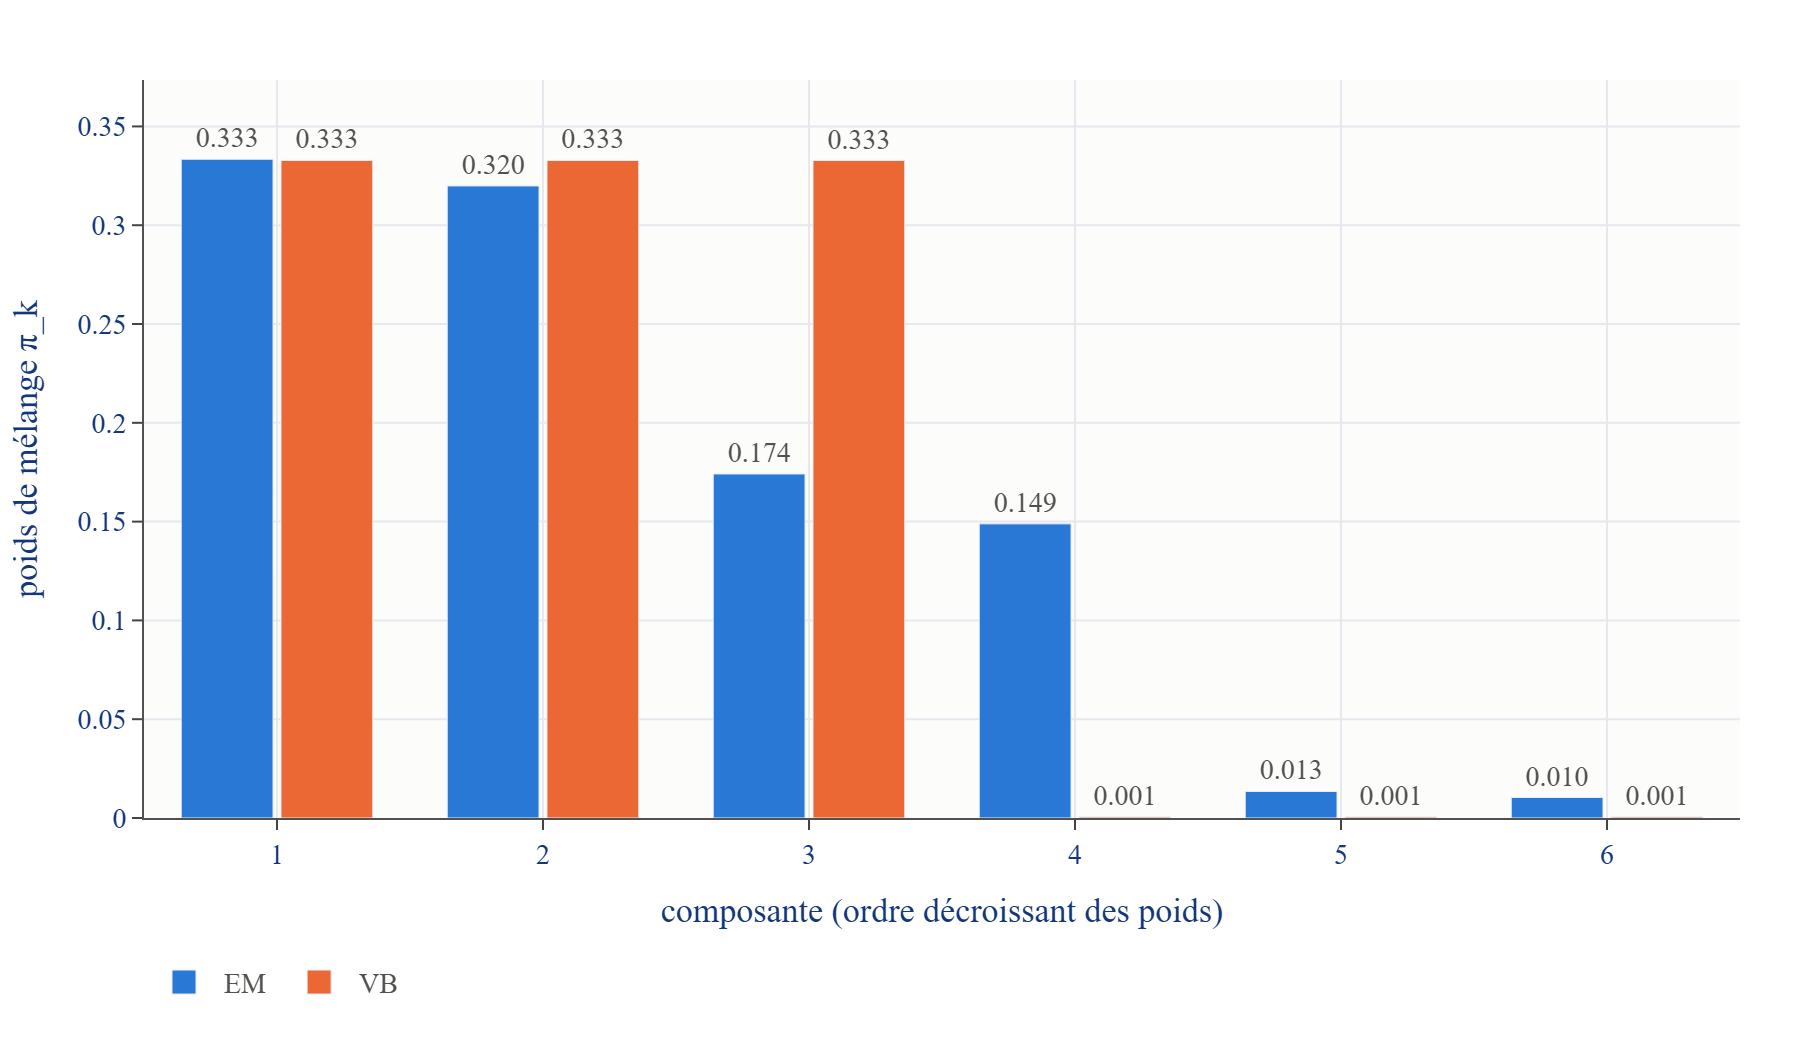
\includegraphics[width=0.85\textwidth]{figures/fig05.png}
\caption{Poids de mélange $\pi _{k}$ finaux pour les six composantes : EM classique et EM variationnel. Le contraste traduit le mécanisme d'élagage bayésien décrit à la section~\ref{sec:elagage}.}
\label{fig:2_4}
\end{figure}
\subsection{Sensibilité au choix du prior de Dirichlet ($\alpha _{0}$)}\label{sec:res_alpha0}
La section~\ref{sec:elagage} a montré que la concentration $\alpha_0$ du prior de Dirichlet contrôle l'élagage. Pour le vérifier, l'expérience de la section \ref{sec:res_vb_k6} est répétée en faisant varier $\alpha_0$ sur une grille logarithmique de neuf valeurs, de 0,001 à 10 (deux par décade), toutes choses égales par ailleurs ($K_{\max}=6$, mêmes données, vingt initialisations), pour les deux jeux de priors (tableau~\ref{tab:ill_alpha0}, figure~\ref{fig:2_5}). Cette grille est grossière autour de la zone de transition : la grille S8, en fin de section, la complète.

\tableauGenere{ill_alpha0}
\begin{figure}[H]
\centering
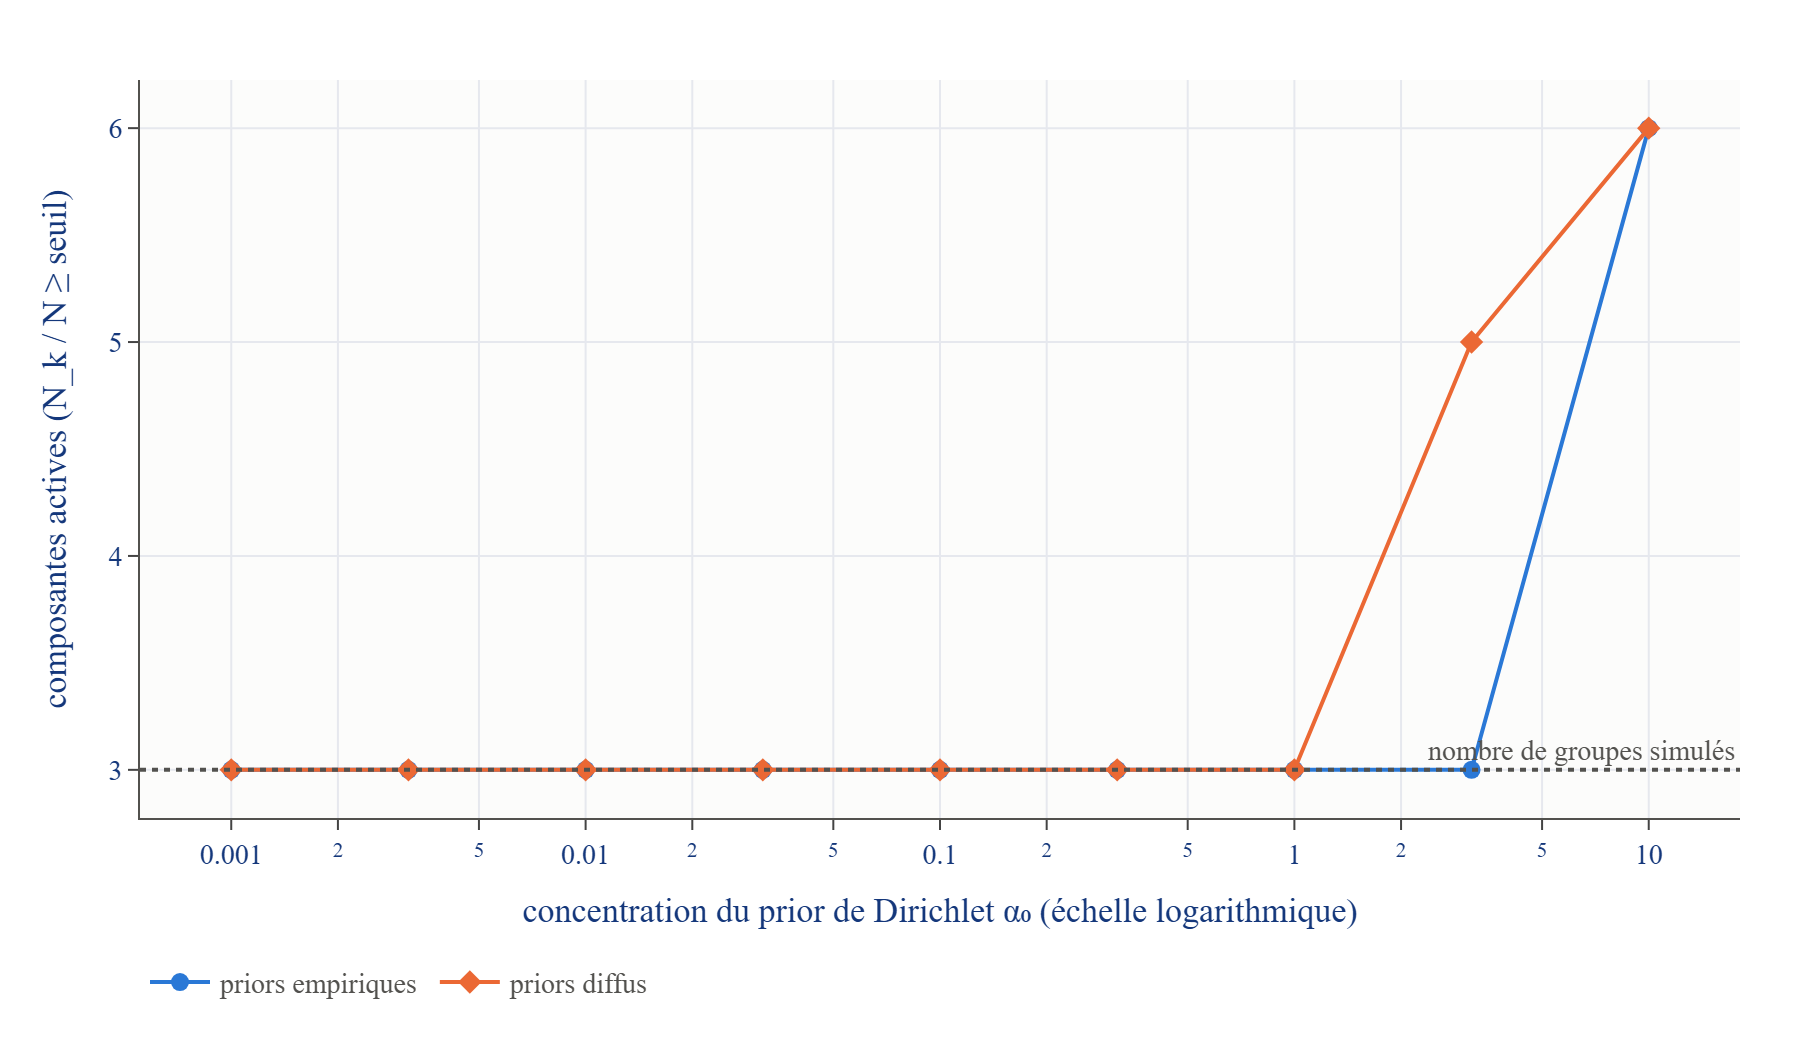
\includegraphics[width=0.85\textwidth]{figures/fig06.png}
\caption{Nombre de composantes actives en fonction de la concentration $\alpha _{0}$ du prior de Dirichlet (échelle logarithmique), pour les deux jeux de priors. Le mécanisme d'élagage disparaît lorsque $\alpha _{0}$ devient grand.}
\label{fig:2_5}
\end{figure}
Avec les priors empiriques, le VB garde trois composantes actives (ARI 1,000) de $\alpha_0 = 0{,}001$ à $\alpha_0 \approx 3{,}16$, puis six à $\alpha_0 = 10$ (ARI 0,990). Avec les priors diffus, la transition vient plus tôt : cinq composantes actives à $\alpha_0 \approx 3{,}16$ (ARI 0,751) et six à $\alpha_0 = 10$ (ARI 0,571). En dessous de 1, $\alpha_0$ ne change rien sur ce jeu (tableau~\ref{tab:ill_alpha0}). Le nombre de composantes actives dépend du seuil d'activité et n'est pas, à lui seul, une mesure de la qualité de la partition.

\textbf{Grille fine autour du seuil $d/2$ (S8, descriptif).}\label{sec:res_s8} Les seuils théoriques de Rousseau et Mengersen~\cite{rousseau2011} valent $d/2 = 2{,}5$ (covariance pleine), 2 (diagonale) et 1,5 (sphérique) en dimension 2 ; ils portent sur le posterior exact, non sur le champ moyen. La grille $\alpha_0 \in \{1;\,1{,}5;\,2;\,2{,}5;\,3;\,5;\,10\}$ est évaluée pour les trois types de covariance sur 110 réplications (fichier \texttt{S8\_alpha0.csv} du dépôt du mémoire, annexe A ; pour les covariances non pleines, le critère d'arrêt est une approximation, section~\ref{sec:impl_vb}). Le nombre moyen de composantes actives reste proche de 3 pour les petites valeurs de $\alpha_0$ et vaut 6 pour $\alpha_0 \geq 5$ dans les trois cas. La montée commence plus tôt quand la covariance est plus contrainte : en sphérique, il atteint 3,69 dès $\alpha_0 = 2$ et 4,97 à $\alpha_0 = 2{,}5$ ; en diagonale, 3,63 à $\alpha_0 = 2{,}5$ et 4,85 à $\alpha_0 = 3$ ; en covariance pleine, il ne vaut encore que 3,26 à $\alpha_0 = 3$. L'ordre des transitions (sphérique, diagonale, pleine) est celui des seuils $d/2$, mais chaque transition devient nette au-dessus de son seuil, d'un demi-point au moins ; toutes les exécutions ont convergé. Ce résultat ne confirme ni ne réfute la théorie, qui porte sur le posterior exact : il situe seulement, pour le champ moyen, la zone où $\alpha_0$ pilote $\hat K$.

\subsection{Étude de la scalabilité computationnelle}\label{sec:res_scalabilite}
Le temps des deux algorithmes est mesuré en faisant varier $N$ (à $D=2$) et $D$ (à $N=2001$, un jeu distinct de celui de la grille en $N$), vingt répétitions par configuration (médiane), une initialisation et le critère d'arrêt commun ; le tableau~\ref{tab:chronometrage} et la figure~\ref{fig:2_6} séparent le temps jusqu'au modèle final, le nombre d'itérations et le coût par itération.

\tableauGenere{chronometrage}
\begin{figure}[H]
\centering
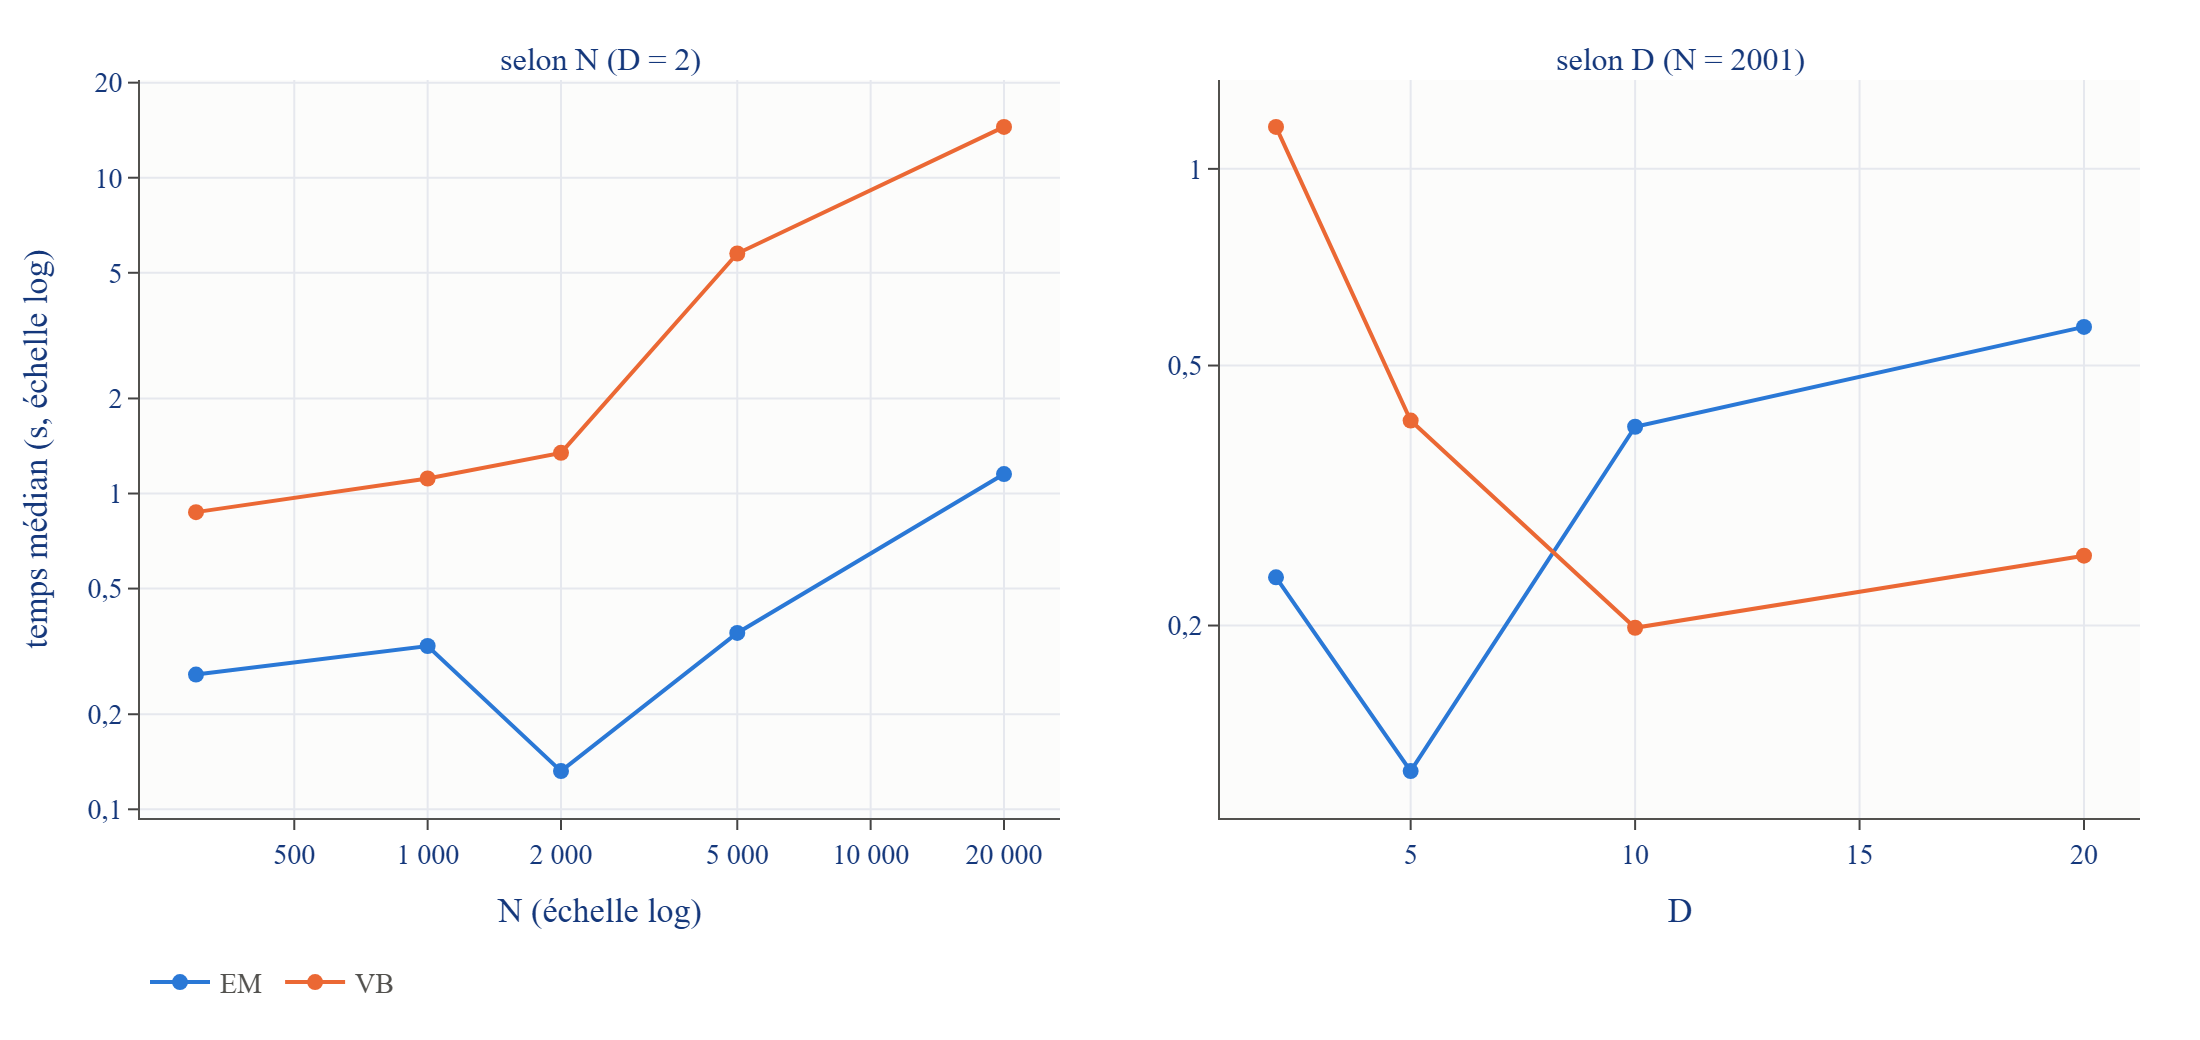
\includegraphics[width=0.95\textwidth]{figures/fig07.png}
\caption{Temps d'exécution des deux algorithmes en fonction du nombre d'observations N (à gauche, échelles logarithmiques) et de la dimension D (à droite). Les étiquettes donnent le rapport du temps variationnel au temps classique.}
\label{fig:2_6}
\end{figure}
\emph{Source : implémentation PyTorch (CPU, un processus, graine dérivée du rôle, annexe D).}

Les deux grandeurs doivent être lues séparément. Le \emph{coût par itération} du VB vaut de 1,1 à 2,2 fois celui de l'EM (colonne « Rapport par itération ») ; ce rapport diminue quand $N$ croît (2,22 à $N = 300$, 1,13 à $N = 20\,000$) et reste entre 1,6 et 1,9 quand $D$ varie. Le \emph{temps jusqu'au modèle final} est le produit de ce coût par le nombre d'itérations, qui varie dans un sens ou dans l'autre : le rapport des temps va de 0,45 ($D = 20$, où le VB s'arrête en 58 itérations contre 198 pour l'EM) à 15,9 ($N = 5\,000$). À $N = 5\,000$ et $N = 20\,000$, le VB atteint le plafond de 1 800 étapes dans 11 et 20 répétitions sur 20 (fichier \texttt{chronometrage\_brut.csv}) : son critère d'arrêt n'y est pas atteint et son temps n'est qu'une borne inférieure. Ces mesures sont propres à une machine, à une implémentation et à $D \leq 20$ : la conclusion « le VB est $x$ fois plus lent » n'est pas retenue, et la question utile, le temps total d'un pipeline EM-BIC contre un VB, est traitée à la section \ref{sec:res_cout}.

\subsection{Cas de référence : nombre de composantes correctement spécifié (K = 3)}\label{sec:res_k3}
L'expérience est répétée avec $K = 3$, le nombre exact de groupes, pour sortir du cas défavorable à l'EM (tableau~\ref{tab:ill_k3}).

\tableauGenere{ill_k3}
À $K = 3$, les deux algorithmes retrouvent exactement la partition génératrice (ARI 1,000, silhouette 0,753), en 4 itérations pour l'EM et 2 pour le VB (tableau~\ref{tab:ill_k3}) : sans surestimation de $K$, ils ne se distinguent pas sur ce jeu. Le choix entre les deux ne peut donc pas s'appuyer sur le seul contraste à $K$ surestimé : il dépend de la confiance dans $K$, du besoin d'incertitude et du budget de calcul (tableau~\ref{tab:2_17}).

\subsection{Convergence de l'ELBO}\label{sec:res_elbo}
La figure~\ref{fig:2_7} retrace l'ELBO, calculée exactement à chaque itération (équation~\ref{eq:1_31}), du modèle à $K_{\max}=6$ de la section \ref{sec:res_vb_k6} (même appel que le tableau~\ref{tab:ill_k6}), et la log-vraisemblance de l'EM à $K=6$.

\begin{figure}[H]
\centering
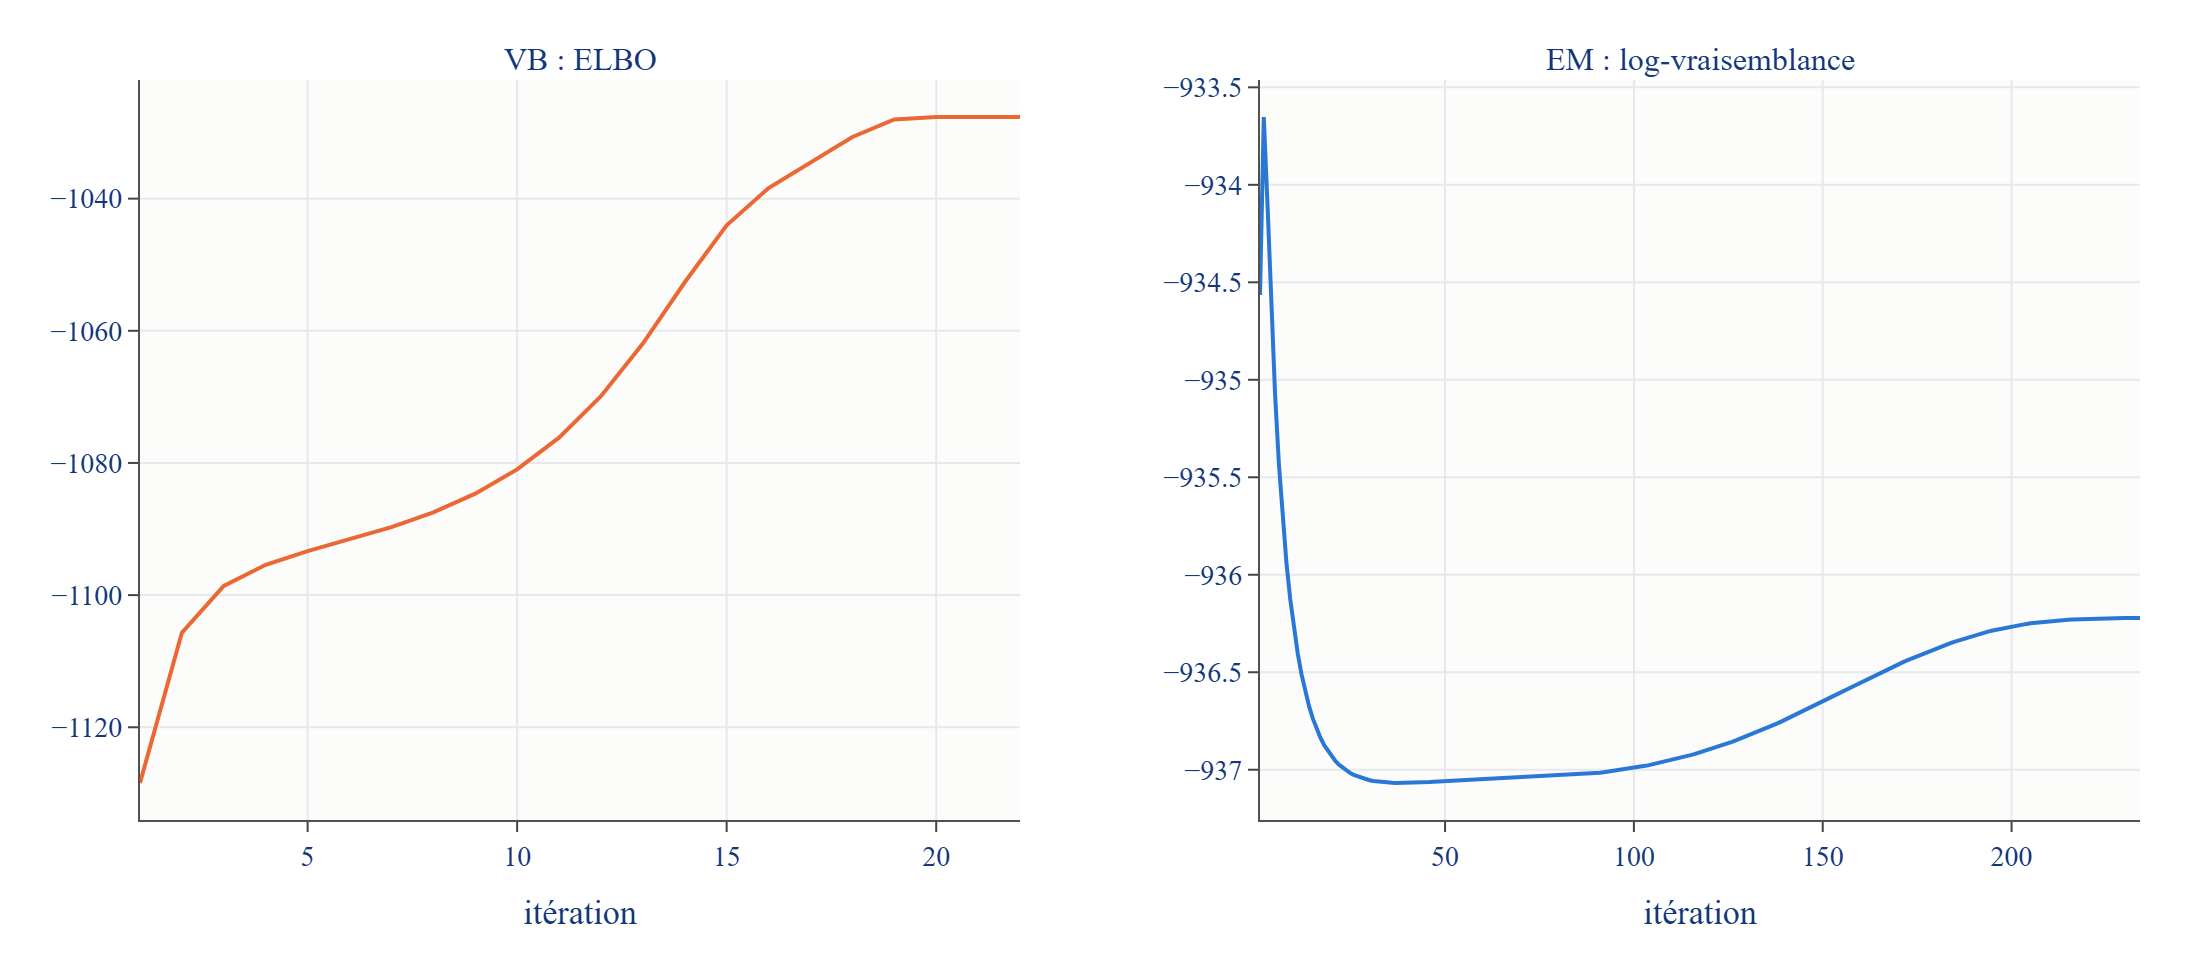
\includegraphics[width=0.95\textwidth]{figures/fig08.png}
\caption{Évolution de l'ELBO (EM variationnel, à gauche) et de la log-vraisemblance (EM classique, à droite) en fonction du nombre d'itérations. Les deux courbes sont croissantes, conformément aux garanties théoriques des sections~\ref{sec:formulation_mathematique_complete}.f et \ref{sec:calcul_elbo}.}
\label{fig:2_7}
\end{figure}
L'ELBO ne décroît jamais, conformément à la garantie de la section~\ref{sec:calcul_elbo} ; cette monotonie, l'inégalité $\mathrm{ELBO} \leq \log p(X) \leq \ell(\hat\theta)$ et l'égalité de Neal et Hinton, $F(q^*, \theta) = \ell(\theta)$ après l'étape E, sont vérifiées numériquement sur l'EM \emph{sans} régularisation ($\varepsilon = 0$), puisque l'ajout de $\varepsilon I$ change l'étape M et rompt la garantie de monotonie ; les relances dont une covariance cesse d'être définie positive sont comptées à part (tableau~\ref{tab:validation_proprietes}). Sur 20 graines, aucune baisse de la log-vraisemblance ni de l'ELBO n'est observée, l'écart maximal à l'égalité de Neal et Hinton vaut $3{,}81 \times 10^{-6}$, et l'ELBO reste inférieure à la log-vraisemblance maximale pour toutes les graines ; aucune relance n'échoue, mais un quart des EM sans régularisation sont dégénérés. Ces propriétés sont aussi couvertes par des tests unitaires. L'ELBO fait l'essentiel de son gain dans les premières itérations.

\subsection{Robustesse à l'initialisation}\label{sec:res_init}
Pour mesurer la sensibilité propre de chaque algorithme à l'initialisation, l'expérience est répétée avec une seule initialisation par exécution, pour 110 graines et deux stratégies : k-means et aléatoire ($K$ points tirés au hasard, sections~\ref{sec:formulation_mathematique_complete}.a et \ref{sec:formulation_de_l_em_variationnel}.d).

\tableauGenere{ill_initialisation}
\begin{figure}[H]
\centering
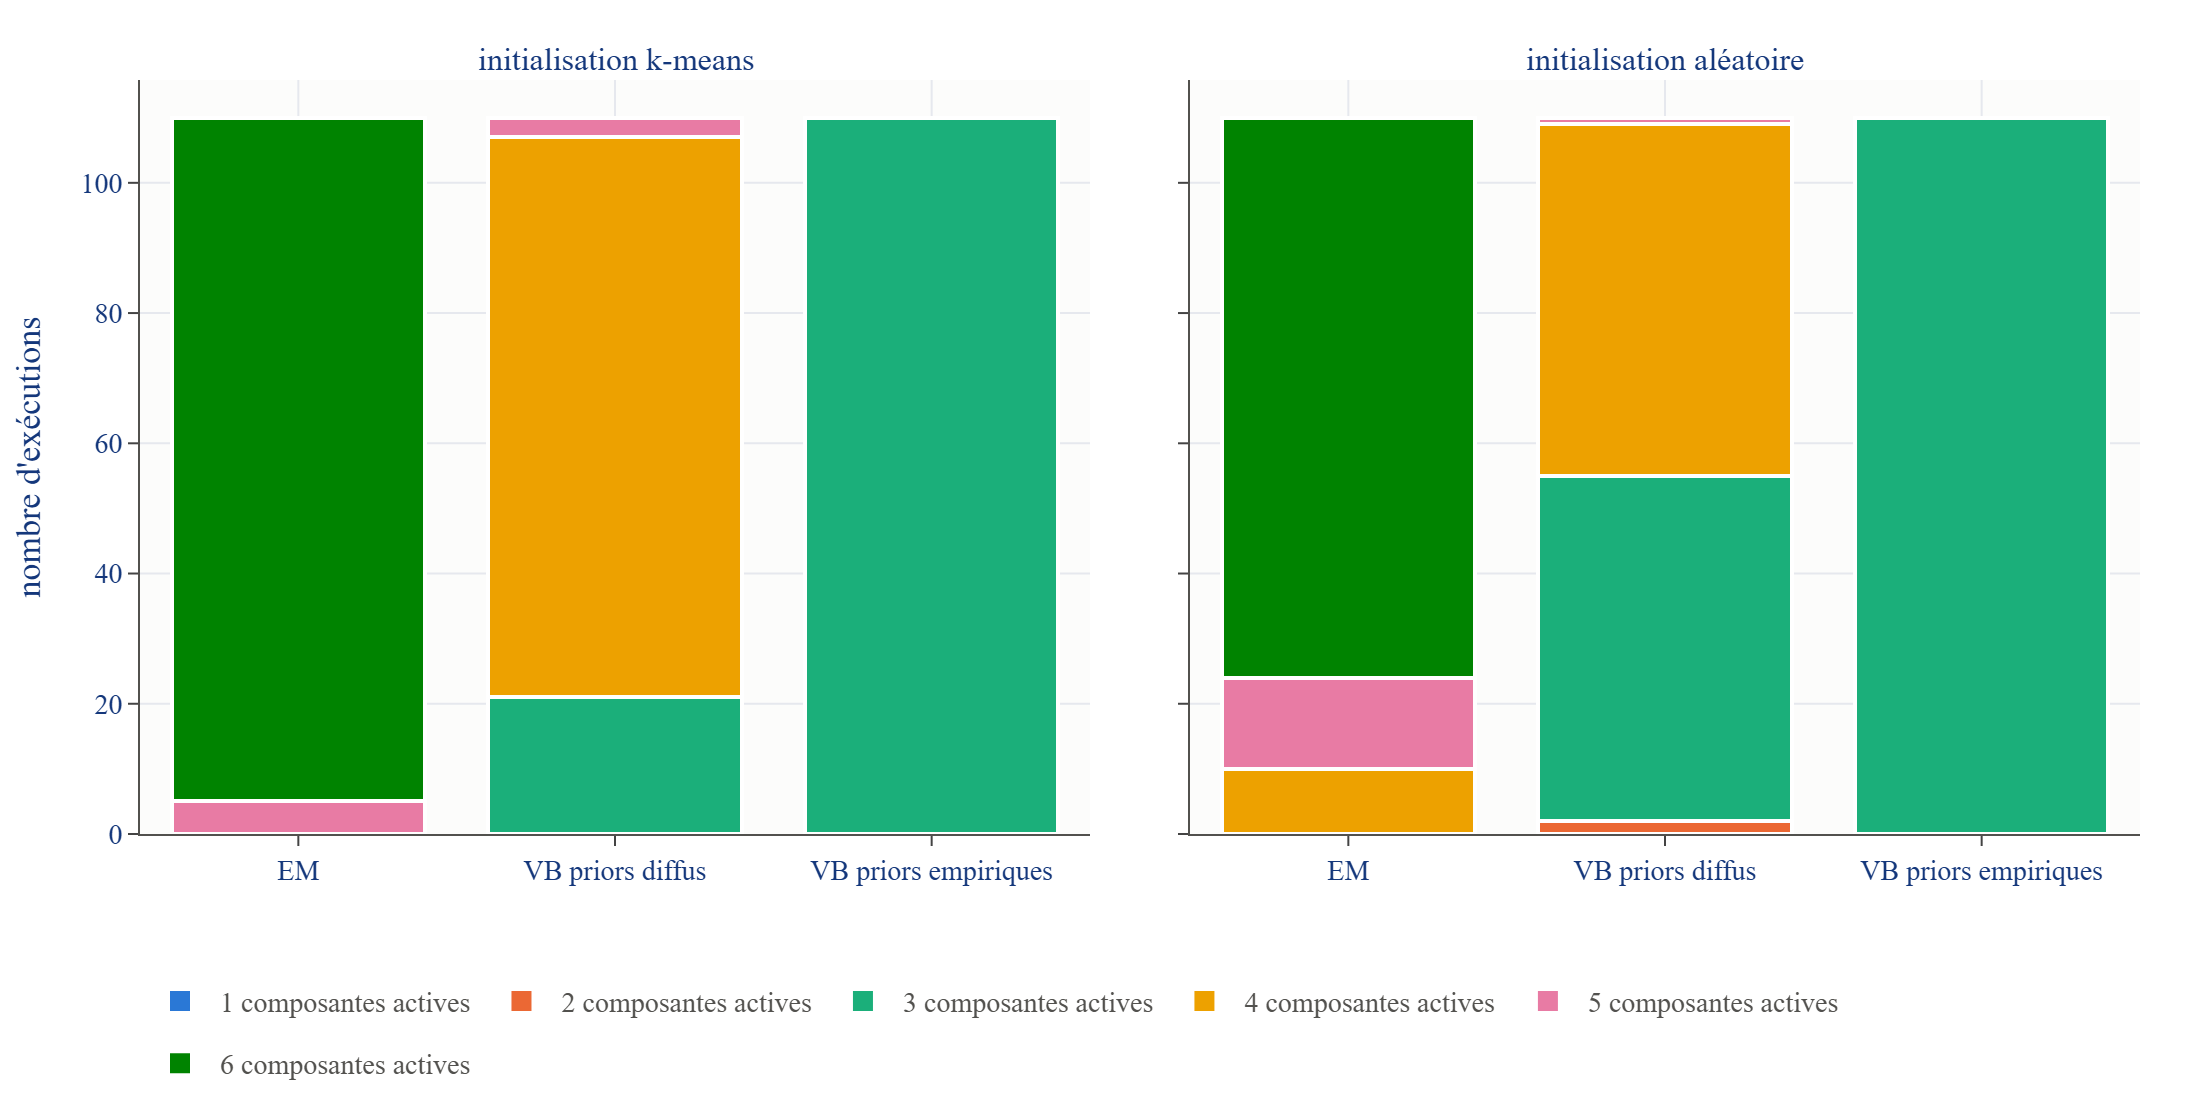
\includegraphics[width=0.95\textwidth]{figures/fig09.png}
\caption{Répartition du nombre de composantes actives selon l'algorithme et la stratégie d'initialisation (110 exécutions chacune, une initialisation par exécution).}
\label{fig:2_8}
\end{figure}
Avec les priors empiriques, le VB garde trois composantes actives dans les 110 exécutions, quelle que soit l'initialisation. Avec les priors diffus, il en garde le plus souvent trois ou quatre : avec l'initialisation k-means, 21 exécutions sur 110 en gardent trois, 86 quatre et 3 cinq ; avec l'initialisation aléatoire, 2 en gardent deux, 53 trois, 54 quatre et 1 cinq (tableau~\ref{tab:ill_initialisation}). L'élagage dépend donc de l'initialisation quand les priors sont diffus. L'EM à $K = 6$ n'élimine aucune composante, mais certaines passent sous le seuil d'activité de 1 \% : c'est le cas dans 5 exécutions sur 110 avec l'initialisation k-means et dans 24 avec l'initialisation aléatoire.

\subsection{Sensibilité au type de covariance}\label{sec:res_covariance}
L'expérience de la section \ref{sec:res_partition} est reproduite pour les quatre formes de covariance (pleine, liée, diagonale, sphérique) ; pour le VB, les trois dernières, non dérivées au chapitre~\ref{chap:fondements}, utilisent un prior de Wishart partagé ou des priors Gamma conjugués sur les précisions (tableau~\ref{tab:ill_covariance}).

\tableauGenere{ill_covariance}
\begin{figure}[H]
\centering
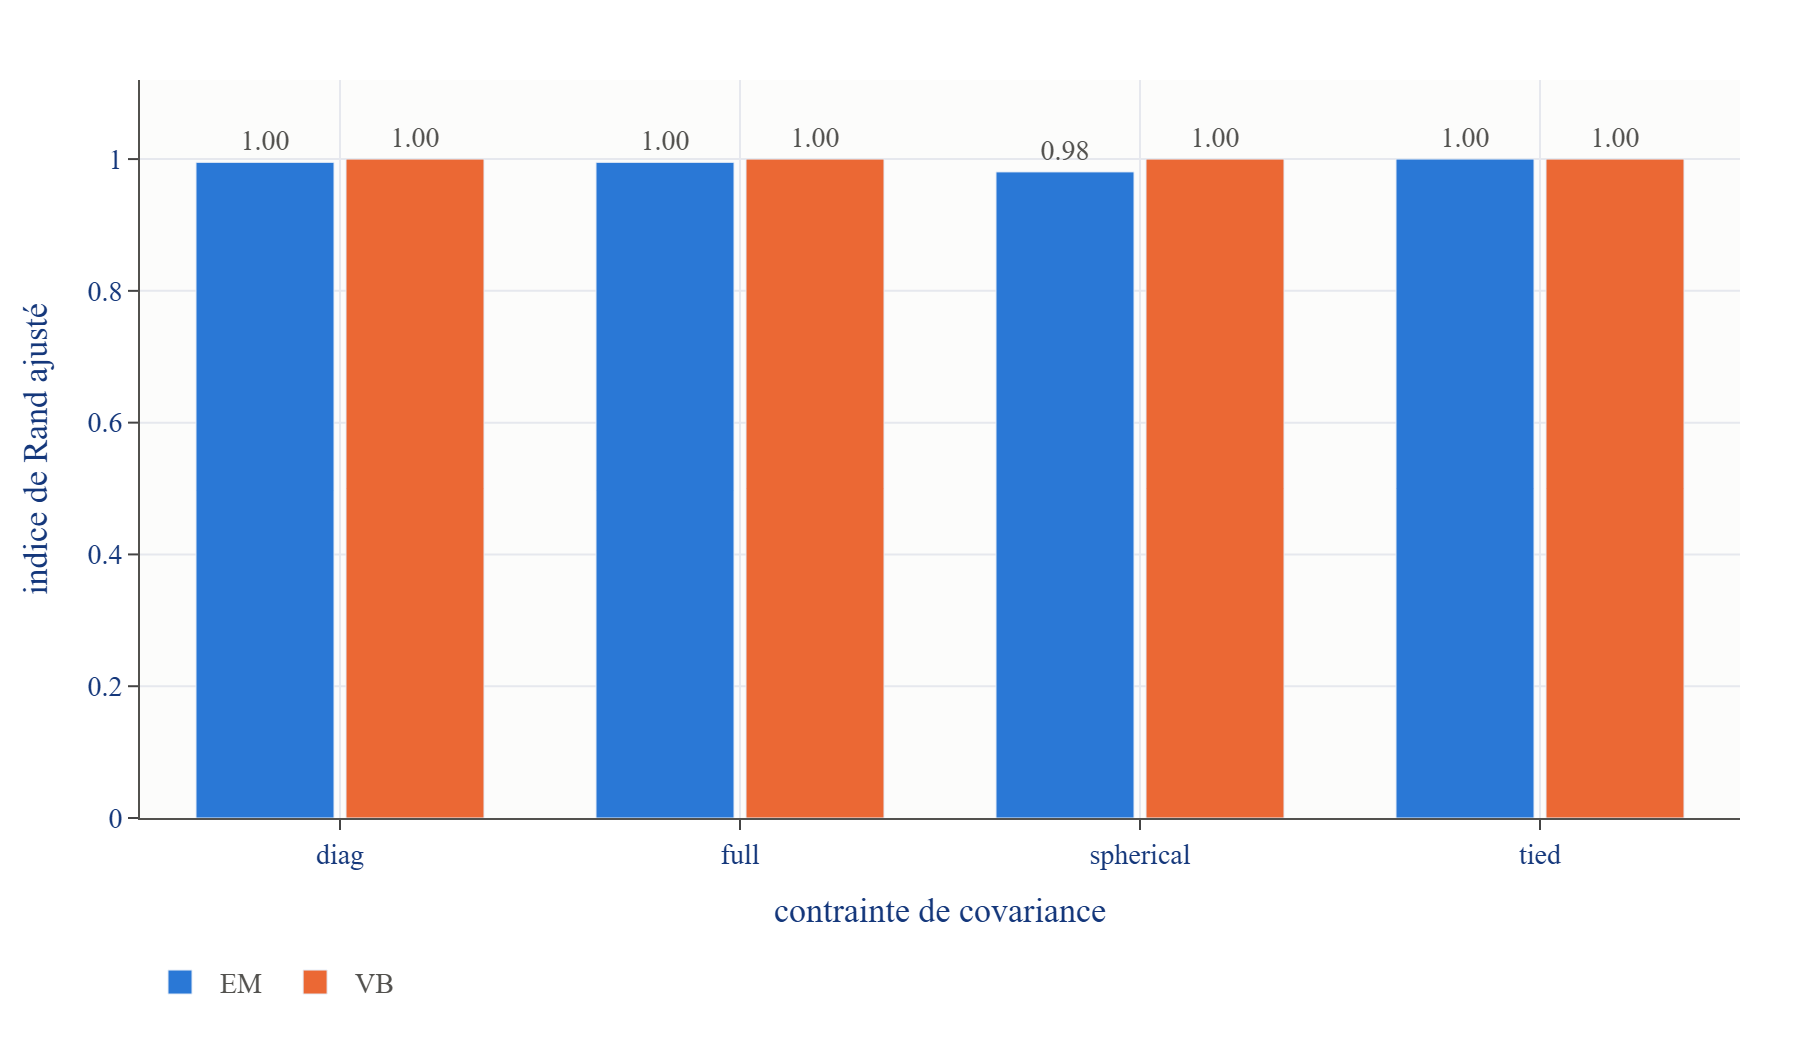
\includegraphics[width=0.85\textwidth]{figures/fig10.png}
\caption{Indice de Rand ajusté selon la contrainte imposée sur la covariance (K = 6 imposé).}
\label{fig:2_9}
\end{figure}
Le VB à priors empiriques garde trois composantes actives et retrouve la partition génératrice (ARI 1,000) pour les quatre formes de covariance. L'EM à $K = 6$ garde six composantes actives en covariance pleine et liée, cinq en diagonale et en sphérique, avec un ARI de 0,981 à 1,000 (tableau~\ref{tab:ill_covariance}). Pour tied, diag et spherical, le VB utilise un critère d'arrêt approché (somme des log-normalisations de l'étape E, ELBO privée du terme KL sur $\theta$, non nécessairement monotone) et l'ELBO de ces variantes n'est pas dérivée : un élagage éventuel est donc observé \emph{avec une approximation}, et son extension à ces formes reste à valider en dérivant l'ELBO de chaque variante (section \ref{sec:impl_vb}).

\subsection{Validation sur un jeu de données réel (Iris)}\label{sec:res_iris}
Pour sortir du cadre synthétique, l'expérience est reproduite sur le jeu Iris de Fisher~\cite{fisher1936} : $N=150$ observations en dimension $D=4$, trois espèces, mesures brutes en centimètres (non standardisées), avec $K=6$ imposé, puis $K=3$ (tableau~\ref{tab:ill_iris}).

\tableauGenere{ill_iris}
\emph{Source : Iris de Fisher~\cite{fisher1936}, fichier UCI Machine Learning Repository ; calculs de l'auteur.}

\begin{figure}[H]
\centering
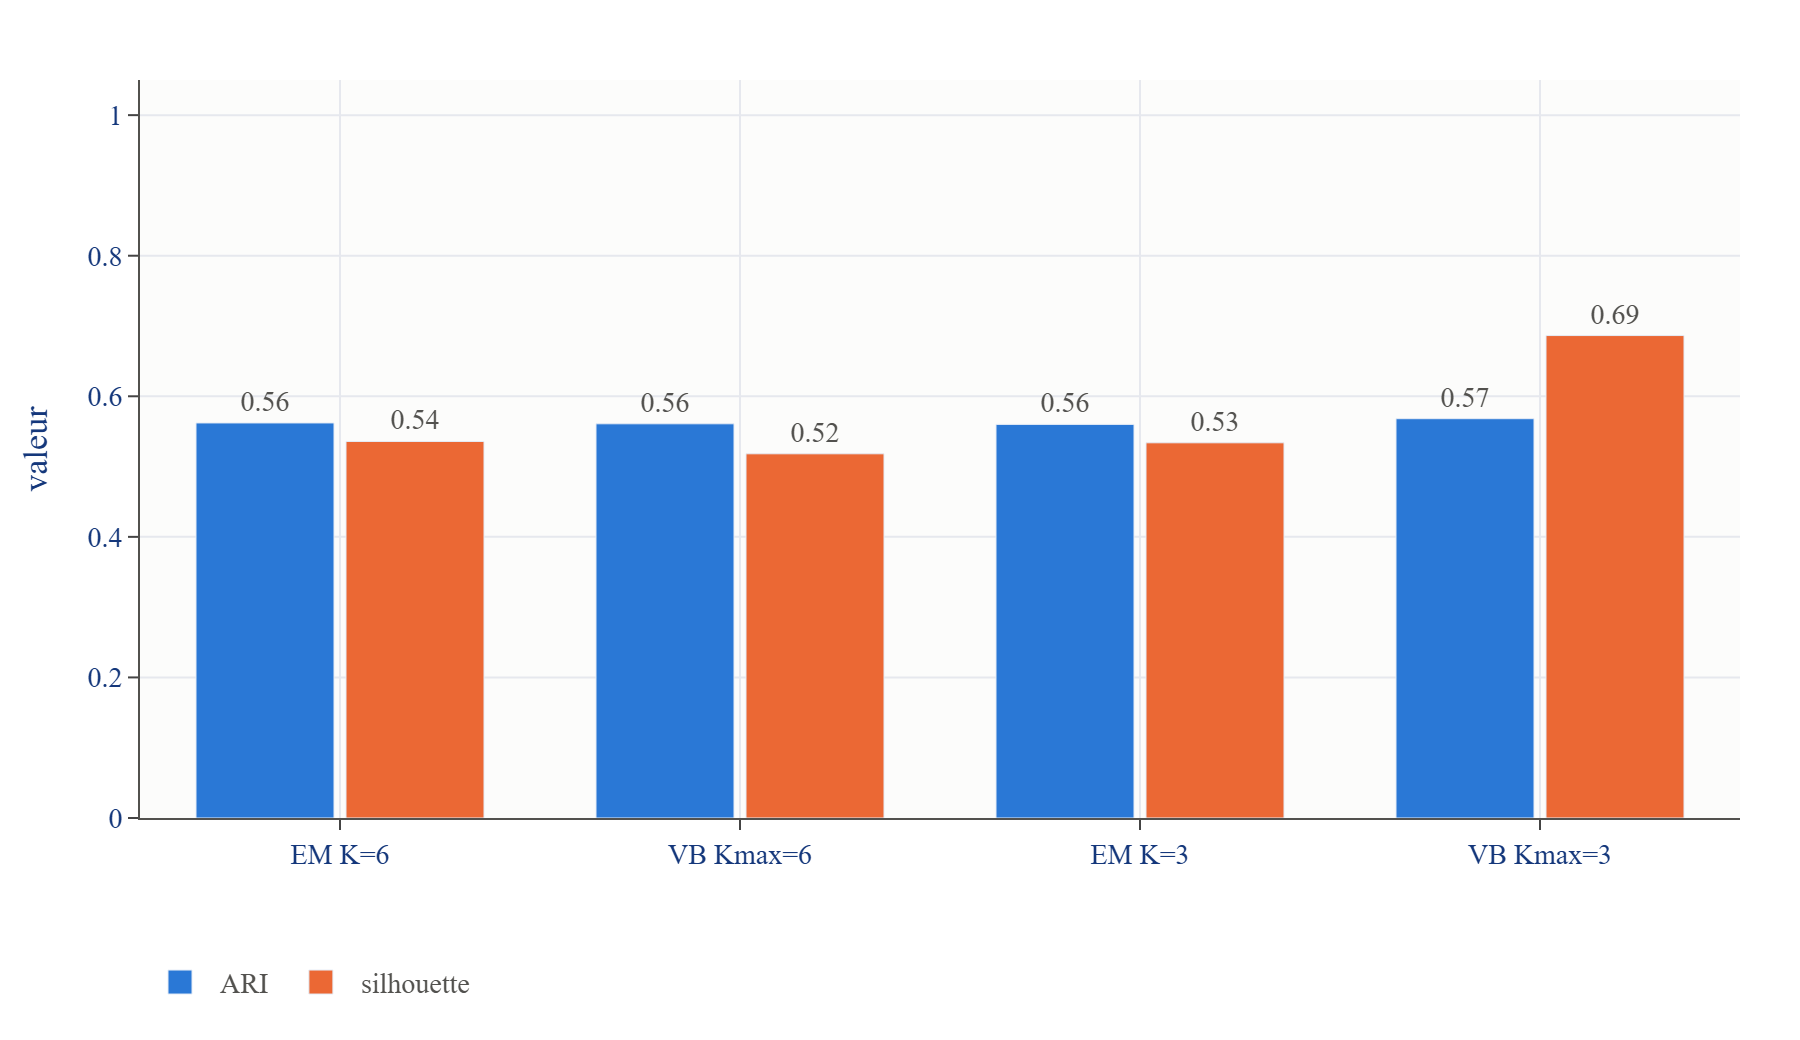
\includegraphics[width=0.85\textwidth]{figures/fig11.png}
\caption{Indice de Rand ajusté et silhouette sur le jeu Iris, selon l'algorithme et le nombre de composantes.}
\label{fig:2_10}
\end{figure}
Sur Iris, le VB à $K_{\max}=6$ garde trois composantes actives et obtient le même ARI que l'EM à $K=6$, qui garde ses six composantes (0,561 contre 0,562) ; l'EM à $K = 3$ obtient 0,560 (tableau~\ref{tab:ill_iris}). Les trois ajustements ne retrouvent qu'en partie les espèces, dont deux se chevauchent. Un point de méthode : avec $N=150$, $D=4$ et $K=6$ en covariance pleine, l'EM compte 89 paramètres libres pour 150 points ($6 \times 4$ moyennes, $6 \times 10$ termes de covariance, 5 poids), cas typique de singularité. L'ARI suppose que les étiquettes définissent les groupes à retrouver ; si deux espèces se chevauchent, la log-vraisemblance hors échantillon et la comparaison avec EM-BIC sont plus informatives.

Avec $K_{\max} = 3$, le VB ne garde que deux composantes actives et obtient un ARI de 0,568, proche des autres, avec une silhouette plus élevée (0,686 contre 0,518 à $K_{\max} = 6$). Le nombre de composantes retenu par le VB dépend donc de $K_{\max}$ (trois pour $K_{\max} = 6$, deux pour $K_{\max} = 3$), sans que l'ARI change notablement.

\subsection{Sensibilité aux valeurs aberrantes}\label{sec:res_aberrantes}
Dix points aberrants (environ 3 \%), tirés uniformément dans une boîte trois fois plus large que l'étendue des données et centrée sur elles, ont été ajoutés au jeu de données de la section \ref{sec:donnees_reference}, puis les deux algorithmes ont été ajustés avec K = 6 sur ce jeu augmenté (N = 310).

\tableauGenere{ill_aberrantes}
Cette expérience, fondée sur un seul tirage, n'est pas un test de robustesse : elle illustre le comportement des composantes en présence d'aberrations. Sur le jeu augmenté, l'EM à $K=6$ et le VB obtiennent tous deux un ARI hors aberrations de 1,000 et gardent quatre composantes actives. La trace maximale des covariances (25,2 pour l'EM, 81,6 pour le VB) suggère qu'une composante large absorbe les aberrations ; la plus petite composante active pèse 0,013 pour l'EM et 0,034 pour le VB (tableau~\ref{tab:ill_aberrantes}). Le test de robustesse, répliqué et comparé à EM-BIC, est le scénario S7 (section~\ref{sec:decisions_et_lecture}).

\section{Scénarios confirmatoires S1 à S10}\label{sec:res_scenarios}
Cette section présente les résultats des scénarios dont le plan est décrit à la section~\ref{sec:scenarios_plan} : chevauchement, déséquilibre et sous-estimation de $K$ (S1 à S3), queues épaisses, dimension et petit effectif (S4 à S6), aberrations (S7).\label{sec:res_s1s3}\label{sec:res_s4s6}\label{sec:res_s7} Les moyennes par bras sur les réplications (ARI, $\hat K$, log-vraisemblance de test, part d'ajustements dégénérés) sont archivées dans le dépôt du mémoire (annexe A) (\texttt{scenarios\_resume.csv}) ; les décisions des tests déclarés (TOST ou Wilcoxon exact, correction de Holm sur la famille des scénarios) figurent au tableau~\ref{tab:decisions_scenarios} et à la figure~\ref{fig:scenarios_decisions}, et leur lecture, rattachée aux hypothèses de recherche, suit. Le taux d'ajustements dégénérés de S6 est celui de l'EM \emph{régularisé} par $\varepsilon I$ (section~\ref{sec:impl_em}) ; il ne dit rien de l'EM non régularisé.

\subsection{Décisions et lecture}\label{sec:decisions_et_lecture}
\tableauGenere{decisions_scenarios}
\textbf{Synthèse des scénarios.} La lecture détaillée de chaque décision (estimation, intervalle, probabilité critique de Holm, verdict) est archivée dans le dépôt du mémoire (annexe A). Quand les groupes sont bien séparés (4 et 5 écarts-types) ou contaminés par des aberrations (S7, neuf combinaisons de proportion et d'amplitude), le VB et l'EM-BIC sont équivalents à la marge de 0,05 d'ARI ; neuf de ces onze équivalences tiennent encore à la moitié de la marge (tableau~\ref{tab:sensibilite_marges}). Quand les groupes se chevauchent ou que la dimension croît, l'ARI du VB dépasse celui de l'EM-BIC : de 0,17 et 0,28 pour des groupes séparés de 2 et 3 écarts-types, de 0,28 et 0,79 pour $D = 10$ et $D = 20$. Le VB perd moins souvent la composante minoritaire (S2, écart de fréquence de $-0{,}25$) et produit moins d'ajustements dégénérés que l'EM à $K_{\max}$ à tous les effectifs (S6, de $-0{,}76$ à $N = 30$ à $-0{,}15$ à $N = 1\,000$). Quand $K$ est sous-estimé (S3), l'ARI du VB à $K_{\max} = 3$ dépasse celui de l'EM à $K = 3$ de 0,04 à 0,09, et l'équivalence n'est pas démontrée. Aucune décision n'est contraire aux hypothèses. Les différences en faveur du VB portent sur l'EM-BIC tel qu'il est mis en œuvre ici, en covariance pleine ; une explication probable, non testée, est que la pénalité du BIC, qui croît avec le nombre de paramètres, conduit l'EM-BIC à retenir trop peu de composantes en dimension élevée ou quand les groupes se chevauchent.

\subsection{Plan factoriel sur les priors et seuil d'activité (S9 et S10, descriptifs)}\label{sec:res_s9s10}
Le plan factoriel fait varier $\alpha_0$, $\beta_0$, $\nu_0$ et l'échelle de $W_0$ ; la part de variance du nombre de composantes actives expliquée par chaque facteur est rapportée (tableau~\ref{tab:S9_variance}). Le scénario S10 montre la sensibilité du nombre de composantes actives au seuil (0,5 \%, 1 \%, 5 \% de $N$, et $N_k \geq 1$) : tant que ce nombre dépend du seuil, il ne constitue pas une mesure fiable de $\hat K$.

\tableauGenere{S9_variance}
\tableauGenere{S10_seuil}

\textbf{Lecture (S9 et S10). }$\alpha_0$ explique 69,1 \% de la variance du nombre de composantes actives, contre 4,1 \% pour $\beta_0$, 2,1 \% pour l'échelle de $W_0$ et 0,7 \% pour $\nu_0$, le résidu valant 24,1 \% (tableau~\ref{tab:S9_variance}). Le seuil d'activité compte peu loin de la transition : à $\alpha_0 = 1/6$, le nombre moyen de composantes vaut 3,02 au seuil $N_k \geq 1$ et 3,00 aux autres seuils ; à $\alpha_0 = 2{,}5$, il passe de 3,35 ($N_k \geq 1$) à 3,09 (5 \% de $N$) ; à $\alpha_0 = 10$, il vaut 6 à tous les seuils (tableau~\ref{tab:S10_seuil}).

\subsection{Coût de la sélection de $K$ en temps total}\label{sec:res_cout}
\tableauGenere{cout_selection}
Le rapport des temps médians entre le pipeline EM-BIC complet et un ajustement VB, à relances égales, est mesuré dans un seul processus sur les données de prix ; la décision HP4 (hypothèse RH5) est lue à la section~\ref{sec:res_prix}. Le coût par itération (tableau~\ref{tab:chronometrage}) et le temps total jusqu'au modèle final ne se confondent pas : seul le second compare des pipelines.

\section{Cas pratique : régimes de tension des prix alimentaires au Cameroun}\label{sec:res_prix}
Le cas, ses données et son plan sont décrits à la section~\ref{sec:prix_methodo}. Les résultats sont produits par le code depuis le magasin d'artefacts : modèle de référence (tableau~\ref{tab:prix_reference}), moyennes par plan, effectif et bras et relevés écartés par le nettoyage (dépôt du mémoire, annexe A), décisions (tableau~\ref{tab:decisions_prix} ; figure~\ref{fig:prix_decisions} en annexe H), ajustements sur toute la période d'apprentissage (tableau~\ref{tab:prix_complet}), comparaisons de prévision (tableau~\ref{tab:prix_dm}), régime de tension et probabilités d'alerte (tableau~\ref{tab:prix_alerte}, figures~\ref{fig:prix_alerte} et~\ref{fig:prix_alerte_mois}), confrontation aux épisodes datés (tableau~\ref{tab:prix_episodes}, figure~\ref{fig:prix_carte_alerte}). La sélection du nombre de régimes est illustrée en annexe H (figure~\ref{fig:prix_selection}).

\tableauGenere{prix_reference}
\tableauGenere{decisions_prix}
\tableauGenere{prix_complet}
\tableauGenere{prix_dm}
\tableauGenere{prix_alerte}

\begin{figure}[H]
\centering
\IfFileExists{figures/prix_alerte.png}{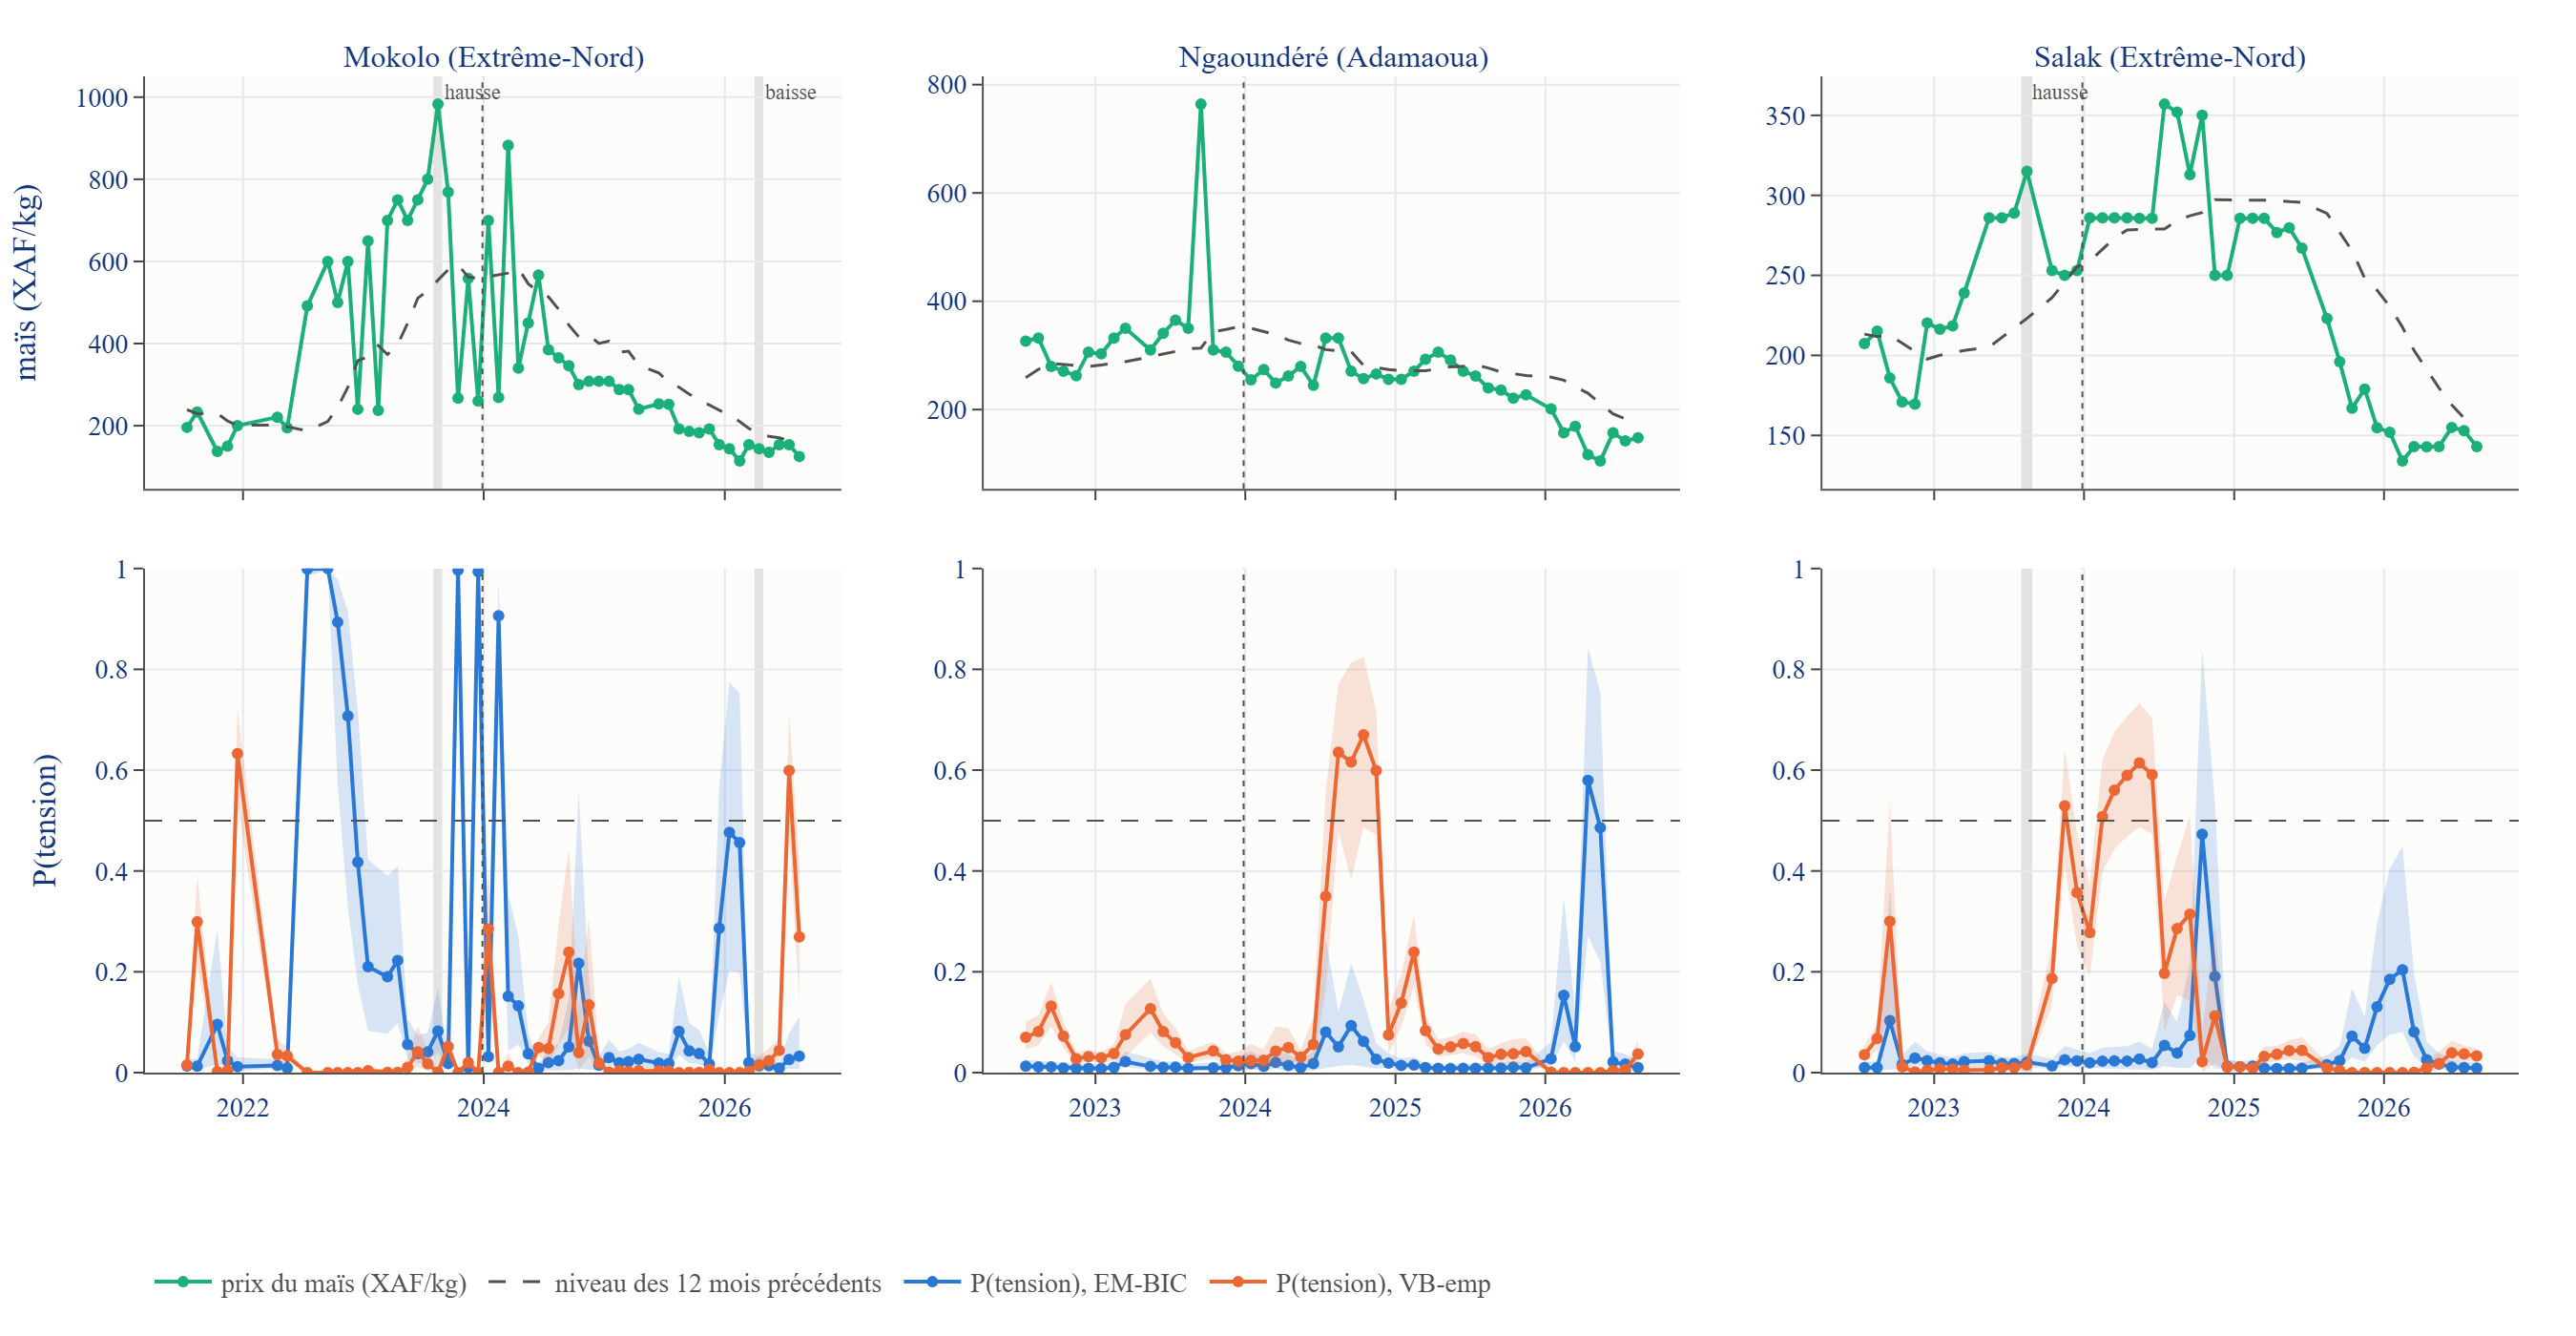
\includegraphics[width=\textwidth]{figures/prix_alerte.png}}{\fbox{\parbox{0.8\textwidth}{\centering figure à générer (\texttt{python run.py --figures})}}}
\caption{Les trois marchés les plus suivis pendant la période de test. En haut : prix de détail du maïs (XAF/kg) et son niveau des douze mois précédents (tirets) ; l'écart entre les deux, en logarithme, est la variable du modèle. En bas : probabilité du régime de tension selon EM-BIC (bande : bootstrap à 90 \%) et selon le VB à priors empiriques (bande : crédibilité à 90 \%). Bandes grises : épisodes datés par les bulletins (hausse d'août 2023, baisse d'avril 2026) pour les marchés concernés. Trait pointillé vertical : fin de l'apprentissage.}
\label{fig:prix_alerte}
\end{figure}
\begin{figure}[H]
\centering
\IfFileExists{figures/prix_alerte_mois.png}{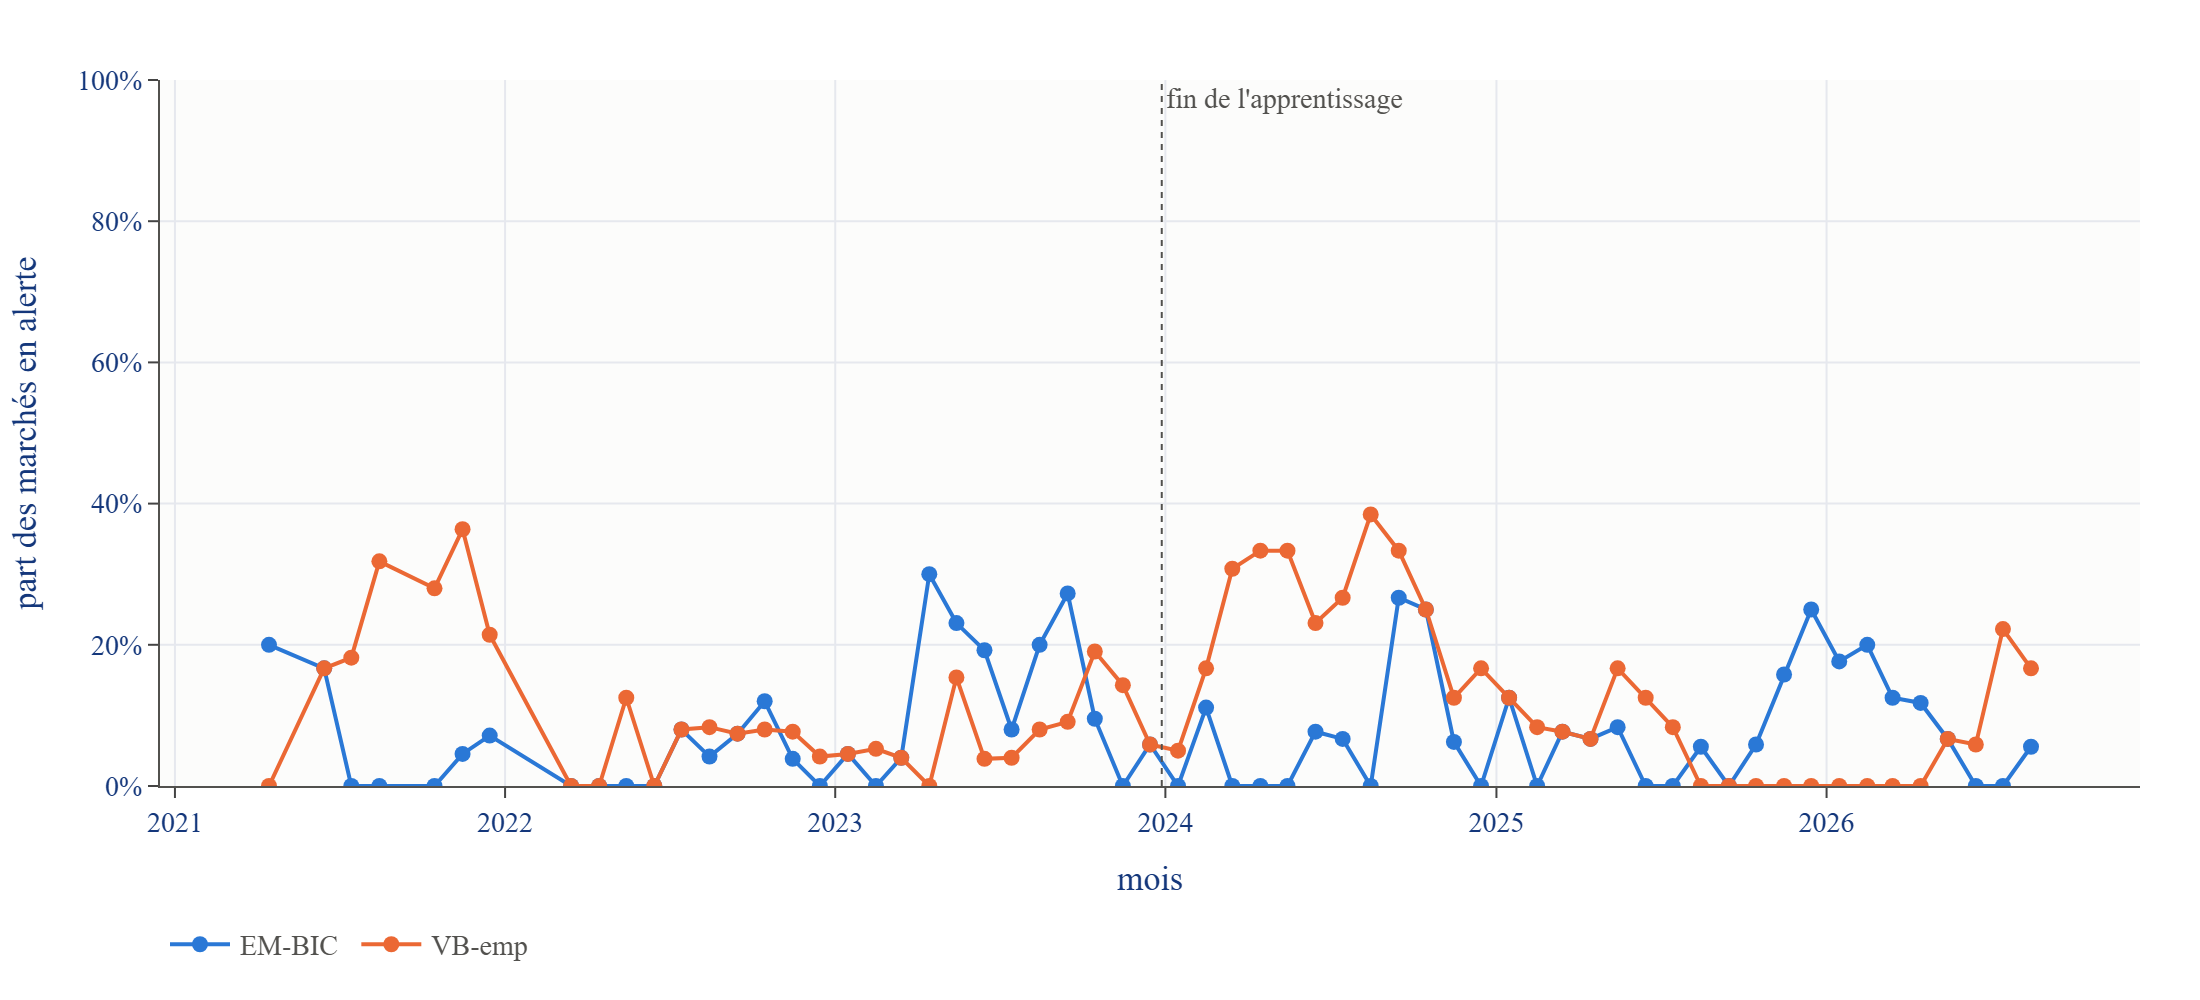
\includegraphics[width=0.95\textwidth]{figures/prix_alerte_mois.png}}{\fbox{\parbox{0.8\textwidth}{\centering figure à générer (\texttt{python run.py --figures})}}}
\caption{Part mensuelle des observations dont la probabilité de tension dépasse 0,5, tous marchés confondus, selon EM-BIC et le VB à priors empiriques.}
\label{fig:prix_alerte_mois}
\end{figure}
\begin{figure}[H]
\centering
\IfFileExists{figures/prix_carte_alerte.png}{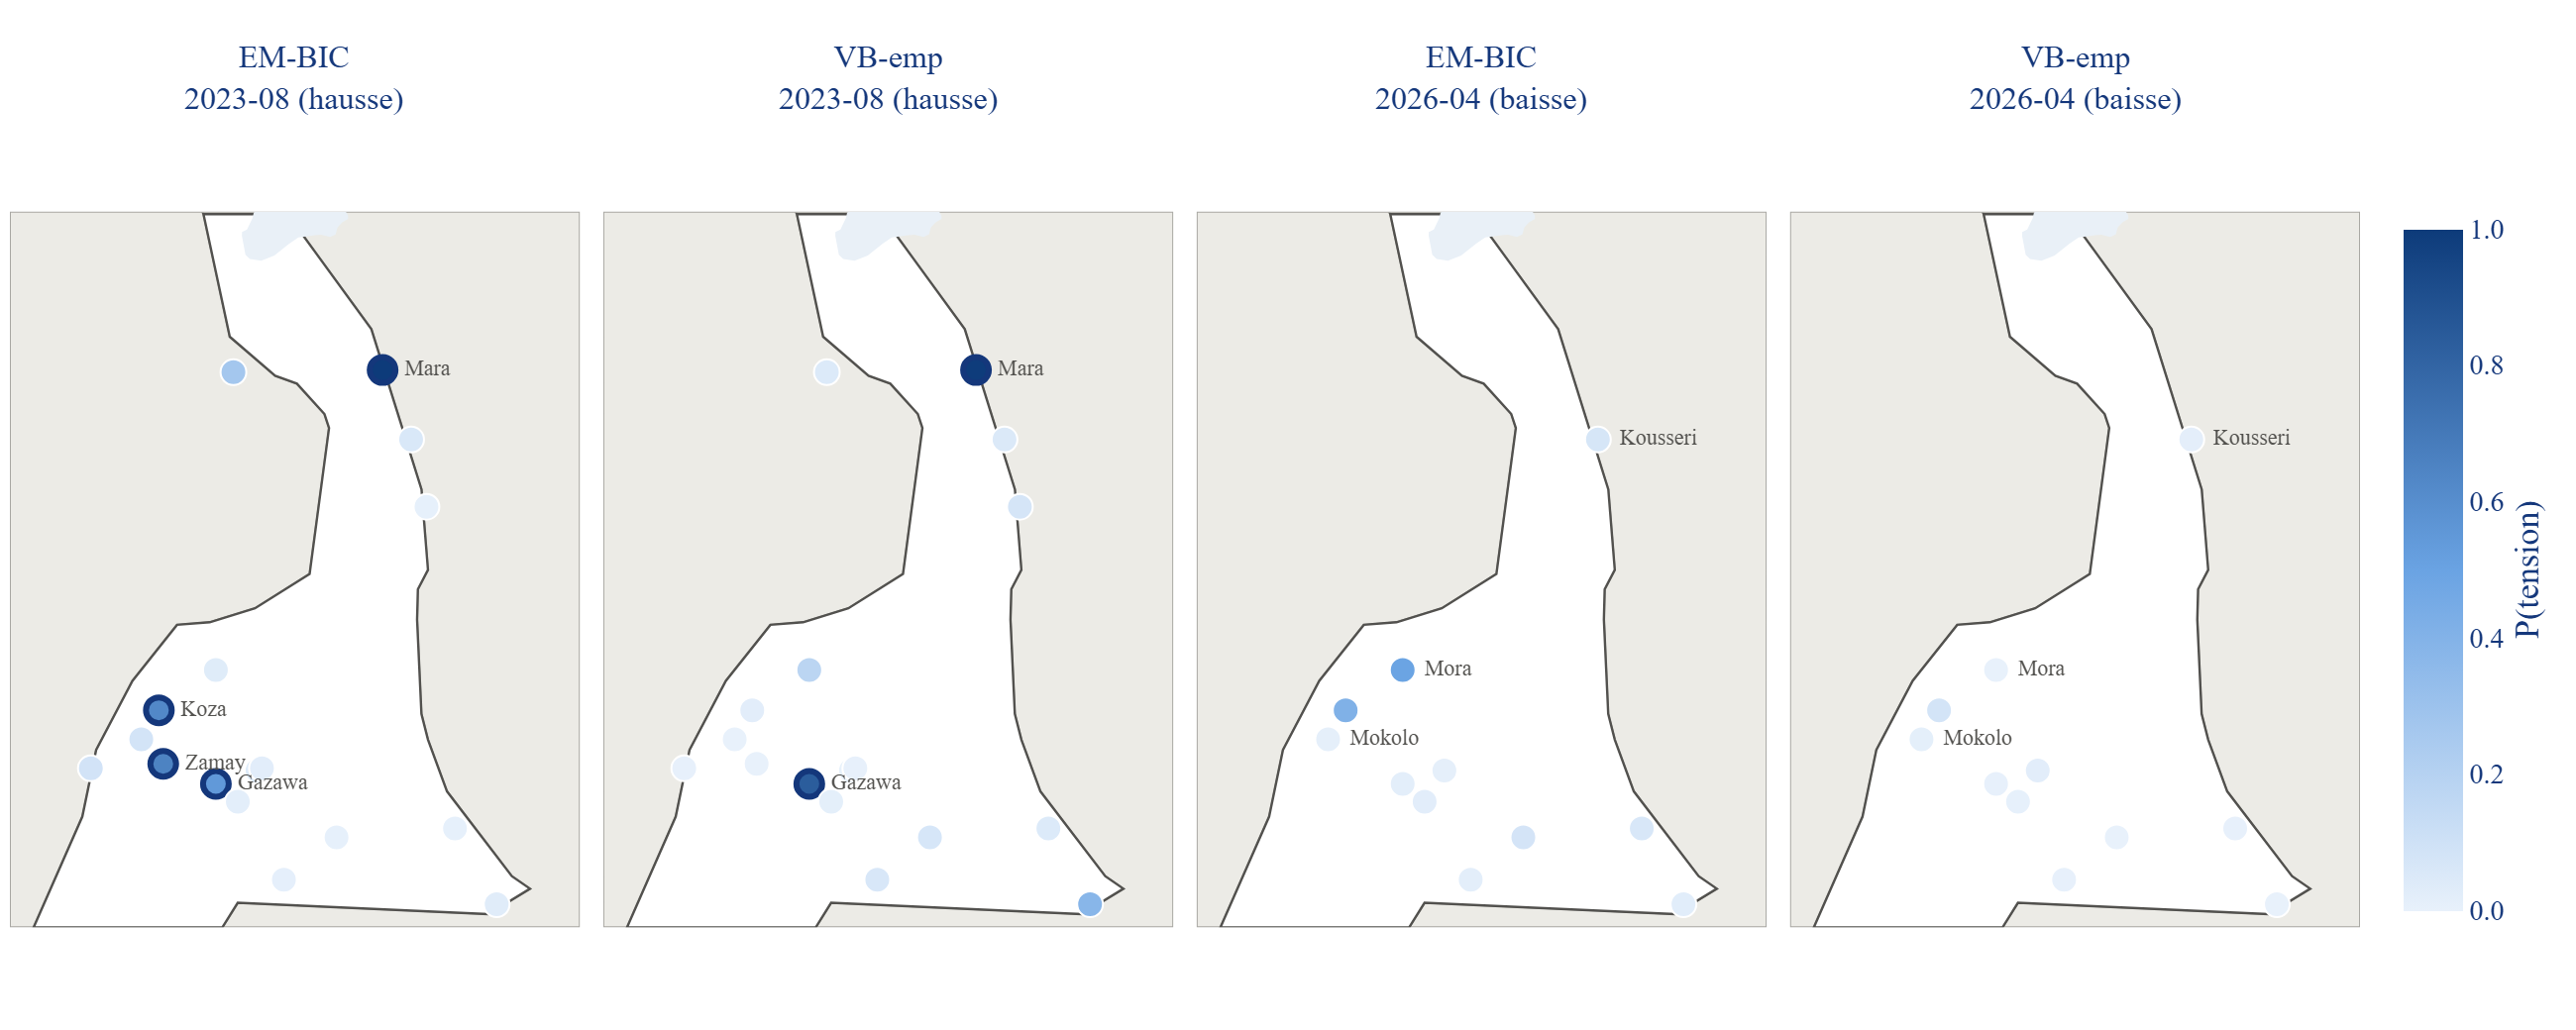
\includegraphics[width=\textwidth]{figures/prix_carte_alerte.png}}{\fbox{\parbox{0.8\textwidth}{\centering figure à générer (\texttt{python run.py --figures})}}}
\caption{Extrême-Nord, mois des deux épisodes datés : probabilité du régime de tension de chaque marché observé selon EM-BIC et le VB à priors empiriques. Contour épais et nom : alerte ($P > 0{,}5$) ; sont aussi nommés les marchés cités par le bulletin de 2026. La hausse d'août 2023~\cite{pam2023bulletin} devrait allumer le régime de tension, la baisse d'avril 2026~\cite{fewsnet2026} ne le devrait pas.}
\label{fig:prix_carte_alerte}
\end{figure}
\tableauGenere{prix_episodes}

\textbf{Synthèse du cas.} La lecture détaillée de chaque décision est archivée dans le dépôt du mémoire (annexe A). Sur toute la période d'apprentissage, l'EM-BIC retient deux régimes, le VB à priors empiriques quatre et le VB calibré huit (tableau~\ref{tab:prix_complet}). Sur le jeu semi-synthétique tiré du modèle EM-BIC, le VB s'écarte davantage du $K$ générateur que l'EM-BIC (écart moyen de 0,35 à 1,02 composante selon $N$), et sa log-vraisemblance de test est inférieure de 0,16 nat par observation, intervalle compris, au-delà de la marge (HP2-LL) : l'équivalence n'est démontrée ni pour $\hat K$ ni pour la vraisemblance, ce qui peut tenir en partie au choix du modèle générateur (section~\ref{sec:validite}). Le nombre de composantes du VB varie bien plus entre configurations de priors plausibles que celui de l'EM entre ses propres choix (HP5, écart de 3,2). Les intervalles de crédibilité du VB couvrent la valeur vraie dans 22 \% des cas pour les poids et 64 \% pour les moyennes, contre 44 \% et 78 \% pour le bootstrap d'EM-BIC : tous sont sous le niveau nominal de 90 \%, mais ceux du VB le sont davantage (écart de 21,5 points pour les poids et de 14,6 points pour les moyennes, tableau~\ref{tab:decisions_prix}), ce que prédit la sous-estimation de variance du champ moyen. Le MAP-EM, qui porte les priors du VB sans loi sur les paramètres, réduit lui aussi les ajustements dégénérés à $N = 60$ et $N = 120$ (HP7), alors que le VB ne le fait de façon démontrée qu'à $N = 120$ (HP3) : l'effet régularisant tient aux priors. Le pipeline EM-BIC coûte 2,6 à 5,0 fois le temps d'un VB pour $N \geq 60$ ; à $N = 30$, l'intervalle du rapport contient 1. Aucune des six comparaisons de prévision ne montre de différence de log-score sur les 32 mois de test : ni le VB, ni l'EM-BIC, ni le mélange en général ne prévoient mieux qu'une loi gaussienne simple sur cette période. Pour l'alerte, les deux méthodes classent de la même façon 83,8 \% des observations, et l'intervalle à 90 \% de la probabilité d'alerte a une largeur moyenne comparable : 0,075 à 0,093 pour le VB, 0,087 à 0,124 pour le bootstrap d'EM-BIC ; il contient le seuil de 0,5 dans 6 à 11 \% des observations selon la méthode et la période (tableau~\ref{tab:prix_alerte}). Au vu des couvertures mesurées, aucun des deux intervalles ne se lit comme une incertitude calibrée.

La confrontation des alertes aux épisodes datés par les bulletins du PAM et de FEWS NET se lit au tableau~\ref{tab:prix_episodes} et aux figures~\ref{fig:prix_alerte}, \ref{fig:prix_carte_alerte} et~\ref{fig:prix_alerte_mois}. En août 2023, mois de la hausse du maïs dans l'Extrême-Nord, l'EM-BIC met en alerte 4 des 17 marchés observés de la région et le VB 2, pour des parts habituelles de 10,3 \% et 12,4 \% des observations de la région. En avril 2026, mois de baisse qui sert de contrôle négatif, aucune des deux méthodes ne met en alerte un des 11 marchés observés, ni les trois marchés cités par FEWS NET. Les deux méthodes ne définissent pas la tension de la même façon : le régime de tension de l'EM-BIC porte surtout sur le maïs (écart moyen $+0{,}11$), celui du VB surtout sur le niébé ($+0{,}15$). Cette confrontation est qualitative et ne constitue pas une validation statistique.

\textbf{Limites. }Outre les limites générales du cas (section~\ref{sec:validite} : trois régions au test, dépendance des observations, régimes sans vérité terrain), trois points lui sont propres. (1) \emph{Changement de distribution} : l'écart moyen du maïs passe de $+0{,}04$ à l'apprentissage à $-0{,}12$ au test (tableau~\ref{tab:prix_descriptif}), conformément à la baisse des céréales signalée par FEWS NET ; les log-scores de test mesurent aussi ce changement. Le modèle de Markov caché, qui modéliserait la persistance des régimes, n'est pas utilisé : le noyau du code ne traite que des émissions scalaires et les séries sont trouées. (2) \emph{Prix nominaux} : l'écart au niveau des douze derniers mois retire la dérive lente, mais pas un choc d'inflation générale. (3) \emph{Accès à la nourriture} : FEWS NET souligne qu'en 2026 des prix bas ne signifient pas une amélioration de l'accès dans les zones de conflit ; l'indicateur décrit les prix, non l'insécurité alimentaire elle-même.


\section{Comparaison pLSA contre LDA}\label{sec:res_texte}
Le corpus et le protocole sont décrits à la section~\ref{sec:texte_methodo}.

\tableauGenere{texte_resume}
\tableauGenere{decisions_texte}

\textbf{Synthèse.} Le pLSA surapprend plus que la LDA aux trois effectifs (HT1, p de Holm 0,006 pour chacun), et l'écart se réduit quand $N$ croît : au vocabulaire principal, l'écart relatif de perplexité (test sur apprentissage) du pLSA vaut $2{,}39 \times 10^{42}$ à $N = 50$, 12\,881 à $N = 200$ et 0,51 à $N = 1\,000$, contre 1,81, 0,53 et 0,14 pour la LDA (tableau~\ref{tab:texte_resume}). Les valeurs extrêmes du pLSA viennent des mots du test auxquels il donne une probabilité nulle (10,8 \% des mots à $N = 50$) ; la moyenne des différences n'est donc pas interprétable, et la décision repose sur les rangs (test de Wilcoxon) et sur l'estimateur de Hodges-Lehmann. À $N = 1\,000$, les deux modèles ont une cohérence (NPMI 0,138 et 0,141) et une pureté (0,607 et 0,617) voisines ; une exécution pLSA sur dix n'y a pas convergé. Deux réserves s'appliquent à cette lecture. D'abord, la LDA du code lisse $\beta$ (pseudo-compte calibré) et le pLSA ne le fait pas : une partie de l'écart aux petits effectifs peut venir des probabilités nulles du pLSA (colonne « Mots nuls ») et non seulement du prior sur $\theta_d$. Ensuite, les exécutions non convergées au plafond d'étapes M sont signalées, et les résultats dépendent du prétraitement et du nombre de thèmes ($K=4$, égal au nombre de groupes).

\section{Analyse et interprétation : bilan des hypothèses de recherche}\label{sec:bilan}
\tableauGenere{bilan_recherche}
\lectureGeneree{recherche}

Le verdict de chaque décision suit la règle déclarée à la section~\ref{sec:decision} (conforme, contraire, non tranché). La lecture d'ensemble ne désigne pas un meilleur algorithme : elle décrit des déplacements. Le VB transfère la sélection de $K$ vers le choix de $K_{\max}$, des hyperparamètres et du seuil d'activité ; il fournit une incertitude approchée dont la couverture est mesurée ; il coûte plus par ajustement que l'EM, ce qui n'établit pas un coût plus élevé que le pipeline EM-BIC en temps total. Les décisions d'équivalence (RH1) indiquent dans quelles conditions les deux algorithmes sont de qualité comparable. La comparaison à $K = 6$ imposé est défavorable à l'EM par construction et ne sert que d'illustration du mécanisme d'élagage.

Les décisions d'équivalence dépendent de la marge fixée a priori ; le tableau~\ref{tab:sensibilite_marges} (annexe H) les rapporte aussi à la moitié et au double de cette marge, la correction de Holm étant recalculée pour chaque variante. Une équivalence qui ne tient qu'à la marge fixée se lit comme fragile.


Le tableau~\ref{tab:2_17} remplace les anciennes listes d'avantages et d'inconvénients par une grille « axe $\times$ preuve » : chaque ligne renvoie à une expérience, à un théorème, ou porte la mention « non testé ».

\tableauGenere{grille_axe_preuve}
Le choix entre les deux algorithmes est donc un arbitrage qui dépend du contexte d'application, précisé par les recommandations de la section~\ref{sec:recommandations}, et non un classement entre une méthode meilleure et une méthode moins bonne.

\subsection{Mise en relation avec la littérature}\label{sec:res_litterature}
Chaque hypothèse de recherche répond à une limite de la littérature (section~\ref{sec:ea_limites}) ; ses décisions se lisent donc face aux sources correspondantes.
\textbf{RH2 et le seuil $d/2$.} Rousseau et Mengersen~\cite{rousseau2011} montrent que, pour le posterior exact, les composantes excédentaires se vident quand $\alpha_0 < d/2$. Le champ moyen reproduit l'ordre des seuils entre formes de covariance (S8), mais ses transitions se situent au-dessus de ces seuils : le résultat nuance la transposition de la théorie au VB sans la contredire, la théorie ne portant pas sur le champ moyen. Le poids de $\alpha_0$ dans la variance du nombre de composantes (69 \%, S9) et la variance de $\hat K$ entre priors plausibles (HP5) confirment que le VB déplace la sélection de $K$ vers ses hyperparamètres.

\textbf{RH3 et la variance du champ moyen.} Les couvertures du VB (22 \% pour les poids, 64 \% pour les moyennes, pour un niveau nominal de 90 \%) confirment la sous-estimation de variance décrite par Wang et Titterington~\cite{wang2005} et par Blei et al.~\cite{blei2017}, et la quantifient sur un jeu réaliste. Elles apportent une nuance : le bootstrap d'EM-BIC reste lui aussi sous le niveau nominal (44 \% et 78 \%), et il l'est encore à $K$ connu (bootstrap d'EM-K : 48 \% et 82 \%) ; la sous-couverture des poids ne tient donc pas seulement à l'incertitude du choix de $K$, que ce bootstrap ne propage pas, et la couverture mesurée est inconditionnelle. Le bootstrap n'est donc pas une référence calibrée dans ce cadre, seulement une référence moins mal calibrée.

\textbf{RH1 et RH4 face aux avantages pratiques du VB.} Bishop~\cite{bishop2006} et Corduneanu et Bishop~\cite{corduneanu2001} présentent l'élagage et l'absence de singularités comme des avantages du VB. Les résultats les confirment en partie : le VB produit moins d'ajustements dégénérés que l'EM à $K_{\max}$ (S6) et fait mieux que l'EM-BIC quand les groupes se chevauchent ou que la dimension croît. Ils les nuancent sur deux points : le MAP-EM obtient la même réduction des ajustements dégénérés (HP7), ce qui attribue l'effet aux priors plutôt qu'à l'inférence variationnelle ; et sur les données de prix, le VB ne retrouve pas mieux le nombre de régimes et prévoit moins bien hors échantillon que l'EM-BIC (HP1, HP2).

\textbf{RH5 et le coût.} L'analyse de complexité (section~\ref{sec:complexite_computationnelle}) prévoit un VB plus coûteux par itération ; la mesure le confirme (1,1 à 2,2 fois). Elle montre aussi que ce surcoût est plus que compensé, en temps total, par le balayage de $K$ de l'EM-BIC, 2,6 à 5,0 fois plus long dès 60 observations (HP4).

\textbf{HT1 et la motivation de la LDA.} Blei, Ng et Jordan~\cite{blei2003} motivent la LDA par le surapprentissage du pLSA, dont le nombre de paramètres croît avec le nombre de documents. Le résultat le confirme aux trois effectifs, avec la réserve que l'écart tient en partie au lissage de $\beta$ dans la LDA.

\section{Discussion critique}\label{sec:discussion_critique}
\textbf{Limites des résultats. }Les limites de la méthode sont déclarées à la section~\ref{sec:validite}.
(1) 22 décisions sur 63 restent non tranchées (tableau~\ref{tab:bilan_recherche}), dont 9 équivalences non démontrées : une équivalence non démontrée n'est pas une différence démontrée. (2) Pour HP7-N120, le plafond de 200 réplications donne une puissance simulée de 0,74, sous l'objectif de 0,8 ; cinq hypothèses sans variance pilote (HS1-sep1, HP3-N30, HP3-N60, HP7-N30, HP7-N60) n'ont pas fixé le nombre de réplications de leur famille. (3) Aucune réplication n'a été exclue pour échec numérique : toutes les décisions portent sur 110 réplications (scénarios), 50, 100 ou 200 (prix) et 10 (texte). (4) Le bruit d'optimisation de la log-vraisemblance (0,066 nat par observation, quantile à 95 \% de l'écart entre deux ajustements d'un même bras) dépasse la marge de 0,05 : une équivalence en log-vraisemblance non démontrée peut refléter ce bruit. Pour HP2-LL, l'intervalle $[-0{,}172 ; -0{,}147]$ est toutefois entièrement au-delà de la marge, ce qui établit un écart et non une simple absence d'équivalence. (5) Avec vingt relances, la probabilité d'atteindre le meilleur optimum des 200 relances pilotes est d'au moins 0,99 dans 47 \% des cas pilotes seulement (minimum 0,10), surtout à $K$ surdimensionné ; EM et VB ayant le même nombre de relances, aucun bras n'en est avantagé. (6) Le chronométrage a été interrompu une fois par une reprise de l'instance de calcul ; chaque répétition étant mémorisée, seules les répétitions en cours ont été refaites.

\textbf{Précautions d'interprétation. }Outre les limites de la méthode (section~\ref{sec:validite} : dimension au plus 20, jeu semi-synthétique tiré d'EM-BIC, période de test du cas pratique, régimes sans vérité terrain), deux précautions portent sur la lecture des résultats. (1) Une équivalence n'est démontrée qu'à la marge fixée (0,05 pour l'ARI et pour la log-vraisemblance par observation) ; la sensibilité à la moitié et au double de la marge en donne la portée. (2) Le VB étudié est le champ moyen conjugué ; ses conclusions ne s'étendent pas aux familles variationnelles plus riches (section~\ref{sec:variantes_vb}).

\textbf{Reprises suggérées par les résultats. }Les perspectives générales sont rassemblées dans la conclusion ; les résultats en suggèrent trois plus précises. Pour S3 à $K = 4$ et 5 et pour HP1 à $N = 30$, 120 et 500, l'équivalence n'est démontrée qu'au double de la marge : l'écart y est de l'ordre de la marge elle-même, et seule une marge justifiée par un usage précis permettrait de conclure. L'écart de log-vraisemblance entre VB et EM-BIC sur les prix (HP2) mérite d'être reproduit avec un jeu semi-synthétique tiré d'un autre modèle que l'EM-BIC, pour séparer l'effet de la méthode de celui du générateur. Enfin, la sous-couverture des deux méthodes appelle une comparaison à une référence calibrée (posterior par MCMC) et à un bootstrap qui propage le choix de $K$.

\section{Recommandations pratiques}\label{sec:recommandations}
Cette section traduit les résultats en un guide de choix entre EM classique et EM variationnel pour une situation pratique.

\tableauGenere{guide_decision}
Ce guide ne recommande pas un algorithme dans l'absolu : chaque ligne indique le niveau de preuve disponible. Il est complété par trois bonnes pratiques indépendantes de l'algorithme. Premièrement, standardiser les données avant l'ajustement, les deux algorithmes étant sensibles à l'échelle relative des dimensions ; Iris, laissé en centimètres avec une régularisation absolue commune à tous les jeux, en montre l'effet (section~\ref{sec:iris_methodo}). Deuxièmement, multiplier les initialisations (\texttt{n\_init} > 1) pour l'EM comme pour le VB. Troisièmement, utiliser un critère d'arrêt commun lorsque l'on compare des nombres d'itérations ou des temps, et rapporter les exécutions non convergées.

\section{Synthèse du chapitre}\label{sec:conclusion_du_chapitre_3}
\enlargethispage{2\baselineskip}%
Ce chapitre a présenté les résultats dans l'ordre de la preuve : illustrations exploratoires du mécanisme d'élagage, scénarios confirmatoires répliqués, cas pratique sur un problème réel du Cameroun et comparaison pLSA contre LDA. Le bilan des hypothèses de recherche (tableau~\ref{tab:bilan_recherche}) et la grille « axe $\times$ preuve » (tableau~\ref{tab:2_17}) rattachent chaque conclusion à une décision lue dans un fichier de résultats, à un théorème ou à la mention « non testé ». Sur 63 décisions, 31 sont conformes aux hypothèses, 4 contraires (toutes sur la couverture du bootstrap, que l'hypothèse supposait proche du niveau nominal), 22 non tranchées et 6 sont des différences sans sens prédit. Les conditions de validité de ces conclusions sont celles de la section~\ref{sec:validite} : l'élagage dépend des priors, de $K_{\max}$ et du seuil d'activité ; les variantes de covariance non pleines utilisent un critère approché ; le cas des prix repose sur une période de test qui diffère de l'apprentissage et sur des régimes reliés à la réalité par une confrontation qualitative aux bulletins d'alerte.

\chapter*{Conclusion générale}
\addcontentsline{toc}{chapter}{Conclusion générale}
\markboth{CONCLUSION GÉNÉRALE}{CONCLUSION GÉNÉRALE}
Ce mémoire a comparé l'EM classique et l'EM variationnel pour les modèles de mélange, sur trois niveaux d'inférence, en reliant chaque avantage et chaque inconvénient à un théorème, à une expérience ou à la mention « non testé ».

\section*{Réponses aux hypothèses de recherche}
\addcontentsline{toc}{section}{Réponses aux hypothèses de recherche}
Les 63 décisions déclarées donnent le bilan suivant (tableau~\ref{tab:bilan_recherche}). \textbf{RH1} : aucune supériorité générale n'est démontrée. Le VB et l'EM-BIC sont équivalents quand les groupes sont séparés ou contaminés par des aberrations ; le VB fait mieux quand les groupes se chevauchent ou que la dimension croît ; sur les prix, il retrouve moins bien le nombre de régimes et prévoit moins bien hors échantillon, et aucune méthode ne prévoit mieux qu'une loi gaussienne simple. \textbf{RH2} : le nombre de composantes du VB dépend surtout de $\alpha_0$ (69 \% de la variance) et varie davantage entre priors plausibles que celui de l'EM entre ses propres choix. \textbf{RH3} : les intervalles du VB couvrent bien moins que le niveau nominal (22 \% et 64 \% pour 90 \%), et moins que le bootstrap d'EM-BIC (44 \% et 78 \%), lui-même sous ce niveau. \textbf{RH4} : le VB produit moins d'ajustements dégénérés que l'EM de même capacité, et le MAP-EM aussi, ce qui attribue l'effet aux priors ; la LDA surapprend moins que le pLSA. \textbf{RH5} : un ajustement VB coûte 1,1 à 2,2 fois plus par itération, mais le pipeline EM-BIC coûte 2,6 à 5 fois plus en temps total dès 60 observations. La thèse défendue en introduction en sort précisée : le VB ne bat pas l'EM, il déplace la sélection de $K$ vers ses hyperparamètres, régularise par ses priors (comme le ferait un MAP-EM) et donne des intervalles qu'il ne faut pas lire comme calibrés ; chaque terme de ce constat renvoie à une ligne de la grille du tableau~\ref{tab:2_17}.

\section*{Synthèse des contributions}
\addcontentsline{toc}{section}{Synthèse des contributions}
Ce travail apporte les éléments suivants, sans prétention de nouveauté théorique :

\begin{itemize}
\item une présentation unifiée des fondements communs (inégalité de Jensen, ELBO, divergence de Kullback-Leibler) distinguant trois niveaux d'inférence, avec une redémonstration de l'équivalence de Neal et Hinton~\cite{neal1998} par passage à la limite (section~\ref{sec:de_l_energie_libre_de}) ;
\item un comparateur MAP-EM, qui isole l'effet du prior de celui de l'inférence bayésienne complète ;
\item un protocole de comparaison à critère d'arrêt commun, avec baseline EM-BIC et EM-ICL, tests appariés, tests d'équivalence et correction de Holm, appliqué à dix scénarios synthétiques (S1 à S10) et à un jeu semi-synthétique ;
\item un cas pratique sur un problème réel du Cameroun, l'alerte sur les prix des denrées de base (données publiques du PAM, 2021-2026~\cite{pam2026donnees}), avec hypothèses déclarées avant tout ajustement, validation temporelle, probabilité d'alerte munie d'un intervalle et comparaisons de prévision par le test de Diebold--Mariano, ainsi qu'une comparaison pLSA contre LDA ;
\item une implémentation en PyTorch testée et archivée, qui régénère chaque tableau.
\end{itemize}

\section*{Limites du travail}
\addcontentsline{toc}{section}{Limites du travail}
Les limites de la méthode et des résultats sont détaillées aux sections~\ref{sec:validite} et~\ref{sec:discussion_critique} ; trois d'entre elles bornent la portée des conclusions. (1) Certains résultats sont des constats, non des démonstrations : le critère des variantes tied, diag et sphérique du VB est une approximation faute d'ELBO dérivée, et le transfert du seuil $d/2$ du posterior exact au champ moyen est testé, non démontré ; l'irréversibilité de l'élagage, la dépendance à $K_{\max}$ et la consistance restent « non testées » ou partiellement testées. (2) Le cas des prix repose sur des choix de variables et un seuil d'alerte de 0,5 posés sans alternative testée (annexe E), sans réestimation en fenêtre glissante ; la comparaison pLSA contre LDA porte sur un corpus de quatre groupes, avec une LDA à $\beta$ ponctuel et non un VB complet. (3) Les temps de calcul dépendent d'une machine et d'une implémentation (annexe D), et la vision, la bio-informatique et la recommandation ne sont pas testées.

\section*{Perspectives}
\addcontentsline{toc}{section}{Perspectives}
Sur le plan expérimental : étendre la comparaison à la grande dimension avec des covariances structurées, éprouver l'irréversibilité de l'élagage par des initialisations adverses, réestimer les modèles de prix en fenêtre glissante et modéliser la persistance des régimes par un modèle de Markov caché tolérant les mois manquants. Sur le plan méthodologique : un critère d'élagage indépendant du seuil d'activité, l'ELBO des variantes de covariance, des familles variationnelles plus riches (flux normalisants) ou d'autres divergences que la KL inverse, et une confrontation des seuils de type $d/2$ à un posterior approché par MCMC. Sur le plan applicatif : tester le cas des prix sur les autres pays de la CEMAC et du bassin du lac Tchad couverts par la base du PAM, et confronter les alertes aux phases du Cadre Harmonisé avec les analystes de la sécurité alimentaire.

%% ==== Bibliographie ====
\printbibliography[title={Bibliographie}, heading=bibintoc]
\markboth{BIBLIOGRAPHIE}{BIBLIOGRAPHIE}


%% ==== Annexes ====
\chapter*{Annexes}
\addcontentsline{toc}{chapter}{Annexes}
\markboth{ANNEXES}{ANNEXES}
\section*{Annexe A : Code source}
\addcontentsline{toc}{section}{Annexe A : Code source}
Les résultats de ce mémoire sont produits par les modules Python suivants, rangés dans le paquet \texttt{emvb/} : \texttt{algorithmes.py} (EM classique, MAP-EM, EM variationnel, ELBO, variantes, Baum-Welch, LDA, pLSA, métriques), \texttt{risque.py} (loi prédictive du VB, test de Diebold--Mariano), \texttt{statistique.py} (Wilcoxon exact, TOST, Holm, bootstrap), \texttt{comparaison.py} (protocole des bras, statistiques de comparaison), \texttt{hypotheses.py} (hypothèses déclarées), \texttt{parametres.py} et \texttt{calibrage.py} (registre et calibrage des paramètres), \texttt{scenarios.py} (scénarios synthétiques S1 à S10), \texttt{etape\_validation.py}, \texttt{etape\_illustrations.py} et \texttt{etape\_chronometrage.py} (validations du chapitre~\ref{chap:fondements} et expériences du chapitre~\ref{chap:methodologie}), \texttt{donnees.py} et \texttt{etape\_prix.py} (cas pratique des prix alimentaires), \texttt{etape\_texte.py} (comparaison pLSA contre LDA), \texttt{figures.py} et \texttt{tex\_tables.py} (figures et tableaux \LaTeX{} produits depuis les résultats), enfin \texttt{run.py}, \texttt{persistance.py} et \texttt{superviseur.py} (orchestration reprenable après interruption). Le dépôt complet, avec son jeu de tests (\texttt{tests/}), est publié sur GitHub (section A.1) ; l'étiquette Git et le DOI Zenodo de la version définitive restent à créer au moment de l'archivage. Le tableau suivant indique, pour chaque fonction de la bibliothèque, la section et l'équation correspondantes.

\begin{table}[H]
\centering
\small
\setlength{\tabcolsep}{0.14cm}
\begin{tabular}{|p{5.2cm}|p{4.4cm}|p{5.2cm}|}
\hline
\textbf{Fonction} & \textbf{Section} & \textbf{Équations} \\
\hline
em\_classique & \ref{sec:em_classique} & (\ref{eq:1_15}), (\ref{eq:1_16}), (\ref{eq:1_18}) \\
\hline
em\_stochastique, em\_online & \ref{sec:variantes_em} & Celeux et Diebolt, Cappé et Moulines \\
\hline
em\_variationnel & \ref{sec:em_variationnel} & (\ref{eq:1_26}) à (\ref{eq:1_30}) \\
\hline
elbo\_gmm\_bayesien & \ref{sec:calcul_elbo} & (\ref{eq:1_31}) \\
\hline
svi\_gmm & \ref{sec:variantes_vb} & Hoffman et al. \\
\hline
lda\_variationnel, plsa\_em & \ref{sec:texte_methodo} & Blei, Ng et Jordan~\cite{blei2003} ; Hofmann~\cite{hofmann1999} \\
\hline
bic, aic & \ref{sec:selection_modele} & (\ref{eq:2_4}), (\ref{eq:2_5}) \\
\hline
\end{tabular}
\caption{Correspondance entre fonctions du code, sections et équations}
\end{table}

\subsection*{A.1 Accès au code complet}
Le code complet (environ 1\,400 lignes pour \texttt{algorithmes.py}, 250 pour \texttt{risque.py}, plus les scripts d'expériences et les tests) n'est pas reproduit ici. Les modules sont rangés dans le paquet \texttt{emvb/} du dépôt, et \texttt{run.py}, à la racine, lance les étapes. Il est disponible dans le dépôt public \href{\depot}{\texttt{github.com/Kanaicare8/em-classique-vs-variationnel}}. Chaque QR code ci-dessous ouvre le fichier correspondant sur la branche \texttt{main}.

\begin{center}
\begin{minipage}[t]{0.31\linewidth}\centering
\qrcode[height=2.4cm]{\depot}\\[0.3em]
{\footnotesize\textbf{Dépôt complet}}\\
{\scriptsize\texttt{em-classique-vs-variationnel}}
\end{minipage}\hfill
\qrfichier{emvb/algorithmes.py}{Algorithmes}\hfill
\qrfichier{emvb/risque.py}{Gestion du risque}\\[1.2em]
\qrfichier{emvb/comparaison.py}{Protocole « 5 EM + VB »}\hfill
\qrfichier{emvb/scenarios.py}{Scénarios S1 à S10}\hfill
\qrfichier{run.py}{Lancement des étapes}
\end{center}

\subsection*{A.2 Extraits commentés}
Les trois extraits suivants sont copiés sans modification du code exécuté. Ils montrent la traduction directe des équations en calcul tensoriel : toutes les relances (dimension \texttt{B}) sont traitées en un seul lot, et les responsabilités sont normalisées en log-espace (équation~\ref{eq:1_18}).

\textbf{Étape E de l'EM classique} (\texttt{algorithmes.py}, équation~\ref{eq:1_15}).
\begin{lstlisting}[language=Python]
def _etape_e_lot(dp: "_Prep", pi: Tensor, mu: Tensor, cov: Tensor):
    """Étape E (1.15) en log-espace pour toutes les relances : (r (B,N,K), log p(x_n | theta) (B,N), ok (B,))."""
    B, K, D = mu.shape
    N = dp.N
    r = dp.X.new_empty(B, N, K)
    ln = dp.X.new_empty(B, N)
    ok = torch.empty(B, dtype=torch.bool)
    for sl in _tranches(B, K, N):
        lp, ok[sl] = _log_gauss_lot(dp, mu[sl], cov[sl])
        log_r = (torch.log(pi[sl] + 1e-300)[:, :, None] + lp).transpose(1, 2)    # (b,N,K)
        ln[sl] = torch.logsumexp(log_r, dim=2)
        r[sl] = torch.exp(log_r - ln[sl][..., None])
    return r, ln, ok
\end{lstlisting}

\textbf{Étape E de l'EM variationnel} (\texttt{algorithmes.py}, équations~\ref{eq:1_27} et \ref{eq:1_30}). Le terme $\mathbb{E}[\log \pi_k] = \psi(\alpha_k) - \psi(\sum_j \alpha_j)$ porte le mécanisme d'élagage de la section~\ref{sec:elagage}.
\begin{lstlisting}[language=Python]
def _etape_e_var_lot(dp, P):
    """Étape E variationnelle, équation (1.27), avec la forme quadratique (1.30), en lot : (r (B,N,K), log_norm (B,N))."""
    N, D = dp.N, dp.D
    B, K = P["alpha"].shape
    Elogpi = torch.special.digamma(P["alpha"]) - torch.special.digamma(P["alpha"].sum(-1, keepdim=True))
    Elogdet, Elam = _attendus_lot(P, D)
    r = dp.X.new_empty(B, N, K)
    ln = dp.X.new_empty(B, N)
    for sl in _tranches(B, K, N):
        quad = D / P["beta"][sl][..., None] + _forme_quadratique(dp, Elam[sl], P["m"][sl])
        log_rho = (Elogpi[sl][..., None] + 0.5 * Elogdet[sl][..., None] - 0.5 * D * LOG2PI - 0.5 * quad).transpose(1, 2)
        ln[sl] = torch.logsumexp(log_rho, dim=2)
        r[sl] = torch.exp(log_rho - ln[sl][..., None])
    return r, ln
\end{lstlisting}

\textbf{Variable du cas pratique} (\texttt{donnees.py}, écart causal du log-prix à son niveau des douze mois précédents, section~\ref{sec:prix_methodo}).
\begin{lstlisting}[language=Python]
def ecart(m, c, t):
    s = serie.get((m, c), {})
    if t not in s:
        return None
    passe = [s[u] for u in range(t - fenetre, t) if u in s]
    return s[t] - sum(passe) / len(passe) if len(passe) >= releves_min else None
\end{lstlisting}
Seuls les relevés antérieurs au mois $t$ entrent dans le niveau de référence ; un test unitaire recalcule une observation à la main pour le vérifier.

\subsection*{A.3 Expériences et cas pratique}
L'orchestrateur \texttt{run.py} enchaîne les étapes (calibrage, validation, illustrations, chronométrage, scénarios, prix, texte) ; chaque étape est une liste d'unités indépendantes, exécutées en parallèle et écrites atomiquement dans un magasin d'artefacts, de sorte qu'un calcul interrompu (erreur, coupure de courant, arrêt volontaire) reprend exactement où il s'était arrêté lorsqu'on relance la même commande ; \texttt{superviseur.py} relance automatiquement le calcul après un arrêt non voulu. L'option \texttt{--rapide} exécute une version réduite dans un magasin séparé. Les tableaux (\texttt{python -m emvb.tex\_tables}) et les figures (\texttt{python run.py --figures}) sont produits depuis le magasin, sans recalcul ; aucun nombre des tableaux n'est saisi à la main.

\subsection*{A.4 Corpus et résultats de la comparaison pLSA contre LDA}
Le corpus (sous-ensemble de 20 Newsgroups) est lu et prétraité par \texttt{donnees.py} (section~\ref{sec:texte_methodo}) ; les ajustements pLSA et LDA sont faits par \texttt{etape\_texte.py}, une unité par taille de vocabulaire, par taille $N$ et par réplication, écrite dans le magasin de l'étape \texttt{texte}, d'où les tableaux de la section~\ref{sec:res_texte} sont produits.


\section*{Annexe B : Détail du calcul de l'ELBO pour le GMM bayésien}
\addcontentsline{toc}{section}{Annexe B : Détail du calcul de l'ELBO pour le GMM bayésien}
Cette annexe donne l'implémentation, en PyTorch, du calcul exact de l'ELBO de l'équation~\eqref{eq:1_31}~\cite[éq.~10.70 à 10.77]{bishop2006}. Les sept termes sont : $\mathbb{E}[\log p(X|Z,\mu ,\Lambda )]$, $\mathbb{E}[\log p(Z|\pi )]$, $\mathbb{E}[\log p(\pi )]$ et $\mathbb{E}[\log p(\mu ,\Lambda )]$ (partie vraisemblance et priors), puis $-\mathbb{E}[\log q(Z)]$, $-\mathbb{E}[\log q(\pi )]$ et $-\mathbb{E}[\log q(\mu ,\Lambda )]$ (entropies des facteurs variationnels). La fonction \texttt{\_ln\_B} calcule la constante de normalisation de la loi de Wishart ; \texttt{\_attendus} calcule $\mathbb{E}[\log |\Lambda _{k}|]$ (équation~\ref{eq:1_29}).

\begin{lstlisting}[language=Python]
def _ln_B(W, nu, D):
    """log de la constante de normalisation de la Wishart, ln B(W, nu)."""
    i = torch.arange(1, D + 1, dtype=torch.float64)
    lg = torch.lgamma((nu[..., None] + 1 - i) / 2).sum(-1)
    return -0.5 * nu * torch.logdet(W) - (0.5 * nu * D * LN2 + D * (D - 1) / 4 * LNPI + lg)

def _attendus(P, D):
    """E[ln|Lambda_k|] (1.29) et E[Lambda_k] pour chaque composante."""
    if P["cov_type"] in ("full", "tied"):
        i = torch.arange(1, D + 1, dtype=torch.float64)
        Elogdet = (torch.special.digamma((P["nu"][:, None] + 1 - i) / 2).sum(-1)
                   + D * LN2 + torch.logdet(P["W"]))
        Elam = P["nu"][:, None, None] * P["W"]
    else:
        psi = torch.special.digamma(P["a"]) - torch.log(P["b"])
        Elogdet = psi.sum(-1)
        Elam = torch.diag_embed(P["a"] / P["b"])
    return Elogdet, Elam

def elbo_gmm_bayesien(r, Nk, xbar, Sk, P, pr: PrioriNW):
    """
    ELBO du GMM bayésien (équation 1.31, détail dans Bishop 2006, éq. 10.70 à 10.77).
    Disponible pour la covariance pleine.
    """
    K, D = xbar.shape
    alpha, beta, m, nu, W = P["alpha"], P["beta"], P["m"], P["nu"], P["W"]
    Elogpi = torch.special.digamma(alpha) - torch.special.digamma(alpha.sum())
    Elogdet, _ = _attendus(P, D)
    dm = xbar - m
    t_trace = torch.einsum("kde,ked->k", Sk, W)
    t_quad = torch.einsum("kd,kde,ke->k", dm, W, dm)
    e_x = 0.5 * (Nk * (Elogdet - D / beta - nu * t_trace - nu * t_quad - D * LOG2PI)).sum()
    e_z = (Nk * Elogpi).sum()
    a0 = pr.alpha0
    ln_c0 = math.lgamma(K * a0) - K * math.lgamma(a0)
    e_pi = ln_c0 + (a0 - 1.0) * Elogpi.sum()
    W0 = torch.linalg.inv(pr.W0inv)
    d0 = m - pr.m0
    quad_m = torch.einsum("kd,kde,ke->k", d0, W, d0)
    nu0_t = torch.tensor(pr.nu0)
    lnB0 = _ln_B(W0, nu0_t, D)
    e_muLam = (0.5 * (D * math.log(pr.beta0 / (2 * math.pi)) + Elogdet - D * pr.beta0 / beta
                      - pr.beta0 * nu * quad_m).sum()
               + K * lnB0 + 0.5 * (pr.nu0 - D - 1) * Elogdet.sum()
               - 0.5 * (nu * torch.einsum("de,ked->k", pr.W0inv, W)).sum())
    q_z = torch.xlogy(r, r).sum()
    ln_c = torch.lgamma(alpha.sum()) - torch.lgamma(alpha).sum()
    q_pi = ((alpha - 1.0) * Elogpi).sum() + ln_c
    H = -_ln_B(W, nu, D) - 0.5 * (nu - D - 1) * Elogdet + 0.5 * nu * D
    q_muLam = (0.5 * Elogdet + 0.5 * D * torch.log(beta / (2 * math.pi)) - 0.5 * D - H).sum()
    return float(e_x + e_z + e_pi + e_muLam - q_z - q_pi - q_muLam)
\end{lstlisting}
\begin{center}\small\emph{Extrait de code : calcul de l'ELBO du GMM bayésien (équation~\ref{eq:1_31})}\end{center}

\section*{Annexe C : Table de correspondance des symboles mathématiques}
\addcontentsline{toc}{section}{Annexe C : Table de correspondance des symboles mathématiques}
Le tableau ci-dessous rappelle la signification des principaux symboles mathématiques employés dans ce mémoire, à des fins de référence rapide.

\begin{table}[H]
\centering
\small
\setlength{\tabcolsep}{0.14cm}
\begin{tabular}{|p{7.42cm}|p{7.42cm}|}
\hline
\textbf{Symbole} & \textbf{Signification} \\
\hline
X = \{$x_{1}$,\ldots{},$x_{N}$\} & Observations (données) \\
\hline
Z = \{$z_{1}$,\ldots{},$z_{N}$\} & Variables latentes \\
\hline
$\theta $ & Paramètres du modèle \\
\hline
K & Nombre de composantes du mélange \\
\hline
$\pi _{k}$ & Poids de la composante k \\
\hline
$\mu _{k}$, $\Sigma _{k}$ & Moyenne et covariance de la composante k \\
\hline
$r_{ik}$ & Responsabilité de la composante k pour l'observation i \\
\hline
$\ell $($\theta $) & Log-vraisemblance incomplète \\
\hline
Q($\theta $|$\theta ^{t}$) & Espérance de la log-vraisemblance complète \\
\hline
ELBO(q,$\theta $) & Borne inférieure de l'évidence \\
\hline
KL[$q\Vert p$] & Divergence de Kullback-Leibler \\
\hline
q($\theta $,Z) & Distribution variationnelle \\
\hline
$\alpha _{0}$, $m_{0}$, $\beta _{0}$, $W_{0}$, $\nu _{0}$ & Hyperparamètres des priors (Dirichlet, Normal-Wishart) \\
\hline
$\psi $($\cdot $) & Fonction digamma \\
\hline
$N_{k}$ & Nombre effectif de points assignés à la composante k \\
\hline
\end{tabular}
\end{table}
\section*{Annexe D : Environnement logiciel et reproductibilité}
\addcontentsline{toc}{section}{Annexe D : Environnement logiciel et reproductibilité}
Les calculs dont les résultats figurent dans ce mémoire ont été exécutés sur une instance de calcul dans le nuage de 32 cœurs logiques et 61,6 Go de mémoire, louée à l'heure ; la machine personnelle de l'auteur n'a servi qu'à écrire le code et le document. À chaque lancement, \texttt{run.py} enregistre la machine et les logiciels (système, processeur, nombre de cœurs, mémoire, versions de Python et de PyTorch, commit Git du code exécuté, nombre de processus) dans \texttt{resultats/environnement.json} et ajoute une ligne à \texttt{resultats/environnement\_historique.jsonl}. Le tableau suivant est produit depuis ce fichier, sans saisie manuelle ; il regroupe les lancements par configuration.

\tableauGenere{environnement}

Chaque processus de calcul n'utilise qu'un fil d'exécution (\texttt{torch.set\_num\_threads(1)}) ; les unités indépendantes d'une étape sont réparties sur plusieurs processus, et les sous-calculs des unités longues du calibrage sur des processus supplémentaires (variable \texttt{ICARE\_SOUS\_TRAVAILLEURS}). Les temps mesurés pendant ces calculs parallèles le sont sous charge : ils se comparent entre bras d'une même unité, non entre lancements. Le coût des algorithmes (HP4) est mesuré à part, par l'étape de chronométrage lancée seule sur l'instance, dans un seul processus.

Toutes les graines sont dérivées de façon déterministe du rôle de chaque tirage (empreinte SHA-256 du rôle, fonction \texttt{persistance.graine}) : un jeu de données, une réplication, un rééchantillonnage ou un ajustement reçoivent chacun une graine propre, et les réplications pilotes du calibrage des graines disjointes de celles des étapes confirmatoires. Les $n$ relances d'un ajustement utilisent les graines $g, g+1, \dots, g+n-1$, où $g$ est la graine de l'ajustement. En précision double, deux exécutions du même code sur la même machine donnent des résultats identiques, et le calcul parallèle des sous-calculs donne les mêmes valeurs que le calcul séquentiel (vérification bit à bit par \texttt{scripts/verifier\_parallele.py}). Des différences minimes peuvent apparaître avec une autre version de PyTorch ou un autre processeur, en raison de l'ordre des opérations en virgule flottante. Les versions des bibliothèques principales sont fixées dans \texttt{requirements.txt}.

Le protocole est entièrement scripté : \texttt{python run.py} réalise les expériences, écrit les tableaux (fichiers \texttt{.csv}) et les figures (\texttt{.html} interactifs et \texttt{.png}) ; la marche à suivre figure dans \texttt{docs/LANCEMENT.md}.

\section*{Annexe E : Registre des paramètres}
\addcontentsline{toc}{section}{Annexe E : Registre des paramètres}
Le registre complet (chaque paramètre utilisé par le code, avec sa valeur, son statut, sa justification, ses références et l'étude de calibrage qui le fixe, section~\ref{sec:calibrage}) est produit par le code et archivé dans le dépôt du mémoire (annexe A, fichiers \texttt{emvb/parametres.py} et \texttt{resultats/tables/calibrage\_registre.csv}). Le tableau~\ref{tab:registre_resume} en donne les valeurs calibrées principales, lues dans \texttt{resultats/calibrage/}.

\begin{table}[H]
\centering
\small
\begin{tabular}{@{}lll@{}}
\toprule
\textbf{Paramètre} & \textbf{Valeur} & \textbf{Règle (section~\ref{sec:calibrage})} \\
\midrule
Tolérance d'arrêt relative & $10^{-8}$ & accord avec une référence à $10^{-10}$ \\
Plafond d'étapes M & 1\,800 & maximum observé, arrondi à la centaine \\
Itérations de Lloyd (k-means) & 100 & moins de 1 \% des exécutions au plafond \\
Régularisation $\varepsilon$ des covariances & 0,1 & rang moyen hors pli \\
Relances (toutes familles) & 20 & nombre fixe, probabilité rapportée \\
Relances du texte (pLSA ; LDA) & 6 ; 20 & meilleure relance à 0,1 \% près \\
Réplications (scénarios ; prix) & 110 ; 50 à 200 & puissance simulée 0,8 \\
Réplications (texte) & 10 & puissance simulée 0,8 \\
LDA : $\alpha$ ; lissage de $\beta$ & 0,718 ; 0,0665 & divisions successives \\
Bootstrap des intervalles ; tirages de $q$ & 2\,000 ; 8\,000 & erreur Monte Carlo \\
\bottomrule
\end{tabular}
\caption{Valeurs calibrées principales du registre des paramètres}\label{tab:registre_resume}
\end{table}

\subsection*{Décisions du cas pratique}
Le tableau~\ref{tab:registre_decisions_prix} donne, pour chaque décision du cas pratique, ce qui est retenu, les alternatives écartées, la raison du choix et ce qui le vérifie ; « posé » signifie fixé par le protocole sans être mis à l'épreuve.

{\scriptsize
\setlength{\tabcolsep}{3pt}
\begin{longtable}{>{\raggedright\arraybackslash}p{1.9cm}>{\raggedright\arraybackslash}p{2.9cm}>{\raggedright\arraybackslash}p{2.9cm}>{\raggedright\arraybackslash}p{3.9cm}>{\raggedright\arraybackslash}p{3.0cm}}
\caption{Registre des décisions du cas pratique : retenu, alternatives, raison, vérification}\label{tab:registre_decisions_prix}\\
\toprule
\textbf{Décision} & \textbf{Retenu} & \textbf{Alternatives écartées} & \textbf{Raison} & \textbf{Vérification} \\
\midrule
\endfirsthead
\toprule
\textbf{Décision} & \textbf{Retenu} & \textbf{Alternatives écartées} & \textbf{Raison} & \textbf{Vérification} \\
\midrule
\endhead
\bottomrule
\endfoot
Source & base de prix du PAM (HDX) & relevés de terrain, autres bases & publique, mensuelle, licence ouverte, 83 marchés & posé \\
Panier & maïs blanc, riz importé, niébé & autres denrées de la base & couverture des séries ; céréale locale, céréale importée, légumineuse & posé, non testé \\
Prix & détail, XAF/kg & gros, autres unités & prix payé par les ménages, unité commune & posé \\
Variable & écart du log-prix au niveau des 12 mois précédents & écart à une tendance saisonnière (ALPS), variation mensuelle & causale, retire l'inflation et la saisonnalité moyenne, tolère les mois manquants & posé, non testé \\
Fenêtre & 12 mois & 6 ou 24 mois & une année agricole complète & posé, non testé \\
Relevés minimum & 3 & de 1 à 6 & couverture des séries & posé, non testé \\
Nettoyage & pics isolés d'un facteur 3 & aucun, facteur 2 ou 4 & virgule décalée ; plus forte hausse mensuelle citée : 24 \% & posé après inspection (écart au protocole 3) ; 21 relevés listés dans le dépôt du mémoire (annexe A) \\
Observation retenue & les trois écarts définis & imputation d'un écart manquant & aucune hypothèse sur les données manquantes & posé \\
Échelle & standardisation par l'apprentissage & données brutes & les deux algorithmes sont sensibles à l'échelle & posé ; effet illustré sur Iris (section~\ref{sec:res_iris}) \\
Coupure & décembre 2023 & autres dates, fenêtre glissante & moitié des observations, test postérieur à tout l'apprentissage & posé ; limite (4) \\
Covariance & pleine & diagonale, liée, sphérique & dimension 3 & sensibilité au type de covariance, synthétique (section~\ref{sec:res_covariance}) \\
$K_{\max}$ & 8 & 6, 10 & double des quatre phases d'alerte & posé \\
Seuil d'activité & 1 \% de $N$ & 0,5 \%, 5 \%, $N_k \geq 1$ & plan de recherche & S10 (synthétique, descriptif) \\
Régime de tension & composante active aux écarts moyens les plus élevés & étiquetage par les bulletins, maïs seul & pas de vérité terrain & confrontation qualitative aux épisodes datés (figure~\ref{fig:prix_carte_alerte}) \\
Seuil d'alerte & 0,5 & seuil tiré des coûts des erreurs & règle de Bayes à coûts égaux & posé, non testé \\
Intervalle & VB : tirages de $q$ ; EM : bootstrap à démarrage chaud & bootstrap paramétrique, approximation de Laplace & même niveau (90 \%) pour les deux bras & couverture mesurée (HP6) \\
Comparaison de prévision & Diebold-Mariano sur la série mensuelle & test par observation & chocs communs au mois & protocole \\
\end{longtable}
}

\section*{Annexe F : Rappels mathématiques utilisés dans les dérivations}
\addcontentsline{toc}{section}{Annexe F : Rappels mathématiques utilisés dans les dérivations}
Cette annexe rassemble, à des fins de référence, les principales définitions et identités de calcul matriciel et de statistique bayésienne mobilisées dans les dérivations du chapitre~\ref{chap:fondements} (sections~\ref{sec:formulation_mathematique_complete}.d et \ref{sec:formulation_de_l_em_variationnel}.c) et de la section~\ref{sec:de_l_energie_libre_de}, afin que le mémoire reste autonome et ne nécessite pas de recherche bibliographique complémentaire pour en suivre le détail des calculs.

\subsection*{F.1 Identités de calcul matriciel}
\textbf{Dérivée du logarithme d'un déterminant. }Pour une matrice symétrique définie positive A, on a $\partial $/$\partial A$ log|A| = ($A^{-1}$)$^{T}$ = $A^{-1}$ (la dernière égalité utilisant la symétrie de A). Cette identité est utilisée à la section~\ref{sec:formulation_mathematique_complete}.d pour dériver la mise à jour de la covariance $\Sigma _{k}$.

\textbf{Dérivée d'une forme quadratique. }Pour un vecteur x et une matrice symétrique A, on a $\partial $/$\partial A$ ($x^{T}Ax$) = $xx^{T}$. Combinée à l'identité précédente, cette formule permet d'annuler le gradient de la fonction Q par rapport à la matrice de précision $\Sigma _{k}^{-1}$, comme détaillé à la section~\ref{sec:formulation_mathematique_complete}.d.

\textbf{Trace et forme quadratique. }Pour tout vecteur x et toute matrice A, la forme quadratique $x^{T}Ax$ peut se réécrire comme une trace : $x^{T}Ax$ = tr($Axx^{T}$) = tr(A $xx^{T}$), ce qui permet de faire commuter certains calculs d'espérance avec l'opérateur trace : une manipulation fréquente, non utilisée explicitement dans les dérivations du chapitre~\ref{chap:fondements}, mais standard dans la littérature de l'inférence variationnelle pour les modèles gaussiens.

\subsection*{F.2 La distribution de Wishart}
La distribution de Wishart $\mathcal{W}$(W, $\nu $), utilisée à la section~\ref{sec:formulation_de_l_em_variationnel} comme composante du prior Normal-Wishart sur la matrice de précision $\Lambda _{k}$, généralise la distribution du $\chi ^{2}$ à des matrices. Sa densité, pour une matrice symétrique définie positive $\Lambda $ de dimension $D\times D$, est proportionnelle à :

\begin{equation}
\begin{adjustbox}{max width=0.92\linewidth}$\displaystyle \mathcal{W}(\Lambda | W{,} \nu ) \propto |\Lambda |^{(\nu -D-1)/2} \exp [-\tfrac{1}{2} \tr (W^{-1}\Lambda )]$\end{adjustbox}
\tag{F.1}
\label{eq:G_1}
\end{equation}
où W est la matrice d'échelle ($D\times D$, symétrique définie positive) et $\nu $ > D - 1 le nombre de degrés de liberté. L'espérance de cette distribution vaut $\mathbb{E}$[$\Lambda $] = $\nu W$, et l'espérance de son logarithme de déterminant, utilisée à l'équation de la section~\ref{sec:formulation_de_l_em_variationnel}.e, s'exprime au moyen de la fonction digamma multivariée : $\mathbb{E}$[log|$\Lambda $|] = $\Sigma _{j=1}^{D}$ $\psi $[($\nu $+1-j)/2] + D log 2 + log|W|, formule qui se déduit de la fonction génératrice des moments de la distribution de Wishart.

\subsection*{F.3 La distribution de Dirichlet}
La distribution de Dirichlet Dir($\alpha _{1}$, \ldots{}, $\alpha_{K}$), utilisée à la section~\ref{sec:le_theoreme_de_bayes_et} comme prior sur les poids de mélange, est la généralisation multivariée de la distribution Bêta au simplexe de dimension K-1. Sa densité s'écrit p($\pi $ | $\alpha $) $\propto $ $\prod _{k}$ $\pi _{k}^{\alpha _{k}-1}$, sous la contrainte $\sum_{k}$ $\pi _{k}$ = 1, $\pi _{k}$ $\geq $ 0. Son espérance vaut :

\begin{equation}
\begin{adjustbox}{max width=0.92\linewidth}$\displaystyle \mathbb{E}[\pi _{k}] = \alpha _{k} / \sum_{j} \alpha _{j}$\end{adjustbox}
\tag{F.2}
\label{eq:G_2}
\end{equation}
et l'espérance de son logarithme (utilisée à l'équation de la section~\ref{sec:formulation_de_l_em_variationnel}.e) s'exprime, comme pour la Wishart, au moyen de la fonction digamma : $\mathbb{E}$[log $\pi _{k}$] = $\psi $($\alpha _{k}$) - $\psi $($\sum_{j}$ $\alpha _{j}$). Cette formule intervient dans l'étape E variationnelle (équation~\ref{eq:1_27}) ; l'exemple de la section~\ref{sec:exemple_numerique_illustratif_conjugaison_dirichlet}, avec $\alpha $ = (8, 5, 2), n'en utilise que l'espérance $\mathbb{E}$[$\pi _{k}$] = $\alpha _{k}$ / $\sum_{j}$ $\alpha _{j}$.

\subsection*{F.4 La fonction digamma}
La fonction digamma $\psi $(x) = d/dx log $\Gamma $(x), dérivée logarithmique de la fonction Gamma, apparaît systématiquement dans les espérances de logarithmes de variables aléatoires des familles Dirichlet, Wishart et Gamma, en raison de la forme exponentielle de la famille exponentielle sous-jacente à ces distributions. Elle ne possède pas de forme fermée élémentaire, mais admet le développement asymptotique $\psi $(x) $\approx $ log(x) - 1/(2x) pour x grand, et est implémentée numériquement dans torch.special.digamma, utilisée dans l'implémentation de l'EM variationnel (section~\ref{sec:impl_vb}) : le code n'utilise ni SciPy ni NumPy.

\section*{Annexe G : Exemples numériques}
\addcontentsline{toc}{section}{Annexe G : Exemples numériques}
Cette annexe reprend les exemples numériques du chapitre~\ref{chap:fondements}.
\setcounter{subsection}{0}\renewcommand{\thesubsection}{G.\arabic{subsection}}\renewcommand{\theHsubsection}{G.\arabic{subsection}}
\setcounter{table}{0}\renewcommand{\thetable}{G.\arabic{table}}\renewcommand{\theHtable}{G.\arabic{table}}
\setcounter{figure}{0}\renewcommand{\thefigure}{G.\arabic{figure}}\renewcommand{\theHfigure}{G.\arabic{figure}}

\subsection{Exemple numérique : évaluation de la densité d'un GMM}\label{sec:exemple_numerique_evaluation_de_la}
Afin de rendre pleinement concrète l'équation~\eqref{eq:1_8} avant son utilisation intensive au chapitre~\ref{chap:fondements}, évaluons-la numériquement en reprenant le modèle à deux composantes convergé à la section~\ref{sec:application_au_melange_gaussien_exemple} ($\pi _{1}$=$\pi _{2}$=0,5 ; $\mu _{1}$=1,125, $\sigma _{1}$=0,466 ; $\mu _{2}$=7,725, $\sigma _{2}$=0,460), et calculons la densité prédite p(x|$\theta $) pour une nouvelle observation x = 2,0, non présente dans l'échantillon original.

\begin{equation}
\begin{adjustbox}{max width=0.92\linewidth}$\displaystyle p(2{,}0 | \theta ) = 0{,}5 \times \mathcal{N}(2{,}0 | 1{,}125 ; 0{,}466^{2}) + 0{,}5 \times \mathcal{N}(2{,}0 | 7{,}725 ; 0{,}460^{2})$\end{adjustbox}
\tag{1.10}
\label{eq:1_10}
\end{equation}
Le premier terme, associé à la composante centrée en 1,125, vaut 0,5 $\times $ 0,1468 $\approx $ 0,0734, la valeur x = 2,0 n'étant qu'à 1,9 écart-type environ du centre de cette composante. Le second terme, associé à la composante centrée en 7,725, vaut quant à lui environ 10$^{-34}$ : la valeur x = 2,0 se trouve à plus de douze écarts-types du centre de cette seconde composante, ce qui rend sa contribution totalement négligeable en comparaison de la première, un exemple numérique direct du phénomène d'underflow évoqué à la section~\ref{sec:formulation_mathematique_complete}.e, qui justifie le recours systématique au calcul en log-espace. La densité totale vaut donc p(2,0|$\theta $) $\approx $ 0,0734, et la responsabilité de la première composante pour cette observation, calculée par l'équation~\eqref{eq:1_15}, vaut $r_{1}$ = 0,0734/0,0734 $\approx $ 1,000 : le modèle attribue, sans la moindre ambiguïté, l'observation x = 2,0 à la composante centrée en 1,125, ce qui correspond parfaitement à l'intuition géométrique.

\subsection{Exemple numérique illustratif : conjugaison Dirichlet--Catégorielle}\label{sec:exemple_numerique_illustratif_conjugaison_dirichlet}
Afin d'ancrer concrètement la notion de conjugaison avant son utilisation intensive à la section~\ref{sec:em_variationnel}, illustrons-la sur le cas le plus simple rencontré dans ce mémoire : la mise à jour d'un prior de Dirichlet sur les poids d'un mélange à partir d'observations catégorielles. Considérons un mélange à K = 3 composantes, muni d'un prior a priori peu informatif Dir($\alpha _{0}$, $\alpha _{0}$, $\alpha _{0}$) avec $\alpha _{0}$ = 1 (ce qui correspond à une distribution uniforme sur le simplexe des poids $\pi $). Supposons que l'étape E d'une itération donnée attribue, sur un petit jeu de N = 12 observations, les responsabilités suivantes, cumulées par composante : $N_{1}$ = 7, $N_{2}$ = 4, $N_{3}$ = 1 (soit $\sum_{k}$ $N_{k}$ = 12, conformément à la contrainte $\sum_{k}$ $r_{ik}$ = 1 pour chaque observation).

La règle de mise à jour bayésienne pour le couple conjugué Dirichlet--Catégorielle, appliquée à la section~\ref{sec:formulation_de_l_em_variationnel}.c, donne directement le paramètre a posteriori $\alpha _{k}$ = $\alpha _{0}$ + $N_{k}$, soit ici :

\begin{equation}
\begin{adjustbox}{max width=0.92\linewidth}$\displaystyle \alpha _{1} = 1 + 7 = 8{,} \alpha _{2} = 1 + 4 = 5{,} \alpha _{3} = 1 + 1 = 2$\end{adjustbox}
\tag{1.12}
\label{eq:1_12}
\end{equation}
La distribution a posteriori sur les poids de mélange est donc Dir(8, 5, 2), dont la moyenne (l'estimation ponctuelle bayésienne des poids) vaut $\mathbb{E}$[$\pi _{k}$] = $\alpha _{k}$ / $\sum_{j}$ $\alpha _{j}$, soit $\mathbb{E}$[$\pi _{1}$] = 8/15 $\approx $ 0,533, $\mathbb{E}$[$\pi _{2}$] = 5/15 $\approx $ 0,333 et $\mathbb{E}$[$\pi _{3}$] = 2/15 $\approx $ 0,133. On notera que ces valeurs moyennes sont très proches, mais non identiques, des fréquences empiriques $N_{k}$/N = 7/12 $\approx $ 0,583 ; 4/12 $\approx $ 0,333 ; 1/12 $\approx $ 0,083 qu'aurait directement utilisées l'EM classique à l'équation~\eqref{eq:1_16} : l'écart entre les deux, plus marqué pour la composante la moins représentée (0,133 contre 0,083 pour $\pi _{3}$), illustre précisément l'effet de régularisation du prior décrit à la section~\ref{sec:avantages_de_l_em_variationnel} : le prior « tire » les estimations vers l'uniformité a priori (1/3 pour chaque composante), d'autant plus fortement que le nombre d'observations disponibles pour cette composante est faible. Cet exemple, volontairement simplifié à une seule mise à jour, préfigure directement le mécanisme itératif complet de l'EM variationnel détaillé à la section~\ref{sec:formulation_de_l_em_variationnel}, dans lequel cette même règle de mise à jour est appliquée de façon répétée, conjointement à la mise à jour des paramètres Normal-Wishart, jusqu'à convergence de l'ELBO. Ce calcul porte sur $\mathbb{E}[\pi_k]$ ; il ne doit pas être confondu avec le mécanisme d'élagage, qui repose sur $\mathbb{E}[\log \pi_k] = \psi(\alpha_k) - \psi(\sum_j \alpha_j)$ (section~\ref{sec:elagage}).

\subsection{Application au mélange gaussien : exemple numérique détaillé}\label{sec:application_au_melange_gaussien_exemple}
Afin d'illustrer concrètement le fonctionnement de l'algorithme EM classique, considérons N = 8 observations scalaires : X = \{0,5 ; 1,0 ; 1,2 ; 1,8 ; 7,1 ; 7,5 ; 8,0 ; 8,3\}. Nous supposons K = 2 composantes gaussiennes, avec pour initialisation $\mu _{1}^{0}$ = 2, $\mu _{2}^{0}$ = 6, $\sigma _{1}^{0}$ = $\sigma _{2}^{0}$ = 2, $\pi _{1}^{0}$ = $\pi _{2}^{0}$ = 0,5. Le tableau~\ref{tab:t1_2} retrace l'évolution des paramètres au fil des itérations ; la log-vraisemblance indiquée est celle des paramètres obtenus à l'issue de l'étape M de l'itération considérée.

\tableauGenere{t1_2}
La convergence est très rapide : le point fixe est atteint en trois itérations, la variation de la log-vraisemblance devenant inférieure à $10^{-3}$ dès l'itération suivante. La log-vraisemblance croît de -15,814 à -10,736 sans jamais diminuer, conformément à la garantie théorique établie précédemment. La solution finale identifie correctement les deux groupes : le premier est centré sur 1,125 (moyenne empirique des observations 0,5 ; 1,0 ; 1,2 et 1,8) avec un écart-type de 0,466, le second sur 7,725 (moyenne empirique de 7,1 ; 7,5 ; 8,0 et 8,3) avec un écart-type de 0,460. Les deux groupes étant très éloignés l'un de l'autre, les responsabilités valent 1 ou 0 à la précision de la machine et les paramètres estimés coïncident avec les statistiques empiriques de chaque groupe.

\begin{figure}[H]
\centering
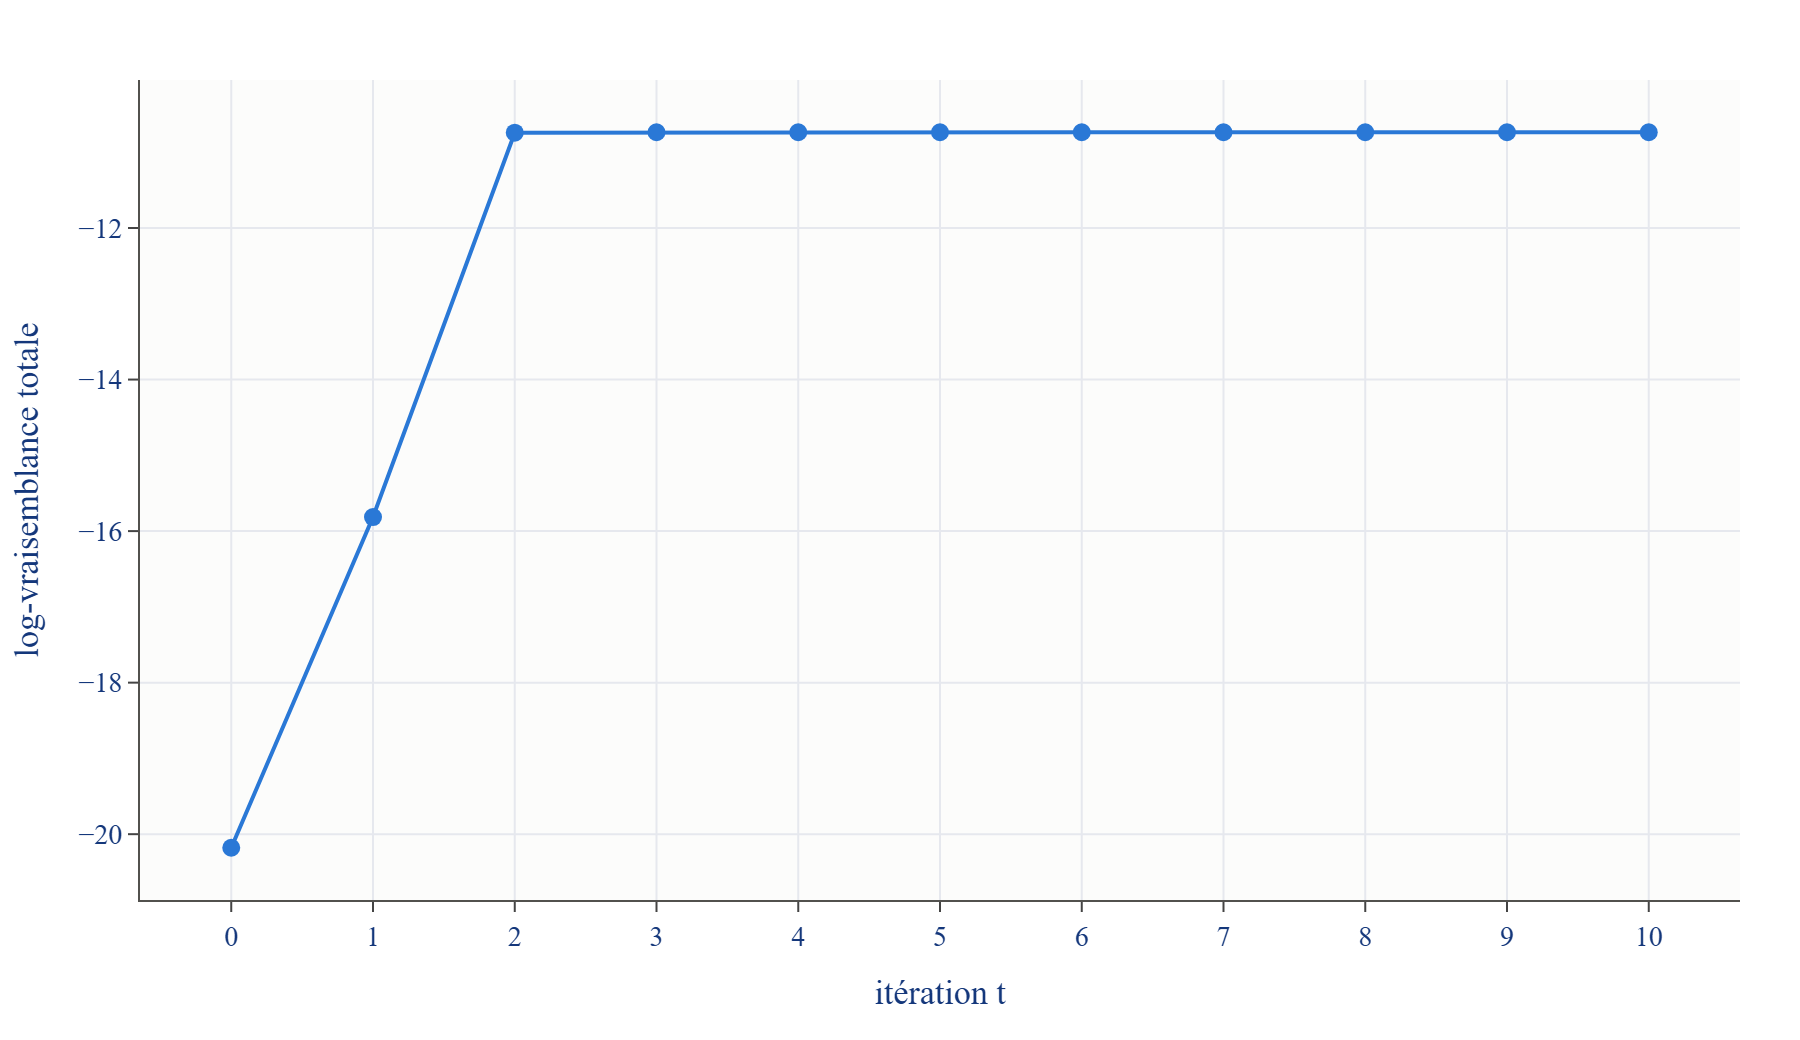
\includegraphics[width=0.85\textwidth]{figures/fig01.png}
\caption{Évolution de la log-vraisemblance au fil des itérations (exemple numérique de la section~\ref{sec:application_au_melange_gaussien_exemple}). La courbe est croissante puis stationnaire dès la troisième itération, ce qui illustre la garantie de monotonie établie à la section~\ref{sec:formulation_mathematique_complete}.f.}
\label{fig:1_1}
\end{figure}

\subsection{Exemple numérique illustratif}\label{sec:exemple_numerique_illustratif}
Afin de rendre plus concret le mécanisme d'élagage décrit à la section~\ref{sec:elagage}, reprenons l'exemple numérique de la section~\ref{sec:application_au_melange_gaussien_exemple} : les huit observations scalaires X = \{0,5 ; 1,0 ; 1,2 ; 1,8 ; 7,1 ; 7,5 ; 8,0 ; 8,3\}, qui forment visiblement deux groupes bien séparés. Appliquons cette fois l'EM variationnel avec $K_{\max} = 3$ composantes (soit une de plus que le nombre réel de groupes), un prior de Dirichlet de concentration $\alpha _{0}$ = 1/3, et des priors Normal-Wishart non informatifs ($\beta _{0}$ = 10$^{-3}$, $\nu _{0}$ = 1, $W_{0}$ = 1).

L'algorithme converge en 5 à 15 itérations selon l'initialisation (critère $|\Delta \mathrm{ELBO}| < 10^{-6}$), vers la même solution dans les dix essais réalisés (graines 0 à 4, initialisation par les hyperparamètres ou par k-means). Le tableau~\ref{tab:t1_5} présente les paramètres finaux obtenus pour chacune des trois composantes.

\tableauGenere{t1_5}
Ce résultat illustre de façon particulièrement nette le mécanisme théorique décrit à la section~\ref{sec:elagage}. Les deux premières composantes se partagent presque également la masse de probabilité (poids 0,482 chacune), avec des moyennes de 7,724 et 1,126 qui coïncident, à $10^{-3}$ près, avec les moyennes empiriques des deux groupes et avec la solution de l'EM classique de la section~\ref{sec:application_au_melange_gaussien_exemple} (7,725 et 1,125). La troisième composante, en revanche, voit son paramètre $\alpha _{k}$ rester exactement égal à sa valeur initiale $\alpha _{0}$ = 1/3 = 0,333, signe que $N_{k}$ = $\alpha _{k}$ - $\alpha _{0}$ = 0 : aucune observation, même partiellement, ne lui a été attribuée au cours de la convergence. Cette composante est donc entièrement inactive, et le modèle retient effectivement $K_{\text{effectif}}$ = 2 composantes actives, exactement le nombre réel de groupes : un résultat que l'EM classique, avec K fixé à l'avance, ne peut pas produire de lui-même : il faudrait, pour l'EM classique, comparer explicitement les solutions à K = 2 et K = 3 au moyen d'un critère externe tel que le BIC, alors que l'EM variationnel effectue cette sélection de façon endogène, en une seule exécution.

\section*{Annexe H : Tableaux détaillés des résultats}
\addcontentsline{toc}{section}{Annexe H : Tableaux détaillés des résultats}
Cette annexe rassemble trois figures du chapitre~\ref{chap:resultats} et la sensibilité des décisions d'équivalence à la marge. Les tableaux descriptifs (moyennes par bras des scénarios S1 à S7, grille de $\alpha_0$ du scénario S8, moyennes du cas pratique par plan, effectif et bras, relevés de prix écartés) et la lecture détaillée de chaque décision sont produits par le code et archivés dans le dépôt du mémoire (annexe A) : fichiers \texttt{resultats/tables/scenarios\_resume.csv}, \texttt{S8\_alpha0.csv}, \texttt{prix\_resume.csv}, \texttt{prix\_releves\_ecartes.csv} et \texttt{memoire/tables/lecture\_*.tex}.
\setcounter{table}{0}\renewcommand{\thetable}{H.\arabic{table}}\renewcommand{\theHtable}{H.\arabic{table}}

\subsection*{Figures des décisions et de la sélection du nombre de régimes}
\setcounter{figure}{0}\renewcommand{\thefigure}{H.\arabic{figure}}\renewcommand{\theHfigure}{H.\arabic{figure}}
\begin{figure}[H]
\centering
\IfFileExists{figures/fig12.png}{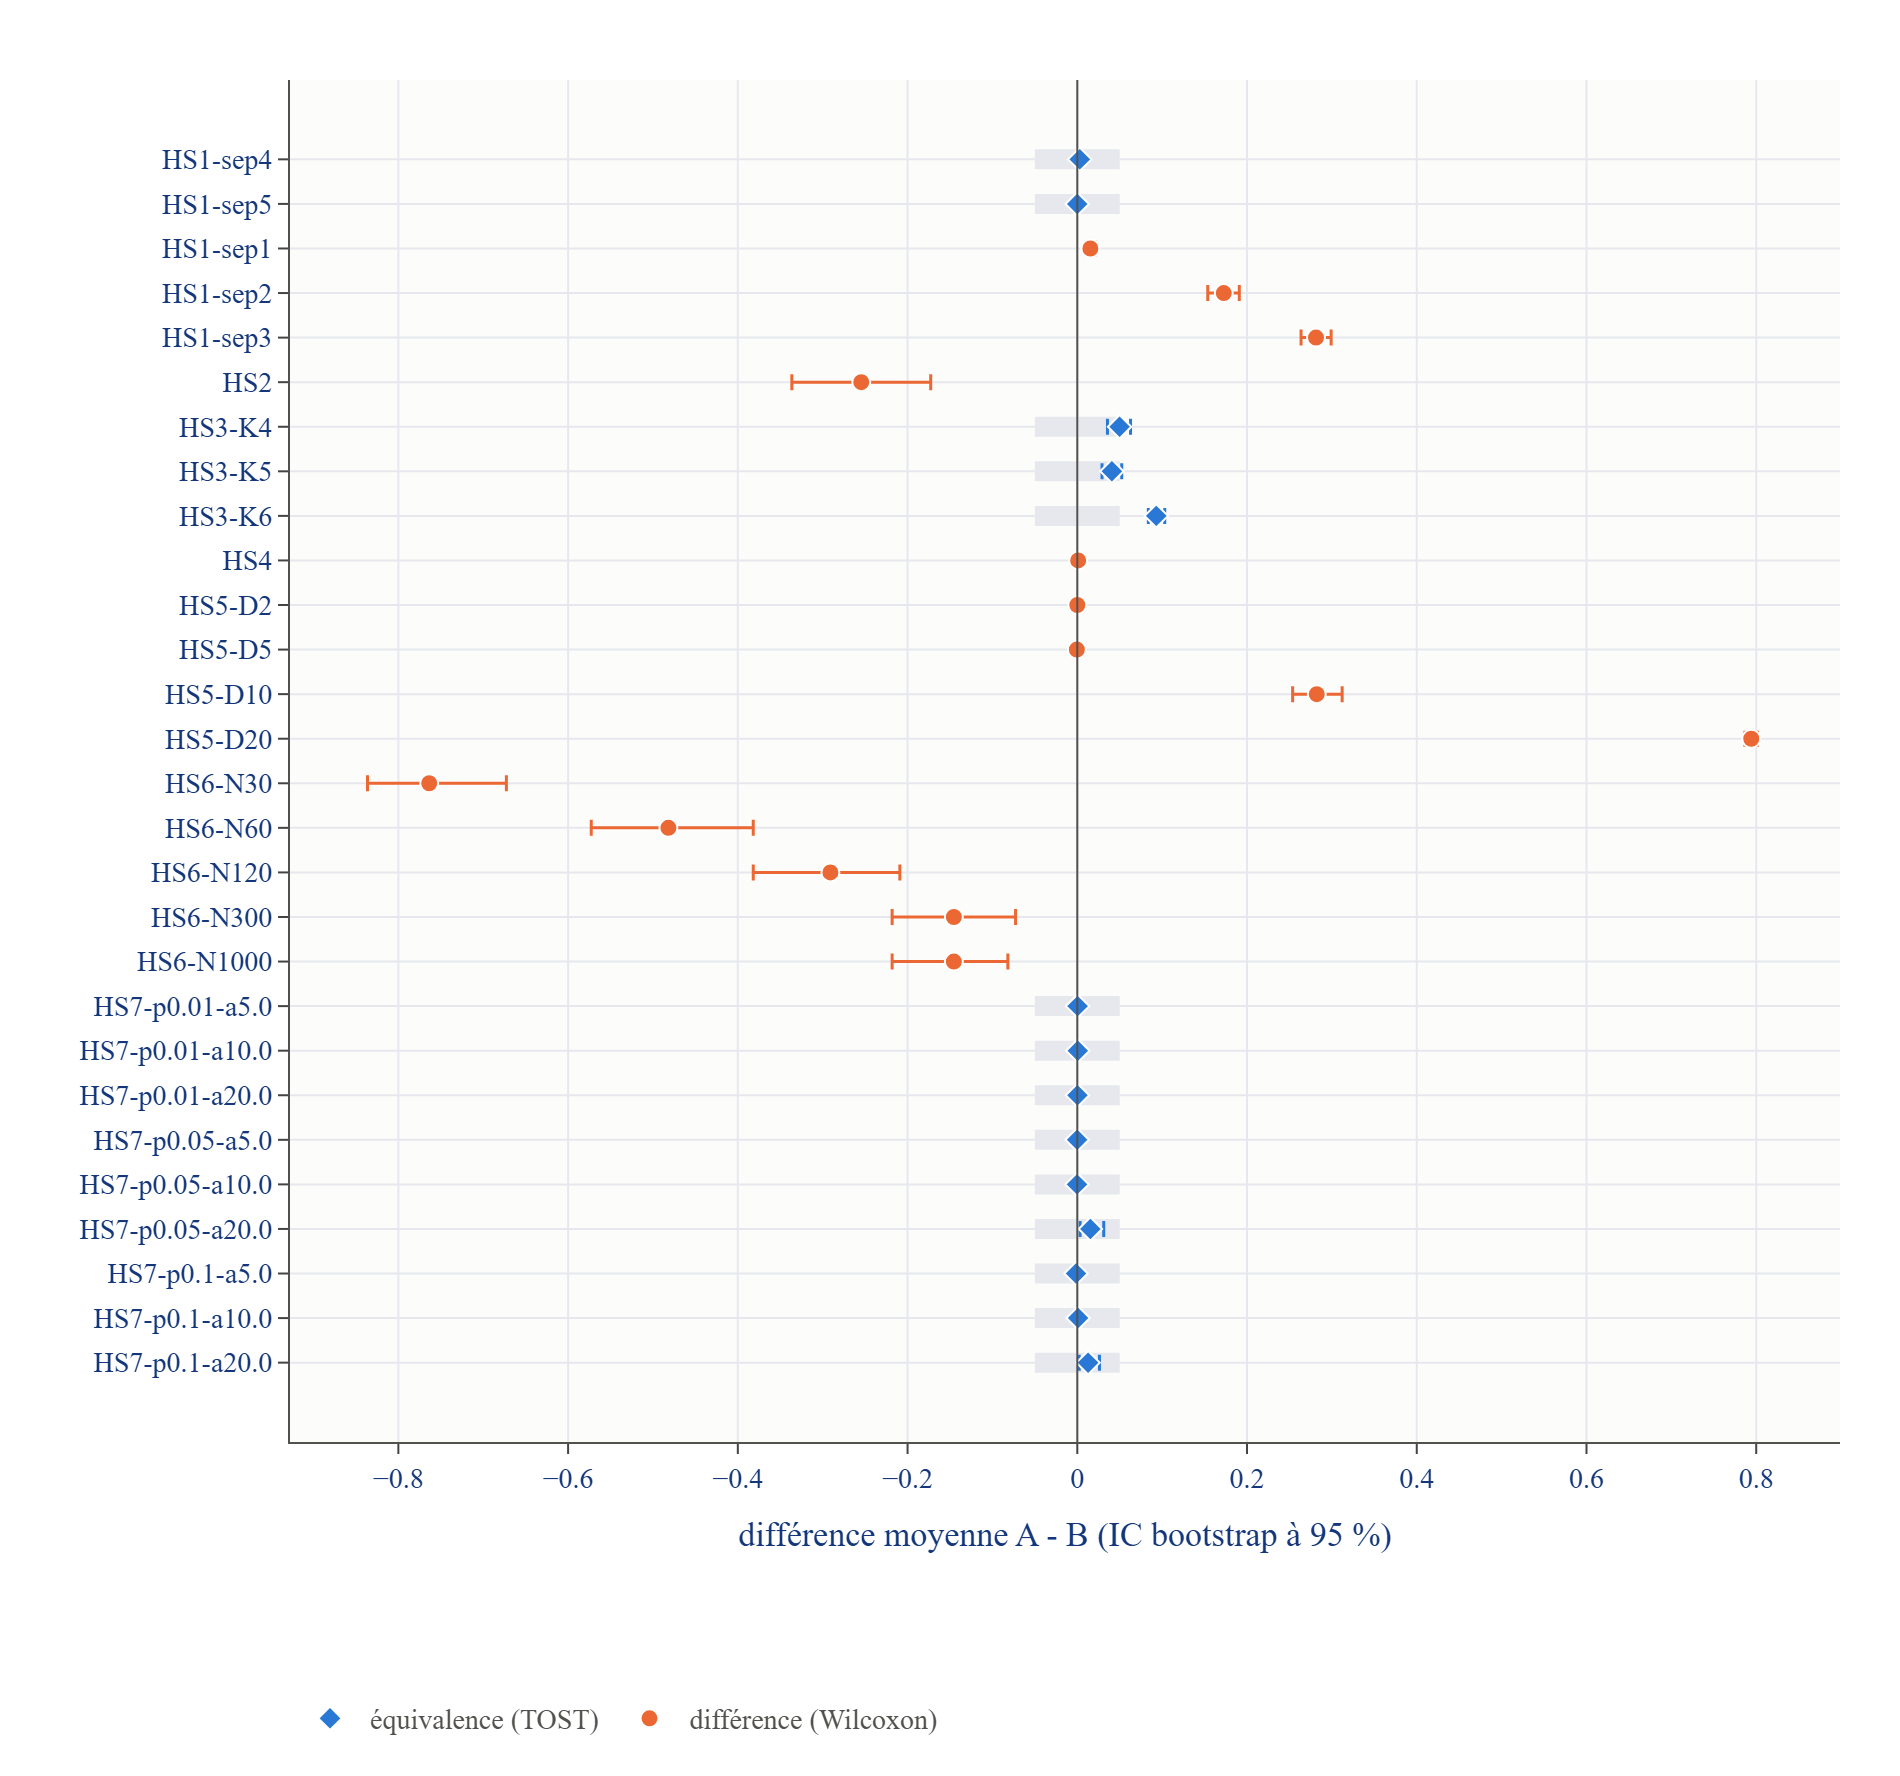
\includegraphics[width=0.9\textwidth]{figures/fig12.png}}{\fbox{\parbox{0.8\textwidth}{\centering figure à générer (\texttt{python run.py --figures})}}}
\caption{Décisions de la famille des scénarios : différence moyenne appariée (VB moins EM) et intervalle bootstrap à 95 \%, marge d'équivalence en gris.}
\label{fig:scenarios_decisions}
\end{figure}
\begin{figure}[H]
\centering
\IfFileExists{figures/prix_selection.png}{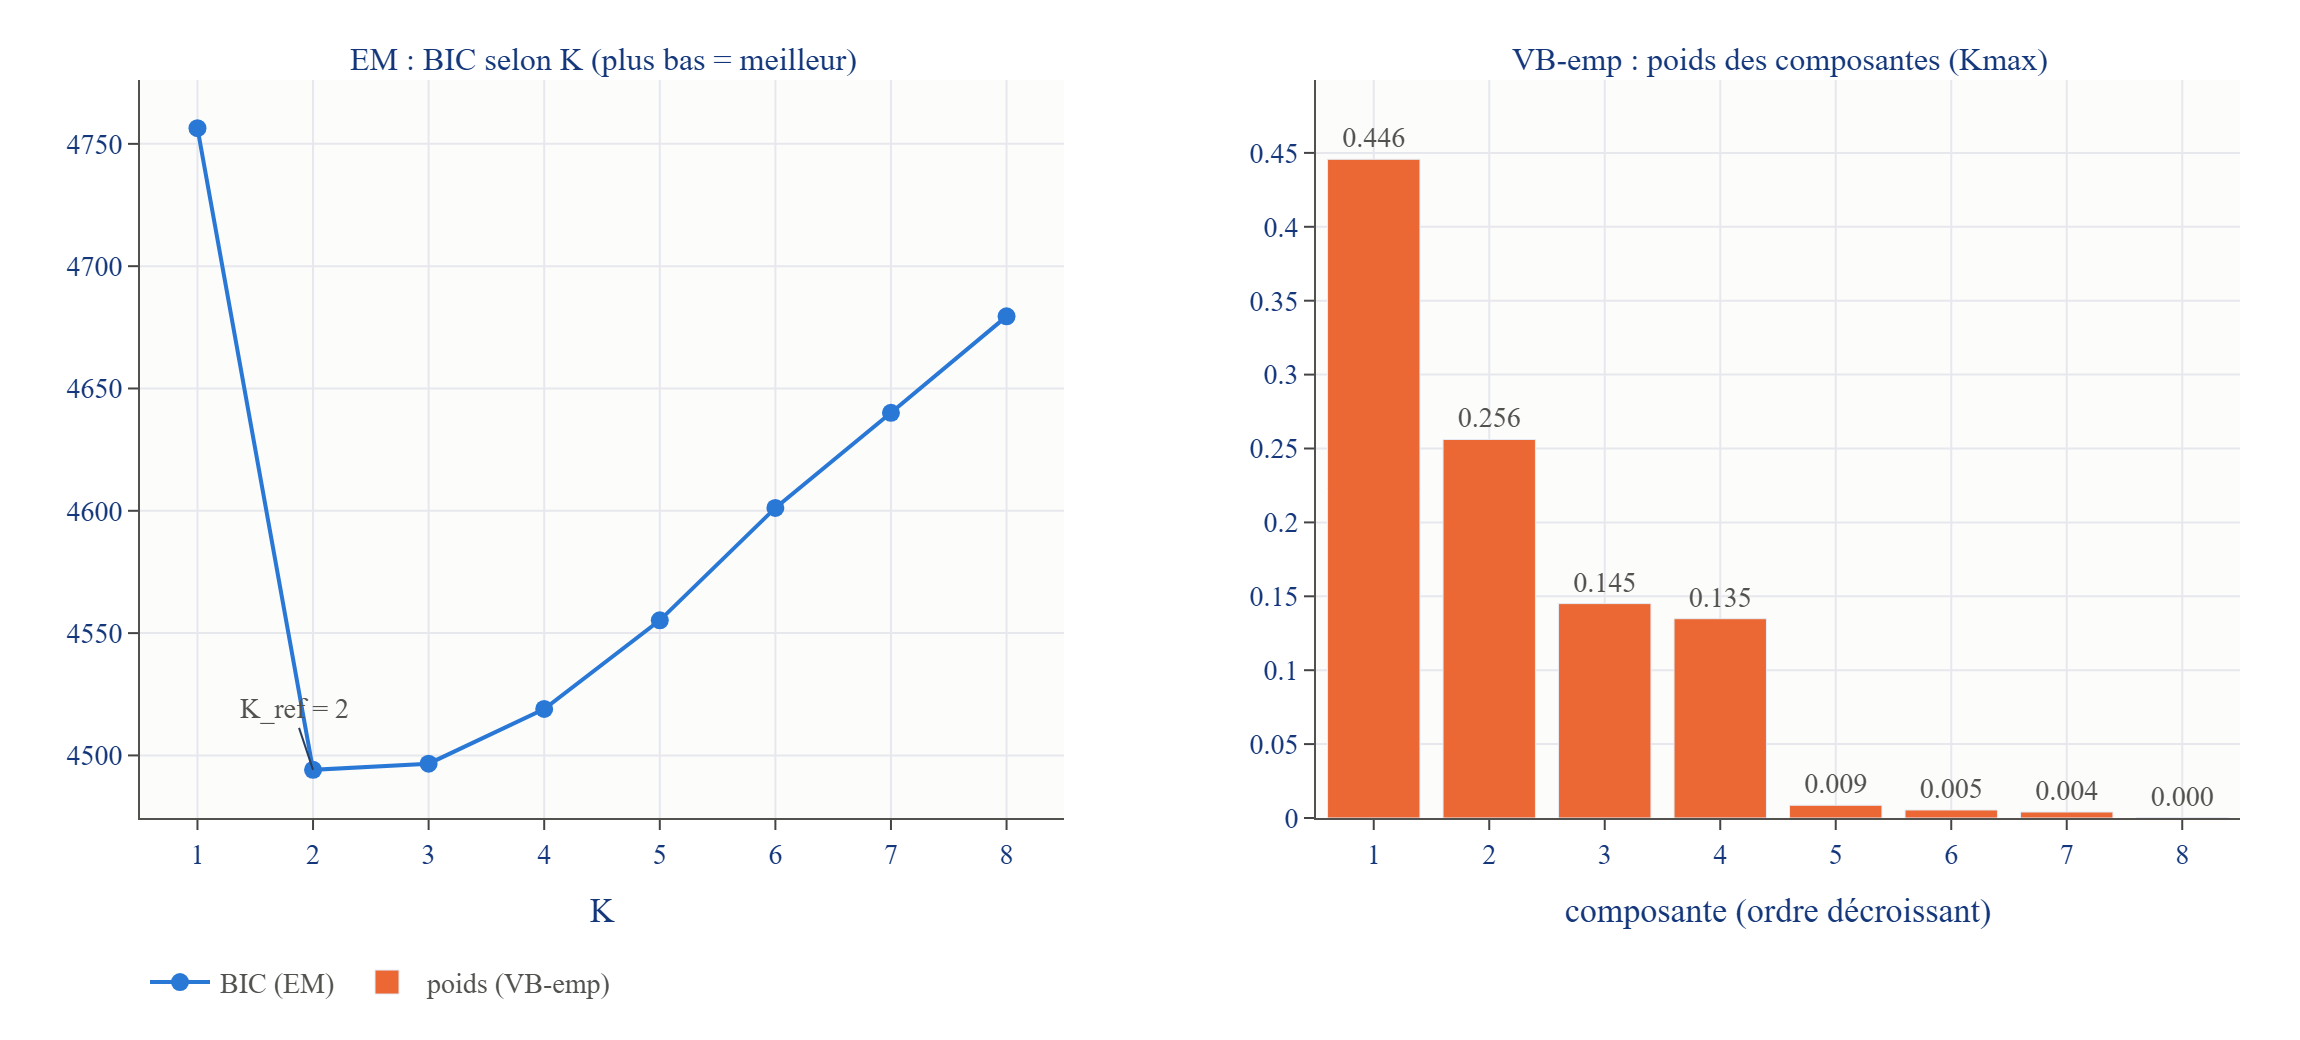
\includegraphics[width=\textwidth]{figures/prix_selection.png}}{\fbox{\parbox{0.8\textwidth}{\centering figure à générer (\texttt{python run.py --figures})}}}
\caption{Sélection du nombre de régimes sur toute la période d'apprentissage : BIC de l'EM selon $K$ (gauche) et poids des composantes du VB à priors empiriques avec $K_{\max}=8$ (droite).}
\label{fig:prix_selection}
\end{figure}
\begin{figure}[H]
\centering
\IfFileExists{figures/prix_decisions.png}{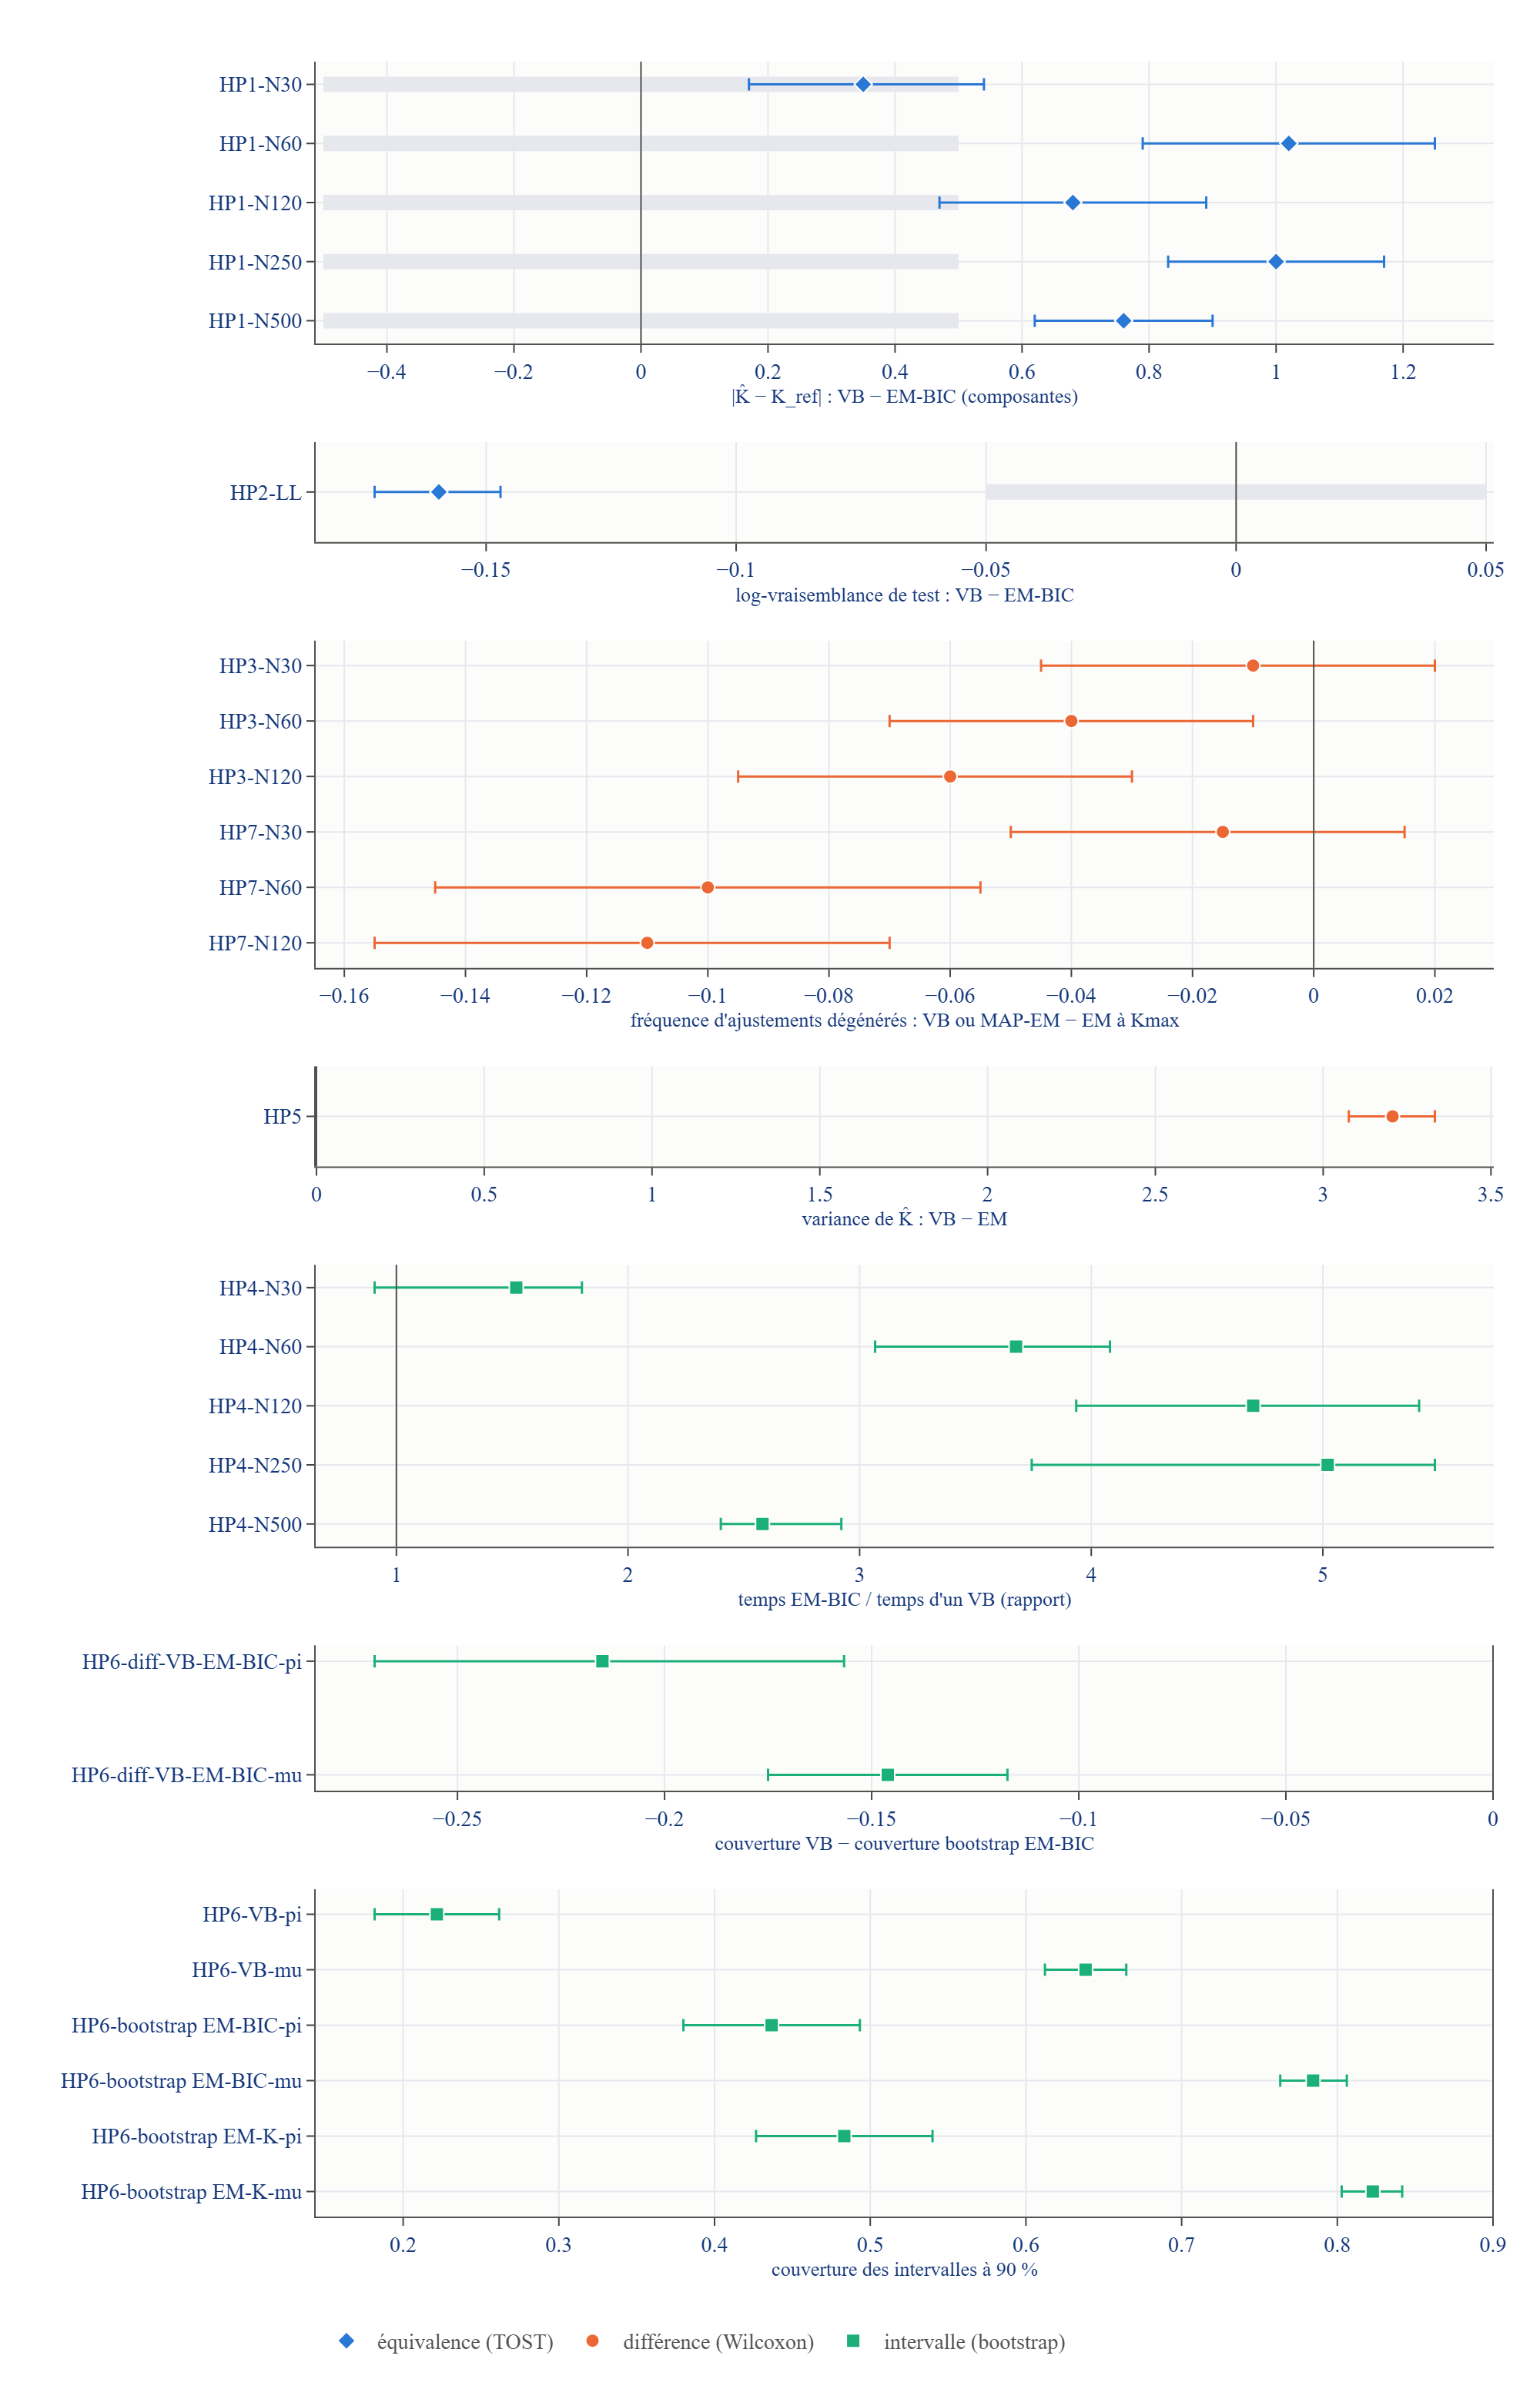
\includegraphics[width=0.9\textwidth]{figures/prix_decisions.png}}{\fbox{\parbox{0.8\textwidth}{\centering figure à générer (\texttt{python run.py --figures})}}}
\caption{Décisions de la famille « prix », un panneau par grandeur mesurée (chacun avec son unité et sa valeur de référence, trait vertical) : estimation et intervalle bootstrap à 95 \% ; bande grise : marge d'équivalence. HP4 et HP6 sont jugées sur leur intervalle (section~\ref{sec:decision}).}
\label{fig:prix_decisions}
\end{figure}

\tableauGenere{sensibilite_marges}


\end{document}
